%\RequirePackage{fix-cm}
\documentclass[smallcondensed]{svjour3}       % onecolumn (second format)
%\usepackage{titlesec}
%\titleformat{\section}{\normalfont\fontfamily{phv}\fontsize{11}{19}\bfseries}{\thesection}{1em}{}
%\titleformat{\subsection}{\normalfont\fontfamily{phv}\fontsize{10}{19}\bfseries}{\thesubsection}{1em}{}
%\titleformat{\subsection}
% {\normalfont\bfseries}{\thesubsection}{1em}{}
%\smartqed  % flush right qed marks, e.g. at end of proof
%\documentclass[manuscript,screen]{acmart}

%
% \BibTeX command to typeset BibTeX logo in the docs
%\AtBeginDocument{%
%  \providecommand\BibTeX{{%
%    \normalfont B\kern-0.5em{\scshape i\kern-0.25em b}\kern-0.8em\TeX}}}

% Rights management information. 
% This information is sent to you when you complete the rights form.
% These commands have SAMPLE values in them; it is your responsibility as an author to replace
% the commands and values with those provided to you when you complete the rights form.
%
% These commands are for a PROCEEDINGS abstract or paper.
%\copyrightyear{2018}
%\acmYear{2018}
%\setcopyright{acmlicensed}
%\acmConference[Woodstock '18]{Woodstock '18: ACM Symposium on Neural Gaze Detection}{June 03--05, 2018}{Woodstock, NY}
%\acmBooktitle{Woodstock '18: ACM Symposium on Neural Gaze Detection, June 03--05, 2018, Woodstock, NY}
%\acmPrice{15.00}
%\acmDOI{10.1145/1122445.1122456}
%\acmISBN{978-1-4503-9999-9/18/06}


%\usepackage{graphicx}
\usepackage{paralist}
\usepackage{booktabs}
\usepackage[linesnumbered,noend, noline]{styles/algorithm2e}
%\usepackage[linesnumbered,noend, noline]{algorithm2e}
\usepackage{algpseudocode}% http://ctan.org/pkg/algorithmicx
\usepackage{url}
\usepackage[gen]{eurosym}
%\setlength{\parindent}{1em}
%\setlength{\parskip}{1em}
\makeatletter
\g@addto@macro{\UrlBreaks}{\UrlOrds}
\makeatother
\usepackage{breakurl}
\newcommand{\urls}[1]{{\scriptsize\url{#1}}}

\def\it{\textit}
\def\tr{\textrm}
\newcommand{\ib}[1]{{\textbf {\textit { #1}}}}
\newcommand{\ts}[1]{{\textsc {{ #1}}}}
\newcommand{\ft}[1]{{\footnotesize {\texttt {#1}}}}
\def\tt{\ft}
\def\fs{\footnotesize}
\usepackage{wrapfig}

\def\bf{\textbf}
\def\eq {Equation~}
\def\eqs {Equations~}
\def\fig {Figure~}
\def\figs {Figures~}
\usepackage{subfig}
\newcounter{finding_counter}
\setcounter{finding_counter}{1}
\newcommand{\rcomment}[1] { \textcolor{red}{#1}}
\newcommand{\comparisoncell}[2]{
\parbox{#1\textwidth}{\vspace{3pt} #2 \vspace{2pt}}
}
\newcommand{\boxtext}[1]{
    \begin{tcolorbox}
        \textbf{Observation \arabic{finding_counter}:} #1 \stepcounter{finding_counter}
    \end{tcolorbox}
}
\newcommand{\eqrow}[1]{
    \vbox{
        \begin{equation}
            \nonumber
            \begin{split}
                #1 \hspace{10em}
            \end{split}
        \end{equation}
        } \\
     }
\newcommand{\surveyquote}[2]{\begin{adjustwidth}{1em}
{0em}\emph{\\#1}. [\##2] \\\end{adjustwidth}}
\usepackage{balance}  % to better equalize the last page
\usepackage{graphics} % for EPS, load graphicx instead
%\usepackage[T1]{fontenc}
%\usepackage{txfonts}
%\usepackage{times}    % comment if you want LaTeX's default font
%\usepackage[pdftex]{hyperref}
% \usepackage{url}      % llt: nicely formatted URLs
%\usepackage{color}
%\usepackage{textcomp}
\usepackage{booktabs}
\usepackage{ccicons}




%\usepackage{cite}
\usepackage{url}
\usepackage{fancybox}
\usepackage{multirow}
\usepackage{flushend}
\usepackage{booktabs}
\usepackage{tabularx}
\usepackage{comment}
\usepackage{array}
\usepackage[flushleft]{threeparttable}
\usepackage{mdframed}
\graphicspath{{}{images/}{dia/}}
\DeclareGraphicsExtensions{.pdf,.png}


\usepackage{listings}
%\usepackage{courier}
\usepackage{hyperref}


\newcounter{o}
\setcounter{o}{0}
\newcounter{d}
\setcounter{d}{0}
\newcounter{t}
\setcounter{t}{0}


\usepackage{tikz}
\usepackage{styles/pgf-pie}
\usetikzlibrary{positioning,shadows}
\newif\ifpienumberinlegend
\pgfkeys{/number in legend/.code=
    \expandafter\let\expandafter\ifpienumberinlegend
    \csname if#1\endcsname
    \ifpienumberinlegend
    \let\legendbeforenumber\beforenumber
    \let\legendafternumber\afternumber
    \def\beforenumber##1\afternumber{}%
    \fi,
    /number in legend/.default=true
}
%colors
\definecolor{1c1}{RGB}{188,162,6}
\definecolor{1c2}{RGB}{137,129,80}
\definecolor{1c3}{RGB}{239,167,31}
\definecolor{1c4}{RGB}{88,194,241}
\definecolor{1c5}{RGB}{6,180,188}

% stiles used
\tikzset{mynode/.style={draw=white,solid,circle,fill=green,inner sep=1pt, thick,
text=black}}
%draw=black to get a black circle, fill=white so it actually has a
%background and text=black to not get that rendered in the specified color
\tikzset{arrow line/.style={dashed, line width= 2.5pt, color=#1}}

\def\bf{\textbf}
\def\eq {Equation~}
\def\eqm {Eq~}
\def\eqs {Equations~}
\def\fig {Figure~}
\def\figs {Figures~}
\def\tbl {Table~}
\def\tbls {Tables~}
\def\ie{\textit{i.e.,}}
\def\eg{\textit{e.g.,}}
\def\sec {Section~}
\def\secs {Sections~}
\def\alg {Algorithm~}
\def\algs {Algorithms~}
\def\app {Appendix~}
\def\it{\textit}
\def\tr{\textrm}
\def\tt{\mct}
%\newcommand{\ib}[1]{{\textbf {\textit { #1}}}}
%\newcommand{\ts}[1]{{\textsc {{ #1}}}}
\newcommand{\mct}[1]{{\footnotesize {\texttt {#1}}}}

\newcommand{\qu}[1]{{\it{``#1''}}}
\newcommand{\api}[1]{{\sf{\texttt\small{#1}}}}
\newcommand{\callout}[1]{{\vspace{1mm}\noindent{\fbox{\parbox{0.97\columnwidth}{#1}}}\vspace{1mm}}}
\usepackage{paralist}
\usepackage{hyperref}
\usepackage{soul}

\normalsize
\let\labelindent\relax
\usepackage{enumitem}

\newcommand{\nd}{\vspace{1mm}\noindent}
\usepackage{caption}
%\usepackage[toc,page]{appendix}
\usepackage{tikz}
\newcommand*\circled[1]{\tikz[baseline=(char.base)]{
            \node[shape=circle,draw,inner sep=1pt] (char) {#1};}}

 \lstset{
         language=Java,
         basicstyle=\scriptsize\ttfamily, % Standardschrift
         %numbers=left,               % Ort der Zeilennummern
         numberstyle=\tiny,          % Stil der Zeilennummern
         %stepnumber=2,               % Abstand zwischen den Zeilennummern
         numbersep=5pt,              % Abstand der Nummern zum Text
         tabsize=2,                  % Groesse von Tabs
        % extendedchars=true,         %
         breaklines=true,            % Zeilen werden Umgebrochen
%         keywordstyle=\color{black},
 %   	 frame=single,
 %        keywordstyle=[1]\textbf,    % Stil der Keywords
 %        keywordstyle=[2]\textbf,    %
 %        keywordstyle=[3]\textbf,    %
 %        keywordstyle=[4]\textbf,   \sqrt{\sqrt{}} %
         stringstyle=\color{white}\ttfamily, % Farbe der String
         showspaces=false,           % Leerzeichen anzeigen ?
         showtabs=false,             % Tabs anzeigen ?
         xleftmargin=17pt,
         framexleftmargin=17pt,
         framexrightmargin=5pt,
         framexbottommargin=4pt,
         %backgroundcolor=\color{lightgray},
         showstringspaces=false,      % Leerzeichen in Strings anzeigen ?
     %    escapeinside={\%*}{*)}
 }
\usepackage{rotating}
\usepackage{pdflscape}
\lstdefinestyle{inlinecode}{basicstyle={\ttfamily\scriptsize\bfseries}}
\newcommand\code{\lstinline[style=inlinecode]}
%\newcommand{\urls}[1]{{\scriptsize\url{#1}}}
\usepackage{tcolorbox}
\newcommand{\emt}[1]{\emph{``#1''}}
\usepackage{paralist}
\usepackage[outercaption]{sidecap}    
%\usepackage{unicode-math}
\usepackage{amssymb}% http://ctan.org/pkg/amssymb
\usepackage{pifont}% http://ctan.org/pkg/pifont
\newcommand{\cmark}{\ding{51}}%
\newcommand{\xmark}{\ding{55}}%



\usepackage{enumitem}
\hypersetup{
    colorlinks=true,
    linkcolor=blue,
    filecolor=magenta,      
    urlcolor=cyan,
}
\newtcolorbox
{mybox}[2][]{colbacktitle=red!10!white,
colback=blue!10!white,coltitle=black!70!black,
title={#2},fonttitle=\bfseries,#1}

\usepackage{xcolor}
\definecolor{ao(english)}{rgb}{0.0, 0.5, 0.0}
\newcommand{\mybars}[3]{
  {\color{red}\rule{#1pt}{6pt}}
  {\color{yellow}\rule{#2pt}{6pt}}
  {\color{ao(english)}\rule{#3pt}{6pt}}
}

\usepackage{xcolor}
\usepackage{cite}
\usepackage{amsmath,amssymb,amsfonts}
% \usepackage{algorithmic}
\usepackage{textcomp}
\usepackage{float}
\usepackage{threeparttable}
\usepackage{amsmath}
\usepackage{enumitem}
\usepackage{graphicx}
\usepackage{mathtools,cuted}
\usepackage{tablefootnote}
% \usepackage{xcolor}
\usepackage{lipsum}
% \usepackage{subcaption}
\usepackage{multirow}
\usepackage{longfbox}
\usepackage{makecell}
\usepackage{longtable}
\usepackage{changepage}
% \usepackage{cleveref}
\newtoggle{comment}
\toggletrue{comment}

\newcommand{\gias}[1] { \textcolor{magenta}{\textbf{[Gias: #1]}}}
\newcommand{\partha}[1] { \textcolor{red}{\textbf{[Partha: #1]}}}
\newcommand{\anindya}[1] { \textcolor{green}{\textbf{[Anindya: #1]}}}
\newcommand{\khalid}[1]{\textcolor{blue}{\textbf{[Khalid: #1]}}}
\newcommand{\rifat}[1]{\textcolor{cyan}{\textbf{[Rifat: #1]}}}

\DeclarePairedDelimiter\abs{\lvert}{\rvert}
\newcommand{\topicquote}[1]{\\ \hspace*{2em}\emph{``#1"}}
\begin{document}
\title{A Comparative Study of Software Development Practices: \small{Understanding Similarities and Differences of Software Development Practices Between an Emerging Country and Some Developed Countries}}
\titlerunning{Software Development Practices in an Emerging Software Industry}
%\shortcite{Topics of Developers' Discussions During COVID-19 Crsis}


\author{Partha Chakroborty \and Khalid Hasan \and Rifat Shahriyar \and Anindya Iqbal \and Gias Uddin}


\institute{P. Chakroborty, K. Hasan, R. Shahriyar, and A. Iqbal \at
              Department of Computer Science and Engineering, BUET, Dhaka, Bangladesh\\
              \email{shuvopartho@gmail.com, 72.khalidhasan@gmail.com, rifat@cse.buet.ac.bd, anindya@cse.buet.ac.bd,
              }
            \and
            Gias Uddin \at
              Department of Electrical and Computer Engineering, University of Calgary, Alberta, Canada\\
              \email{gias.uddin@ucalgary.ca}
}

\date{}
\maketitle

\sloppy


\begin{abstract}
%\hfill
%\newline
\noindent\textbf{\it{Context:}}
%\anindya{Changed the context. Please check.}
Software development is complicated with rapidly changing requirements, techniques, processes and 
the involvement of diverse stakeholders (clients, developers, testers, managements, and so on). 
It is often the case a burgeoning community shapes around the emergence of a software industry 
in a location (e.g., silicon valley) or in a country. Therefore, 
a study on the software development practice in the industry of a country
reveals the challenges and scopes of improvement for that industry and
industries of similar types. There are several studies on the software industry
of developed countries. However,
to the best of our knowledge, no recent study explores the issues
of an emerging software industry. 
% The software engineering industry in Bangladesh offers a rapidly emerging
% environment and significantly contributes to the national economy. A thorough
% study to understand the software development practices is essential to figure
% out the challenges and opportunities to deliver high-quality software.
\textbf{\it{Objective:}} We focus on understanding the challenges and opportunities within the software companies of Bangladesh, which is an emerging developing country with a large group of skilled software practitioners. We have two objectives. First, we aim to understand the methods and practices used
in the dynamic environment of software development. This analysis informs us of the practices adopted and challenges faced by the software companies in an emerging country. Second, we aim  to understand whether and how the development practices 
and methods in Bangladesh differ from other countries. The comparison informs us of the 
uniqueness of software industries in emerging countries like Bangladesh. 
\textbf{\it{Method:}} Our study has four phases. First, we conduct a series of
semi-structured interviews with eight individual practitioners from four
software companies. The purpose is to understand the overall development
practices and methods. Second, we use the insights gained from the first phase
to design a survey. A total of 137 software practitioners from a diverse set of
companies responded to the survey. Third, we analyze the survey responses to learn about the development 
practices in Bangladesh. Fourth, we compare our findings against findings previously reported for other countries (e.g., European countries, Canada, 
Neew Zealand, etc.).
\textbf{\it{Results:}} The major findings of our study on the companies of
Bangladesh software industry are: i) Most companies follow agile methodology
and give implementation-related activities a high priority, ii) Most companies
are used to developing web-based software products, iii) Most companies use less
automated testing and deployment tools, and iv) Several companies seriously
consider the security, performance, and scalability of their software. 
The development practices in Bangladesh are mostly similar to other developing countries (e.g., Malaysia), but differ from 
those in developed countries (e.g., Japan, Canada, Europe, etc.). For example, due to the mostly outsourcing nature of work carried in Bangladesh, 
overall system design is not as highly practised. 
Automated testing is also is not as widely practiced in Bangladesh as the developed countries, partly due to the difficulty of 
testing web-based systems which are mostly developed in Bangladesh. The companies in Bangladesh also lags
behind in the area of automated performance testing and containerization that
might ensure resource-optimized scalability. \textbf{\it{Conclusions:}} The findings 
can guide software practitioners to improve development practices in emerging countries and software 
providers with new new tool support to assist in the process. In particular, more emphasis can 
be placed upon promoting overall system design and automated testing in the software industries of emerging countries.  
\end{abstract}
\keywords{Survey, Software Development Practices and Challenges, Emerging Countries}


\section{Introduction}
\label{introduction}

%The software engineering (SE) industry in Bangladesh is considered relatively small compared to the size of its population (160 million-plus) and the size of the national economy. %Yet, the software industry in this country has started rapidly emerging and become part of Bangladesh's rapid development in recent years. 
%The majority of software companies were established after 2000 and have become a crucial resource for the economy of Bangladesh \cite{Basis2017}, and also the growth rate is expected to continue sharply. This propitious growth is bolstered by export trends and a large demand for IT automation in the domestic market. To continue this achievement by fulfilling the growing expectations of software consumers, the SE industry needs to follow standard practices in producing good quality software products. %Thus for this, we have to first point out how the software development process is exercised in such a rapidly emerging industry. 

%The practice of software development varies from region to region. A certain methodology may become more efficient in some regions but is not considered efficient in other regions. Although most of the factors behind software development are the same all the time, there are certain points that vary from region to region. For software development professionals, deciding on processes, practices, and techniques is critical. Sometimes, these decisions might be based on marketing and literature bias that supports the new or industry-supported practice.

%Many studies concerning the practices of software development have been conducted. Those studies convey similarities, but also differences in diverse regions, countries, and communities. Previous empirical studies have gone into how software development practices were conducted in North America, Europe, Turkey, New Zealand, etc. There are some prior studies on the Bangladesh software engineering (SE) industry, but the studies' focus and dimension were different. To the best of our knowledge, this is the first study to identify software engineering practices in emerging countries by taking the software industry in Bangladesh as a case study on how the software industry in an emerging environment works, the challenges they face, and the practices they adopt.
% The delivery of quality outcomes on time with a competitive budget is a major
%  challenge for the software industry. The practice of state-of-the-art SE
%  methods and technologies is indispensable to achieve success. 
 A study on the software development practice in a country
can reveal the challenges and scopes of improvement for software industries of similar countries. There are several studies on the software
industry of countries that focused on understanding the software development practices 
in developed countries and/or countries with matured software industry (e.g., Japan, Canada)~\cite{Garousi2013, Garousi2015, Vonken2012, Wang2018}. However, 
the software industry of a developed country differs from that of a developing
country in many aspects. Easy migration opportunities of the developers cause
constant scarcity of experienced people in developing countries. Still, due to
the abundance of Computer Science graduates, the software industry of some
developing countries are continuing to emerge by catering to the majority of the
local market as well as expanding in the global market.


A recent study 
focused on the software development ecosystems in Malaysia~\cite{Baharom2006}. However, the study 
did not consider the diverse development practices (e.g, security, scalability in development practices). There 
is also no study on a systematic comparison of the software development practices in the software industries 
between the developing and developed countries. In this paper, we focus on understanding the software development 
practices in an emerging software industry 
by analyzing those practices in another developing country, Bangladesh. Like Malaysia, 
Bangladesh is also a rapidly growing economy with 160 million
population. IT sector is considered a priority sector in Bangladesh over the
last decade. The software development industry dominates this sector. According to the
Bangladesh Association of Software and Information Services (BASIS), 1100+
software companies operate in Bangladesh, where around 40\% have a global
business. The foreign revenue earned by the industry is over 800 Million
USD~\cite{BASIS2018}. Therefore, an understanding of the development practices in Bangladesh and a comparison of such practices 
with other countries can inform us of the issues and characteristic of an emerging software industry.
% In particular, our aim is to figure out the similarities and dissimilarities
% in the development practices of Bangladesh with other countries, which would
% eventually reveal the areas where this industry needs improvement in such emerging countries.
 
% The purpose of this research is to systematically study and characterize the Software
%  Engineering (SE) practices in Bangladesh, i.e., the tools and technology used
%  for design, development, testing, and deployment. Similar studies were carried
%  out in other countries such as Canada, Turkey, Netherlands, and New Zealand. The
%  current study thus also situates a comparative picture of SE practices in Bangladesh
%  and other countries. In particular, our aim is to figure out the similarities and dissimilarities
% in the development practices of Bangladesh with other countries, which would
% eventually reveal the areas where this industry needs improvement in such emerging countries.
 
Our study has four steps. First, we conduct a series of semi-structured interviews of eight software professionals from four 
leading software companies in Bangladesh. We corroborate the interview findings with findings from similar studies of 
other countries like 
Canada, Turkey, Netherlands, New Zealand, etc.~\cite{Garousi2013, Garousi2015, Vonken2012, Wang2018}. 
The purpose is to gain an overview of the overall development practices and challenges. 
Second, we design a survey based on the insights gained from the interviews. A total of 137 
software practitioners from diverse software companies in Bangladesh responded to the survey. Third, 
we analyzed the survey responses to understand the software development practices and challenges in Bangladesh. Fourth, 
we compare our findings against findings from other countries. We answer two research questions:
\begin{inparaenum}[(RQ1)]
  \item What are the software development practices in an emerging country like Bangladesh?
  \item How do the development practices in Bangladesh differ from other countries?
\end{inparaenum} We report the practices (RQ1) and the comparisons (RQ2) along four dimensions (D) as follows. The four dimensions 
were previously used in similar country-based previous studies, which thus helped us to compare our findings against their findings.

\begin{description}
\item[\bf{D1. Software development methodologies used.}] We investigate the development
approaches, methodologies, and requirements analysis processes. We find that the software
companies in Bangladesh mostly follow the agile methodology. In comparison with the
other countries, Bangladeshi software companies generally spend
more time on the implementation stage of the development. Technologically advanced countries spend more on system design.
\item[\bf{D2. Software tools and techniques used}.] We determine the
trending technologies like technology platforms, programming languages,
frameworks, etc. We find that web-based software services
are prevalent in the Bangladeshi software market and JavaScript is mostly used language for web
development. The degree of technologies and tools usage varies
from the developed countries due to the availability of experienced developers,
budget, etc. 
\item[\bf{D3. Software testing and devops practices used}.] We explore the
present situation of testing and deployment practices adopted by the software
firms in Bangladesh by asking questions about testing and deployment tools, test
automation level, version control system, etc. We find
that the usage of test automation and deployment tools is not widespread in the
Bangladeshi industry. We also see that compared
to developed countries, the test automation tool adoption is inadequate. 
\item[\bf{D4. Security and performance measures used}.] We analyze how
software companies secure and maintain their code and what practices are
followed to ensure performance and scalability. The responses show that
standards are followed for security assurance, tools are used for performance
testing, and scalability is mostly ensured by using cloud services. However, the companies in Bangladesh lags
behind in the area of automated performance testing and containerization that
might ensure resource-optimized scalability.
\end{description}

% \begin{itemize}[leftmargin=10pt]
% 
%     \item \textbf{Software methodologies used in your project?}
%     
%     We investigate the development approaches and methodologies, requirements analysis processes, etc. It helps us to analyze the dominant practice of the industry and found that the software companies mostly follow the agile development model. In comparison with the other countries, it is found that Bangladeshi software companies generally spend significant time on the implementation stage of the development whereas technologically advanced countries spend more on system design and planning.
%         
%     \item \textbf{Which implementation technologies and tools are adopted by software development professionals?}
%         
%     This is to find out the current trending technologies like technology platforms, programming languages, frameworks, etc., in the software industries of Bangladesh that may help one who wants to pursue his career here. We have found that web-based software services are prevalent in the market and JavaScript is mostly used language for web development. The degree of use of different technologies and tools usually vary from country to country due to the availability of experienced developers, budget, etc. Hence, we are interested to explore if the companies in Bangladesh deviate from world standards for particular application domains.
% 
% %\anindya{One line result summery is there for last 2 RQs. For consistency, something should be mentioned for the first two as well.}\khalid{added}        
%         
%     \item \textbf{What type of testing and deployment practices are used?}
%         
%     We want to explore the present situation of testing and deployment practices adopted by the software firms in Bangladesh by investigating testing and deployment tools, test automation level, version control system, etc. This investigation enables us to find out if there is a need for improvement in these areas. We have observed that using test automation and deployment tools is not widespread in the industry, but there is scope of improvement in others. We also see that compared to developed countries, the test automation tool adoption is inadequate. This finding is expected to motivate practitioners to use automated tools for testing.
%         
%     \item \textbf{How are the security and performance ensured in a product of a company?}
%         
%     We try to understand how software companies secure and maintain their code and what practices are followed to ensure performance and scalability. The responses show that standards are followed for security assurance, tools are used for performance testing, and scalability is mostly ensured by using cloud services. In the comparative analysis with the reputed industry, the companies in Bangladesh lags behind in the area of automated performance testing and containerization that might ensure resource-optimized scalability.     
%    
%     %\item \textbf{What software methodology are used in your project?}
%     
%   %  \anindya{The above two comments do not make much sense to me. Please rephrase.}\khalid{updated}
%     
%  %   \item \textbf{Which implementation technologies and tools are adopted by software development professionals?}
%      %   \item \textbf{What types of testing and deployment practices are used?}
%     
%     %\item \textbf{How are the security and performance ensured in the products of a company?}
%     
% \end{itemize}



%\anindya{Gias bhai suggests that we should say that we have 2 research questions. We explore these two from 4 dimensions. In this way we can make the following discussion more precise.}

%More specifically, we answer the following research questions around the two studies:
%We studied from two perspectives: (1) Understanding development practices in Bangladesh: We aim to perceive what methodologies, technologies, and testing practices are followed in software companies. (2) Comparison among the countries: We aim to figure out both similarities and dissimilarities in the development practices of Bangladesh with other countries, which would eventually reveal the areas where this industry needs improvement.
% We want to explore two research questions in this study:
% 
% \begin{itemize}[leftmargin=10pt]
%  
%  \item \textbf{What are the major characteristics of software development practices and methods in Bangladesh?}
%     
%  \item \textbf{What are the similarities and differences in software development practices between Bangladesh and other countries?}
% 
% \end{itemize}

%We explore these research questions from the following 4 dimensions.


% Our findings show that the software companies in Bangladesh usually spend most
% of the time on the implementation stage rather than system design and
% requirement analysis. Also, the use of automated testing and tools for automatic
% deployment is quite low though nowadays, it is an integral part of a better and
% standard software development practice across the globe. Besides, we compare the
% development processes of Bangladesh with other countries and analyze them from
% several perspectives. 
The findings can help software practitioners to
improve development practices in Bangladesh, which then can be applied to other developing countries with similar 
characteristics. The comparison with the developed countries shows the particular avenues for improvement in the emerging countries. 
We also notice the popularity of using cloud services across the software industries in Bangladesh. 
While this is not surprising, it nevertheless can motivate cloud providers to invest in usable and 
readily available automated software design and testing tools into the cloud to cater to the needs of 
emerging software industries. Finally, our study catalogs the
technologies and tools currently being used in Bangladesh's software firms, which could be 
useful for current students to prepare themselves for a career in this emerging software industry.

% For a software development company, the choice of technology evolves over time
% and varies widely according to application type. This study is likely to benefit
% different stakeholders such as potential local and global clients, students,
% i.e., future practitioners, etc. by presenting relevant industry practice.
% Another major benefit of such a study is having insight into different
% dimensions of industrial practice that help design better curriculum for current
% students and reveal the need for continuous education components for existing
% practitioners.
% 
% This study aims to consider detailed activities beyond high-level practices
% gathered through surveying individual professionals. The survey was conducted in
% two phases, a limited primary survey with selected respondents and a final
% survey. The goal of the primary survey was to find any discrepancy or ambiguity
% in the survey questions. Also, the primary survey had an interview session with
% each respondent. From the findings of the interviews, the question of the survey
% was later adjusted. The survey is designed to reveal the methodology of software
% development practices, the adoption of technologies and tools by the
% professionals, and the use of testing and deployment practices in the company
% where the individual concerned works.


\noindent\textbf{Paper Organization.} The remainder of the paper is organized as
follows. Section~\ref{related_works} presents the related work to our study.
Section~\ref{study_setup} describes the background of our study and the data
collection procedure. Section~\ref{study_results} answers the two research questions. Section~\ref{discussions} reports
challenges and opportunities as well as analysis by several dimensions of
the findings. Section~\ref{implications} discusses the
implications of our findings. Section~\ref{validity} discusses the threats to
validity. Section~\ref{conclusion} concludes the paper.

\section{Related Works}
\label{related_works}
% \section{Related Work}
% \subsection{Studies of Development Practices and Processes}
% any survey that did not focus on specific region but tried to look at the theme in general.
% \subsection{Related Region-specific Studies}
% NZ, Turkey, Canada, etc. any previous study in Bangladesh?
This section presents the related works that focus on software development practices and processes globally and in specific countries and regions.  

\subsection{Studies of Development Practices and Processes}
\label{dev practice study}
Cusumano et al.~\citep{Cusumano2003} have conducted a global survey on a completed software engineering project to identify software engineering practices. They have found that detailed architectural design and documentation is a common practice worldwide except the USA. In the USA, only 32\% of projects used detailed design specifications. One of the interesting findings of their study is the completeness of design before coding negatively correlates with the number of defects.

AlSubaihin et al.~\citep{AlSubaihin2019} have identified the influence of the app store on software engineering practices. They have found that the perception of quality is slightly different among app store developers. App Store developers gave more priority to user rating than the traditional metrics like code quality and documentation when measuring software quality.

To identify the state of the practices in start-up companies, Klotins et al.~\citep{Klotins2018} have conducted a study on start-up companies. They found that start-ups apply market-driven requirements engineering instead of the standard software engineering requirement engineering. However, the applied requirements engineering practices are often rudimentary and lack alignment with other knowledge areas (such as design).

\subsection{Related Region-specific Studies}
\label{region specific study}

In 2012, Vonken et al.~\citep{Vonken2012} surveyed Dutch software producing organizations to determine whether there is a gap between the current state of the practice and state of the art in software engineering. From 99 respondents, they extracted 22 interesting observations. These observations mark insights into the development process that they found unusual or surprising, at least from an academic perspective. This unusualness could either stem from certain principles being applied less or more frequently than expected or from unexpected correlations observed between factors.

The survey conducted by Garousi et al.~\citep{Garousi2015} studies Turkey's software practices to characterize and understand the state of its SE practices. The military and defense software sectors are quite prominent in Turkey, especially in the capital Ankara region, and many SE practitioners work for those companies. 54\% of the participants reported not using any software size measurement methods, while 33\% mentioned that they had measured lines of code (LOC). In terms of effort, after the development phase (on average, 31\% of overall project effort), software testing, requirements, design, and maintenance phases come next and have similar average values (14\%, 12\%,12\%, and 11\% respectively). Respondents experience the most challenge in the requirements phase. As a rather old but still widely used life-cycle model, the Waterfall is the model that more than half of the respondents (53\%) use. The next most preferred life-cycle models are incremental and Agile development models with 38\% and 34\% usage rates, respectively. The Waterfall and Agile methodologies have slight negative correlations, denoting that if one is used in a company, the other will less likely to be used.
A recent survey conducted by Wang et al.~\citep{Wang2018} in 2018 shows that New Zealand professionals use similar methodologies as professionals in other countries. Key findings of their study are, (1) popular programming language in the New Zealand software industry does not match with the worldwide ranking of popular languages, and (2) most of the time in SDLC is spent on implementation-related activities rather than analysis and design.

In another study, Groves et al.~\citep{Groves2000} reported that the New Zealand software industry pays particular attention to requirements gathering. They surveyed a selection of software companies with a general questionnaire and then conducted in-depth interviews with four companies. They found a clear difference in the testing phase between large and small software companies. Their finding is larger companies pay more attention to testing than smaller companies.

The study conducted by Sison et al.~\citep{Sison2006} presents exploratory survey and case study results on software practices of some software firms in five ASEAN countries (Malaysia, Philippines, Singapore, Thailand, and Vietnam). They found that most of the firms in that region do not follow the standard procedure for SQA.
In a study focusing on the test practices in Canadian firms, Garousi et al.~\citep{Garousi2013} found that the number of passing user acceptance tests and the number of defects found per day are considered the most important quality assurance metrics in Canadian firms. They compared their result to a previous study and showed that Canadian firms are giving more importance to testing related training than in the past.

Baharom et al.~\citep{Baharom2006} had conducted a study on Malaysian software firms to find the effectiveness of standard practices. They found that alpha and beta testing was hardly implemented in software firms. Another interesting finding of their study is that most Malaysian firms emphasize implementation; only a negligible number of companies spend more than 20\% of the effort in planning and design.
Zafar et al.~\citep{Zafar2018} have surveyed why Pakistani software firms do not follow the standard requirement engineering process. They have found multiple factors contributing to the issue, such as lack of budget, lack of time, lack of dedicated team, etc. However, the most prevalent issue is lack of budget; more than 60\% of their respondents have responded that the standard requirement engineering process was not followed due to scarcity of budget.

Based on a 200 participants survey, Hussain et al.~\citep{Hussain2020} concluded that computer science undergraduate education system in Bangladesh leaves most of its graduates unprepared for the software industry. They suggested that updating the syllabus as part of the curriculum and including internships could help make graduates fit for the industry.

To identify the software engineering practices in Bangladesh, Rahim et al.~\citep{Rahim2017} have surveyed 41 practitioners in the Bangladesh software industry. One of their interesting findings is the waterfall model is still popular among them. They found that 40\% of respondents indicated that requirement analysis and prioritization are the most challenging software development process. In another survey focusing on testing practices in the Bangladesh software industry, Bhuiyan et al.~\citep{M2018} found that most companies do not follow any standard SQA techniques for their projects. The interesting fact is such malpractice does not hinder their progress; they reported that these firms are in the industry for 6.5 years on average. However, in another survey, Begum et al.~\citep{Begum2009}  found that 47.5\% of respondents follow standard SQA techniques in their projects.
\section{Study Setup}
\label{study_setup}
% \section{Study Setup}
% overview
% \subsection{Participants}
% how the participants are selected, what is the response rate? 
% any incentives were provided to encourage participation?
% \subsection{Data Collection and Analysis}
% how was the data collected (Google form), how was the data analyzed (open coding for open-ended questions, statistical analysis for closed questions) see \url{https://ieeexplore.ieee.org/abstract/document/8658125}

Our study has four steps as follows:
\begin{itemize}[leftmargin=10pt]
  \item\bf{Step 1 - Interview (Section \ref{sec:interview}).}  We conduct a series of semi-structured interviews to understand the current development practices in Bangladesh and to understand how 
  such practices could differ from other countries. 
  \item\bf{Step 2 - Survey (Section \ref{survey_participants}).} We design a survey questions to get deep insights on the insights collected from the interviews.  
  \item\bf{Steps 3, 4 - Data Analysis to answer RQ1 and RQ2 (Section \ref{survey_data_collection}).} We analyze the
  survey responses to answer RQ1 (understand development practices in
  Bangladesh) and RQ2 (compare the practices against other
  countries).
  
\end{itemize} %We discuss the steps below.
\subsection{Interview}\label{sec:interview}
The goal of
the interview session was to prepare the survey questions. Eight individual participants from four leading software companies were
interviewed. First we designed an initial list of survey questions in Google form by consulting previous studies in other countries like 
Canada, Turkey, Netherlands, New Zealand, etc.~\citep{Garousi2013, Garousi2015, Vonken2012, Wang2018}. Each
participant was asked
to identify ambiguities in the question. From the feedback of the
interview session, we revised the questions. Each interview session lasted about half an hour. 
Interviewees were first asked to complete the survey.
After completing the survey, we asked what he/she understood from the questions
and what he/she meant by the answers. Throughout the interviews, we identified
discrepancies between the understanding of the interviewee and the goals of the
survey questions by comparing the interview findings against findings from related work.
%Finally, we adjusted the survey questions to reduce ambiguity in survey questions.
\subsection{Survey Participants}
\label{survey_participants}

\newcolumntype{v}{>{\hsize=.08\hsize}X}
\newcolumntype{b}{>{\hsize=.77\hsize}X}
\newcolumntype{m}{>{\hsize=.15\hsize}X}
% \newcolumntype{y}{>{\hsize=.33\hsize}X}
\begin{table}[htbp]
    \centering
    \caption{The survey questions (without demographic questions) along the first two dimensions (D). Subscript with a question number shows number of responses.}
    \begin{tabularx}{\textwidth}{v|m|b}
        \hline
        \bf{RQ1 D1} & \bf{Question type} & \bf{Software development methodologies used} \\ 
        \midrule
        
        \multicolumn{1}{v|}{$6_{127}$} & \multicolumn{1}{m|}{Closed} & Which of the following software development methodologies do you follow? \\ 
        \cmidrule{2-3} 
        
        \multicolumn{1}{v|}{$7_{120}$} & \multicolumn{1}{m|}{Closed} & Which of the followings do you use for requirements gathering? \\ 
        \cmidrule{2-3} 
        
        \multicolumn{1}{v|}{$8_{126}$} & \multicolumn{1}{m|}{Closed} & On which software development activities, do you spend most of the time?\\ 
        \cmidrule{2-3} 
        
        \multicolumn{1}{v|}{\bf{RQ1 D2}} & \multicolumn{1}{m|}{\bf{Question type}} & \bf{Software tools and techniques used} \\
        \midrule
        
        \multicolumn{1}{v|}{$9_{128}$} & \multicolumn{1}{m|}{Closed} & Which of the following technologies do you have experience working in?\\ 
        \cmidrule{2-3}
        
        \multicolumn{1}{v|}{$10_{127}$} & \multicolumn{1}{m|}{Closed} & What is the primary operating system you are developing on?  \\
        \cmidrule{2-3} 
        
        \multicolumn{1}{v|}{$11_{128}$} & \multicolumn{1}{m|}{Closed} & Which programming languages are you using?\\ 
        \cmidrule{2-3} 
        
        \multicolumn{1}{v|}{$12_{109}$} & \multicolumn{1}{m|}{Closed} & Which frameworks are you using?\\
        \cmidrule{2-3} 
        
        \multicolumn{1}{v|}{$13_{125}$} & \multicolumn{1}{m|}{Closed} & Which IDE are you using?\\  \hline
        
    \end{tabularx}
    \label{table:survey_questions_1}
\end{table}
The survey questions are shown in Table \ref{table:survey_questions_1}. There are 17 questions, 14 closed and three open-ended.
We targeted developers who are currently working in the
software industry of Bangladesh. 
%
\newcolumntype{v}{>{\hsize=.08\hsize}X}
\newcolumntype{b}{>{\hsize=.8\hsize}X}
\newcolumntype{m}{>{\hsize=.12\hsize}X}
% \newcolumntype{y}{>{\hsize=.33\hsize}X}
\begin{table}[tbp]
    \centering
    \caption{The survey questions (without demographic questions) along the last two dimensions (D). Subscript with a question number shows number of responses.}
    \begin{tabularx}{\textwidth}{v|m|b}
        \hline
        \textbf{RQ1 D3} & \textbf{Question type} & \textbf{Software  testing  and  devops  practices used} \\ 
        \midrule
        
        \multicolumn{1}{v|}{$14_{117}$} & \multicolumn{1}{m|}{Closed} & What types of software testing practices do you use? \textit{(six options with text box only for `Others' option)} \newline \textbf{\textit{ 1) Unit testing 53.68\%, 2) User acceptance testing 39.71\%, 3) GUI testing 32.35\%, 4) Functional testing 49.26\%, 5) Performance testing 29.41\%, 6) Others 16.91\% } } \\
        \cmidrule{2-3} 
        
        \multicolumn{1}{v|}{$15_{118}$} & \multicolumn{1}{m|}{Closed} & What is the level of automated testing in your projects? \textit{(5-point Likert scale)} \newline \textbf{\textit{ 1) 1 11.76\%, 2) 2 13.24\%, 3) 3 17.65\%, 4) 4 17.65\%, 5) 5 27.21\% } } \\
        \cmidrule{2-3} 
        
        \multicolumn{1}{v|}{$16_{83}$} & \multicolumn{1}{m|}{Closed} & Which tools do you use for testing and quality assurance? \textit{(four options with text box only for `Others' option)} \newline \textbf{\textit{ 1) JenKins 19.85\%, 2) XUnit ( eg, JUnit, NUnit ) 30.15\%, 3) Selenium 27.21\%, 4) Others 12.5\% } } \\
        \cmidrule{2-3} 
        
        \multicolumn{1}{v|}{$17_{60}$} & \multicolumn{1}{m|}{Closed} & Which tools do you use for continuous deployment? \textit{(five options with text box only for `Others' option)} \newline \textbf{\textit{ 1) Bamboo 5.88\%, 2) TeamCity 4.41\%, 3) AWS codeDeploy 13.24\%, 4) Octopus 2.94\%, 5) Others 30.15\% } } \\ 
        \cmidrule{2-3} 
        
        \multicolumn{1}{v|}{$18_{121}$} & \multicolumn{1}{m|}{Closed} & Which version control tool do you use? \textit{(four options with text box only for `Others' option)} \newline \textbf{\textit{ 1) Git 76.47\%, 2) BitBucket 29.41\%, 3) Mercurial 2.21\%, 4) Others 9.56\% } } \\
        \cmidrule{2-3} 
        
        \multicolumn{1}{v|}{\textbf{RQ1 D4}} & \multicolumn{1}{m|}{\textbf{Question type}} & \textbf{Security  and  performance  measures used} \\ 
        \midrule
        
        \multicolumn{1}{v|}{$21_{74}$} & \multicolumn{1}{m|}{Open ended} & How do you ensure scalability of your products?                               \\ \cmidrule{2-3}
        \multicolumn{1}{v|}{$22_{73}$} & \multicolumn{1}{m|}{Open ended} & How do you maintain performance of your products?                               \\ \cmidrule{2-3}
        \multicolumn{1}{v|}{$23_{74}$} & \multicolumn{1}{m|}{Open ended} & How do you ensure security of your products?                               \\ \hline
        
        % \textbf{RQ1.2}     & \textbf{Question type} & \textbf{Software development methodologies}  \\ \midrule
        
        % \multicolumn{1}{v|}{1} & \multicolumn{1}{m|}{Closed} & \lipsum[1-1]                              \\ \cmidrule{2-3} 
        
    \end{tabularx}
    \label{table:survey_questions_2}
\end{table}
We applied purposive sampling~\citep{Vogt2005} to
include respondents in a software development related role. Purposive sampling
is basically based on the assumption of the population. It is possible that some
elements will not have a chance of selection in this method. Moreover, the
probability of selection can't be accurately determined in this process. We
shared the survey link through the authors' personal connection and in the local
developers' groups on social media to achieve our sampling goal. We also
implemented the chain referral strategy~\citep{creswell2013} and asked others to
pass on the survey invite. Due to such snowball approach to recruit survey participants, it is not possible to calculate the
response rate of our survey. We have conducted the survey through Google Forms. The survey link was opened
before the invitations were sent, and the survey link was closed for two
consecutive weeks without any response. The survey link was open for feedback
for about two months. In total, we
received 137 responses from the survey. Each participant was first asked a series of demographic questions (e.g., roles, experience, gender) and 
then was presented the survey questions related to the development practices. 
\tbl\ref{tab:role} shows the distribution of the survey participants by their roles. We noticed that a significant number (69\%) of our respondents are developers. Since software developers/developers is a generic role, this can be noticed in other surveys on the SE industry, like the Stakeoverflow survey\citep{StackoverflowSurvey2020,StackoverflowSurvey2019}. Previously conducted studies on the Canadian\citep{Garousi2013} and Turkish\citep{Garousi2015} SE industry found that more than 80\% of respondents were developers. Other roles for respondents to our survey are managers(16.9\%), and other kinds of software engineers (8\%) (e.g., data engineer, R\&D engineer).
\tbl\ref{tab:experience} shows the distribution of the survey participants by their experience. More than 61\% of the participants worked in the
industry for at least 2 years. In terms of work experience, the demographics of our survey are similar to previous surveys. 77\% of our respondents have less than ten years of experience. In the Canadian and Turkish SE industry survey, the percentage of respondents with less than ten years of experience is 67.9\% and  79\%, respectively. About 38.5\% of the respondents in our survey came from three software companies, while the rest (61.5\%) were from 38 
different companies. About half of the companies (51.9\%) are involved in web development, application development, and ERP software development. 
However, the companies offer a variety of products such as IoT-based health monitoring, cloud services, telecom, ride-sharing platform, biometrics-based personal identity management, and security solutions. According to BASIS, about 1100 software farms are employing 300000 IT professionals. BASIS has listed\citep{BASISList} the top ten firms in terms of revenue tax. This list indirectly presents the top player of the Bangladesh SE industry. 40\% of our respondents are from these software firms. Thus it can be said that our survey respondents represent the SE industry of Bangladesh.
%\gias{Please fill up by
%talking about some of the products the companies
%are developing. Use Linkedin for that)}.\partha{Updated} 
\begin{table}
\centering
\caption{Role wise Distribution of Participants}
\begin{tabular}{|c|c|}
\hline
\textbf{Role of the Participants} & \textbf{Percentage}\\
\hline
Developer & 69.72\%\\ 
Manager & 16.9\%\\ 
SQA Engineer & 7.04\%\\
Business Analyst & 1.4\%\\
R\&D Engineer & 1.4\%\\
Data Engineer & 0.7\%\\
Software Architect & 0.7\%\\
Team Lead & 0.7\%\\
Trainer & 0.7\%\\
UX Designer & 0.7\%\\
\hline
\end{tabular}
\label{tab:role}
\end{table}
\begin{table}[t]
\centering
\caption{Experience wise Distribution of Participants}
\begin{tabular}{|c|c|}
\hline
\textbf{Role of the Participants} & \textbf{Percentage}\\
\hline
less than 2 years & 33.58\%\\ 
2 to 5 years & 24.82\%\\ 
5 to 10 years & 18.98\%\\
more than 10 years & 17.52\%\\
experience not disclosed & 5.11\%\\
\hline
\end{tabular}
\label{tab:experience}
\end{table}

\gias{Can we say something about the representativeness of our survey population w.r.t. entire Bangladesh SE industry?}
\partha{We have not found any resource about the demographics of the Bangladesh SE industry. A few pieces of information are added.}
\gias{Can we compare the distribution of our survey demographics against similar surveys of other countries like NewZealand, Turkey, etc.? The purpose is to 
convince the reviewer that our survey population is representative compared to similar studies?}\partha{Added}
% 
% \subsection{Interviews}
% \label{interviews}
% For the interviews, we have conducted an interview session of about half an hour
% for each interviewee. Interviewees were first asked to complete the survey.
% After completing the survey, we asked what he/she understood from the questions
% and what he/she meant by the answers. From the interviews, we identified
% discrepancies between the understanding of the interviewee and the goals of the
% survey questions. The survey questions were then adjusted to reduce ambiguity
% among them.

\subsection{Data Analysis to Answer RQ1 and RQ2}
\label{survey_data_collection}
The survey consisted of both closed and open-ended questions. 
We analyzed the closed questions using standard descriptive and statistical techniques. We analyzed the 
closed questions following principles of open coding. Open coding includes labelling of concepts/
categories in textual contents based on the properties and
dimensions of the development entities (e.g., tools, processes, etc.) about which the contents
are provided. A systematic qualitative data analysis process was followed to analyze the
open-ended questions. First, the two authors independently coded the first 30\%
responses of each question's to extract potential categories. Second, the
authors conducted discussion sessions to develop a unified common coding scheme
for each question using these categories. Third, the rest of the responses were
coded using this coding scheme using the Coding Analysis Toolkit
(CAT)\citep{Lu2008} software. To measure the level of agreement between two
coders, we used the online tool Recal2\citep{Recal2020} and CAT\citep{Lu2008}. The
Recal2 calculator reports the agreement using four measures: 1) Percent
agreement, 2) Cohen $\kappa$\citep{Cohen1960}, 3) Scott’s $\pi$\citep{scott1955},
and 4) Krippendorff’s $\alpha$\citep{krippendorff2004}. It is believed that
Krippendorff’s $\alpha$ is more sensitive to bias introduced by a coder and is
recommended\citep{Joyce2013} over Cohen's $\kappa$\citep{Cohen1960}. The level of
agreement is presented in Table \ref{table: agreement level}. The average
$\kappa$ value was 0.71. It is a common practice that Cohen's $\kappa$ value
between 0.61 and 0.80\citep{Landis1977} is considered a `substantial agreement.’
In the coding process, a large number of codes were generated from each of the
open-ended questions. To help with our analysis, we conducted discussion
sessions to identify the codes that express similar themes. After reaching a
consensus, we grouped those codes into a smaller number of high-level
categories. We have used the statsmodels\citep{seabold2010} and
scipy\citep{scipy2020} modules in Python for statistical analysis. 
%\gias{can we say something about the distribution of the 137 participants by 
%the total number of software companies and the types of the software companies?}\partha{Added in the previous section. Should we present it with a chart? There is no significant difference in the type of companies; also, we do not know about most companies' type/product.}
% In the survey
% question, we had an optional question regarding the name of the company. Most of
% the participants answered the questions. Using the authors' personal connections
% and LinkedIn data, we have collected company size information from the company
% name. Later, we categorized the companies using the criteria presented in Table
% \ref{table: size criteria}.
% \partha{For open-ended questions, we have followed the methodology of the
% \href{https://link.springer.com/article/10.1007/s10664-019-09708-7}{blockchain
% paper}. The methodology of the opiner paper (`card') seems a bit
% different.}\partha{Other metrics of measuring agreement level is added}
\begin{table}[h]
\caption{The agreement level between the coders in the open
coding.}
\label{table: agreement level}
\centering
\begin{tabular}{cccc}
\hline
                & \textbf{Q21} & \textbf{Q22} & \textbf{Q23} \\ \hline
Percent         & 76.6         & 72.3         & 73.7         \\ \hline
Cohen   $\kappa$        & 0.731        & 0.688        & 0.71         \\ \hline
Scott  $\pi$         & 0.731        & 0.688        & 0.71         \\ \hline
Krippen  $\alpha$       & 0.732        & 0.689        & 0.711        \\ \hline
\textbf{Quotes} & 134          & 131          & 130          \\ \hline
\end{tabular}
\end{table}
%\begin{table}[t]
\centering
\caption{Size criteria}
\begin{tabular}{c|c}
\hline
\textbf{Category}   & \textbf{Size}      \\ \hline
Very Small & 1 - 20    \\ \hline
Small      & 21 - 50   \\ \hline
Medium     & 51 - 150  \\ \hline
Big        & 151 - 500 \\ \hline
Large      & 501 -       \\ \hline
\end{tabular}
\label{table: size criteria}
\end{table}

\section{Study Results}
\label{study_results}
In this section, we answer two research questions based on our survey responses:
\begin{enumerate}[label=RQ\arabic{*}., leftmargin=26pt]
  \item What are the software development practices in an emerging country like Bangladesh? (Section \ref{RQ1})
  \item How do the development practices in Bangladesh differ from other developed countries? (Section \ref{RQ2})
\end{enumerate}
% \section{Study Results}
% \subsection{Development Practices and Processes in Bangladesh (RQ1)}
% We divide this into four sub-questions:
% \begin{enumerate}
%     \item What software methodology are used in your project?
%     \item Which implementation technologies and tools are adopted by software
% development professionals?
% \item  What type of testing and deployment practices are used?
% \item How are the security and performance is ensured in a product of a company?
% \end{enumerate}
% \subsection{Comparison among countries (RQ2)}
% We do the comparison along the following dimensions:
% \begin{enumerate}
%     \item Development methods and practices
%     \item Implementation technologies
%     \item Quality assurance
%     \item Release and iterations
% \end{enumerate}

%We have explored two research questions in this study. 
The first research question focuses on the dimensions of software development
practices and processes in Bangladesh. The second research question compares those
practices prevailing in Bangladesh with other regions to reveal the similarities
and dissimilarities in software development practices and processes.

\subsection{Development Practices and Processes in Bangladesh (RQ1)}
\label{RQ1}
Following previous studies in region-based software development process analysis~\cite{Garousi2013, Garousi2015, Vonken2012, Wang2018}, we 
analyze the development practices and processes in Bangladesh along four dimensions (D):
\begin{enumerate}[label=D\arabic{*}., leftmargin=20pt]
  \item Software methodologies used (Section \ref{methodology}). We investigate the development
approaches and methodologies, requirements analysis processes, etc.
  \item Software tools and techniques used (Section \ref{tools}). We determine the
trending technologies like platforms, programming languages, and frameworks.
\item Software testing and devops practices used (Section \ref{testing_practices}). We explore the
present situation of testing and deployment practices.
\item Security and performance measures used (Section \ref{security_performance}). We analyze how
software companies secure and maintain their code and what practices are
followed to ensure performance and scalability.
\end{enumerate}
%We divide this into the following four sub-questions which explore software development practices and processes in Bangladesh in more detail.

\subsubsection{What software methodology are used in your project?}
\label{methodology}

Software development methodology implies the process used for developing particular information systems in a very deliberate, structured, and methodical way. Through this question, we address the fundamental component of development practice in a company. We report the following relevant results:

\begin{itemize}
\item Software development methodologies (Q 6).
\item Requirements gathering (Q 7).
\item Most time-consuming software development activities (Q 8).
\end{itemize}


\paragraph{Software development methodologies}
In our study, as per Figure \ref{fig:methodologies}, we have found that the most popular software development model in Bangladesh is Agile with a response rate of 64\%. The next widely-used model among our respondents is Scrum with a response rate of 46\%. These outcomes match the 2018 Stack Overflow (SO) survey \cite{StackoverflowSurvey2018} result, which reports that Agile and Scrum are the most popular methodologies for developers worldwide keep their projects on track. However, the other methodologies have lower usage rates based on our survey participants: pair programming (20\%), Waterfall (12\%), etc.


\paragraph{Requirements gathering}
The most critical activity that always arises during software development is collecting and analyzing the requirements of a system. Usually, the outcome of the analysis is presented before the client and modified according to their feedback. The more clear and detailed requirements are, the higher the possibility of building software that conducts the client’s anticipation. Corresponding to Figure \ref{fig:requirements}, using plain text (44\%) and storyboard (41\%) are the most widely used requirement gathering techniques among our survey participants. The other relevant techniques include use case (36\%), GUI prototype (35\%), grooming session (30\%), etc. Here we see an appreciable percentage of software practitioners prefer plain text to collect requirements rather than using standard techniques. This is an important finding that requires further analysis for causes and to analyze the potential effects of not practicing standard requirements gathering techniques frequently. \anindya{The rationality of the last line is not clear.} \khalid{updated}

\begin{figure}[h]
\centering
  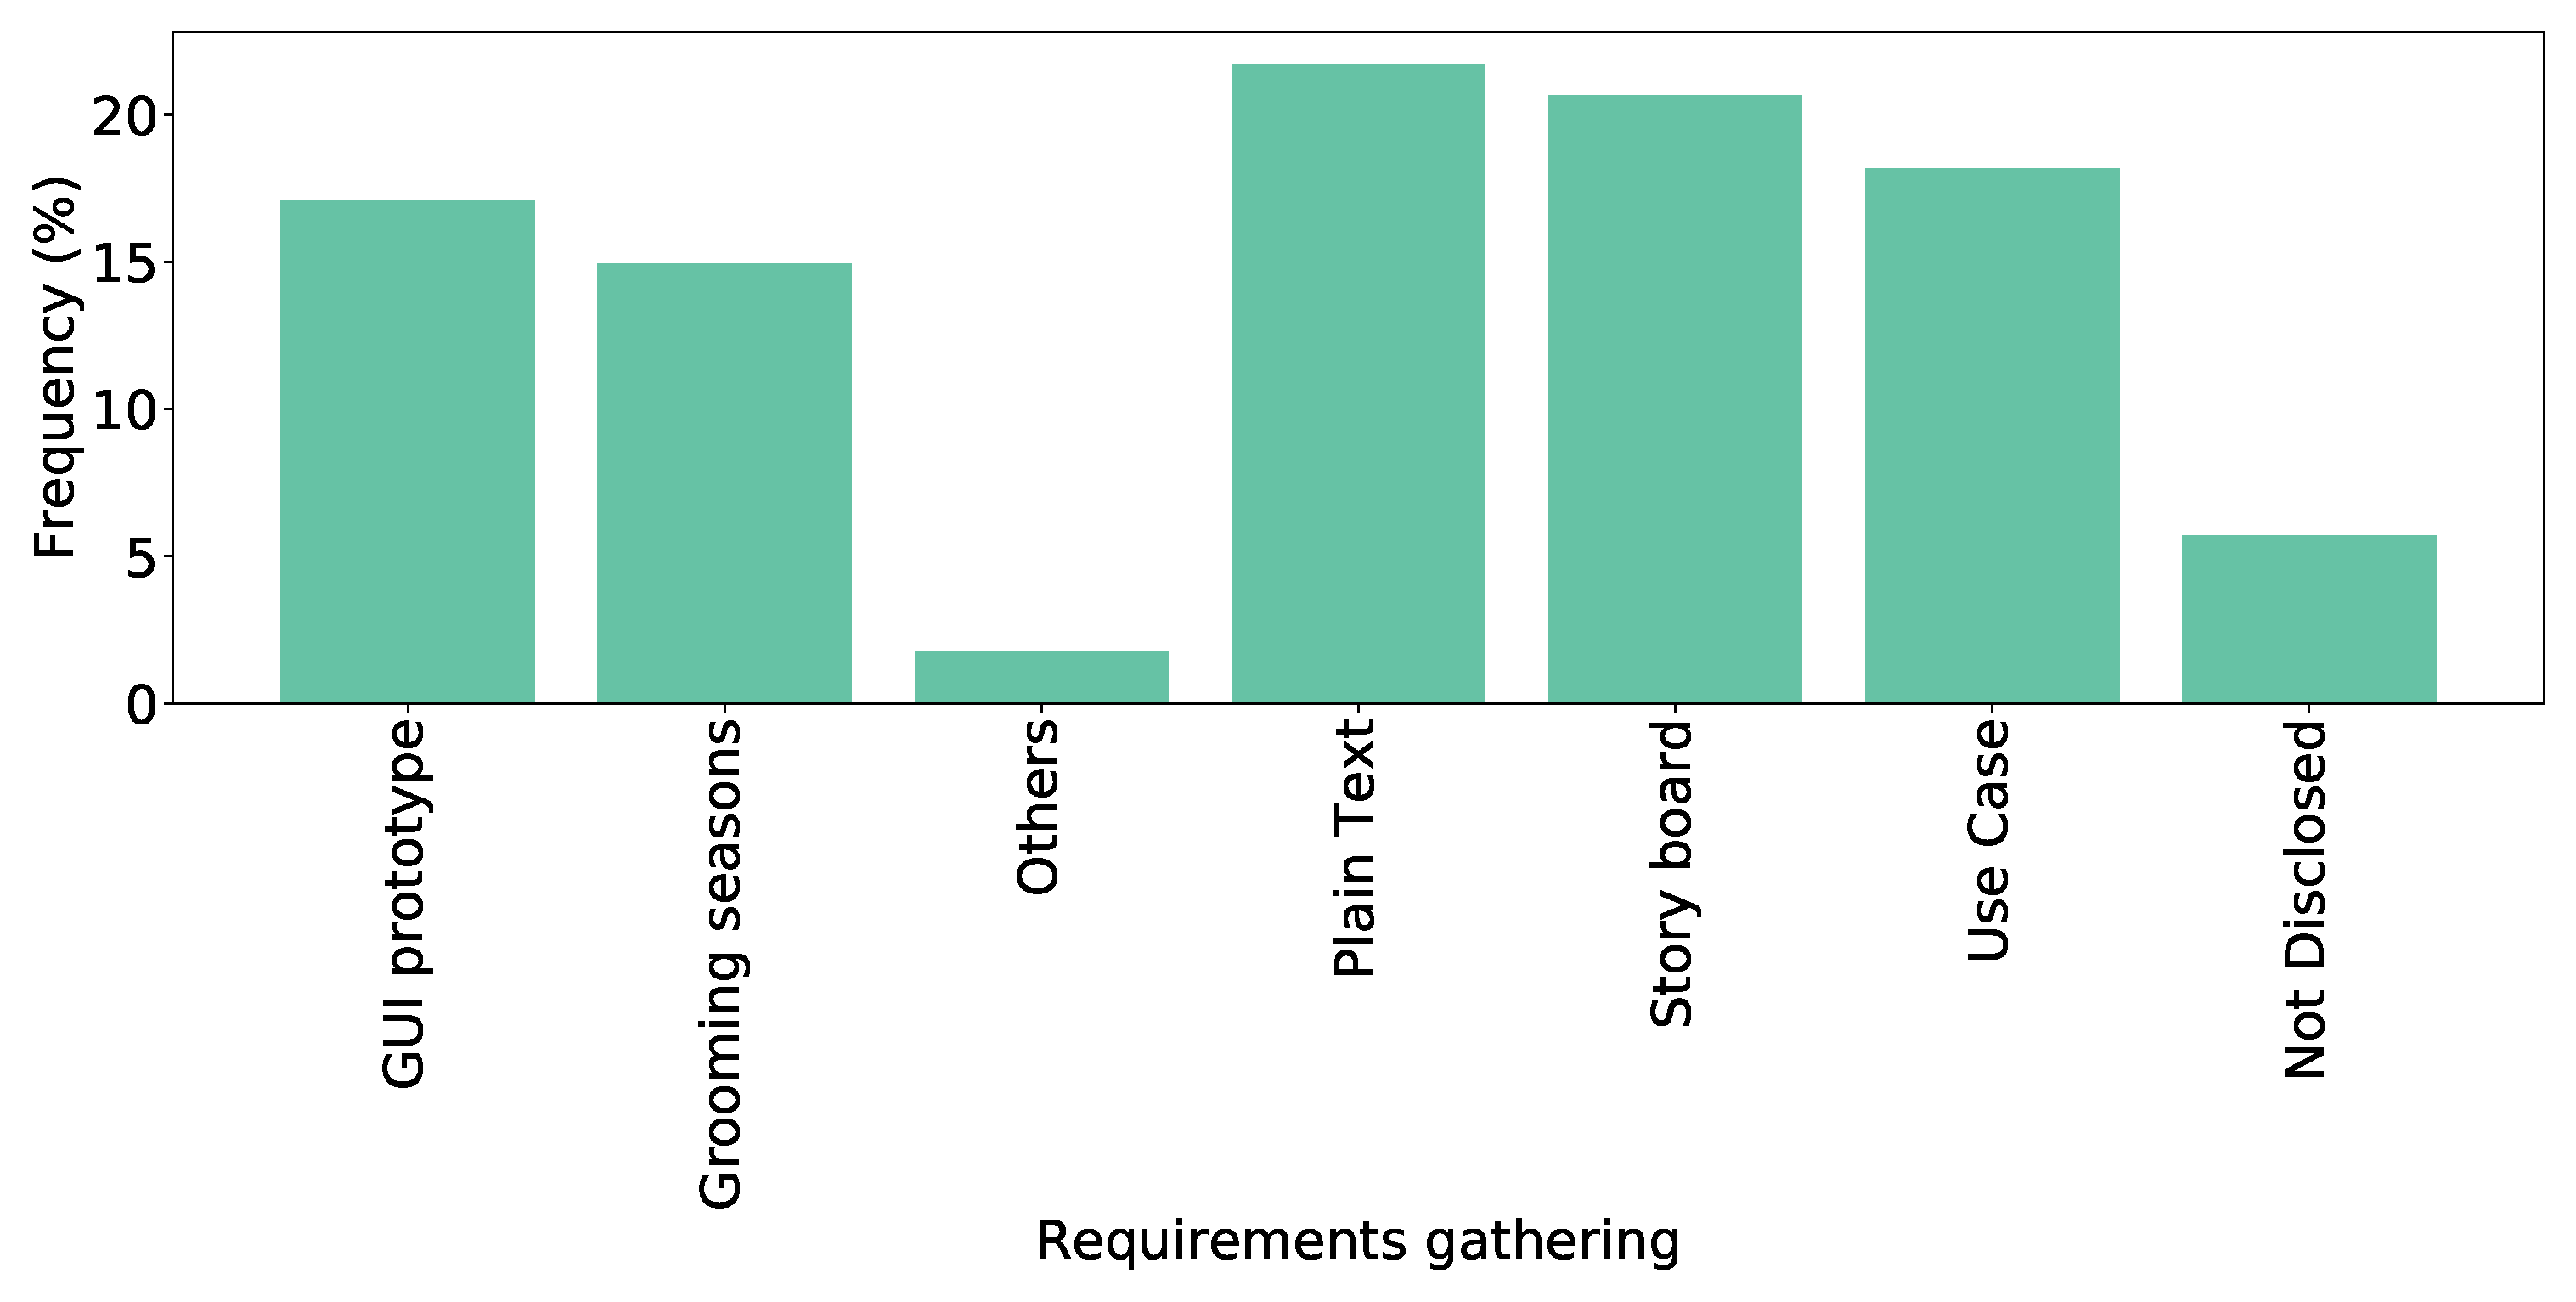
\includegraphics[scale=0.18]{Figures/Requirements_Gathering}
  \caption{Requirements gathering}
  \label{fig:requirements}
\end{figure}


\paragraph{Timeline of Development Activities}
Here, the participants were asked about the most time-consuming software development activities as far as their experience goes. We have presented the activities with respect to the percentage of the participants in Figure \ref{fig:activities}. We see that, according to 65\% of our respondents, most of the time is spent in the implementation stage, whereas the requirement analysis stage requires the second most according to 45\% response. The other usages are program design (37\%), project planning (30\%), testing (19\%), maintenance (17\%), etc.

\begin{figure}[h]
\centering
  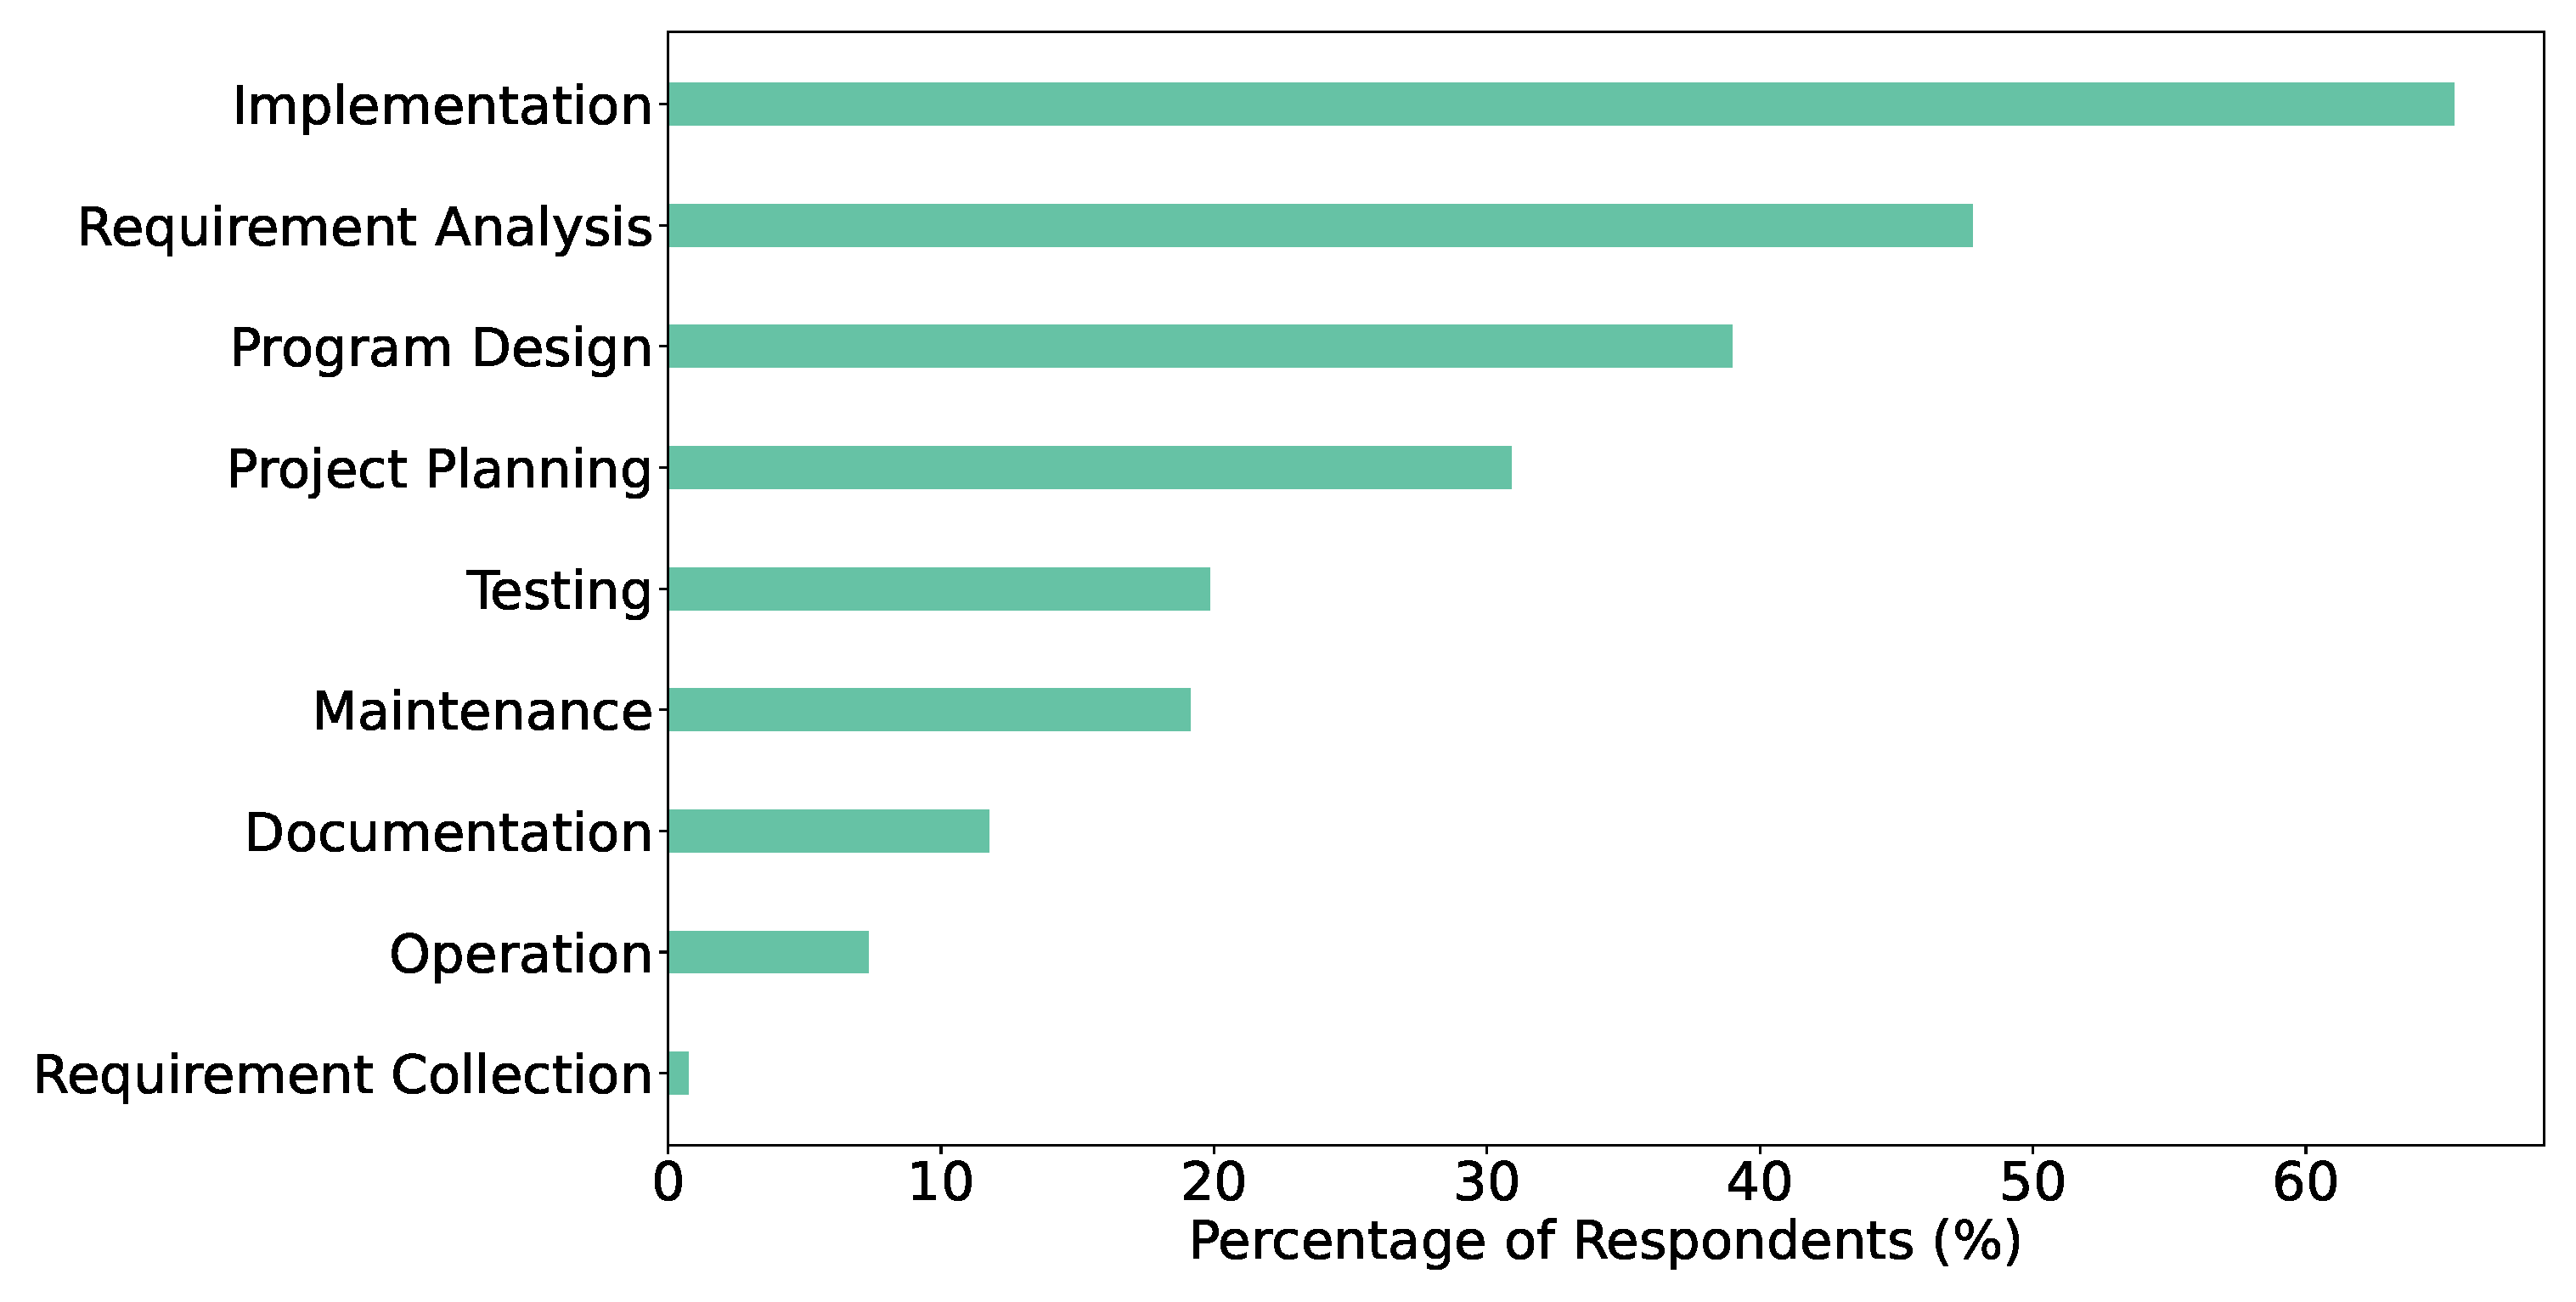
\includegraphics[scale=0.2]{Figures/Respondents_Activities}
  \caption{Software development activities}
  \label{fig:activities}
\end{figure}

We expected that there would be some correlation between software development methodologies (Q6) and the most time-consuming development activities (Q8). Some methodology may add extra time in development activities. \anindya{The previous line does not make clear sense. Can it be rephrased?}\partha{updated}. Thus we have calculated the Cramér`s V \cite{Cramer1946} between the choice of software development methodologies and most time spent activity of the respondents. Cramér`s V calculates the measure of association between two nominal variables\cite{Sheskin2007}. However, we have not found any significant correlation.

\begin{figure}[h]
\centering
  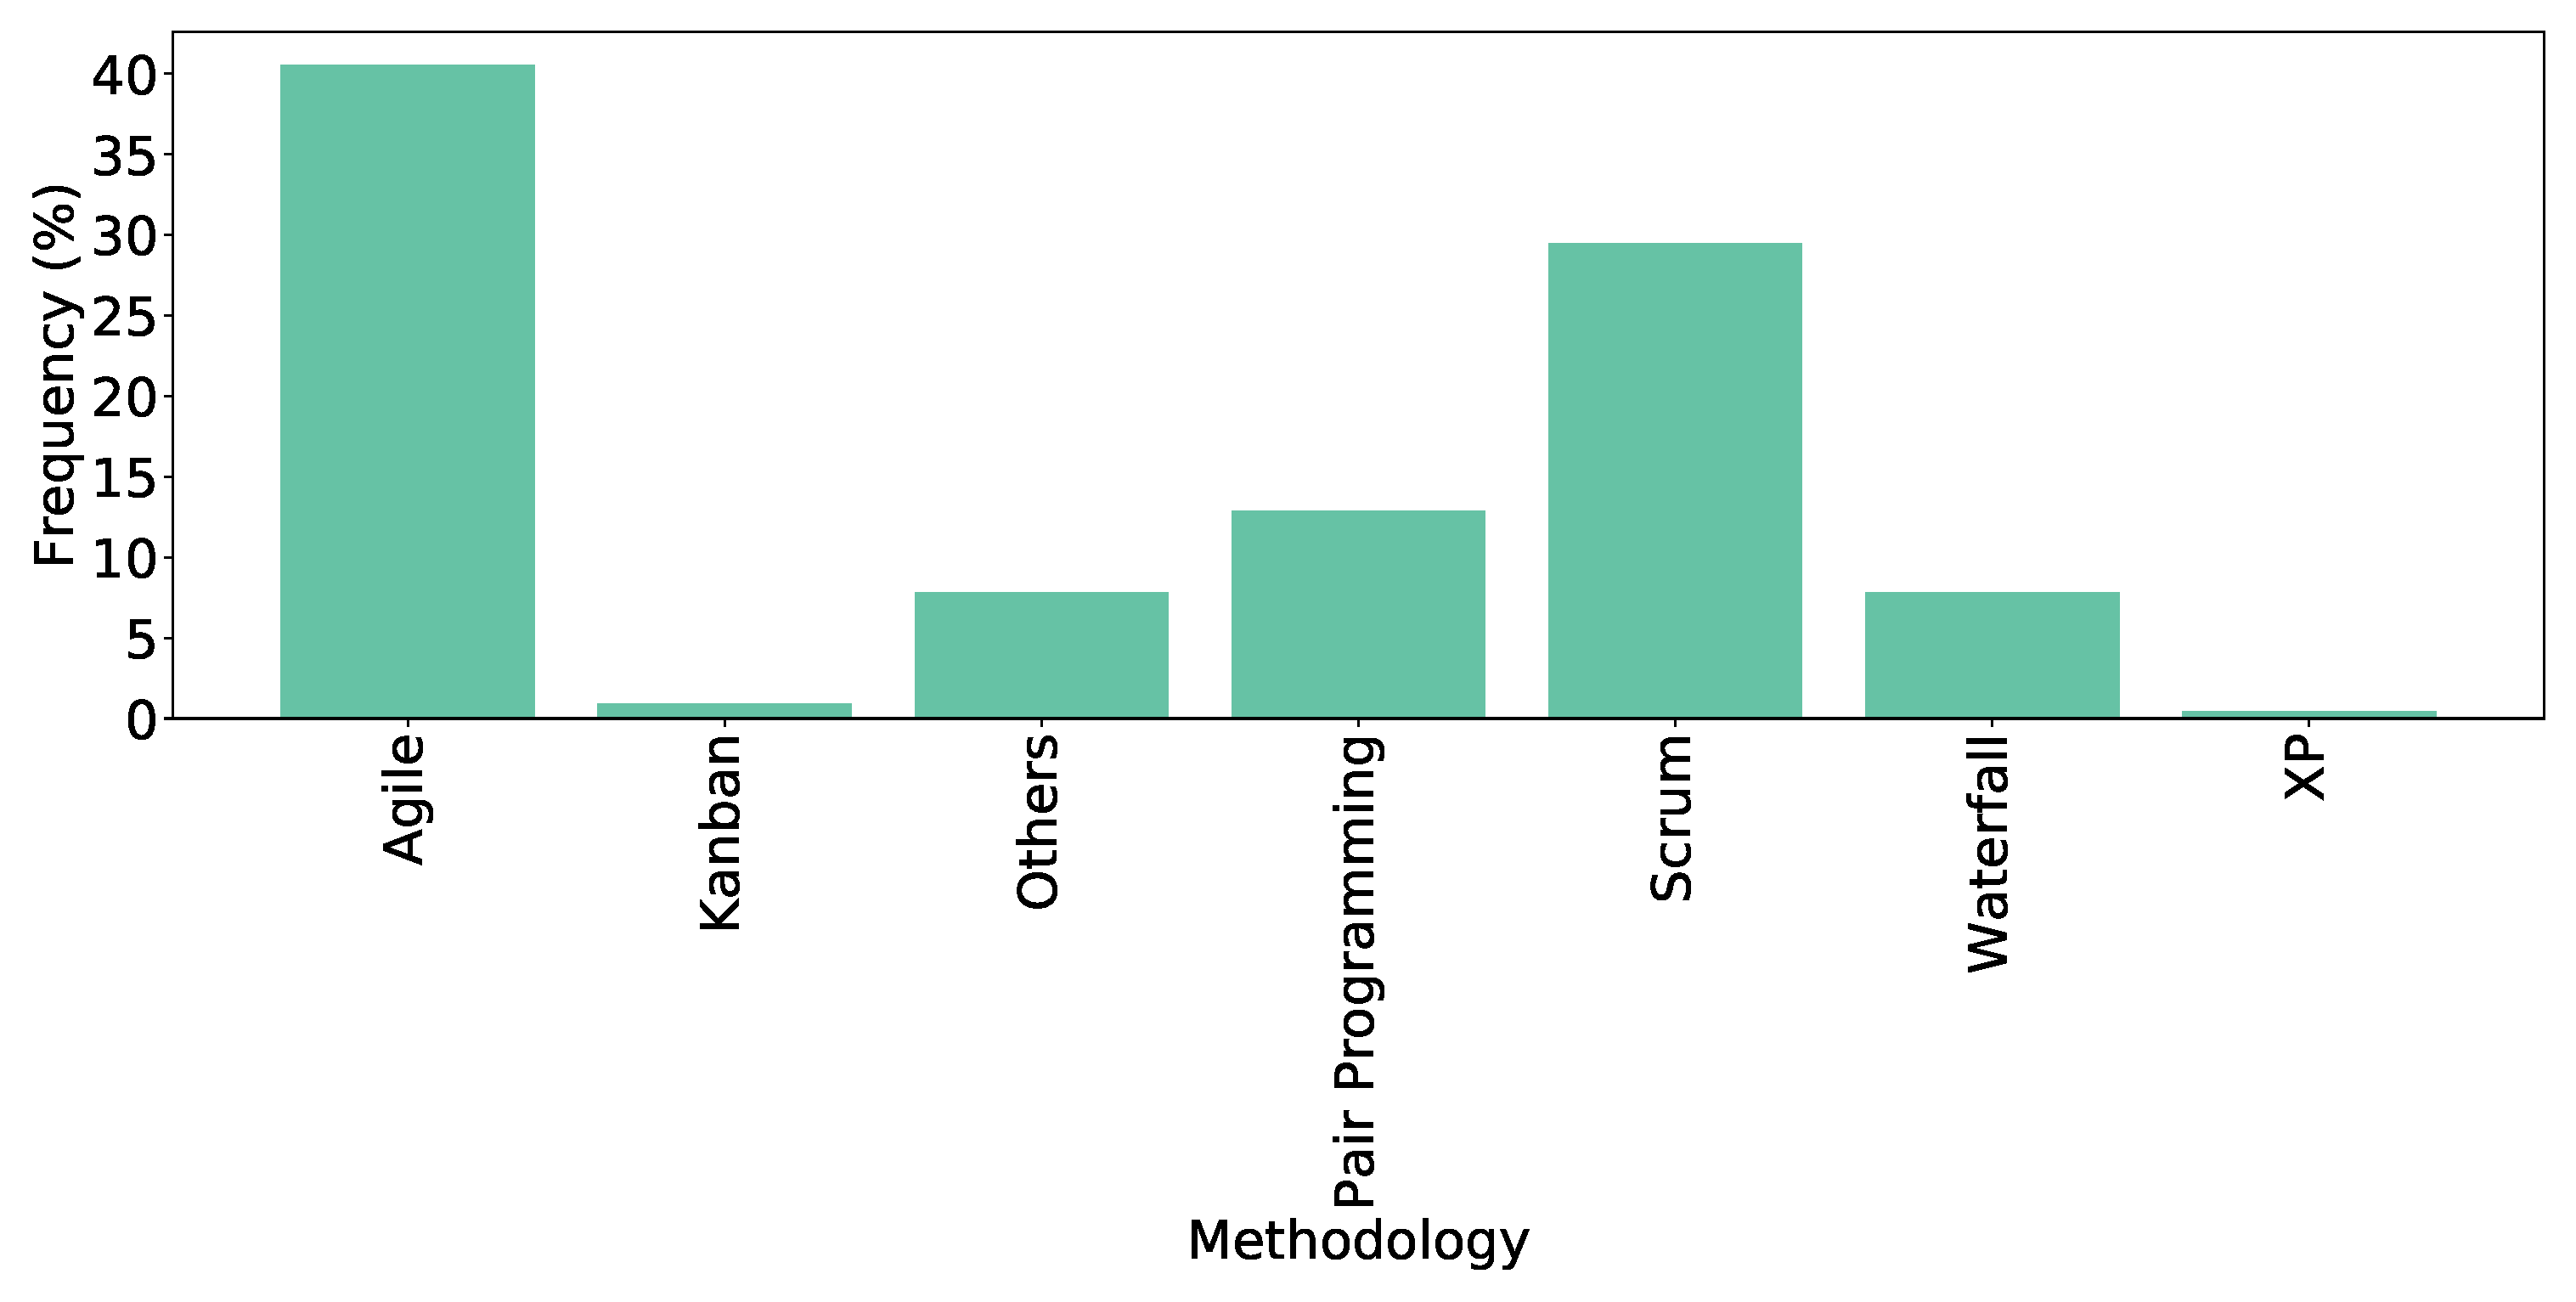
\includegraphics[scale=0.18]{Figures/Respondents_Methodology}
  \caption{Software development methodologies}
  \label{fig:methodologies}
\end{figure}

We guessed that there might be a relation between developers' experience and their activities. It is a general idea that senior developers spend most of their time in requirement specification and design activities, where junior developers spend their time implementing the solution. For analysis purposes, we divided our respondents into two groups based on their professional experience. The two groups are 1) Senior: Developers with more than 5 years of experience 2) Junior: Developers having less than 5 years of experience. We plotted the most time spent activity for the above-mentioned two groups in Figure \ref{fig:activity and seniority}. \anindya{This line is not clear.}\partha{updated}. We can see that our anticipation is right. Junior developers are mostly engaged in the implementation, where senior developers are engaged with requirement specifications.
\anindya{Do you consistently imply coding/development by implementation? In SE, it has a different meaning.}\partha{`Implementation' was one of the options of this closed question. It seems like respondents used it to mean coding/development. One of the responses to another question was `Implementation time carefulness and maintaining a well-developed coding standard.' Though I am not sure, it seems he means coding/development here}

\begin{figure}[h]
\centering
  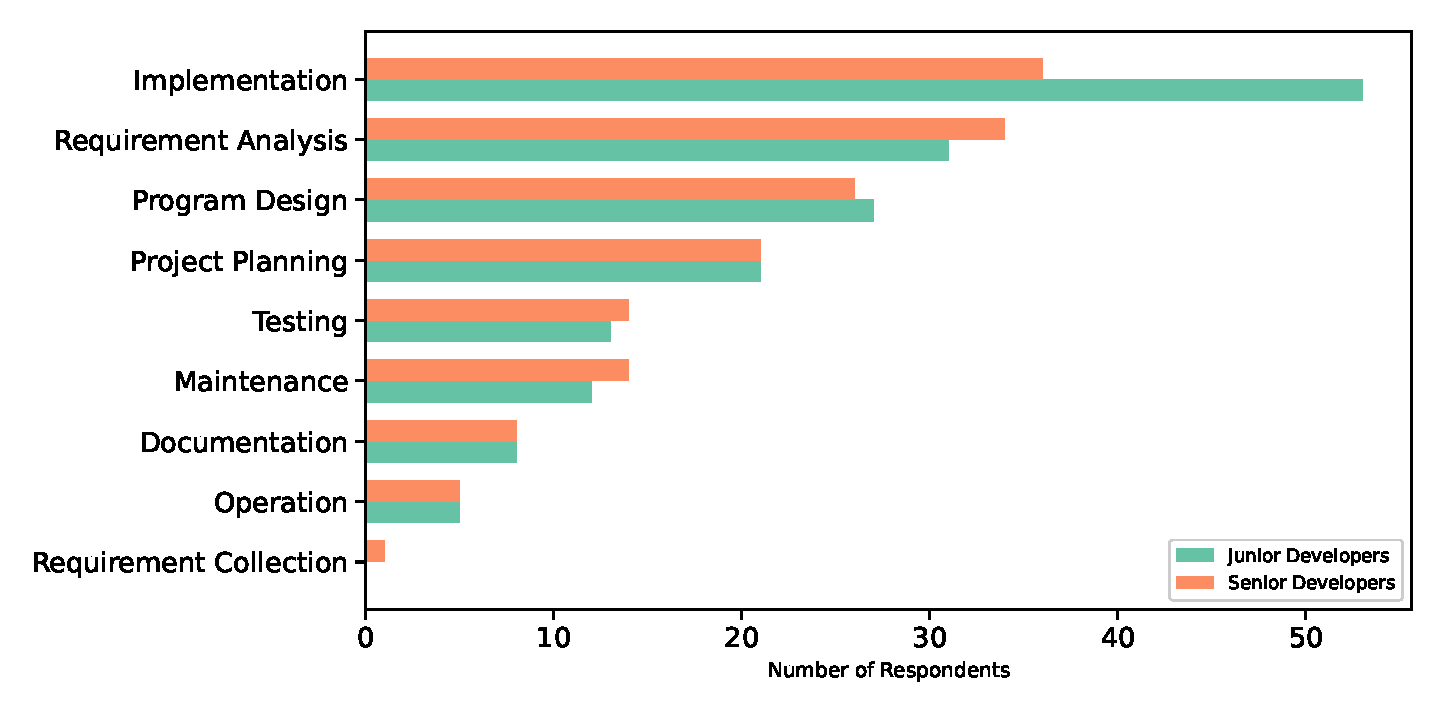
\includegraphics[scale=0.4]{Figures/Activity_and_Seniority.eps}
  \caption{Relation between seniority and activity}
  \label{fig:activity and seniority}
\end{figure}
\partha{In the survey the activity was a multiple choice field. Not sure we can perform any stat. analysis. Will it be theoretically correct?}

\boxtext{Developers of the Bangladeshi SE industry generally spend more time on implementation-related activities than planning and testing.}

\subsubsection{Software development tools and techniques used (D2)}
\label{tools}
%\anindya{Implementation or development??}
We ask five questions related to technologies and tools that are
adopted by software development professionals: \begin{inparaenum}
\item Technology Platform (Q9).
\item Operating System (Q10).
\item Programming Language (Q11).
\item Framework (Q12).
\item IDE (Q13).
\end{inparaenum}

For technology platforms (Q9), most of our survey respondents (80\%) work for the web
platform (Figure \ref{fig:platforms}). The rests are mobile (45\%), desktop (30\%), embedded/IoT
(8\%). This distribution is similar to the 2020 wordwide survey of JetBrains \cite{JetBrains2020}, which finds that 
websites are the
most common type of application developers work on, and the web platform is the
most preferable and popular to develop, followed by desktop and mobile. We have conducted a cross-aspect analysis to identify any relationship
between the technology platform and the requirement gathering process. The
bubble charts in Figure \ref{fig:requirement technology cross analysis}
visualize the cross-aspect analysis. It is clear from the figure that the
requirement gathering process is mostly practiced in GUI-based development
(e.g., web, desktop, mobile).
\begin{figure}[t]
\centering
  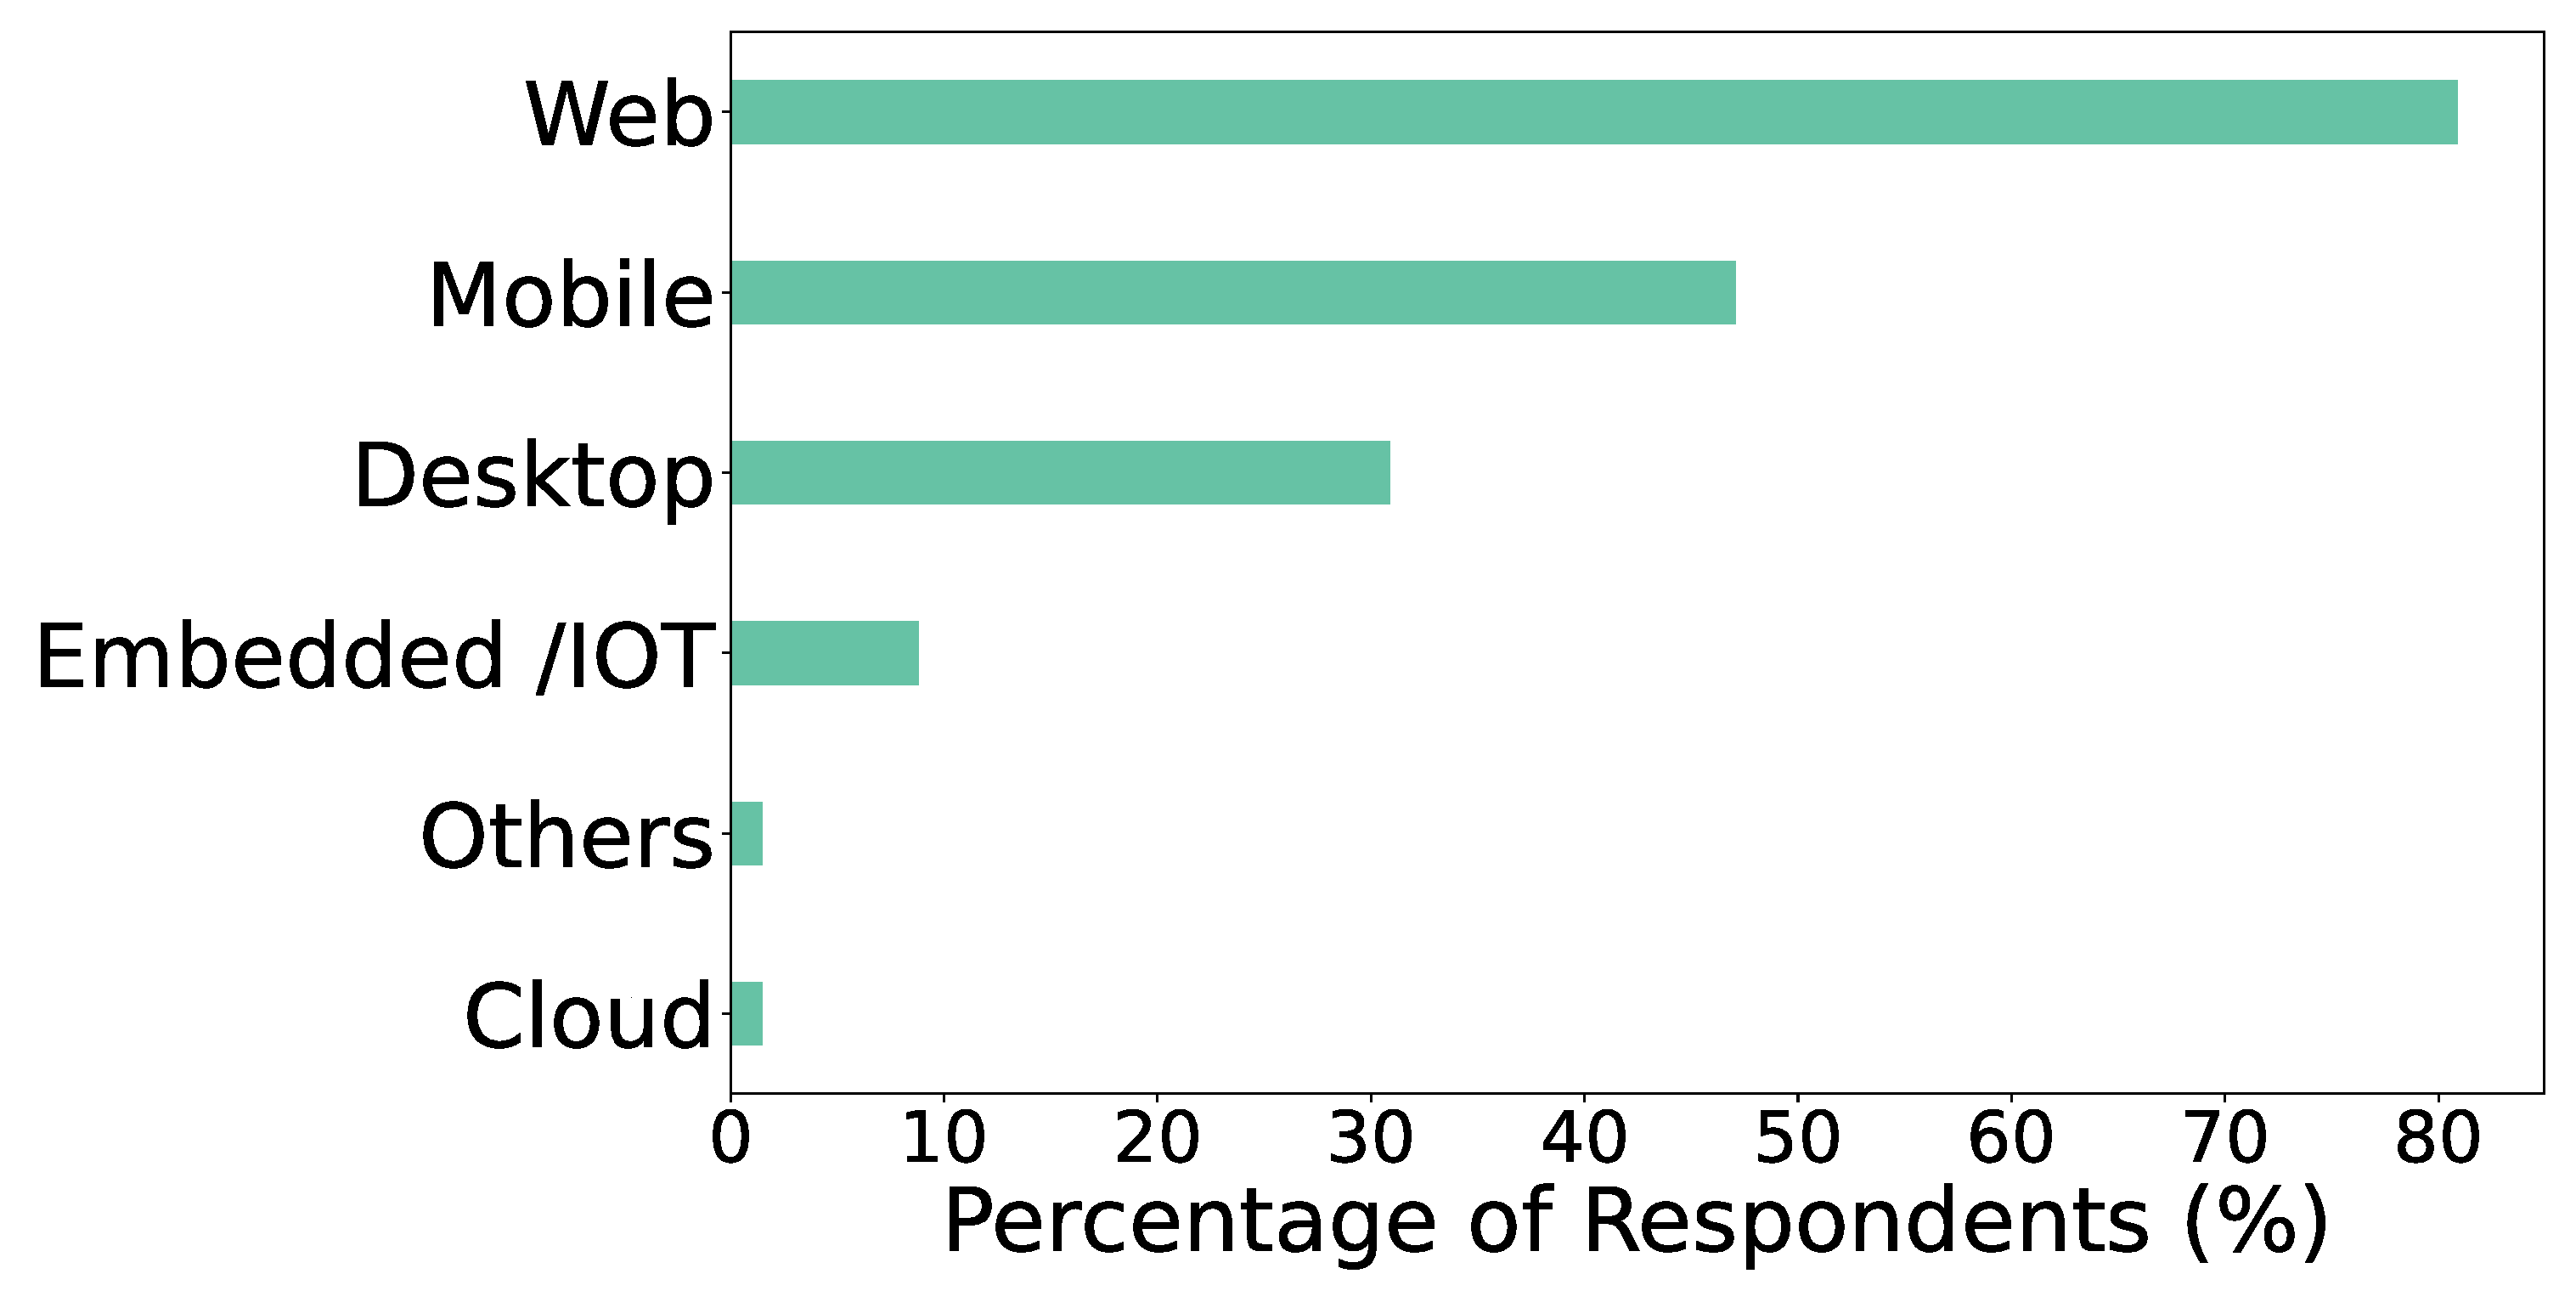
\includegraphics[scale=0.18]{Figures/Respondents_Technologies}
  \caption{Technology Platforms}
  \label{fig:platforms}
\end{figure}
\begin{figure}[t]
\centering
  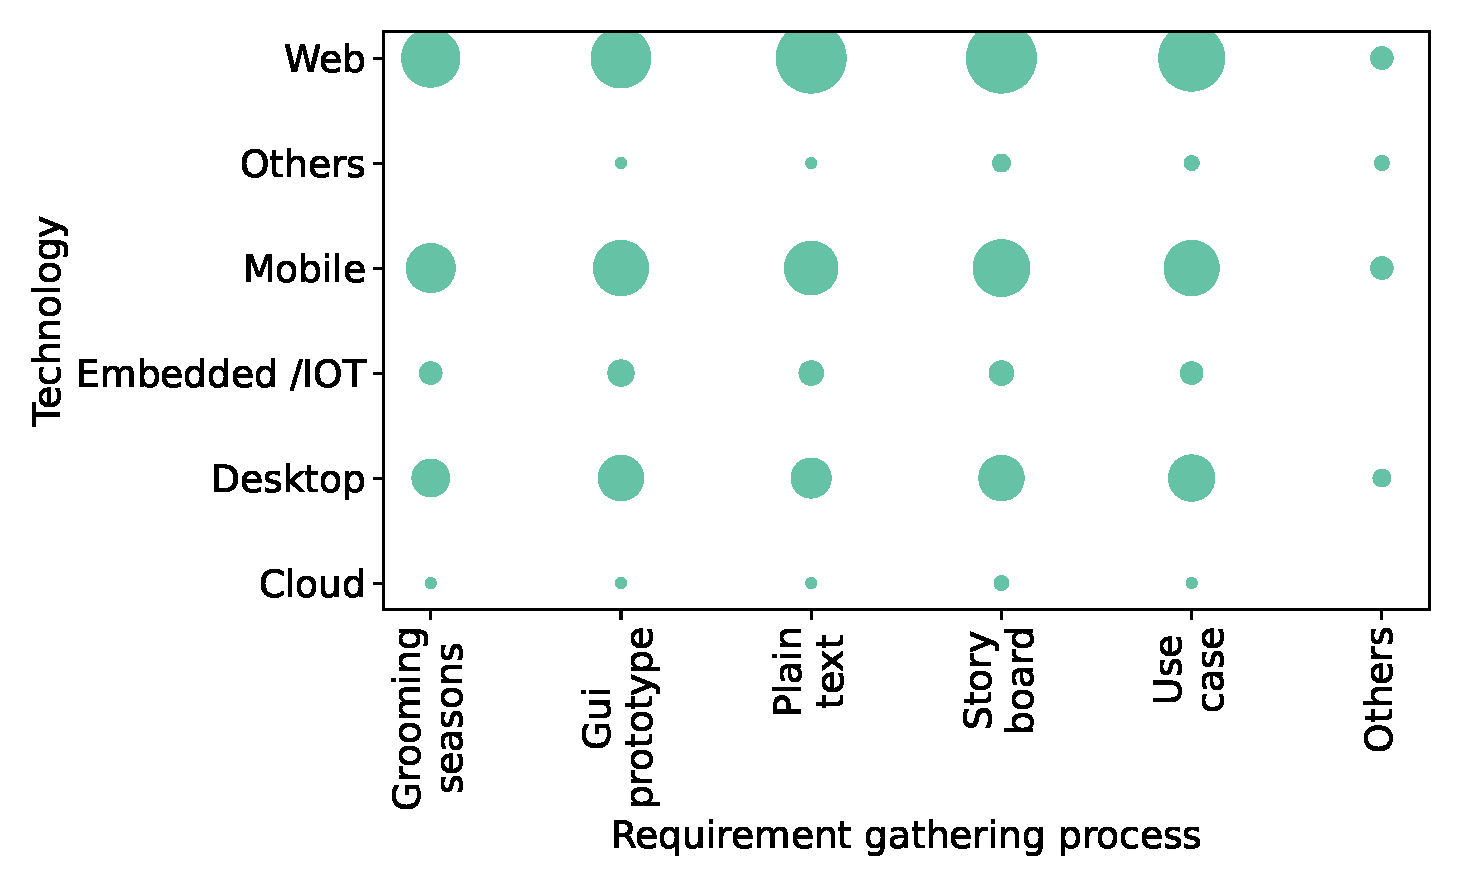
\includegraphics[scale=0.47]{Figures/Requirement_Technology_Cross_Analysis.eps}
  \caption{Cross aspect analysis of requirement gathering and technology platform}
  \label{fig:requirement technology cross analysis}
\end{figure}

%\paragraph{Operating Systems (Q10).} 

For operating systems (Q10), most of our
respondents preferred Linux based operating system (56\%) for their development (Figure \ref{fig:os}). The second frequently used
operating system is Windows (45\%) followed by MacOS (28\%). We
observed similar scenarios in the 2018 and 2019 StackOverflow (SO) surveys
\cite{StackoverflowSurvey2018,StackoverflowSurvey2019}. However, Windows ranked
first in the 2020 survey of both SO and JetBrains \cite{StackoverflowSurvey2020,
JetBrains2020}. The recent higher preference towards Windows could be due to the newly
included WSL (Windows Subsystem for Linux). This feature allows users to perform
almost any Linux-specific task on Windows. We anticipated that the use of OS
might be related to professional experience. Among the participants,
senior/expert developers (those with at least 5 years of experience) have significantly higher rates of Linux usage ($p=0.024$ based on Mann Whitney U test). 
\begin{figure}[h]
\centering
  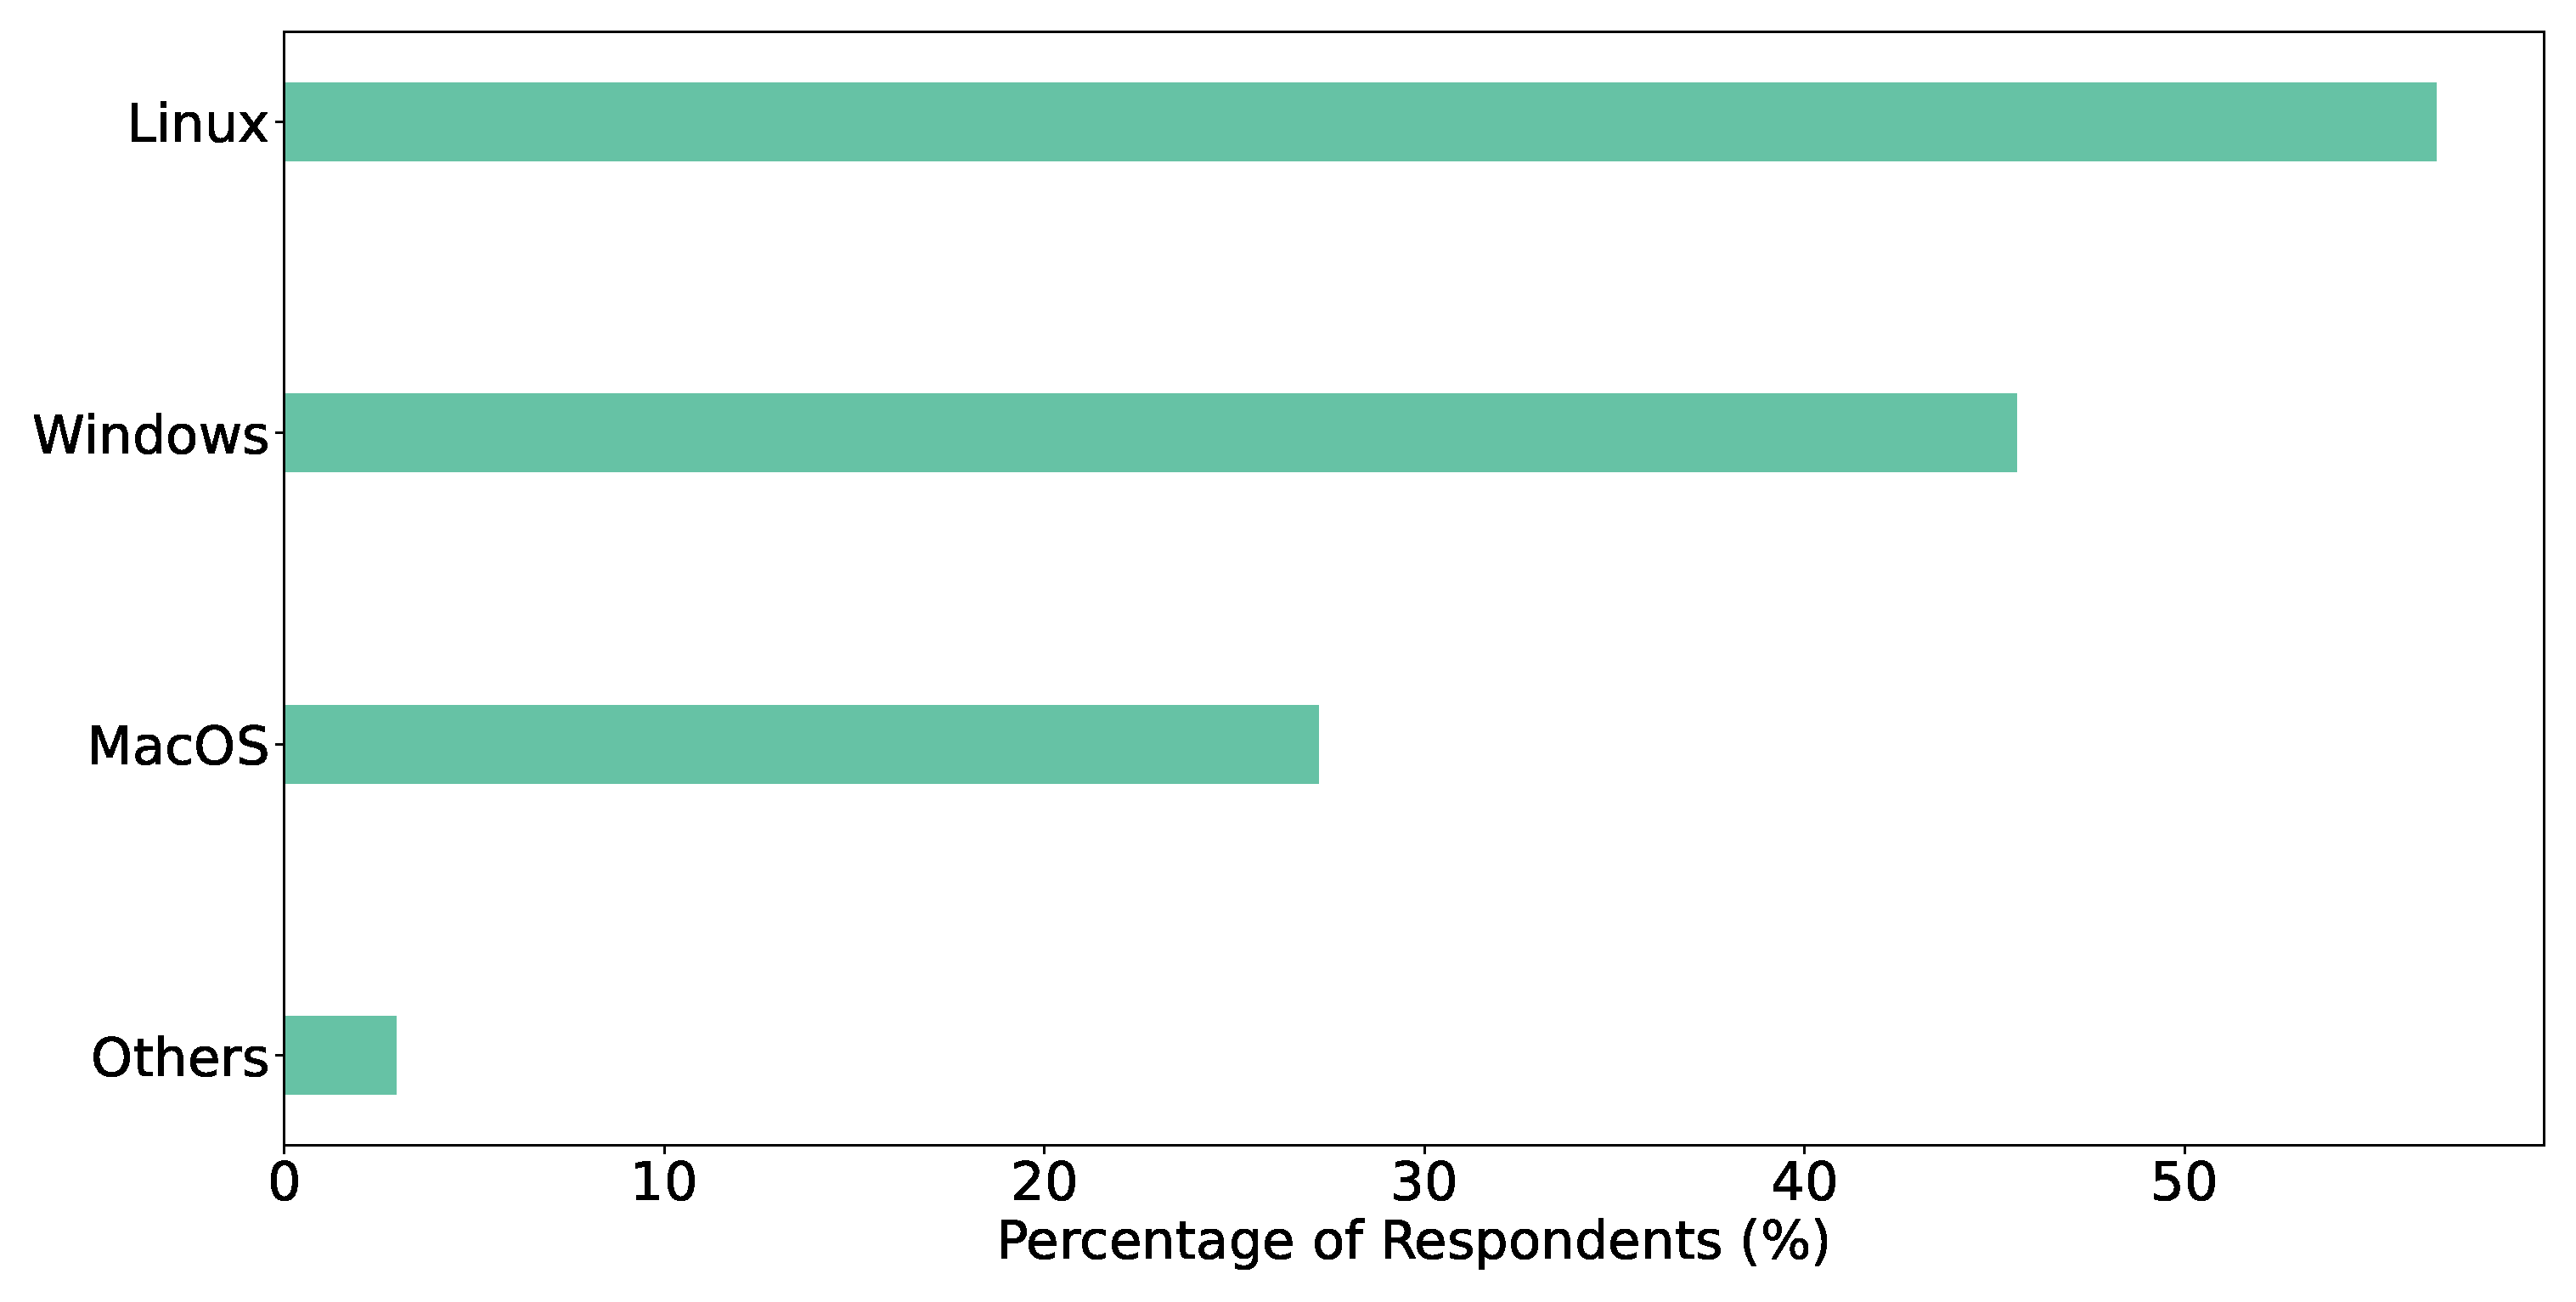
\includegraphics[scale=0.17]{Figures/Respondents_os}
  \caption{Operating Systems}
  \label{fig:os}
\end{figure}
%\paragraph{Programming Languages (Q11).} 
For programming languages (Q11), around 65\% and 60\% of our respondents use JavaScript and
Java, respectively, which are the two most used languages in Bangladesh (Figure
\ref{fig:languages}). Both JavaScript and Java are popular for web and mobile
platforms. A great percentage of our survey participants develop for both
web and mobile platforms. Other languages
like PHP (25\%), Python (25\%), and C\# (18\%) are also used, which indicates
that the software engineers are not biased towards a single specific language.
Our survey result matches with the last two years' Stack Overflow survey and the
GitHub stat. In all of the cases, JavaScript is the most used language, followed
by Java and Python \cite{StackoverflowSurvey2020, StackoverflowSurvey2019,
GithubStat}. We
observed that users using mobile and web platforms mostly use Java and
Javascript as programming languages. However, this is not statistically
significant ($p=0.1$). Though the use of the operating system can be influenced by
programming language (e.g., Swift and macOS), we do not find any significant correlation
between the two choices.
\begin{figure}[t]
\centering
  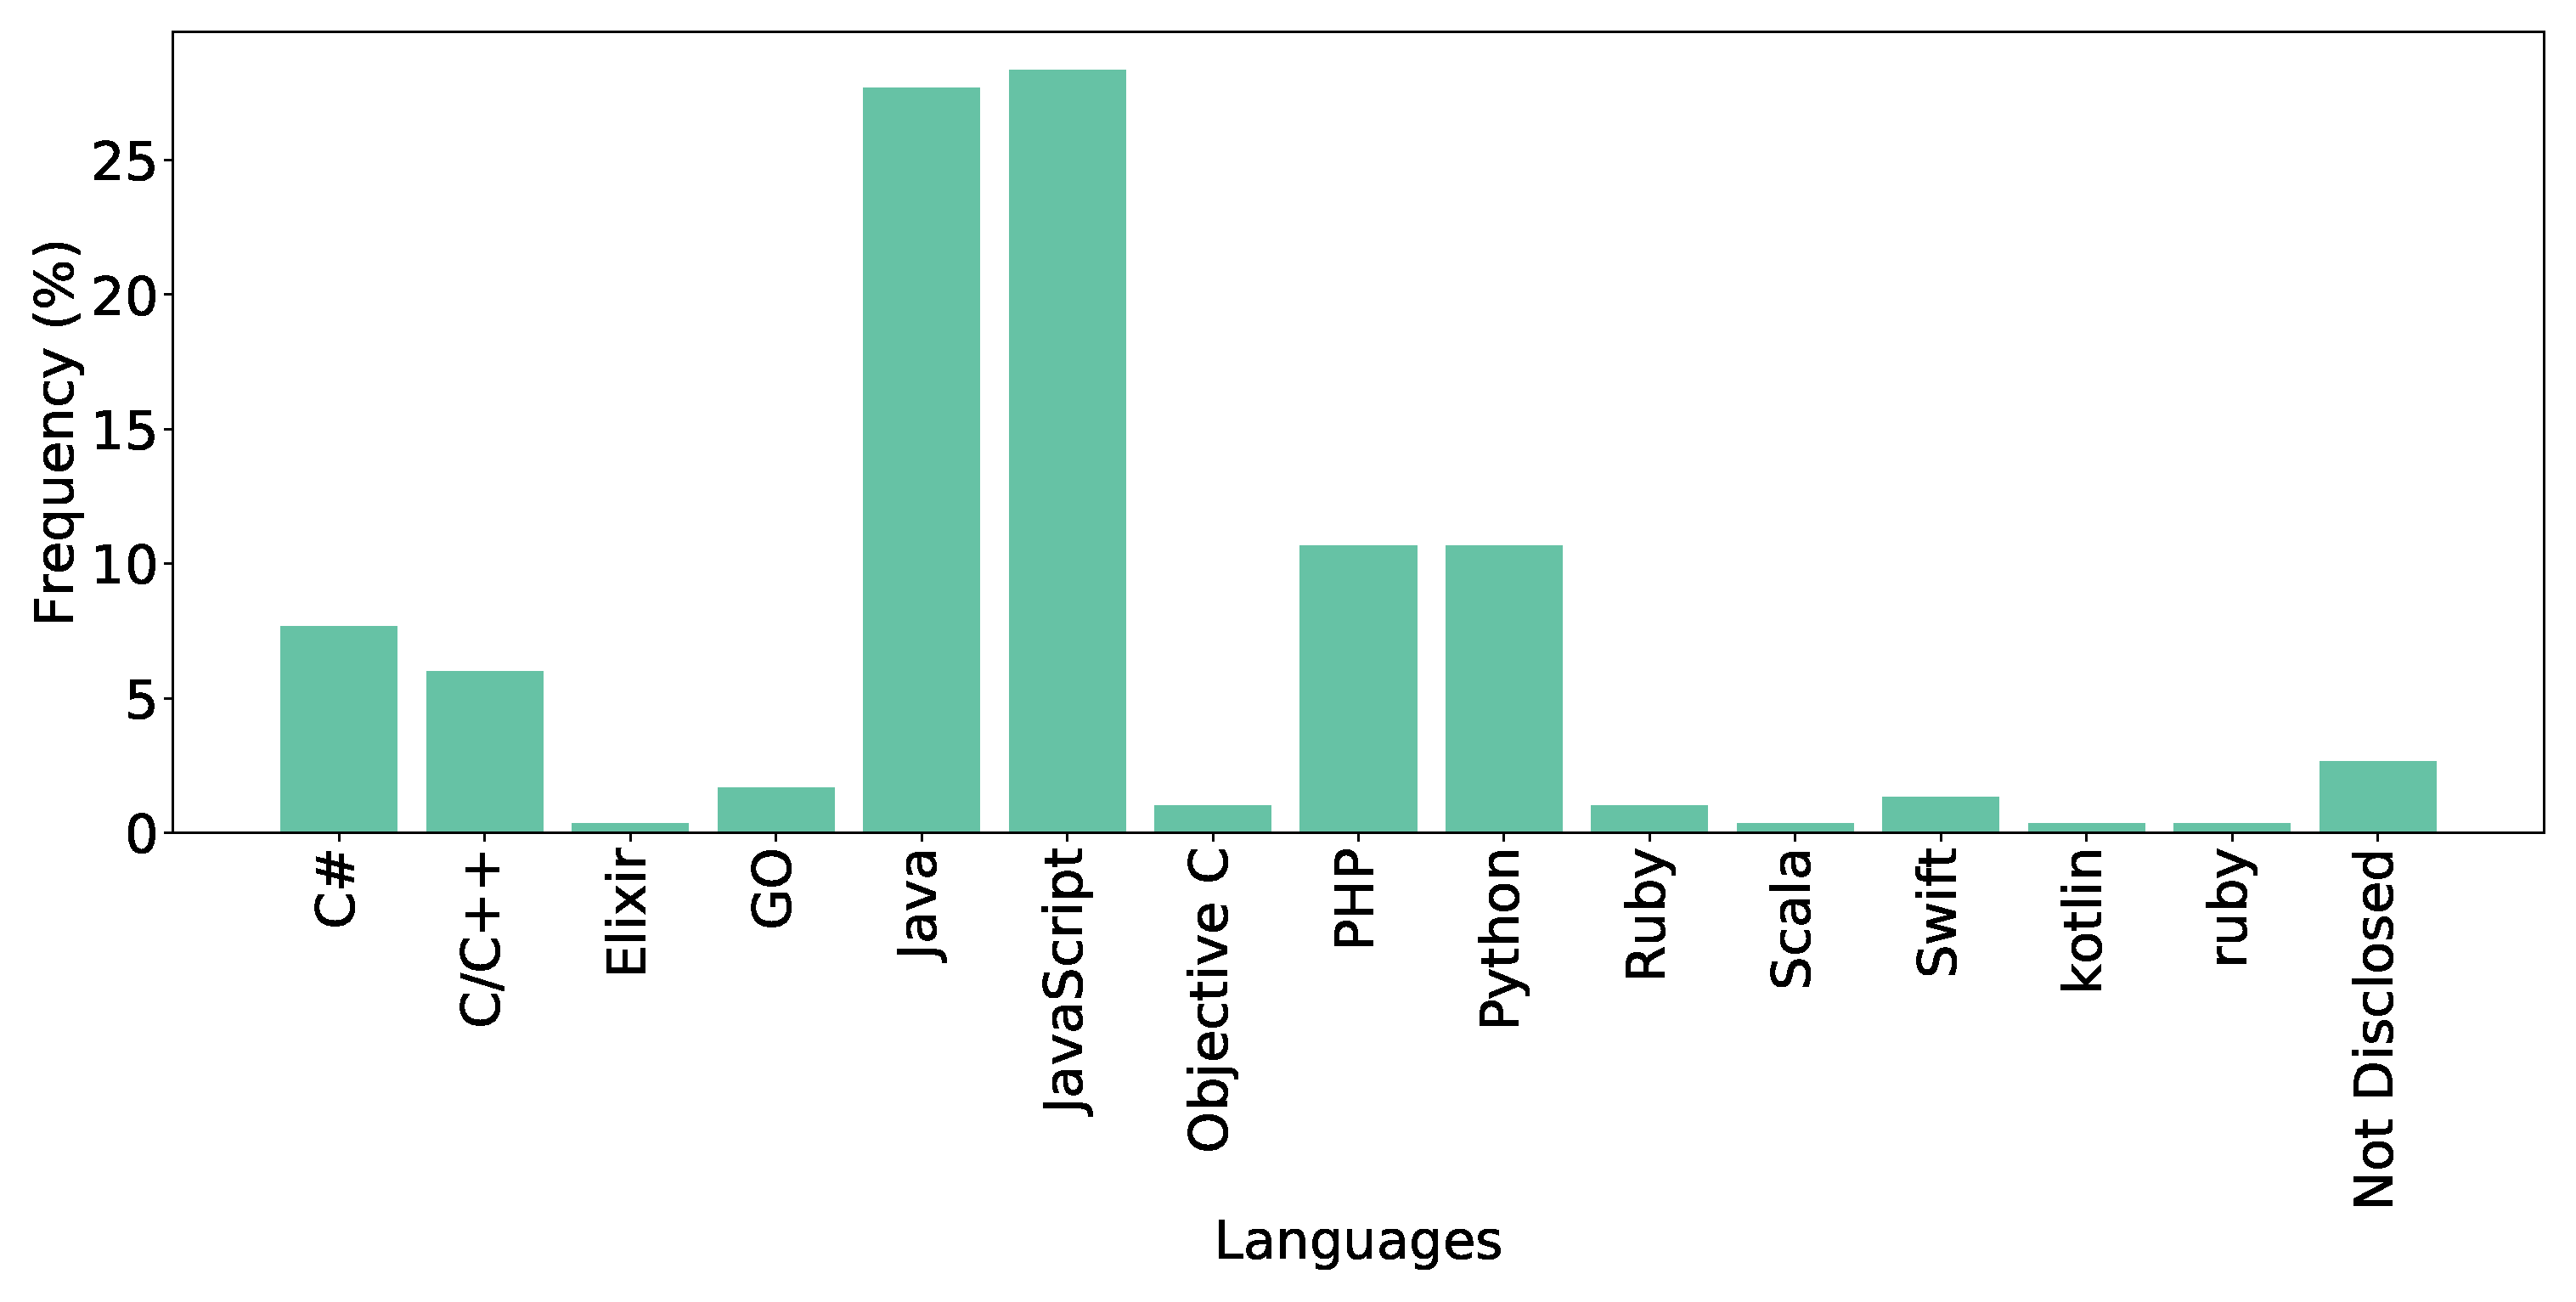
\includegraphics[scale=0.18]{Figures/Respondents_languages}
  \caption{Languages used in software development}
  \label{fig:languages}
\end{figure}

%\paragraph{Frameworks used in development}
For frameworkes used in development (Q12), as shown in Figure \ref{fig:frameworks} Spring boot (37\%) is the most used framework in the Bangladesh software industry. 
This observation is aligned with the result of Java's usage rate corresponding
to Figure \ref{fig:languages}. Since JavaScript is the most used language of our
respondents, they use various JavaScript frameworks such as React, Node.js,
Angular, Express, etc. ASP.NET, Django, and
Laravel are used in the same proportion based on around 15\% of our respondents.
React, Swift, Ruby on Rails, Node.js, etc., are comparatively less used. Other
than these, lots of frameworks such as Cocoa, Meteor, TestNG, Relay, Appium,
CakePHP, etc., are also used (presented as `Others' in Figure \ref{fig:frameworks}). For web development, Django
and Spring frameworks are mostly used in Bangladesh ($p=0.04$). We have compared
our results with the Stack Overflow 2016 to 2020
survey\cite{StackoverflowSurvey2017, StackoverflowSurvey2018,
StackoverflowSurvey2019, StackoverflowSurvey2020}. The only common framework in
the top five list in both surveys is ASP.NET. In the stack overflow survey, we
noticed that JavaScript-based frameworks (e.g., Jacqueline, Angular, React,
Node.js) occupy the top positions (top five), which is not the case for our
survey.

\begin{figure}[t]
\centering
  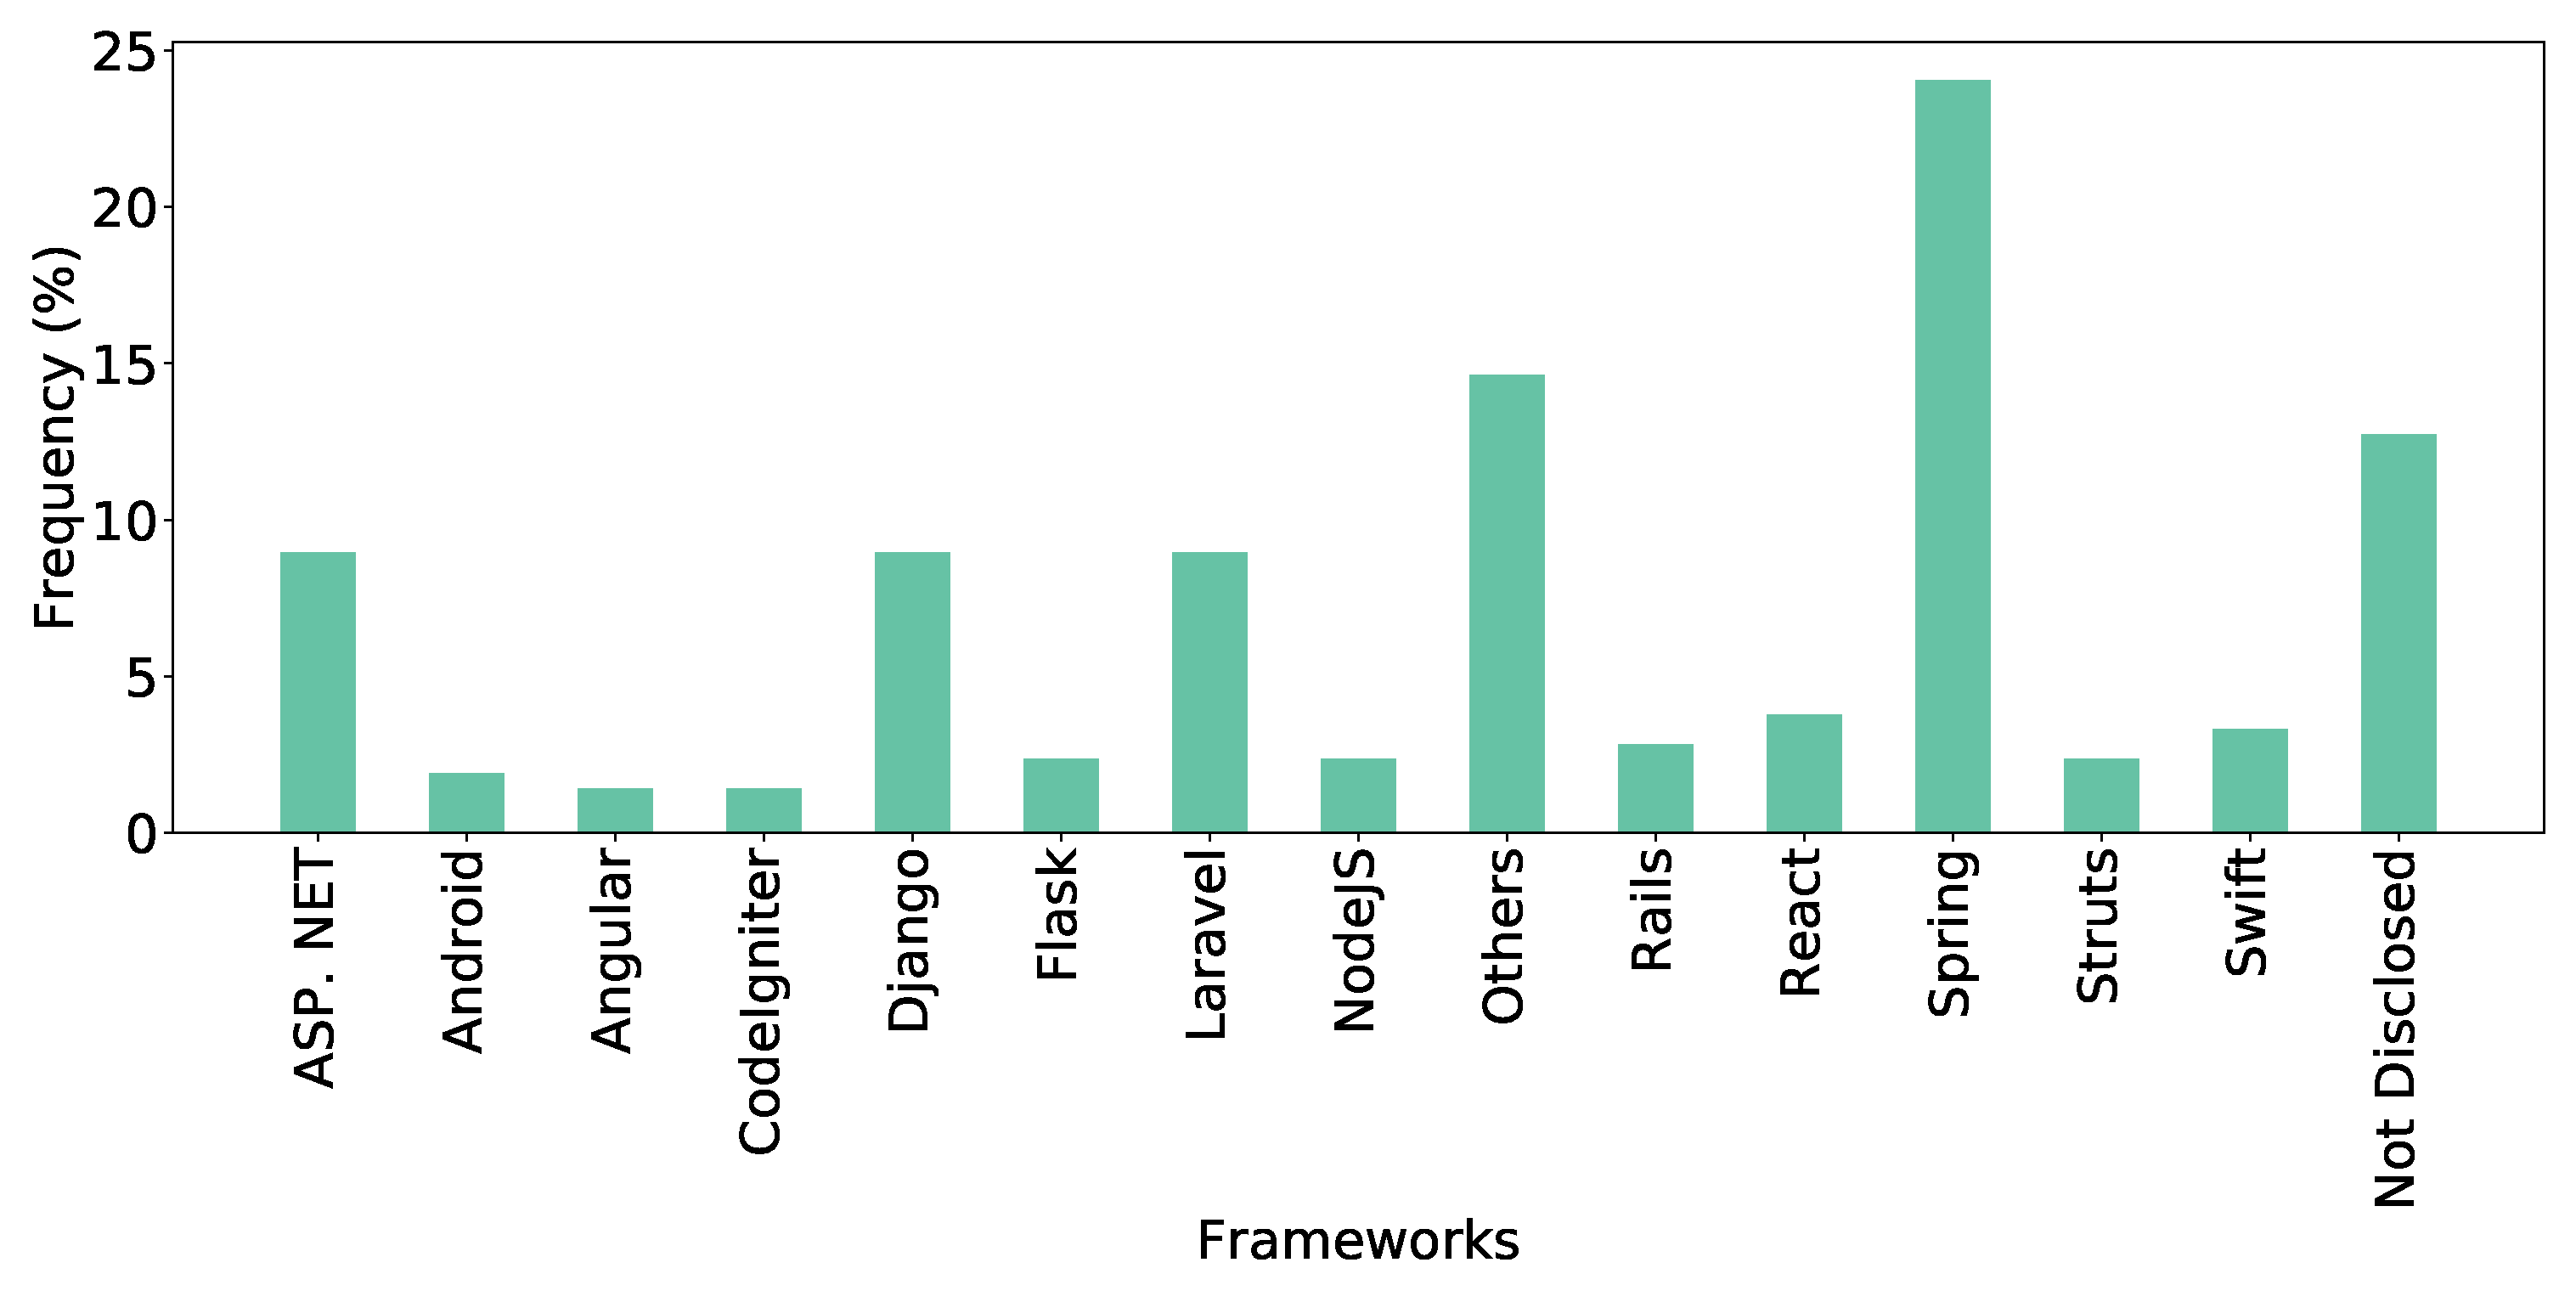
\includegraphics[scale=0.18]{Figures/Respondents_frameworks}
  \caption{Frameworks}
  \label{fig:frameworks}
\end{figure}

%\paragraph{IDE's used by the respondent's} 
Among the IDEs (Q13), as shown in Figure \ref{fig:IDEs},
IntelliJ, is used by most respondents (43\%). IntelliJ is a Java integrated development tool for developing software for the
enterprise, mobile, and web application, The
other IDEs used in SE industries are Visual Studio (30\%), Eclipse (24\%),
PyCharm (17\%), NetBeans (11\%), and Android Studio (7\%).

\begin{figure}[t]
\centering
  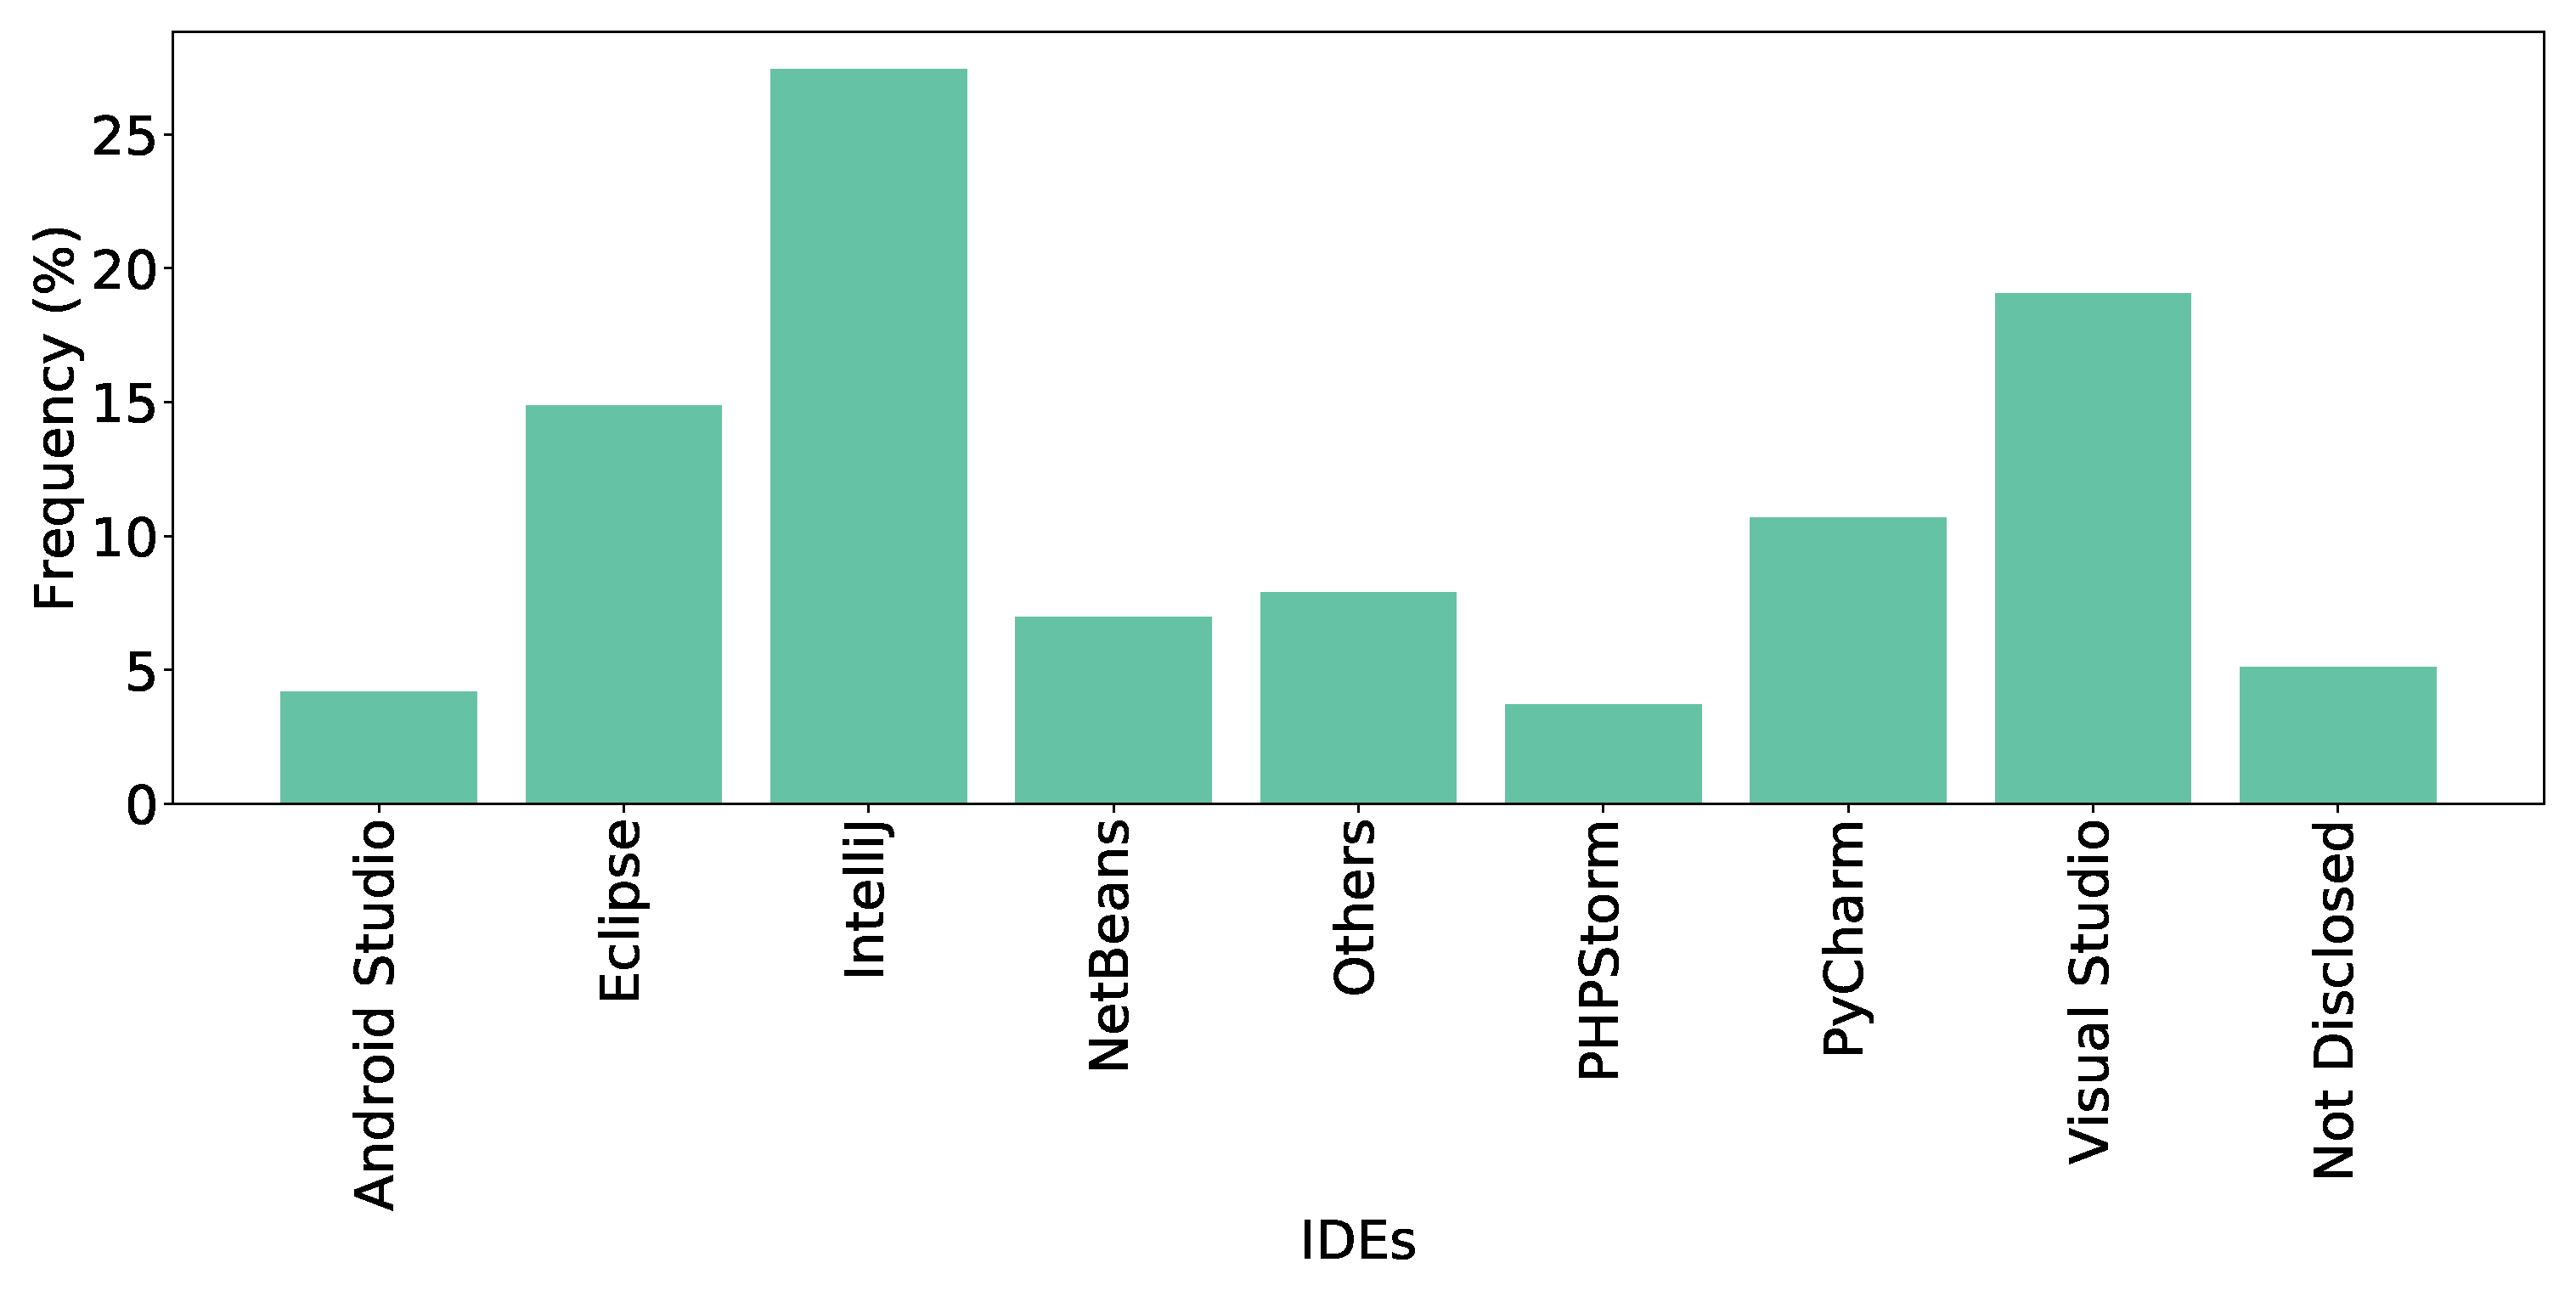
\includegraphics[scale=0.18]{Figures/Respondents_IDEs}
  \caption{IDE's}
  \label{fig:IDEs}
\end{figure}
\begin{tcolorbox}[flushleft upper,boxrule=1pt,arc=0pt,left=0pt,right=0pt,top=0pt,bottom=0pt,colback=white,after=\ignorespacesafterend\par\noindent]
\nd\it{\bf{RQ1-D2. Software development tools and techniques used.}} Web based software services top the list of development technologies. Requirement gathering process is mostly practiced in GUI-based development
(e.g., web, desktop, mobile) \gias{summarize findings from Q10-13 also here}
\end{tcolorbox}
% \boxtext{Web based software services top the list of development technologies. Requirement gathering process is mostly practiced in GUI-based development
% (e.g., web, desktop, mobile) \gias{summarize findings from Q10-13 also here}}

\subsubsection{What type of testing and deployment practices are used?}
\label{testing_practices}

Testing is an important process in improving the quality of the software product. The purpose of this process is to find errors, which might occur during specification, design, and code generation. We report the following results next:
\begin{itemize}
\item Software Testing Practices (Q 14)
\item Level of Automated Testing (Q 15)
\item Tools Used in Testing and QA (Q 16)
\item Continuous Deployment tools (Q 17)
\item Version Control (Q 18)
\end{itemize}


\paragraph{Software Testing Practices}
According to Figure \ref{fig:testing}, several numbers of testing practices are used during software development. The results show that most of the organizations have carried out unit testing (53\%), functional testing (49\%), user acceptance testing (39\%), GUI testing (31\%), etc. Unit testing also ranked first in the 2019 survey of JetBrains, where it was voted by 71\% participants across the globe \cite{JetBrains2019}. We observed in our survey that in some cases managers have reported to perform GUI testing and performance testing, which is unlikely due to their role/designation. However, the observation is not statistically significant ($p=0.12$). It may be deduced that in absence of enough specialized resource managers have to take additional responsibility. To identify the relation between testing practices and experience, we plotted them together in Figure \ref{fig:testing type and experience}. In Figure \ref{fig:testing type and experience}, we observed that junior developers mostly perform unit, integration, and functional testing, whereas senior developers mostly perform API testing. We conducted the Mann Whitney U test to assess the conjecture, and it is found statistically significant ($p$<$0.01$).
\begin{figure}[h]
\centering
  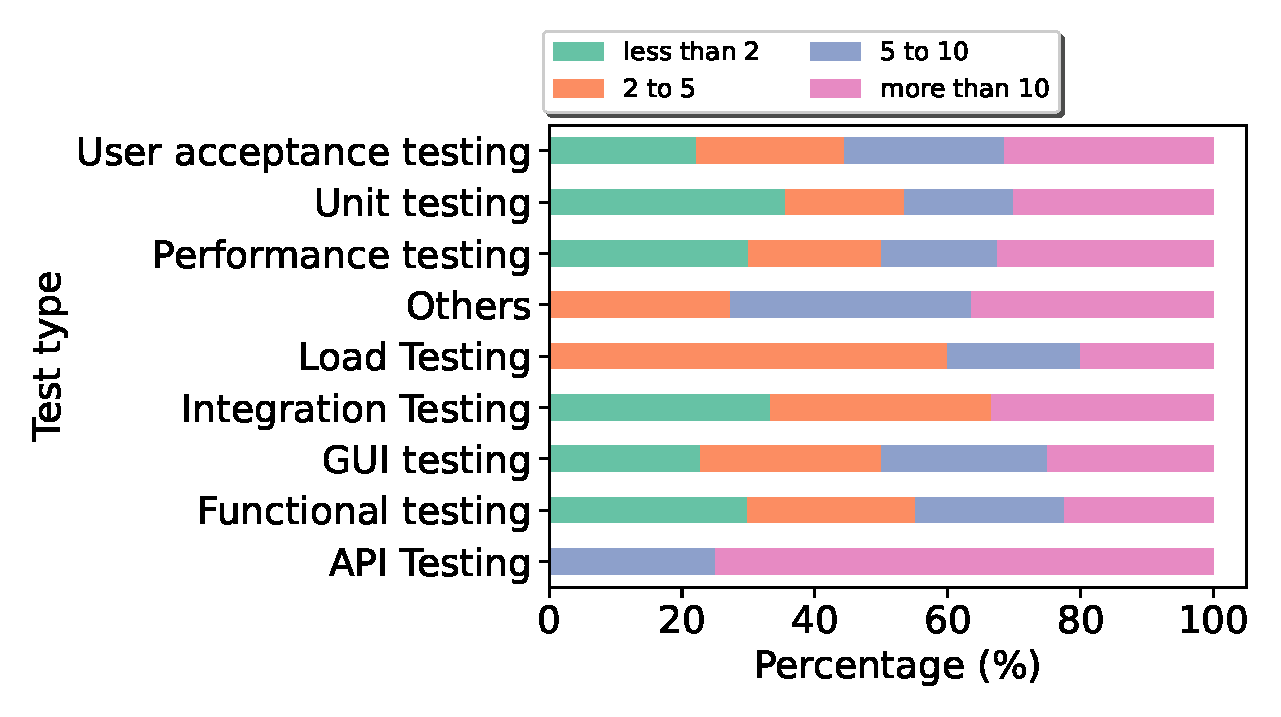
\includegraphics[scale=0.6]{Figures/Testing_Type_and_Experience}
  \caption{Testing practices ans professional experience}
  \label{fig:testing type and experience}
\end{figure}

\begin{figure}[h]
\centering
  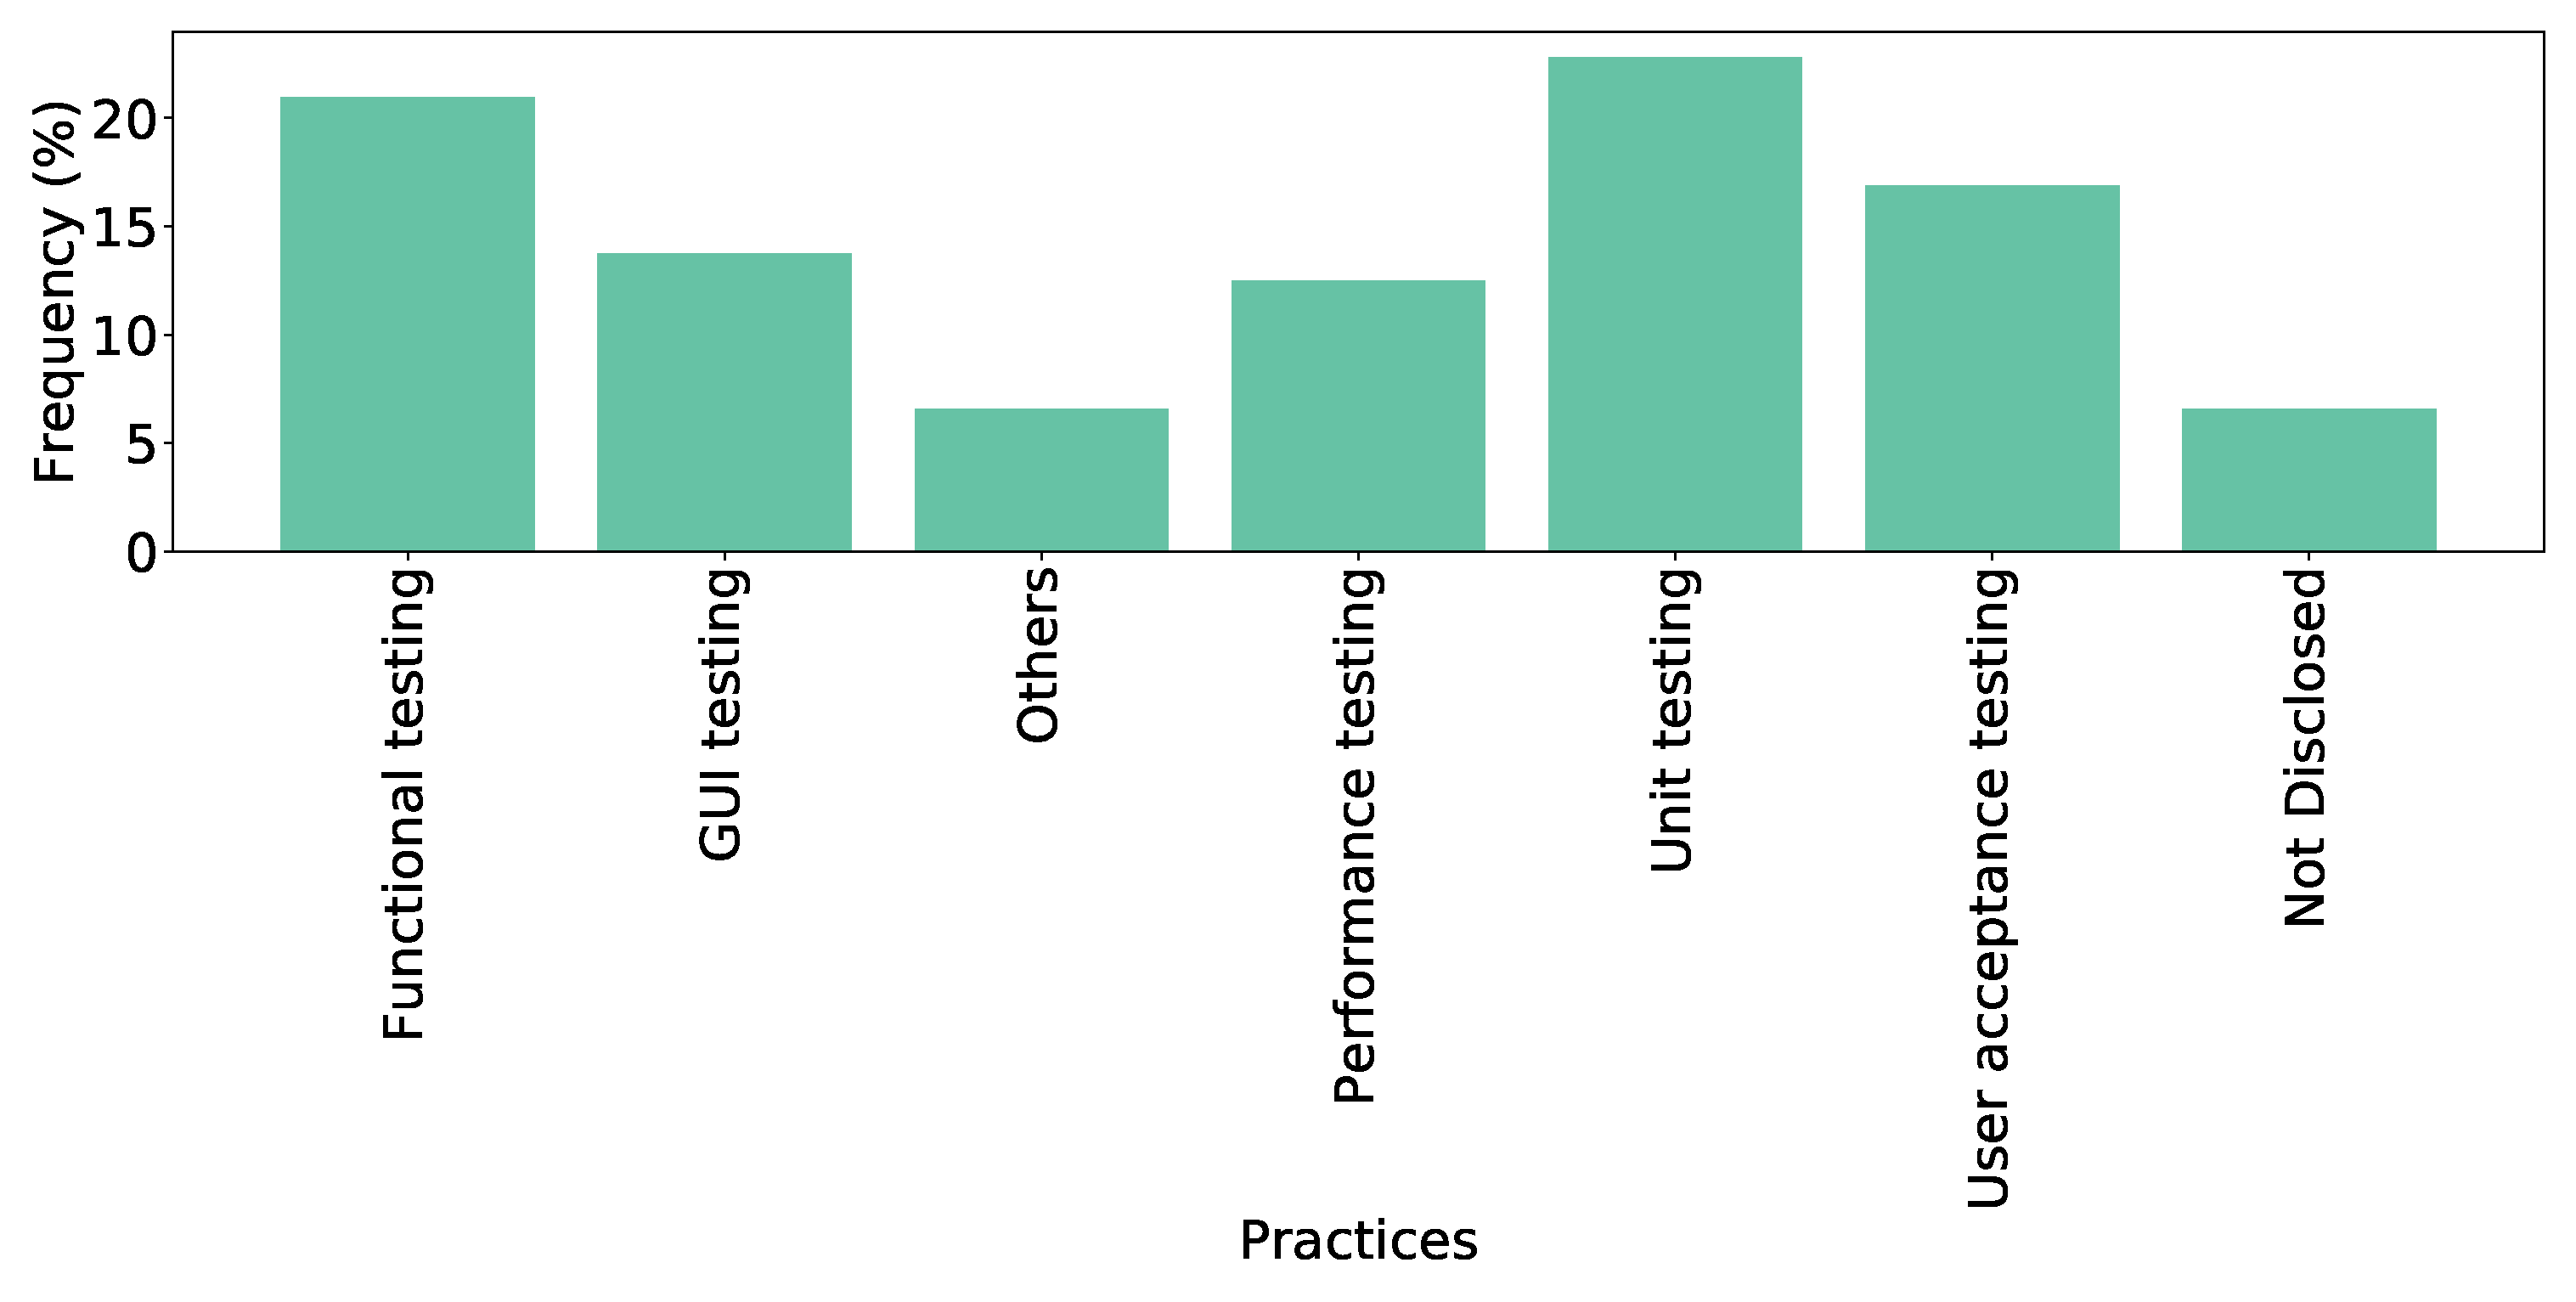
\includegraphics[scale=0.2]{Figures/Respondents_testing_practices}
  \caption{Testing Practices}
  \label{fig:testing}
\end{figure}


\paragraph{Level of Automated Testing}
Question 15 asked about the level of automated testing  performed in the company. The responses were gathered using the Likert scale. It was found that different respondents have very different experience in this context, i.e., some companies heavily practice automated testing, while others favor manual testing.  Results are shown in Figure \ref{fig:autoTest} which indicates that about 70\% of our respondents (others than who voted for level 5) do not use automated testing regularly. The level of automated testing might be related to the programming language/framework. The testing suite provided by framework/language might encourage developers to implement automated testing. The level of automated testing vs language and framework is plotted in Figures \ref{fig:language and autotest} and \ref{fig:framework and autotest}, respectively. It seems from Figure \ref{fig:language and autotest} that the highest level of automated testing is mostly practiced in Java, Javascript, Objective-C, and Php language. We conducted the Mann Whitney U test to assess our conjecture and it is found statistically significant ($p=0.01$). From Figure \ref{fig:framework and autotest}, we found that the highest level of automated testing is mostly performed in Android, Express, NodeJS, Struts, and Java EE framework, and the observation is statistically significant ($p=0.006$). Also, the highest level of automated testing is mainly used by developers (mostly use unit testing), and managers practice the lowest level of automated testing. The reason why managers use the lowest level of automated testing may be related to the type of testing they perform. We observed that managers mainly engaged in assessing the acceptability of the product from the end-user point of view. \anindya{Performance test may be automated. Thing about the previous comment. We may rather say that managers are likely to assess the acceptability from end user point of view.}\partha{updated} We guess that experience might be one of the factors that influence automated testing. Our conjecture was that senior developers might tend to use more automated tests than junior developers. We plotted experience and automated test levels in Figure \ref{fig:experience and autotest}. However, we found the opposite scenario, i.e., junior developers tend to use more automated testing than senior developers. However, the observation is not statistically significant ($p=0.08$). One of the reasons behind this observation may be that the senior developers perform certain testings (e.g., GUI testing), which are hard to automate.

\begin{figure}[h]
\centering
  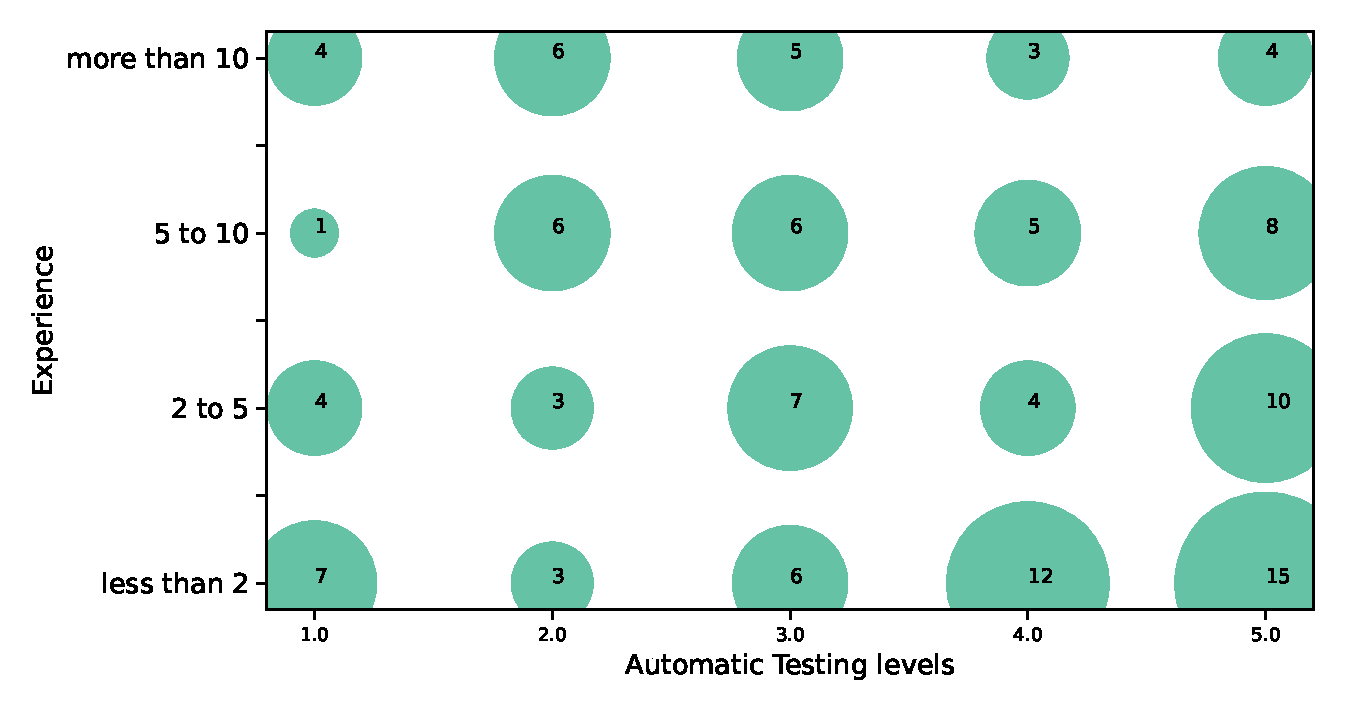
\includegraphics[scale=0.45]{Figures/Auto_Test_and_Experience}
  \caption{Experience and automated testing level}
  \label{fig:experience and autotest}
\end{figure}
\begin{figure}[h]
\centering
  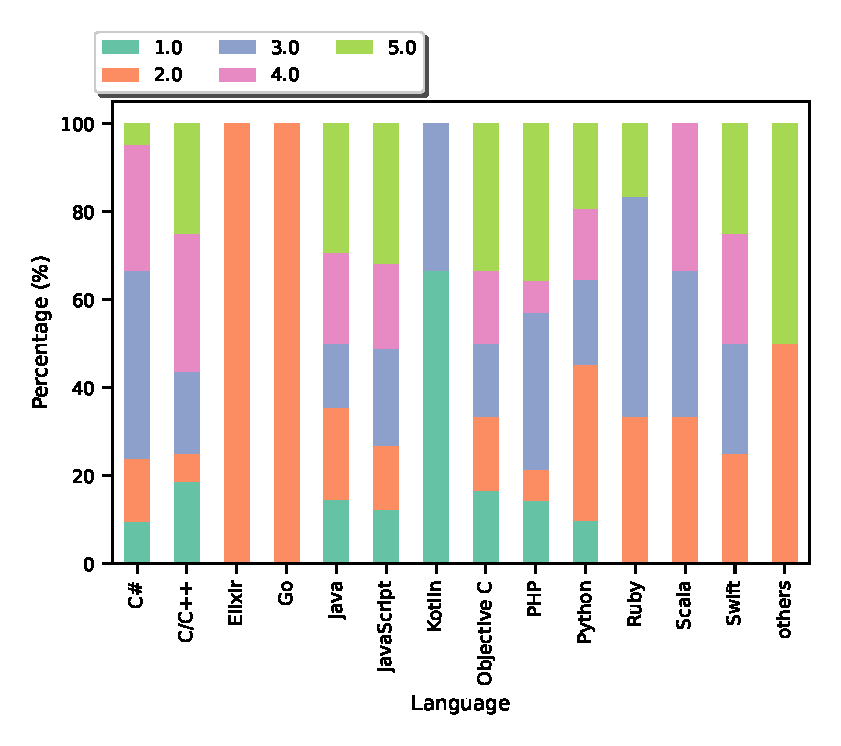
\includegraphics[scale=0.65]{Figures/Language_and_Test_Level}
  \caption{Programming language and automated testing level}
  \label{fig:language and autotest}
\end{figure}
\begin{figure}[h]
\centering
  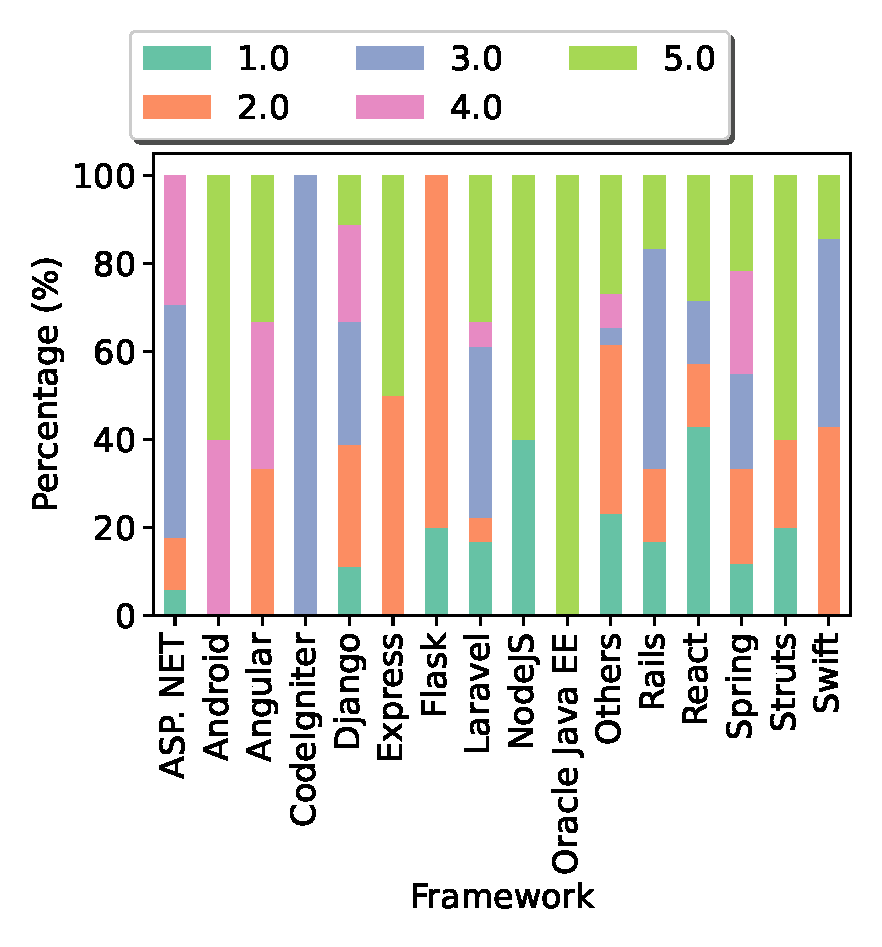
\includegraphics[scale=0.65]{Figures/Framework_and_Test_Level}
  \caption{Framework and automated testing level}
  \label{fig:framework and autotest}
\end{figure}

\begin{figure}[h]
\centering
  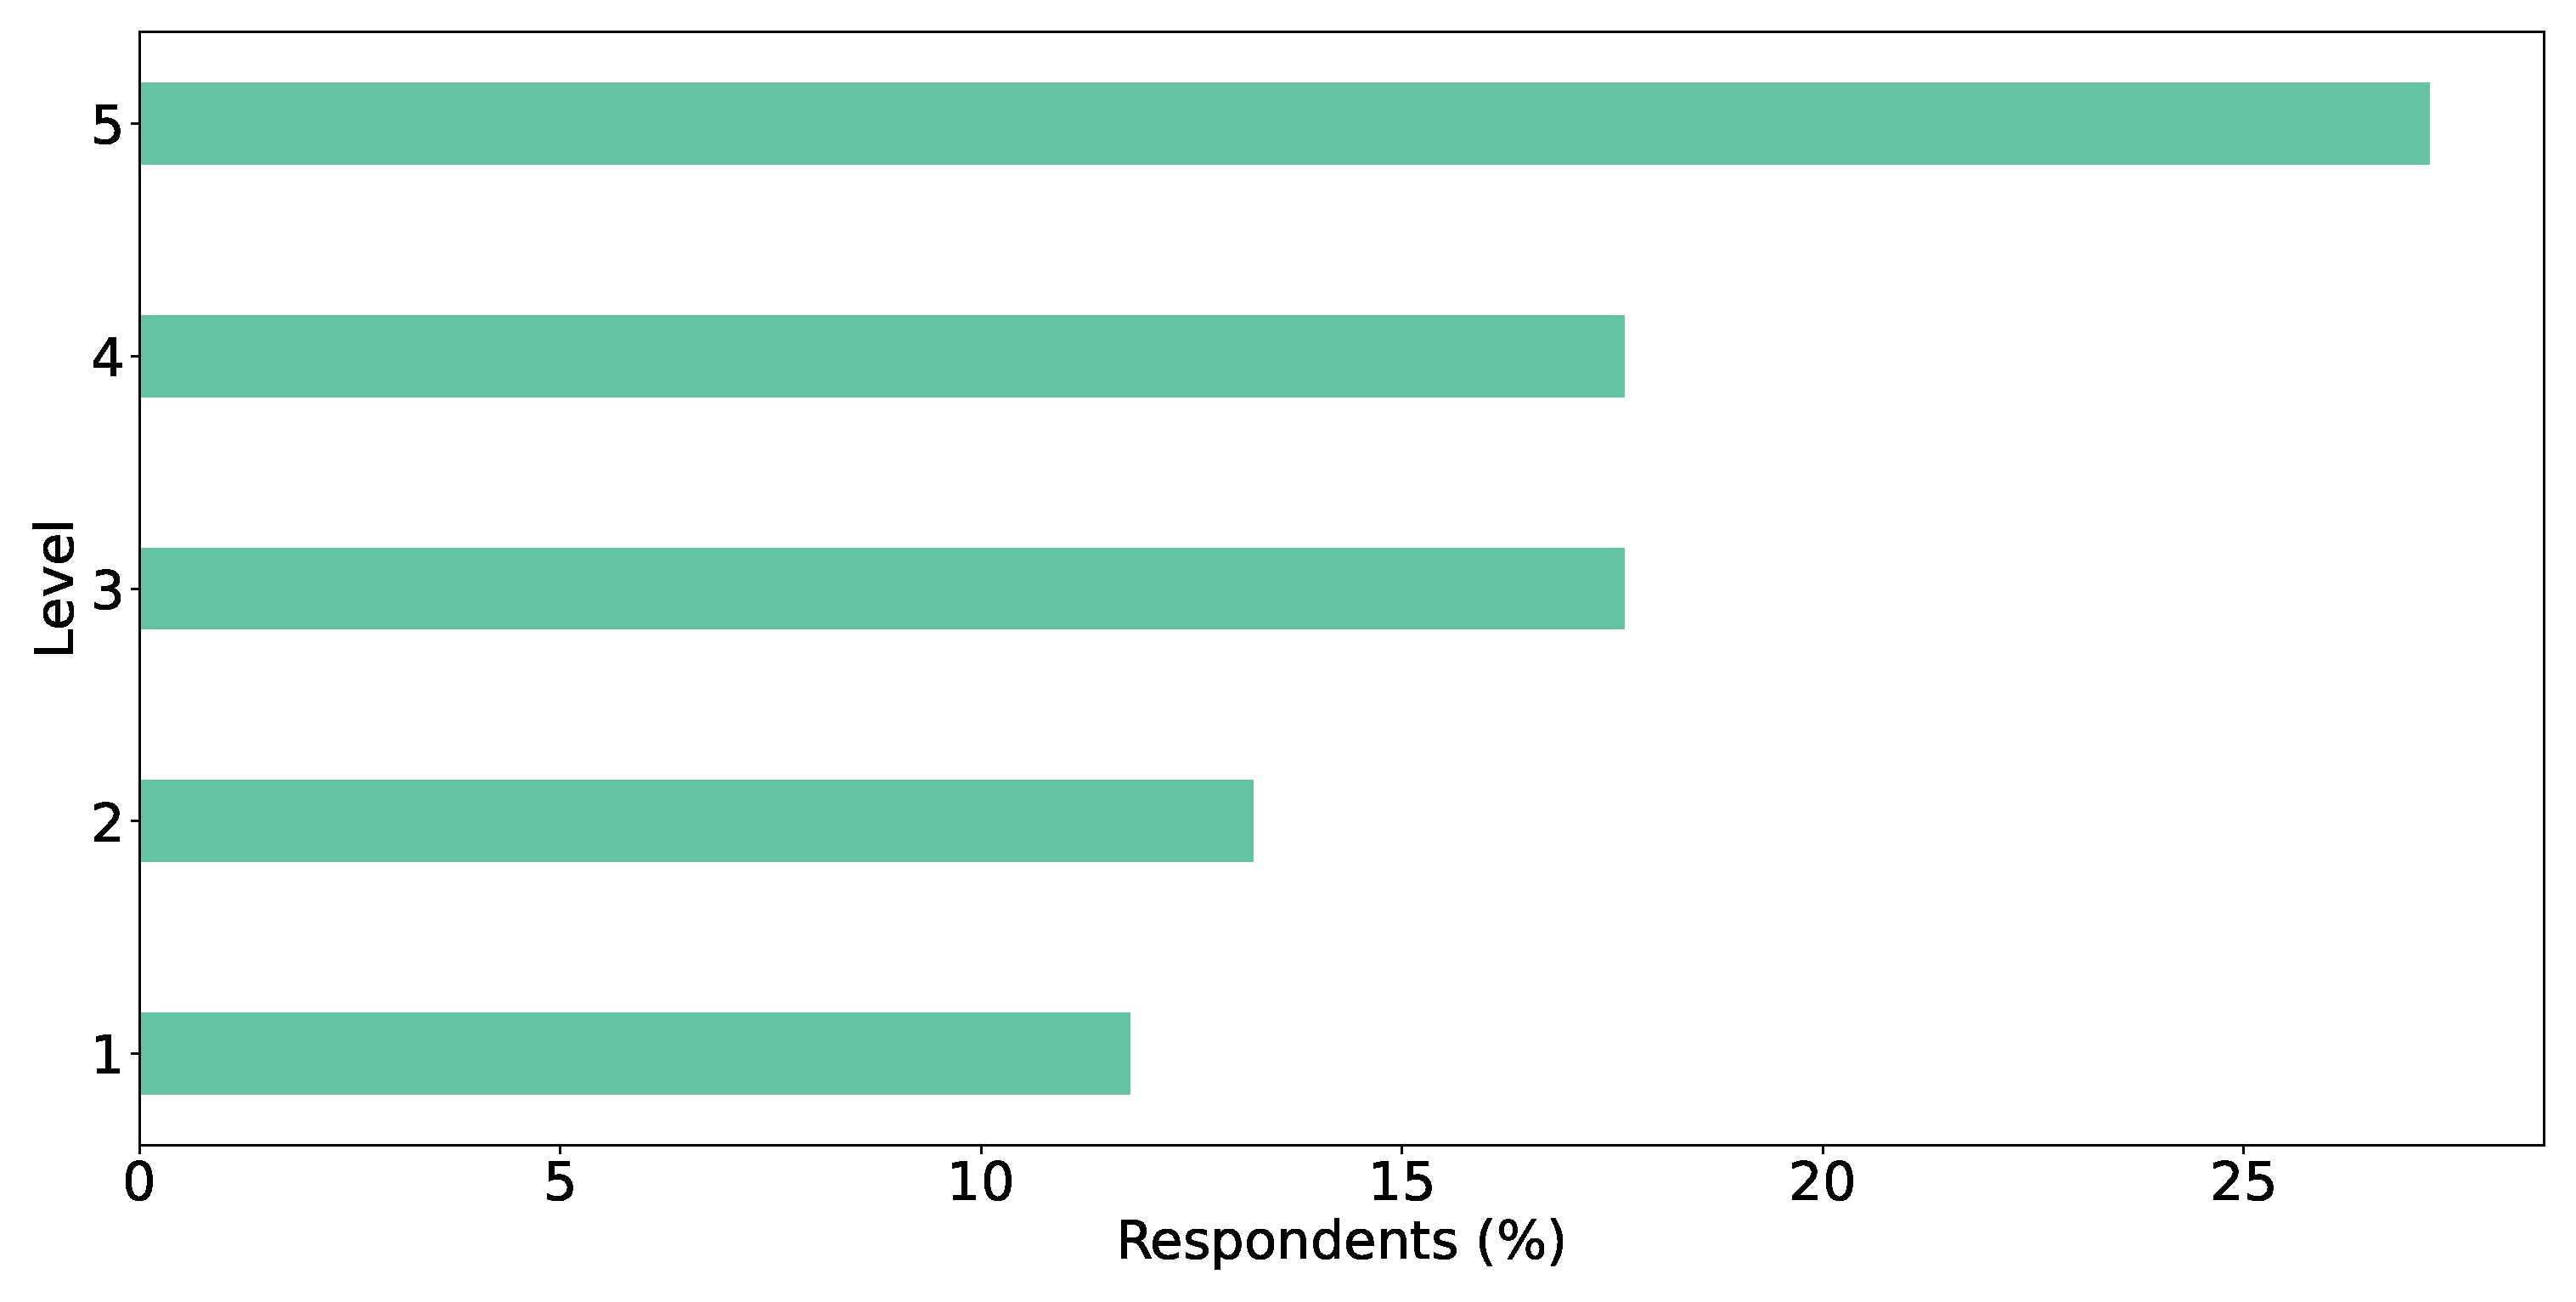
\includegraphics[scale=0.15]{Figures/Respondents_autotest_level}
  \caption{Automated Testing Level}
  \label{fig:autoTest}
\end{figure}

\boxtext{There exists a tendency among most of the Bangladeshi developers not to use automated testing regularly.}
\anindya{Can it be the case that automated testing is done by SQA team, not regular developers?}


\paragraph{Tools Used in Testing and QA}
Q16 asked about the tools used in testing and quality assurance. According to \ref{fig:testingTools}, we see that most of the respondents have used XUnit( eg, JUnit, NUnit) (30\%), selenium (27\%), Jenkins (20\%), others (9\%). These results show that there exists a great demand for testing tools in the software industry of Bangladesh. However, around 38\% of our respondents were not interested to reply to this question that is not surprising because the majority of the respondents (93\% approx.) were working on roles other than SQA engineer as per Table \ref{tab:role}, and they are not supposed to be involved in any testing themselves. \anindya{This may be because many developers are not involved in any sort of testing themselves and our respondents are dominated by developers.} \khalid{added}

\begin{figure}[h]
\centering
  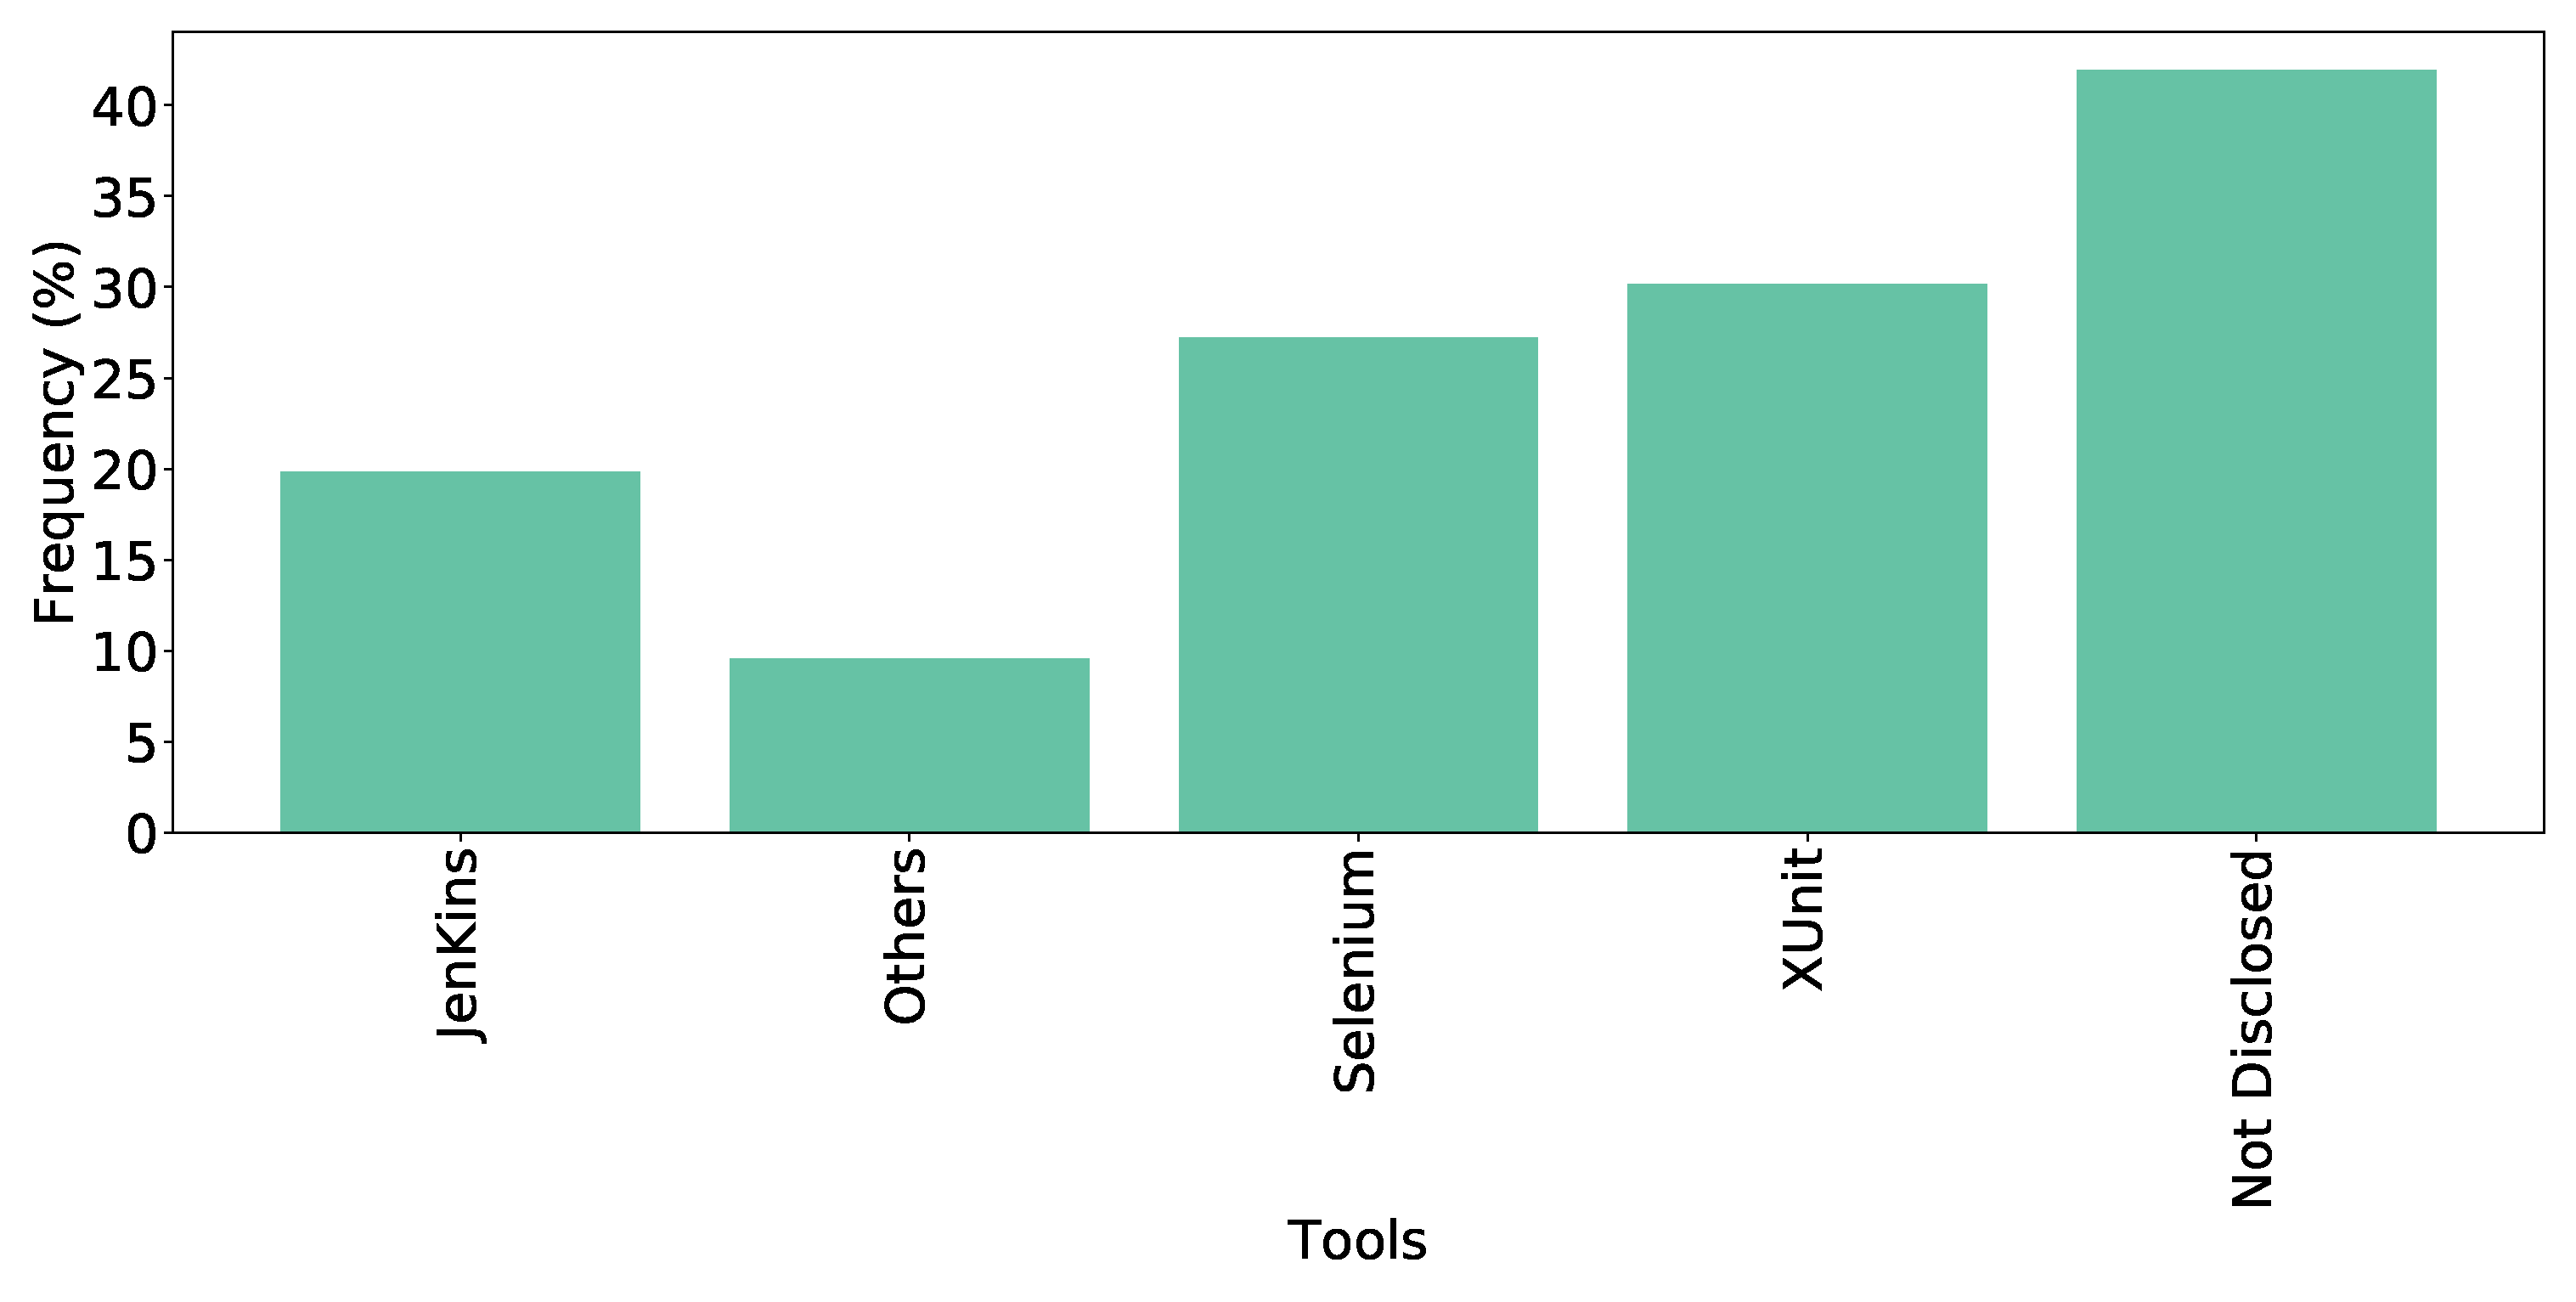
\includegraphics[scale=0.18]{Figures/Respondents_testing_tools}
  \caption{Testing \& QA Tools}
  \label{fig:testingTools}
\end{figure}

\boxtext{There has a large demand of software testing tools in Bangladesh.}


\paragraph{Deployment Tools}
According to \ref{fig:deployTools}, we see that most of the respondents deploy their implemented codes using AWS code-deploy (12\%) and Jenkins (12\%). The other deployment tools are Bamboo (5\%), TeamCity (4\%), Octopus (2\%), etc. Respondents voted none (4\%) as they didn't use any deployment tools and 53\% of the respondents were not interested in this topic. Anyhow, the percentage of the uninterested respondents does not seem unexpected. From Table \ref{tab:role} and \ref{tab:experience}, we can observe that a significant portion of our respondents is developers, and more than half of our respondents are experienced for less than five years respectively. As deployment is related to DevOps, it is quite likely that developers have not enough knowledge or have less interest in deployment. \anindya{Again, this is mostly a dev op related issue and the developers are not likely to respond in this regard.} \khalid{added} The outcome indicates that the usage rate of deployment tools in Bangladesh for continuous integration and continuous deployment is yet to be widespread. We also guessed that the practice of using deployment tools might be done only by senior practitioners. However, the hypothesis is not statistically significant ($p=0.37$).

\begin{figure}[h]
\centering
  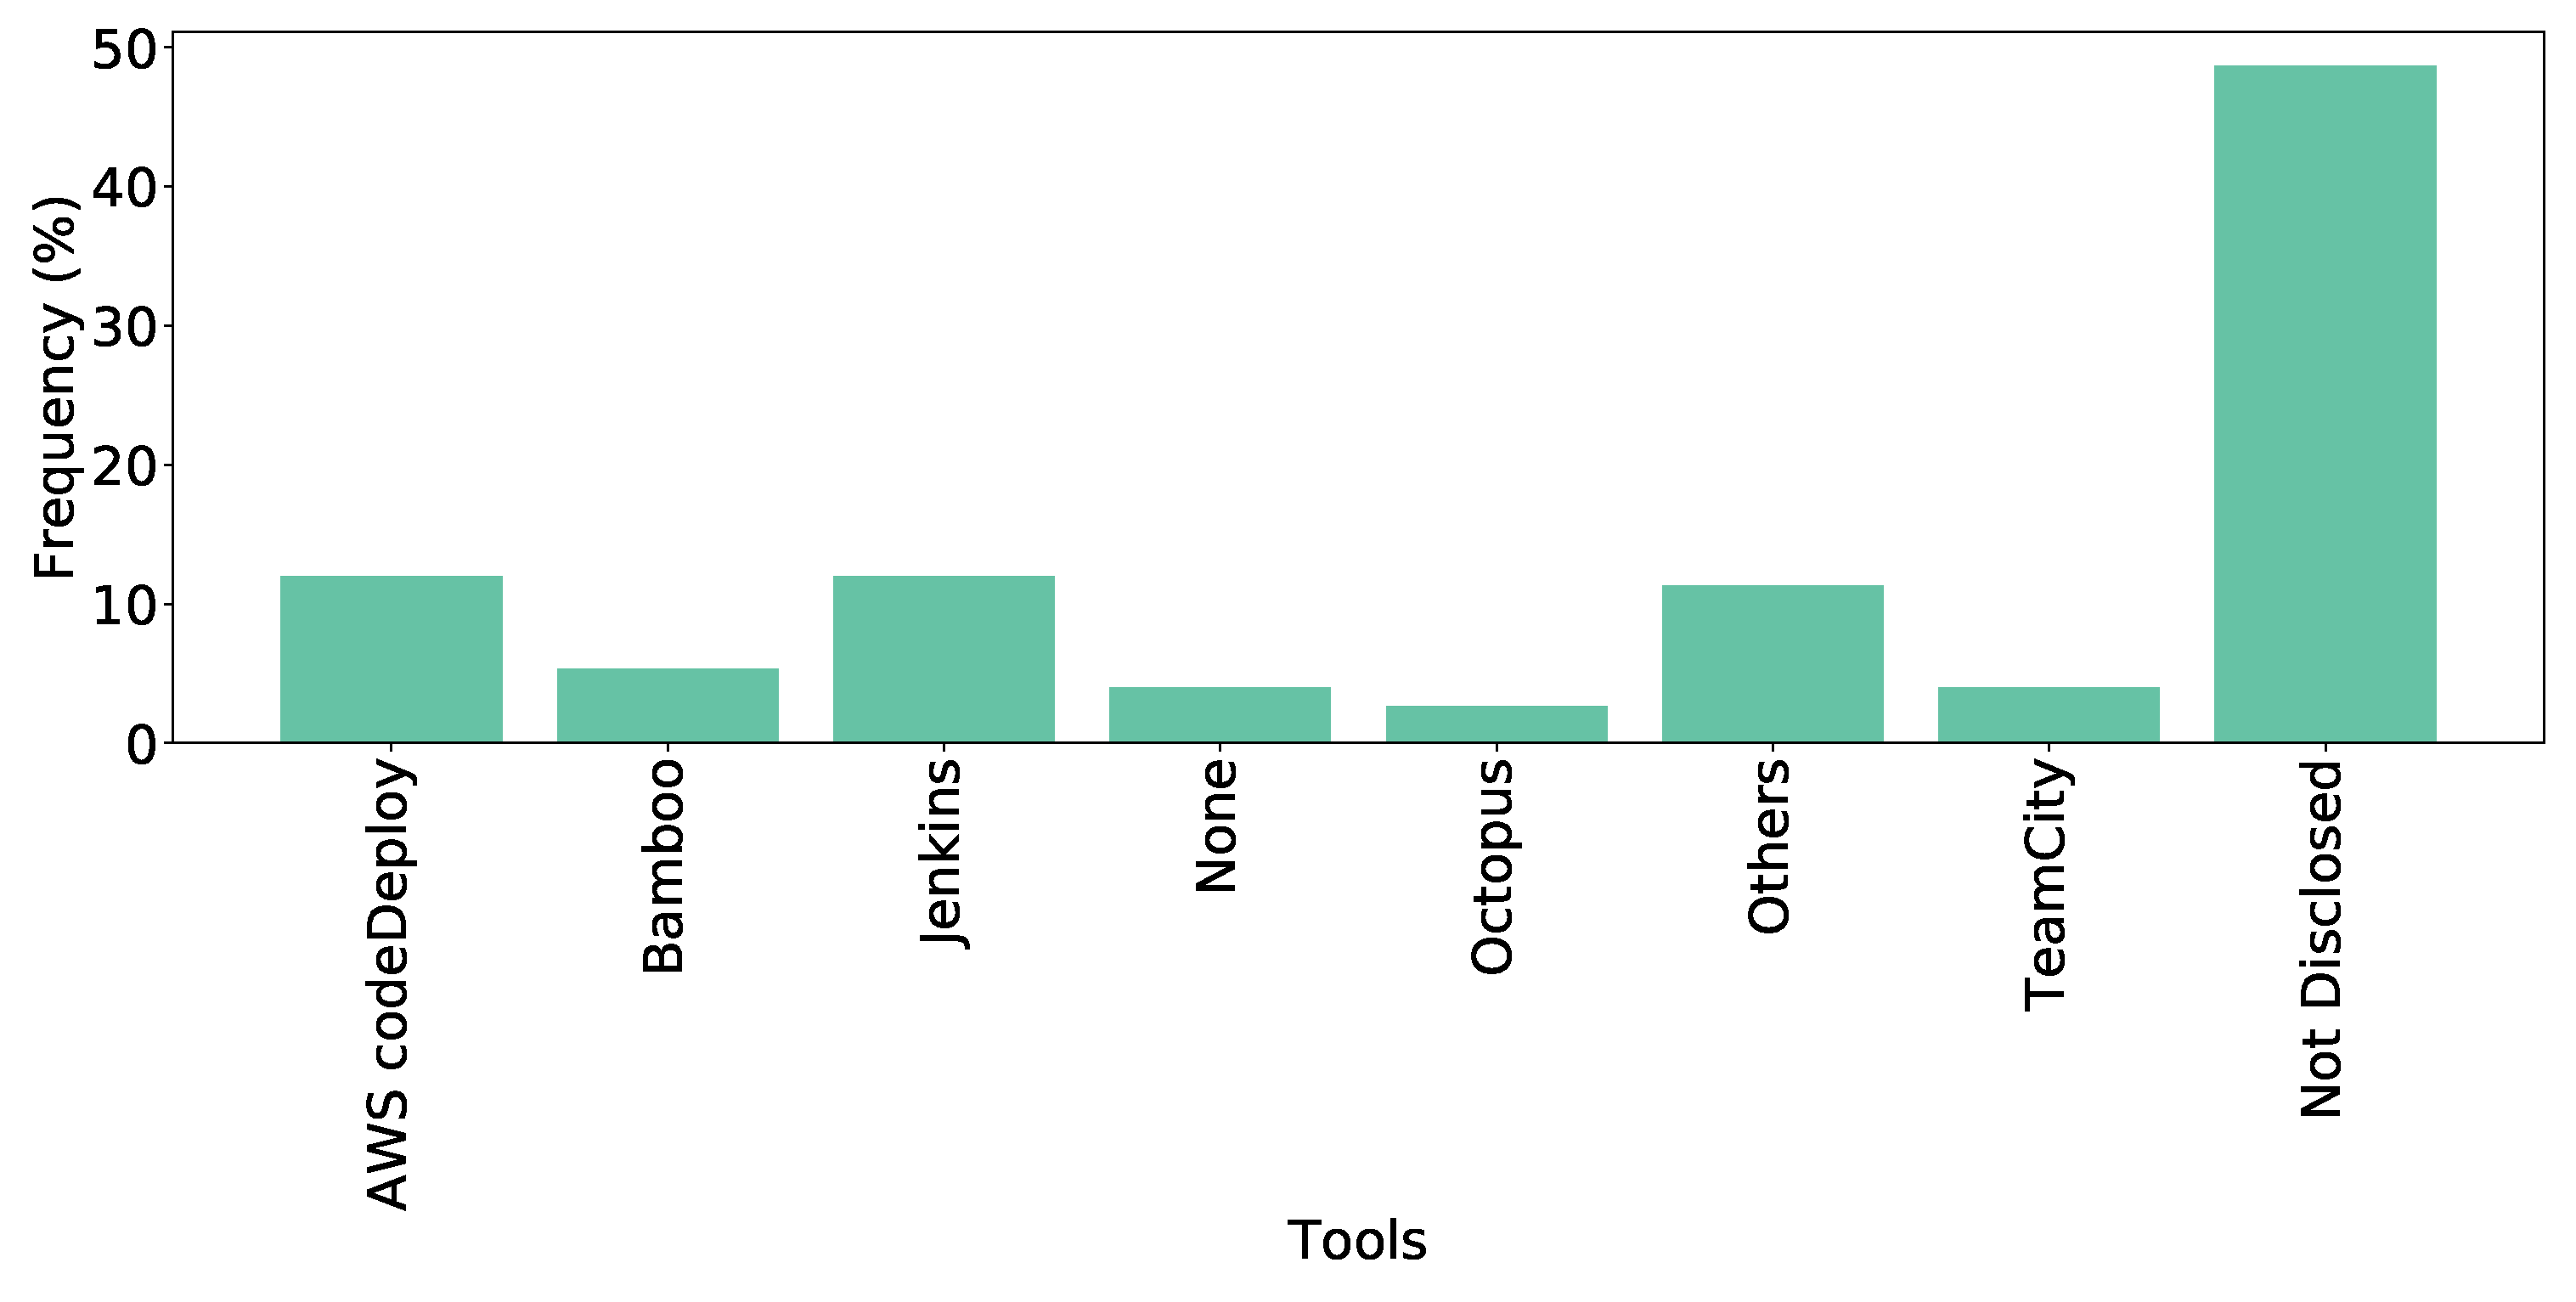
\includegraphics[scale=0.18]{Figures/Respondents_deployment_tools}
  \caption{Deployment Tools}
  \label{fig:deployTools}
\end{figure}


\paragraph{Version Control}
% \hfill\\

Respondents were allowed to select more than one option. As shown in Figure \ref{fig:versionControl}, Git (78\%) and Bit-Bucket (29\%) are mostly-used version control systems in the software industry. Besides these, Subversion (SVN) (5\%) and others (4\%) are used.  The 2018 Stack overflow survey\cite{StackoverflowSurvey2018} reports that the most popular version control system is Git (87.2\% developer uses Git) and the second most popular is SVN (16.1\% developer uses SVN). However, in our survey, we found a slightly different result, the most popular version control system is Git and the second most popular is Bit-bucket. This might be related to the declining popularity of SVN over the years. From the Stack overflow survey over the range 2017-2018, it is clear that SVN is losing popularity to Git. Nowadays, SVN is mainly used for versioning legacy projects. As the SE industry of Bangladesh is relatively young, this discrepancy observed is not surprising.
\anindya{It looks nice that you compared with external relevant source like SO. Is it possible to do it for other RQs? Also, you may mention such deviations from other trends in Introduction.} \khalid{added in `methodologies', `tech platform', `test practices'} \partha{added in `os', `languages', `framework'}
\begin{figure}[h]
\centering
  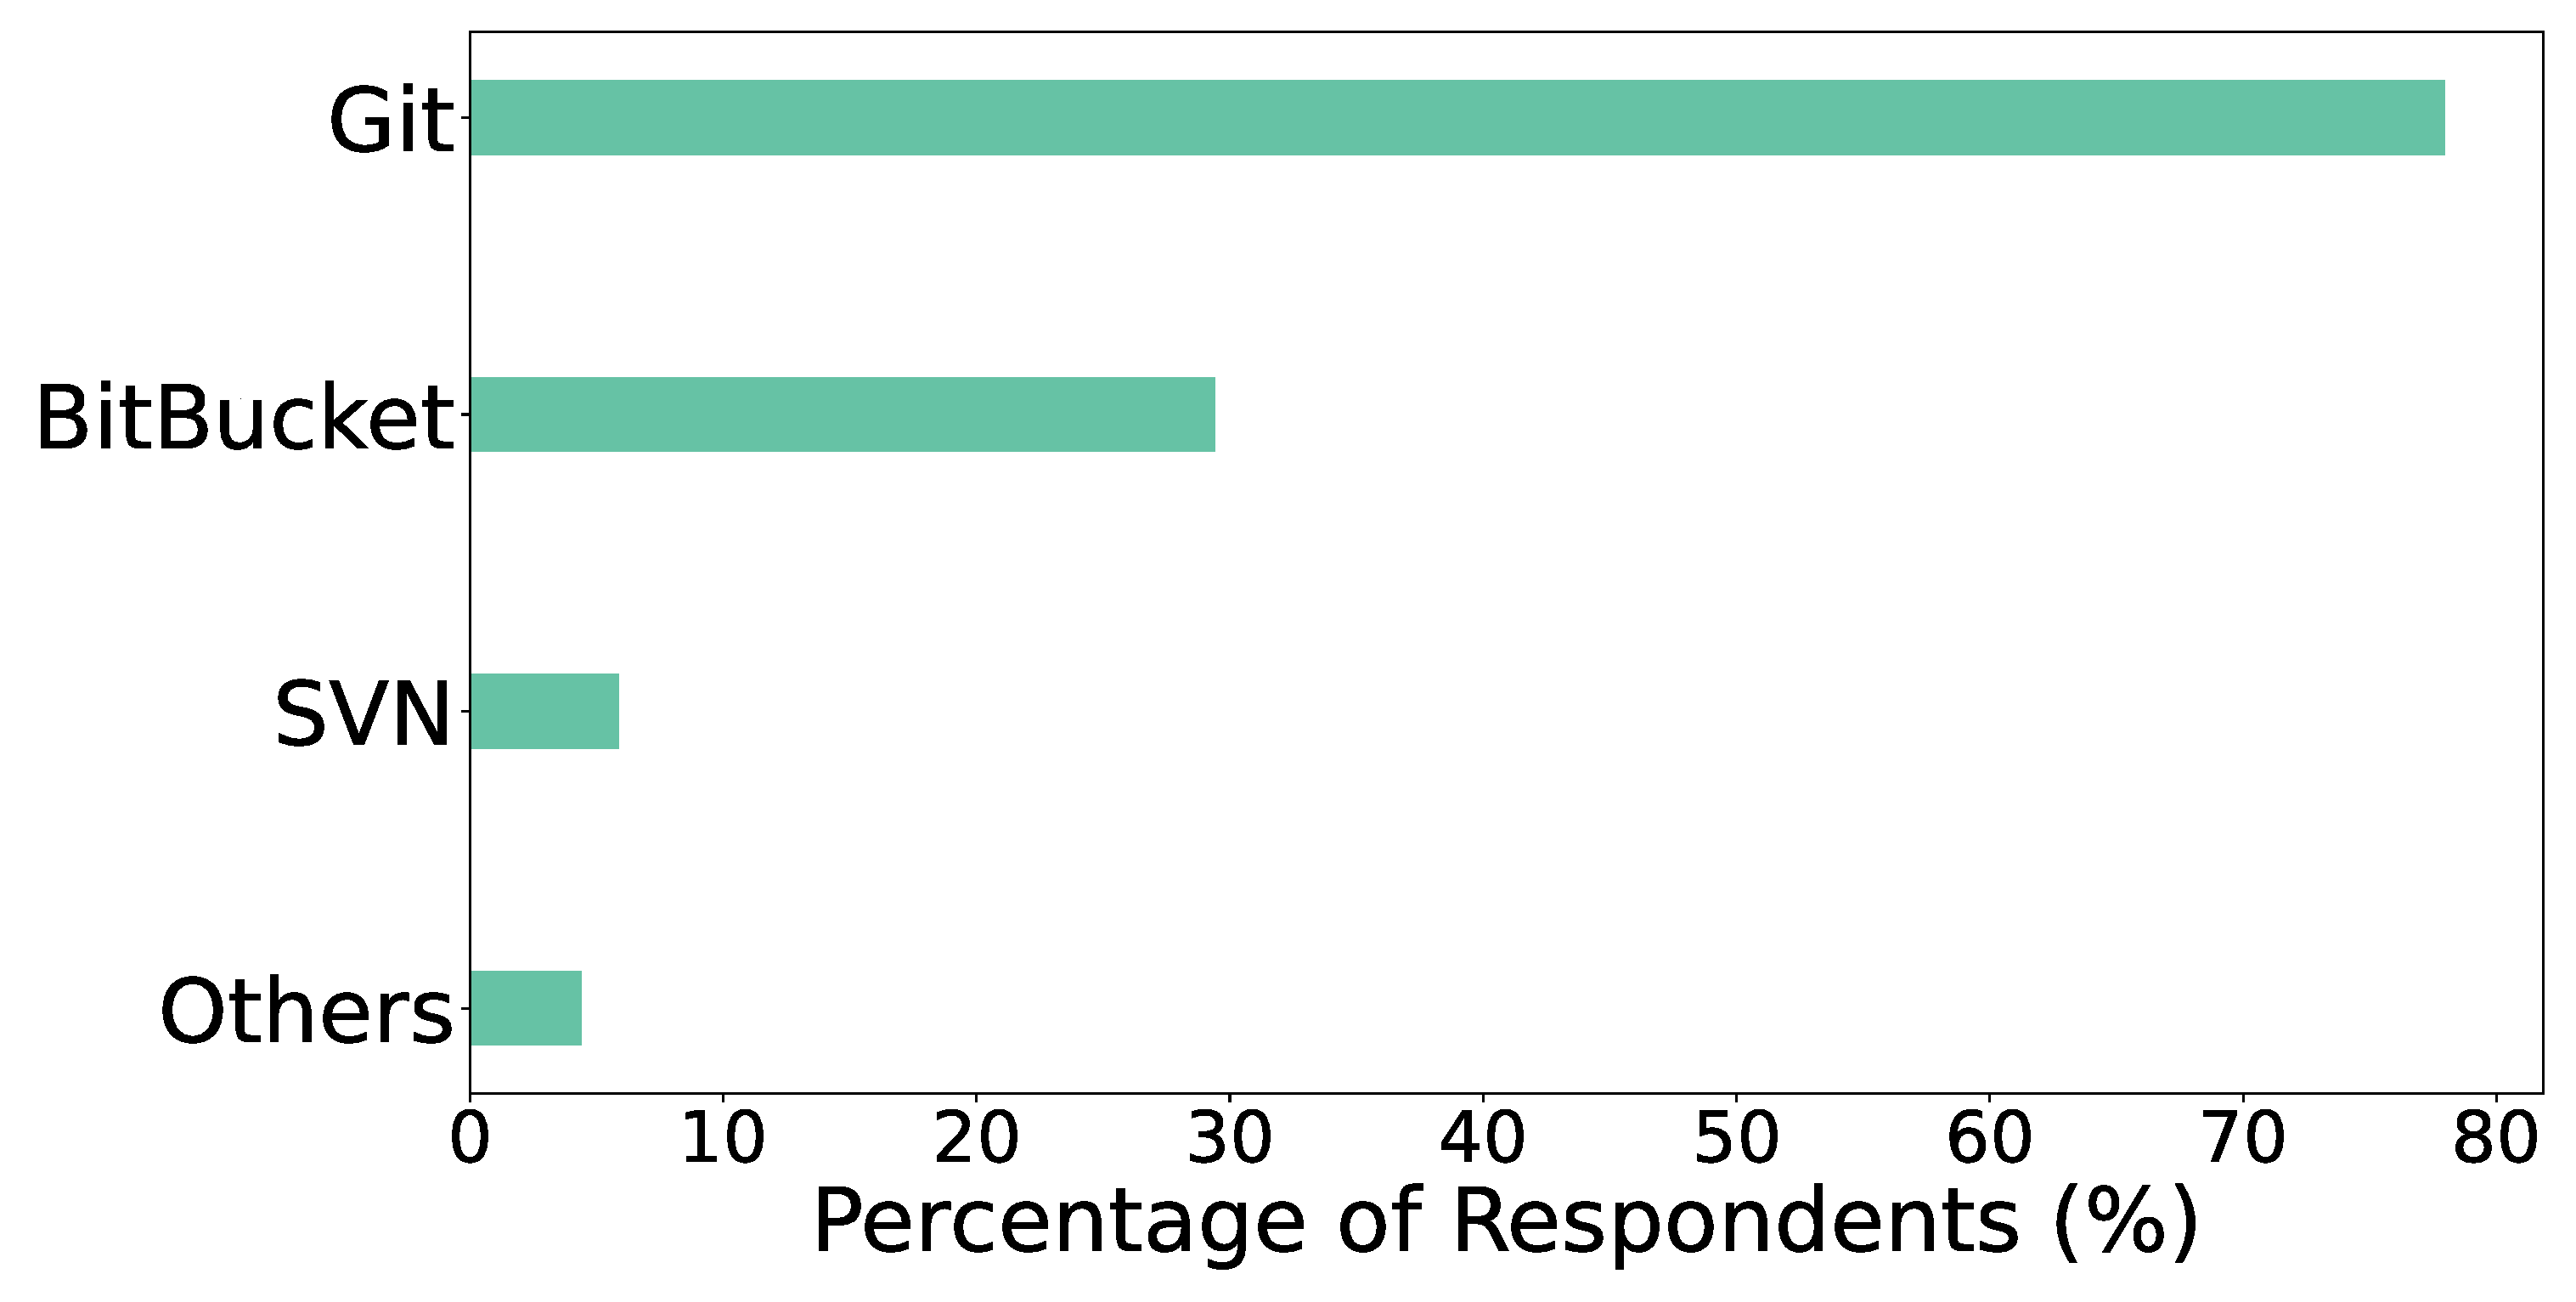
\includegraphics[scale=0.16]{Figures/Respondents_version_control}
  \caption{Version Control}
  \label{fig:versionControl}
\end{figure}

\subsubsection{Performance and security measures used (D4)}
\label{security_performance}
Security and performance are two of the most important non-functional requirements for any software product. 
We asked three open-ended questions with regards to the enforcement of security and performance-related features in software products in Bangladesh:
How do you ensure performance, scalability (Q21, Q22) and security (Q23) in your software products?

% To identify general practices among the Bangladeshi software companies regarding software products' security and performance, we have included two open-ended questions in the survey. This particular question covers how a company secures its developed products from security threats and maintain performance after deployment. However, the scalability of software directly impacts its performance\citep{Liu2009,Bondi2000}. Hence, we will cover the following points here:
% \begin{itemize}
%     \item Security
%     \item Performance
%     \item Scalability
% \end{itemize}


%\label{Security}

\begin{figure}[h]
\centering
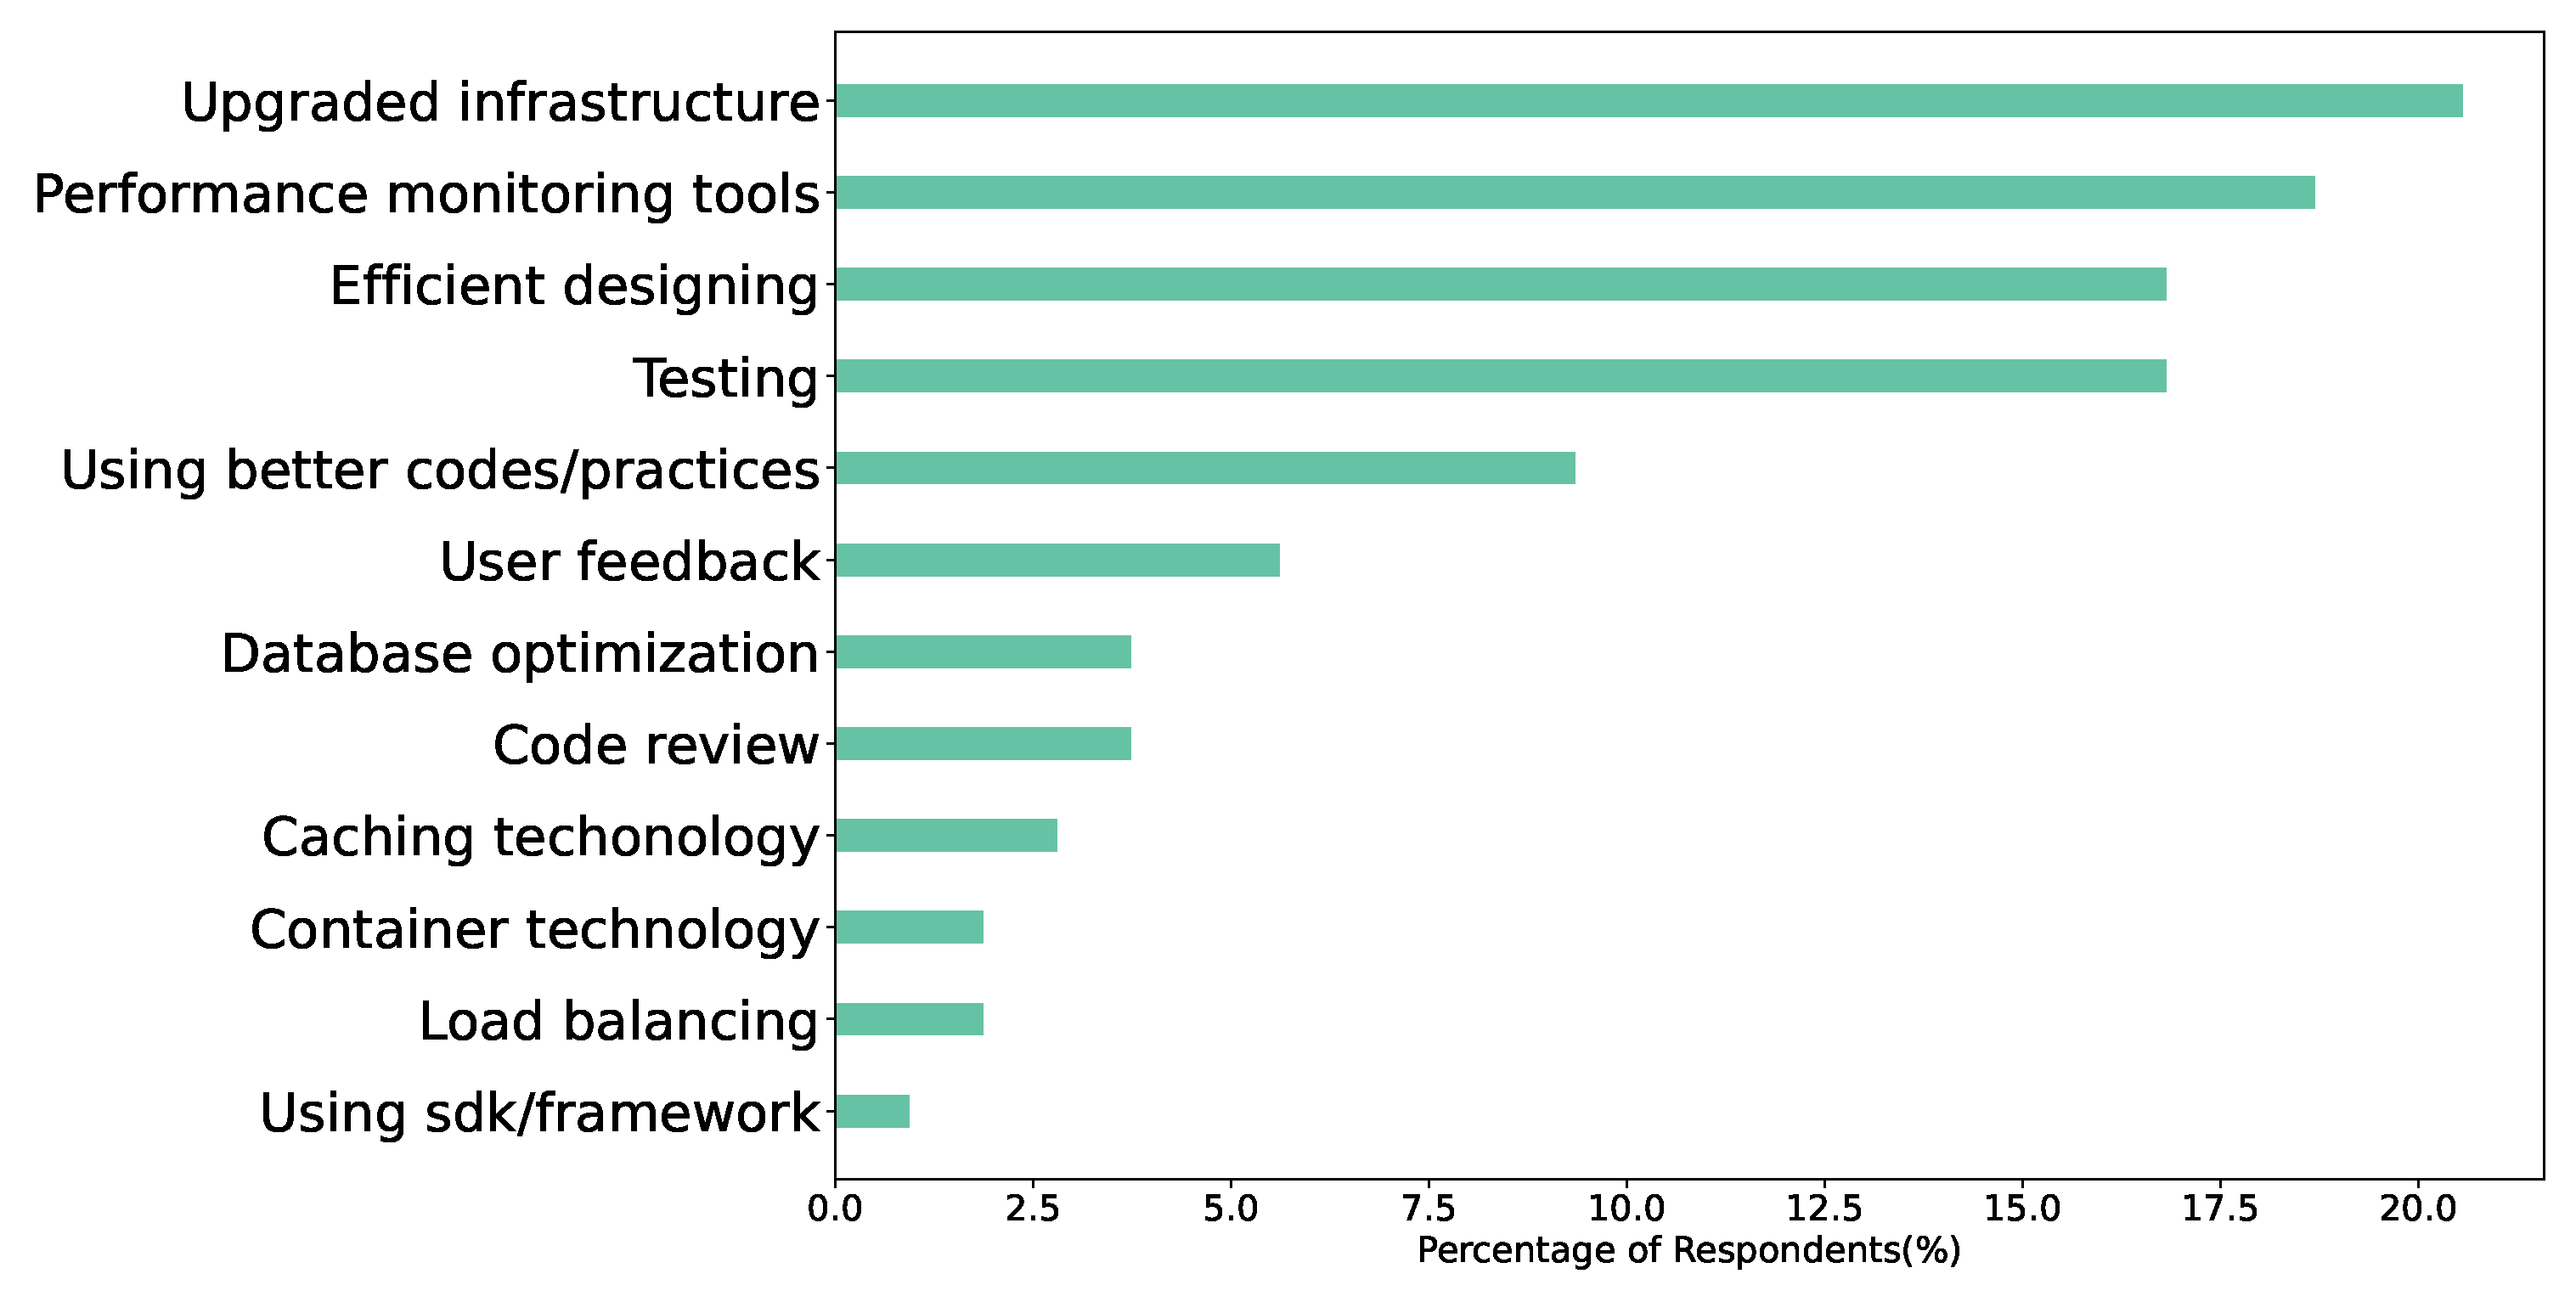
\includegraphics[scale=0.22]{Figures/PerformanceScalability.eps} 
\caption{Measures to ensure performance \& scalability of products}
\label{fig:Measures to ensure performance and scalability}
\end{figure}
\nd\bf{$\bullet$ Performance (Q21, Q22).} Software performance indicates how efficient the software is in terms of response time and resource consumption. 
We find nine types of performance measures that are practised in software products developed in Bangladesh (see Figure \ref{fig:Measures to ensure performance and scalability}).  
The twelve types are divided into four categories: 
\begin{inparaenum}
Use of \item tools and frameworks (46.72\%),
\item design principles/best practices (26.17\%),
\item testing (16.82\%), and
\item review and feedback (9.35\%).
\item database optimization (3.74\%)
\end{inparaenum} 

\begin{inparaenum}[(1)]
\item \ib{Exploitation of tools and frameworks.} Six out of twelve types belong to this category.
\begin{inparaenum}%[label=(\alph*)]
    \item \it{Tools}: Around 18.69\% respondents use tools and metrics to
    measure performance:  \emt{take help of different performance monitoring tools and dashboard, analyzed data, measure time and memory efficiency of process}($S_{35}$)
    \item \it{Infrastructure}: Around 20.56\% of respondents use upgraded
    infrastructure to ensure performance like cloud
    hosting (e.g., Amazon AWS), a high-end server, and new technologies.
    %\emt{Amazon Hosting and Quality Software}{85}
    \item \it{Caching}: Around 2.8\% respondents implemented caching to maintain
    software performance.
    % \emt{... Good Caching}{29}
    \item \it{Container Technology}: Containers enable users to scale their system without any dependency on the underlying OS. About 1.87\% of our respondents use container technologies to ensure their products scalability and performance.
    \item \it{Using SDK/framework}: About 0.93\% of respondents depend on the framework to maintain software performance and scalability.
    \item \it{Load Balancing}: Around 1.87\% respondents use load
    balancing as a measure to maintain performance:
    \emt{Optimizing number of HTTP requests, Asynchronous programming, Caching, CDN, Load Balancing, nginx, varnish, compression of data, 
    Continuous monitoring, Load testing, stress testing}($S_{42}$)
\end{inparaenum}
 
\item \ib{Use of design principles/best practices.}  Around 26.17\% respondents try to ensure software performance right from the design phase as follows.
\begin{inparaenum}%[label=(\alph*)]
    \item \it{Using better codes/practices}: Around 9.35\% respondents ensure performance by
    implementing industry-standard best practices like compression
    technology, enforcing design patterns, and refactoring.
    %\emt{Implementation time carefulness and maintaining a well developed coding standard}{40}
    \item \it{Efficient designing}: Around 16.82\% of respondents emphasize on
    performance-aware architecture design.
    %\emt{By careful designing}{24}
\end{inparaenum}

\item \ib{Use of testing.} Around 16.82\% respondents rely on the software testing strategy to ensure performance like load testing and stress testing.

\item \ib{Use of review and feedback.} Around 9.35\% of our respondents use user feedback (e.g., continuous feedback from QA team $S_{65}$) 
and code review to improve product performance. According to $S_{15}$: \emt{The code quality is assessed by the different team members during code review, followed by designing new ways to solve issues in the product that are time-intensive.}

\item \ib{Database Optimization.} Around 3.74\% of our respondents use database optimization to ensure performance and scalability. Database optimization includes sharding, clustering, indexing, and scaling. According to $S_{85}$: \emt{Besides scaling horizontally, database scaling is performed by partitioning tables, along with multi-threaded implementations}

\end{inparaenum}


\begin{figure}[h]
\centering
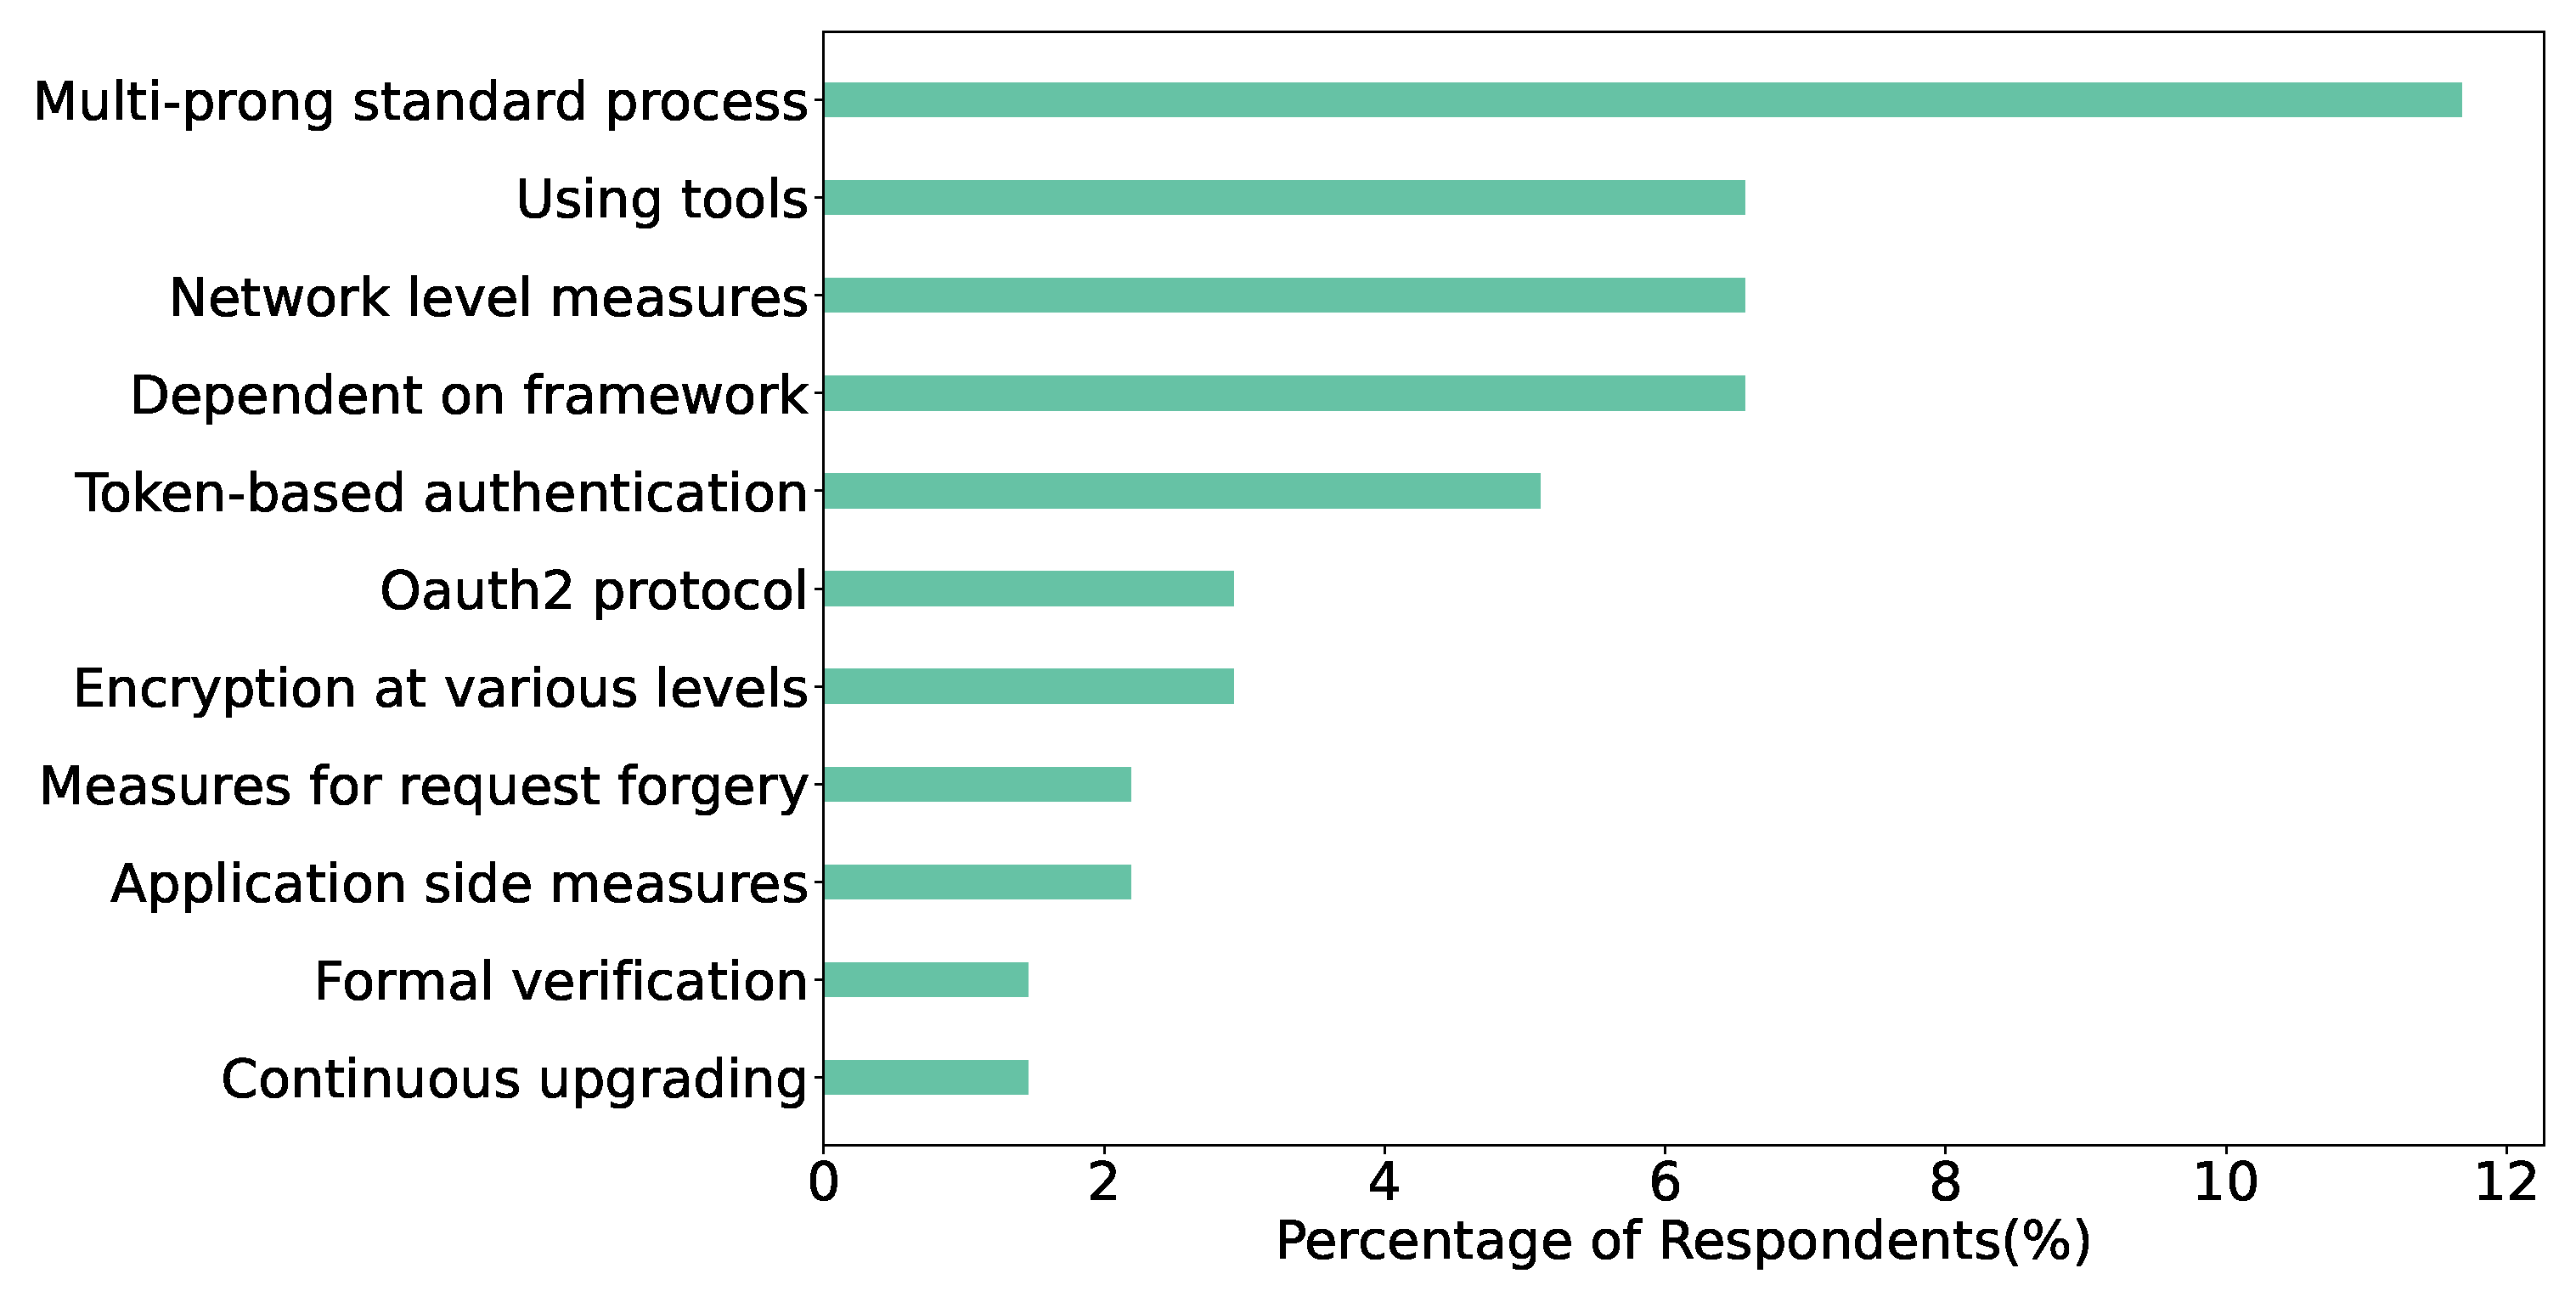
\includegraphics[scale=0.22]{Figures/Security.eps} 
\caption{Measures to ensure security of products}
\label{fig:Measures to ensure security}
\end{figure}
\nd\bf{$\bullet$ Security (Q23):} Our open coding of the survey responses reveals 11  
labels (see Figure \ref{fig:Measures to ensure security}). The 11 labels are are divided into three main categories of security-related development practices: 
\begin{inparaenum}
\item Measures related to authentication and authorization (64.82\%),
\item Exploitation of tools and techniques to ensure security in products (53.71\%), and 
\item Use of encryption technologies for data (7.41\%).
\end{inparaenum} We discuss the categories below.  


\begin{inparaenum}[(1)]
\item \ib{Measures related to authentication and authorization.} Six out of the 11 labels belong to this category. 
\begin{inparaenum}
\item \it{Multi-prong Standard Process}. About 29.6\% of the respondents
reported that they practice various security standards and protocol to
ensure security (e.g., ISO/IEC 27001, PA DSS).
\item \it{Token-based authentication.} About 13\% respondents reported to 
have implemented a token-based authentication system, which 
allows users to enter their username and password to obtain a token for authentication and authorization.
\item \it{OAuth 2.0} : Around 7.4\%) respondents use the OAuth 2.0
protocol as the primary way of maintaining security. OAuth 2.0 is the industry-standard protocol for
authorization. OAuth 2.0 focuses on client developer simplicity while providing
specific authorization flows for web applications, desktop applications, mobile
phones, and living room devices. %, e.g., \emt{OAuth 2.0,
\item \it{Application-side measures}: Around 5.6\% of respondents 
implement security measures at the application level like encryption of application data at the client-side, use of https while
pulling data from a server, secured architecture, etc.
\item \it{Measures for request forgery}: Around 5.6\% respondents implemented security measures against
Cross-site request forgery (e.g., attacks like
cross-origin resource sharing (CORS), cross-site request forgery (CSRF) or
one-click attack or XSRF). Security testing is paramount for this: \emt{Security testings
like: SQL injection, cross-site scripting, CSRF, API security, use of https, 
detecting malicious/suspicious HTTP requests and auto-blocking} (Respondent ID $S_{42}$)
    \item \it{Formal Verification}: Around 3.7\% respondents ensured the practice of formal code review to enforce security practices: \emt{There are some basic
    guidelines that we must follow and while code review this needs to be an
    absolute part that needs to be checked before the code gets merged} ($S_{112}$)
    \end{inparaenum}

\item \ib{Exploitation of tools and techniques to ensure security in products.} Four out of the 11 labels belong to this category. 
\begin{inparaenum}
  \item \it{Dependent on Framework}: Around 16.7\% 
  respondents depend on the underlying framework for security like Spring, HDIV, and Laravel. 
  \emt{https, popular framework which already prevents some type of attacks. rest of the things on case-by-case basis)}($S_{79}$)
  \item \it{Use of tools}: Respondents use various open-source/paid tools for
  scanning and testing like OWASP and penetration testing tools.
  %\emt{use encryption at different level of software (server, network, transmission layer, database and software layer.)}{35}
  \item \it{Network level Measures}: Network-level measures include
  IP-white-listing, port-blocking, VPN, and the use of HTTPS in software.
  16.7\% of respondents use at least one of the mentioned strategies to ensure
  security.
  %\emt{network blocking and common security measures}{2}
  \item \it{Continuous Upgrade}: Around 1.5\% 
  respondents reported that they arrange frequent hackathons, workshops, and
  security audits: \emt{We run security audit of our office environment. We also conduct security session per 6 months to introduce latest trend in threats and what we can do to avoid it}($S_{57}$)
\end{inparaenum}

\item \ib{Use of encryption technologies for data}. Around 7.4\% respondents use encryption at
the different levels of software architecture such as network, data, and
transmission.
\emt{use encryption at different level of software (server, network, transmission layer, database and software layer.)}($S_{35}$)
\end{inparaenum}
% 
% Authentication and authorization based security are the most prominent practices in the software industry of Bangladesh. The other techniques used widely include framework, platform, tools, and encryption. Under these categories, several measures are usually followed. The security measures of the Bangladesh SE industry is presented in Figure \ref{fig:Measures to ensure security}. The measures of each category are discussed below.
% 
% Measures under the \emph{authentication and authorization} category is practised by 53.71\% respondents to ensure security. The measures are 
% \begin{enumerate}[label=(\alph*)]
% 
%     \item \textbf{Multi-prong Standard Process}: About 29.63\% of the respondents reported that they practice various security standards and protocol to ensure security. The standard includes ISO/IEC 27001 and PA DSS.
%     \surveyquote{Multi Prong Standard Processes and Products}{110}
%     
%     \item \textbf{Token-based authentication}: A token-based authentication system allows users to enter their username and password to obtain a token, which allows them to fetch a specific resource without using their username and password. Once their token has been obtained, the user can offer the token, which offers access to a specific resource for a time period to the remote site. 12.96\% of people expressed its eligibility.
%     \surveyquote{Token based authentication for all of my rest service}{80}
%     
%     \item \textbf{OAuth 2.0} : OAuth 2.0 is the industry-standard protocol for authorization. OAuth 2.0 focuses on client developer simplicity while providing specific authorization flows for web applications, desktop applications, mobile phones, and living room devices. Many (7.41\%) respondents use the OAuth 2.0 protocol as the primary way of maintaining security.
%     \surveyquote{OAuth 2.0, JWT, Token Based Authentication, CORS Filter, XSRF}{127}
%     
%     \item \textbf{Application-side measures}: 5.56\% of respondents responded that they would implement security measures at the application level. This measure includes encryption of application data at the client-side, use of https while pulling data from a server, secured architecture, etc.
%     \surveyquote{At application level, could not achieve others yet}{72}
%     
%     \item \textbf{Measures for request forgery}: Cross-site forgery attacks include cross-origin resource sharing (CORS), cross-site request forgery (CSRF) or one-click attack or XSRF. 5.56\% of respondents implemented measures against  Cross-site request forgery to ensure security.
%     \surveyquote{Security testings like: SQL injection, cross-site scripting, CSRF, API security, use of https,  detecting malicious/suspicious HTTP requests and auto-blocking}{42}
%     
%     \item \textbf{Formal Verification}: A code-level review can mitigate security threats. 3.7\% respondents ensured the practice of formal code review.
%     \surveyquote{There are some basic guidelines that we must follow and while code review this needs to be an absolute part that needs to be checked before the code gets merged}{112}
%     
% \end{enumerate}

% 53.71\% respondents exploit several technologies, tools, and platforms to ensure the security of their products. Measures under the \emph{framework/platform/tools} can be categorized as follows:
% 
% \begin{enumerate}[label=(\alph*)]
%   \item \textbf{Dependent on Framework}: The common frameworks provide basic to intermediate level security measures in the application. 16.67\% of respondents depend on the framework for security. The frameworks include popular ones such as Spring and HDIV. We have found that respondents using Spring and Laravel framework mostly reported depending on the framework for security. However, the observation is not statistically significant.
%   \surveyquote{https, popular framework which already prevents some type of attacks. rest of the things on case-by-case basis)}{79}
%   
%   \item \textbf{Use of tools}: Respondents use various open-source/paid tools for scanning and testing. These tools help to find security threats in an existing system. The tools include OWASP provided and penetration testing tools.
%   \surveyquote{use encryption at different level of software (server, network, transmission layer, database and software layer.)}{35}
%   
%   \item \textbf{Network level Measures}: Network-level measures include IP-white-listing, port-blocking, VPN, and the use of HTTPS in software. 16.67\% of respondents use at least one of the mentioned strategies to ensure security.
%   \surveyquote{network blocking and common security measures}{2}
% 
%   \item \textbf{Continuous Upgrade}: As security threats evolve continuously, the applications need continuous up-gradation at a frequent interval. 1.46\% of respondents said that they would arrange frequent hackathons, workshops, and security audits to address the continuously evolving security threats.
%   \surveyquote{We run security audit of our office environment. We also conduct security session per 6 months to introduce latest trend in threats and what we can do to avoid it}{57}
% \end{enumerate}

%\boxtext{Security testing and the use of security standards are prevalent in the Bangladesh SE industry.}


% To maintain security of software product SE industry of Bangladesh is mainly dependent on standard process which includes cloud based security, third party software, OS hardening followed by uses of security tools, network level measures and framework security. As found by Harrison et al.\citep{Harrison2010} network level measures are the first choice in ensuring security of software product which matches with our findings. Srinivasan et al.\citep{Srinivasan2017} listed top 10 web framework in terms of security testing where Spring framework achieved 7\textsuperscript{th} position. From figure ~\ref{fig:frameworks} we have seen that most of our respondents use Spring framework for software development. This might be the reason that a lot number of respondents dependent on framework for ensuring security.


% 
% Software performance indicates how efficient the software is in terms of response time and resource consumption. Our open coding of the survey responses reveals four main categories of performance-related development practices: 
% The measures are presented in Figure \ref{fig:Measures to ensure performance}.

% 
%  The use of framework/tools/platform to ensure software performance is a dominant (58.18\%) practice in the SE industry. Respondents in our survey reported multiple measures under these categories.
%  The measures belonging to \emph{framework/tools/platform} category are as follows:
% 
% \begin{enumerate}[label=(\alph*)]
%     \item \textbf{Performance Monitoring Tools}: There are various automated performance monitoring tools from which we can measure the overall and component-wise performance. 36.36\% of respondents use these tools to measure performance. Respondents use several performance metrics such as error/crash rate, response time, uptime, etc.
%     \surveyquote{take help of different performance monitoring tools and dashboard, analyzed data, measure time and memory efficiency of process}{35}
%     
%     \item \textbf{Upgraded Infrastructure}: 12.73\% of respondents use upgraded infrastructure to ensure performance. This infrastructure includes cloud hosting, a high-end server, and new technologies.
%     \surveyquote{Amazon Hosting and Quality Software}{85}
%     
%     \item \textbf{Caching Technology}: Caching mechanism improves performance by reducing response time. 5.45\% of respondents rely on caching to maintain software performance.
%     \surveyquote{... Good Caching}{29}
%     
%     \item \textbf{Load Balancing}: Load balancing can improve the system performance by ensuring an equal load to all servers. 3.64\% of respondents use load balancing as a measure to maintain performance.
%     \surveyquote{Optimizing number of HTTP requests, Asynchronous programming, Caching, CDN, Load Balancing, nginx, varnish, compression of data, Continuous monitoring, Load testing, stress testing}{42}
% 
% \end{enumerate}
% 
% 
% 32.73\% of respondents try to ensure software performance right from the design phase. Measures of this category are as follows:
% 
% \begin{enumerate}[label=(\alph*)]
% 
%     \item \textbf{Using better codes/practices}: Industry-standard best practices can improve system performance. 18.18\% respondents ensure performance by implementing best practices. The best practices include compression technology, enforcing design patterns, and refactoring.
%     \surveyquote{Implementation time carefulness and maintaining a well developed coding standard}{40}
%     
%     \item \textbf{Efficient designing}: Software performance is dependent on the architecture of the system. 14.55\% of respondents emphasize on performance-aware design to ensure performance.
%     \surveyquote{By careful designing}{24}
% 
% \end{enumerate}
% 
% 21.82\% of respondents of our survey relies on the software testing strategy to ensure performance. Performance testing includes load testing and stress testing.\anindya{Integration testing is not performance testing.}\partha{updated}
%  \surveyquote{By rigorous testing and checking performance testing}{17}
%  
%  Peer code review, user and tester feedback can be a good strategy to ensure performance. 18.18\% of our respondents use measures from this category to ensure performance. Measures under this category are:
%  
%  \begin{enumerate}[label=(\alph*)]
%  
%      \item \textbf{User Feedback}: It is a great source of performance measure. Taking time to time feedback from the clients helps a company realize how their products are performing. Many (10.91\%) respondents have highly recommended it.
%     \surveyquote{Continuous feedback from clients and QA team}{65}
%     
%     \item \textbf{Code Review}: About 7.27\% people have said that a proper and attentive code review can reduce the codes' faults and, therefore, enhance the performance of a software.
%     \surveyquote{The code quality is assessed by the different team members during code review, followed by designing new ways to solve issues in the product that are time-intensive.}{15}
%  
%  \end{enumerate}
%\boxtext{For performance, the SE industry in Bangladesh is largely dependent on monitoring tools and software testing.}


% \paragraph{Scalability}
% \label{Scalability}
% \begin{figure}[h]
% \centering
% 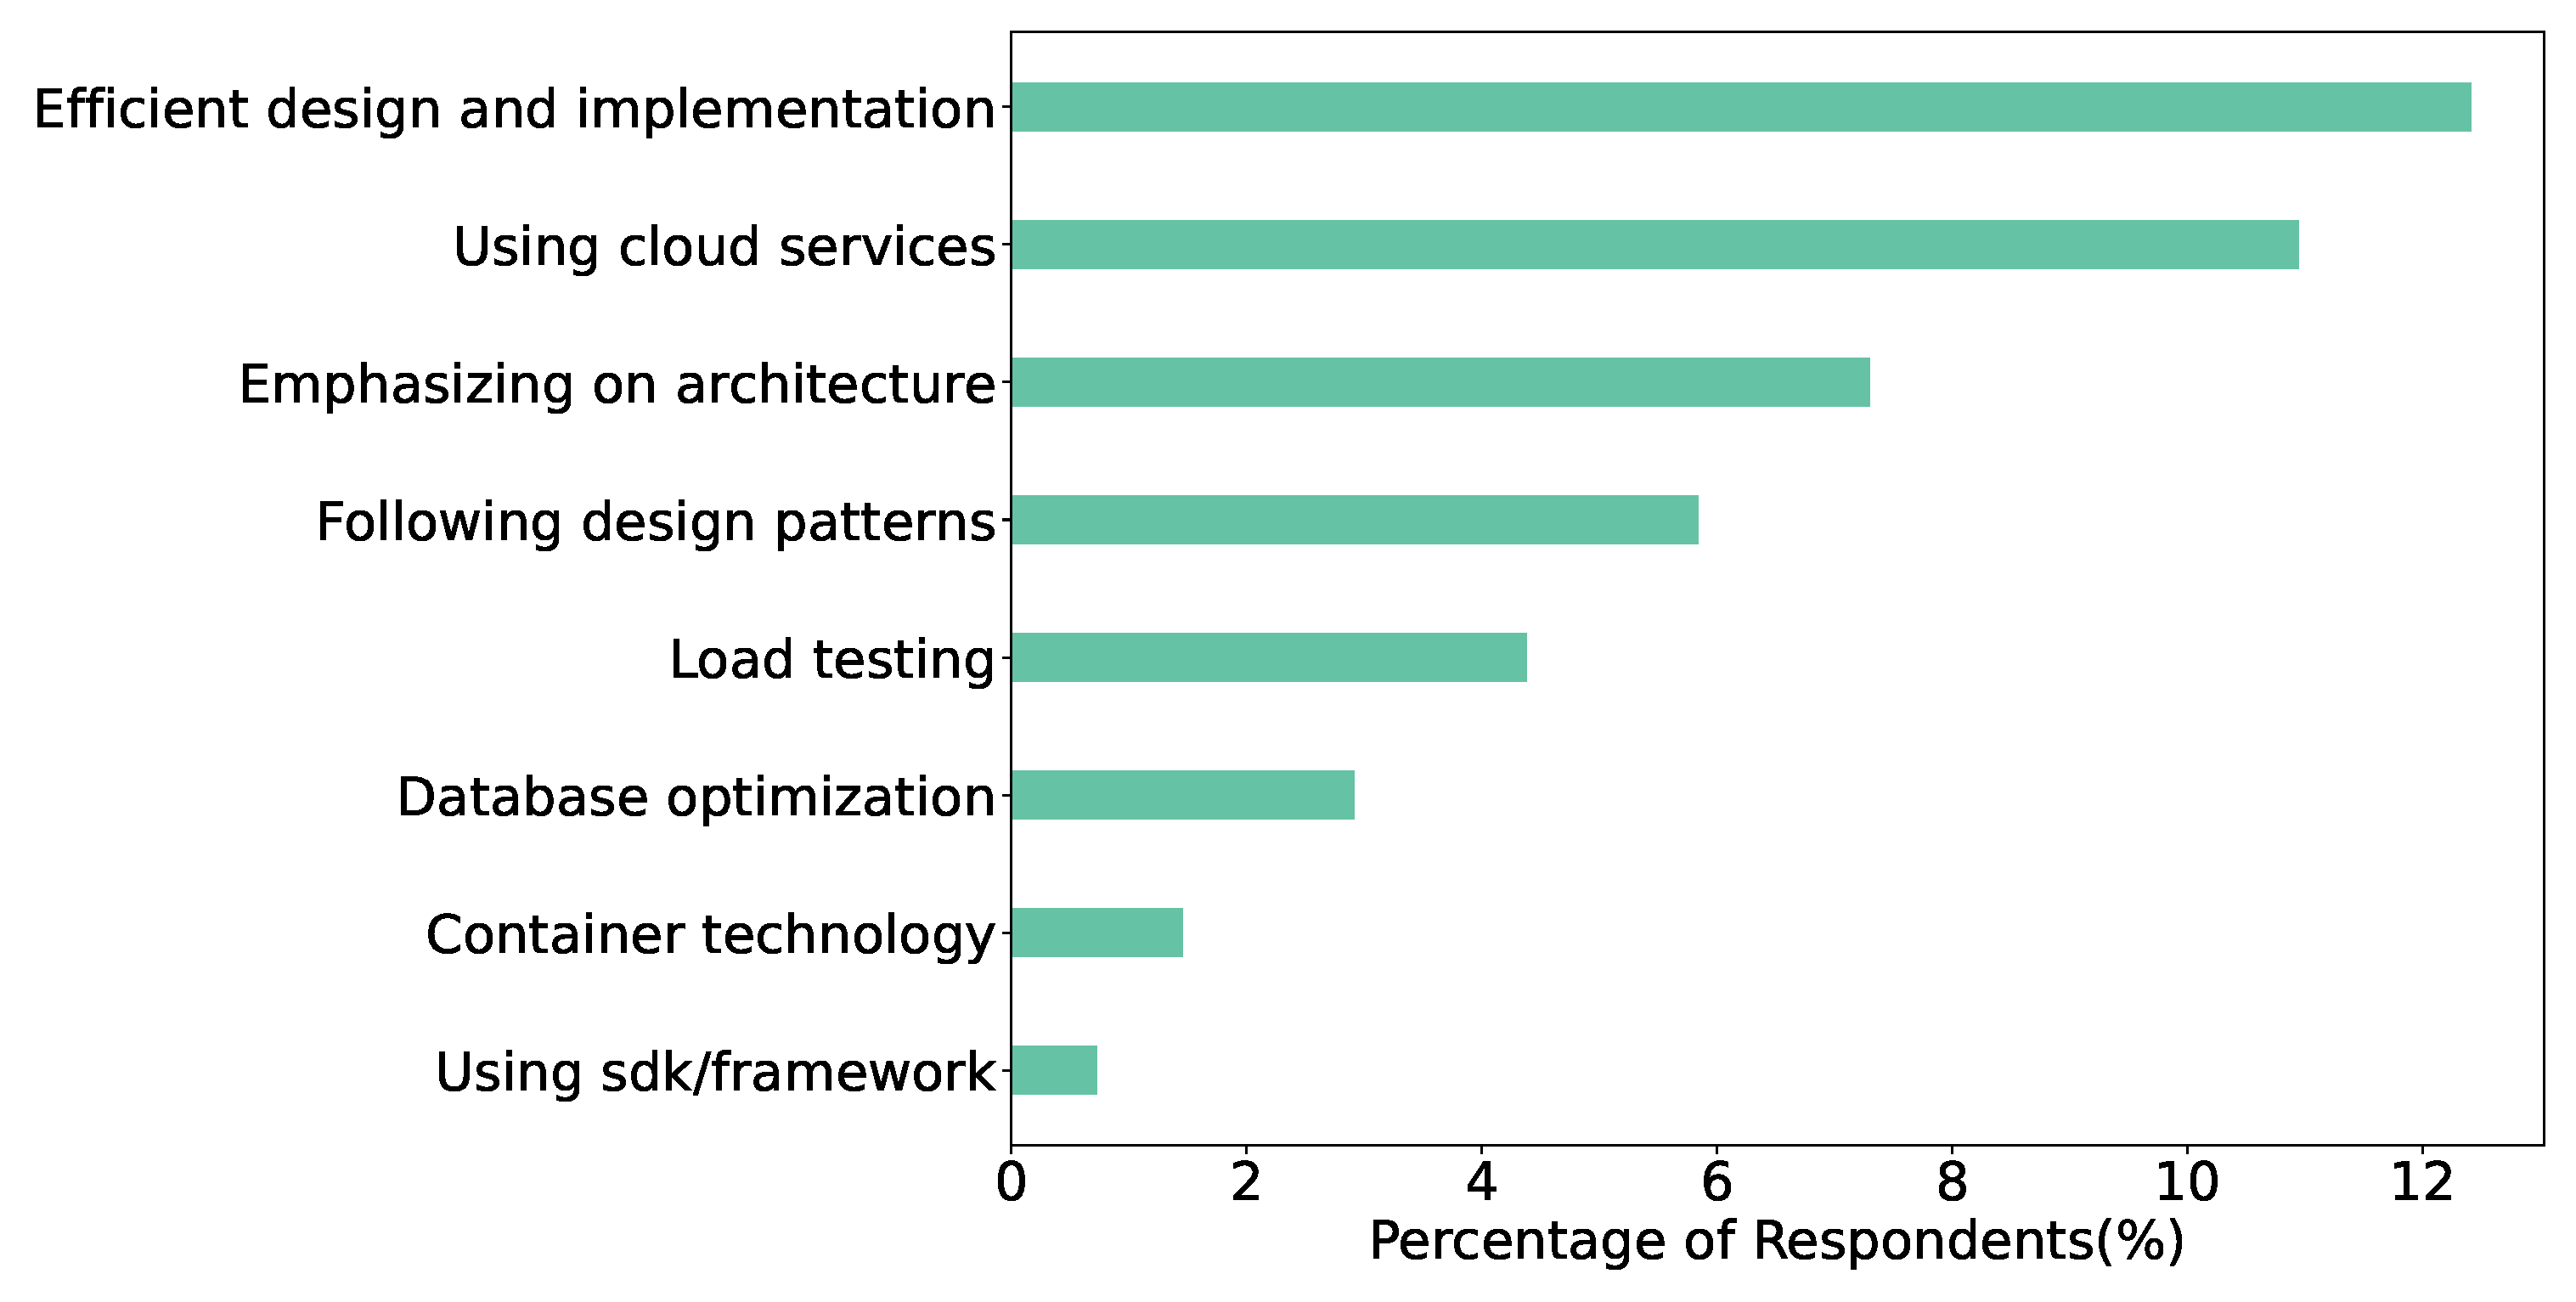
\includegraphics[scale=0.22]{Figures/Scalability.eps} 
% \caption{Measures to ensure scalability of products}
% \label{fig:Measures to ensure scalability}
% \end{figure}
% 
%  Software scalability defines the ability to scale up a solution. Issues with little importance can impede scaling up. Thus proper measures should be taken from the design stage to ensure the scalability of the system. Scalability ensured by efficient software design is the most common strategy in the Bangladesh SE industry. Our open coding of the survey responses reveals four main categories of scalability-related development practices: 
% \begin{inparaenum}
% \item Use of design principles to ensure software scalability (67.3\%).
% \item Exploitation of tools and frameworks to ensure software scalability (34.62\%). 
% \item Use of testing to ensure software scalability(11.54\%), and
% \item Use of database design standards to ensure software scalability (7.69\%).
% \end{inparaenum} 
% The measures practiced in the Bangladesh SE industry are presented in Figure \ref{fig:Measures to ensure scalability}.
% 
% 
%  Scalability ensured by efficient software design is the most common strategy in the Bangladesh SE industry. 67.3\% reported using at least one of the measures in this category. The measures in \emph{efficient software design} category are:
% % Recent days the cloud services offer tools to accomodate custom reactive scaling strategies. Thus, it has become easier to ensure scalability using cloud services \citep{Falatah2014}. Our results  also follows the world trend, usage of cloud services has placed 2\textsuperscript{nd} in terms popularity of scalability measures in SE industry of Bangladesh.
%  \begin{enumerate}[label=(\alph*)]
%  
%      \item \textbf{Efficient Design and Implementation}: 32.69\% of respondents emphasize on the design and implementation of a scalable architecture. 
%     \surveyquote{During implementation we always keep in mind about the scaling factor}{40}
%     
%      \item \textbf{Emphasizing on architecture}: 19.23\% of respondents emphasized on architecture. It is mostly micro-service architecture which they use to ensure scalability.
%     \surveyquote{We follow the micro-service architecture. In a nutshell, we scale up the module vertically which is necessary. We use docker along with Jenkins for automatic deployments and scaling.}{10}
% 
%     
%     \item \textbf{Following Design Patterns}: Some design patterns inherently help in scaling. 15.38\% of respondents think that implementing these design patterns will be of great use for software scalability.
%     \surveyquote{Following certain design patterns}{8}
%  
%  \end{enumerate}
%  
% 34.62\% of respondents of our survey use framework or tool to ensure scalability. The measures in this category are as follows:
% \begin{enumerate}[label=(\alph*)]
% 
%     \item \textbf{Using Cloud Services}: 28.85\% users depend on cloud services such as AWS and Azure for the scalability of the system. Modern features like elastic load balancing and auto-scaling make it easy to ensure scalability.
%     \surveyquote{Using AWS Elastic Load Balancer}{28}
%     
%     \item \textbf{Container Technology}: Container technologies include Docker, Kubernetes, etc. which ensure OS-level virtualization. By standardizing the system, container technologies ease the scaling of infrastructure. 3.85\% of the respondents use these measures to ensure product scalability. Containers enable users to scale their system without any dependency on the underlying OS.
%     \surveyquote{We used Docker technology}{85}
%     
%     \item \textbf{Using SDK/framework}: Modern frameworks ensure scalability by default. 1.92\% of respondents solely depend on the framework for scalability.
%     \surveyquote{following flexible framework which allows better scalability}{14}
%   
% \end{enumerate}
%  
%  
% There is one measure under the software testing category, which is load testing. Load testing can be used to check the scalability of a system. 11.54\% of respondents use load tests to check whether their system is scalable or not.
% \surveyquote{through load testing and load simulation.}{35}
% 
% There is also one measure under the Database Design category, which is database optimization. Database optimization includes sharding, clustering, indexing, and scaling. 7.69\% of respondents optimize the database to scale their system.
% \surveyquote{Besides scaling horizontally, database scaling is performed by partitioning tables, along with multi-threaded implementations}{85}
%\boxtext{Typically software scalability is considered at the design phase in the SE industry of Bangladesh.}
%\boxtext{The use of cloud services is one of the common measures to ensure scalability.}
\begin{tcolorbox}[flushleft upper,boxrule=1pt,arc=0pt,left=0pt,right=0pt,top=0pt,bottom=0pt,colback=white,after=\ignorespacesafterend\par\noindent]
\nd\it{\bf{RQ1-D4. Security and performance measures used.}} Bangladesh software
industry uses various methods to ensure security, but the adoption of tools is not widespread. 
We have noticed that the Bangladesh
software industry mostly uses performance monitoring tools and software testing
to ensure product performance. Software scalability is generally considered at
the design stage (e.g., efficient design) in the Bangladesh SE industry. 
\end{tcolorbox}

\subsection{Comparison among countries (RQ2)}
\label{RQ2}

This section presents a comparative discussion on different dimensions of software development practices and processes among different regions of the world along with Bangladesh. We make the comparison along the following dimensions:

\begin{itemize}
\item Development methods and practices
\item Implementation technologies
\item Quality assurance
\item Release and iterations
\end{itemize}

The following subsections describe these dimensions.

\subsubsection{Development methods and practices}
\label{dev_methods}

To find out the overall comparison of this section, we report the following sub-sections:

\begin{itemize}
\item Software development methodologies (Q 6).
\item Requirements gathering (Q 7).
\item Most time consuming software development activities (Q 8).
\end{itemize}

\paragraph{Software development methodologies}
From the study we see that the most acceptable model that was regularly and always used is the agile model (64\%) in Bangladesh but the usage of the scrum (44\%) in New Zealand has greater usage followed by agile (30\%) \cite{Wang2018} and in Turkey, waterfall is mostly used based on the earlier 2015 survey \cite{Garousi2015}. Again, in both Bangladesh and New Zealand, extreme programming (XP) has a lower percentage of usage.

\paragraph{Requirements Gathering}
According to \ref{fig:requirements}, using plain text (44\%) and story board (41\%) are the most widely used requirements gathering. This result is similar with the survey of Vonken et al. \cite{Vonken2012}. From their study we can find that the textual description of specifying requirements is a firm favourite in Netherlands.

\paragraph{Development activities timeline}
According to study \cite{Wang2018}, most time was spent on implementation and coding and also relatively less time was spent on maintenance in both Bangladesh and New Zealand. But requirement analysis, the activity, requires the second most time to spend in Bangladesh according to 45\% respondents where in New Zealand, it is testing (36\%) practices.

\subsubsection{Software development tools and techniques used (D2)} \label{sec:rq2-d2}
% \begin{table}[!ht]
\caption{Comparison of tech platforms, OS and programming languages between our findings and prior findings}
\begin{tabular}{llll}

\hline
\multicolumn{1}{c}{\textbf{Practices}} & \multicolumn{1}{c}{\textbf{Our Study}} & \multicolumn{1}{c}{\textbf{Prior Study}} & \multicolumn{1}{c}{\textbf{Comparison}}\\ 
\hline 


\multicolumn{1}{l|}{\multirow{3}{*}{\parbox{0.14\textwidth}{Which implementation technologies and tools are adopted by software development professionals?}}
} 

&

\multicolumn{1}{l|}{\multirow{3}{*}{\parbox{0.26\textwidth}{
\vspace{-45pt} (1) Majority of our participants were related to the various types of web-based applications that convey the market demand for web-based apps in Bangladesh. (2) Linux is mainly used for development purposes while macOS is highly preferred by managers. (3) Javascript and Java are two mostly used programming languages in the Bangladesh SE industry since the demand for web-based services as well as mobile apps.
}}} 
& 
\multicolumn{1}{l|}{\comparisoncell{0.25}{{\vspace{40pt} There exists a high level focus on web-based platforms in the software industry of New Zealand \citep{Wang2018}.
}}}
& 
\multirow{3}{*}{\parbox{0.21\textwidth}{
We have observed that web-based platforms have widespread demand among different countries along with Bangladesh. Besides, in using programming languages like Java and python, Bangladesh has similarities with Turkey but is different from New Zealand.
}} \\ \cline{3-3}

\multicolumn{1}{l|}{}                                       
& 
\multicolumn{1}{l|}{}                                       
& 

\multicolumn{1}{l|}{\comparisoncell{0.25}{{
\vspace{40pt} Windows is highly preferable among developers of New Zealand \citep{Wang2018}.
}}}                                                         
&                                                       
\\ \cline{3-3}

\multicolumn{1}{l|}{}               
& 
\multicolumn{1}{l|}{}                                        
& 

\multicolumn{1}{l|}{\comparisoncell{0.25}{
\vspace{40pt} The use of Java as a programming language is spacious in Turkey \citep{Garousi2015}. However, in New Zealand, the usage rate of Java, as well as python ranks somewhat low \citep{Wang2018}.
}} 
&                                                           
\\ \hline

\end{tabular}
\label{table:tech_comparison}
\end{table}

We compare our observations from three questions: \begin{inparaenum}
\item Technology Platform (Q9).
\item Operating System (Q10).
\item Programming Language (Q11).
%\item Framework (Q12).
%\item IDE (Q13).
\end{inparaenum} The observations from two questions (Programming language Q11 and IDE used Q12) could not be compared, because 
those were not previously asked in the context of other countries. The comparisons are discussed below.

% To find out the overall comparison of this section, we report the following sub-sections:
% \begin{itemize}
% \item Technology Platform (Q9).
% \item Operating System (Q10).
% \item Programming Language (Q11).
% \end{itemize}
% 
% We have compared our study findings on these sub-topics to get similarities and dissimilarities with the countries like Turkey, New Zealand, etc., on which a couple of relevant studies have been conducted. We compare the major findings of our study with the similar findings of previous studies in Table \ref{table:tech_comparison}.
%\paragraph{Technology Platforms}

\nd\bf{$\bullet$ Technology platforms (Q9).} As shown in
Figure~\ref{fig:platforms}, most of our survey respondents (80\%) work in web
platforms. This outcome is similar to the result of the survey of Wang et al.
\citep{Wang2018} in which the authors found that most of their respondents also
develop in web platforms in New Zealand.


%\paragraph{Operating Systems}
\nd\bf{$\bullet$ Operating Systems (Q10).} We have found an interesting point
that Windows is mostly used among developers of New Zealand based on the study
\citep{Wang2018} nevertheless, Linux is mostly used in the case for Bangladeshi
developers corresponding to our survey presented in Figure~\ref{fig:os}.

%\paragraph{Programming Languages}
\nd\bf{$\bullet$ Programming Languages (Q11).} According to the study of Wang et
al.\citep{Wang2018}, Java ranks quite low in New Zealand; nevertheless, it is
the second most used programming language in Bangladesh as per our study
reported in Figure~\ref{fig:languages} as well as the most used language in
Turkey \citep{Garousi2015}. Again, Python did not have a good standing in the
ranking of languages used in New Zealand; nevertheless, it is used significantly
in Bangladesh.

\begin{tcolorbox}[flushleft upper,boxrule=1pt,arc=0pt,left=0pt,right=0pt,top=0pt,bottom=0pt,colback=white,after=\ignorespacesafterend\par\noindent]
\nd\it{\bf{RQ2-D2. Software development tools and techniques used.}}
Like other SE industries, the web is the main technology platform in Bangladesh.
Linux is the preferred OS in Bangladesh's SE industry, while it is  Windows in 
New Zealand SE industry. Although Java and Python are popular languages in the
SE industry in Bangladesh, we have noticed that they are not very popular in the
New Zealand SE industry.
\end{tcolorbox}
\subsubsection{What type of testing and deployment practices are used?}

To get the picture of quality assurance (QA) in countries such as Malaysia, Turkey, France, etc., different studies have been carried out. In Table \ref{table:testing_comparison}, we compare the major outcomes of testing and deployment related responses from our study with the similar results of the previous studies. The comparative picture is discussed below.

\begin{itemize}
    % \item Requirements Clarity
    \item Software Testing Practices (Q14)
    \item Level of Automated Testing (Q15)
\end{itemize}

\begin{table}[]
\caption{Comparison of testing practices and test automation between our findings and prior findings}

\begin{tabular}{llll}

\hline
\multicolumn{1}{c}{\textbf{Practices}} & \multicolumn{1}{c}{\textbf{Our Study}} & \multicolumn{1}{c}{\textbf{Prior Study}} & \multicolumn{1}{c}{\textbf{Comparison}} \\ 
\hline 


\multicolumn{1}{l|}{\multirow{2}{*}{\parbox{0.1\textwidth}{What type of testing and deployment practices are used?}}
} 
& 
\multicolumn{1}{l|}{\multirow{2}{*}{\parbox{0.25\textwidth}{
\vspace{-50pt} (1) Around half of our respondents responded about carrying out unit testing and functional testing. Also, the utilization rate of acceptance and UI testing has an appreciable percentage in Bangladesh. (2) Automated testing exercise is not usual in Bangladesh as per the majority of our respondents.
}}
} 
& 
\multicolumn{1}{l|}{\comparisoncell{0.25}{\vspace{50pt}Unit testing is observed to be the most exercised in Malaysia (68.29\%) \citep{Baharom2006}, Canada (79.27\%) \citep{Garousi2013}, New Zealand (73\%) \citep{Wang2018} in a great percentage.
}}                                  

&

\multirow{2}{*}{\parbox{0.23\textwidth}{
\vspace{-70pt} We have perceived that unit testing is moderately practiced in Bangladesh, though its usage is comparatively spacious in other countries. In the adoption of test automation, the software industry of Bangladesh is way behind France though the usage rate might have similar to other European countries.
}} \\ \cline{3-3}

\multicolumn{1}{l|}{}                                       
& 
\multicolumn{1}{l|}{}                                       
& 

\multicolumn{1}{l|}{\comparisoncell{0.25}{
\vspace{50pt} Test automation is highly embraced by France software industry and comparatively less adopted in overall Europe~\citep{dutta1999}.
}} 
&                                         
\\ \hline

\end{tabular}
\label{table:testing_comparison}
\end{table}



\paragraph{Software Testing Practices}
From our study, as per \ref{fig:testing}, we see an interesting point that unit testing (53\%) and functional testing (49\%) are moderately used in Bangladesh, whereas from \citep{Garousi2013} and \citep{Wang2018} we can see that relatively a high percentage of their survey respondents in both Canada New Zealand rely on unit testing with 79.27\% and 73\% respectively. On the other hand, the adoption of acceptance testing and UI testing is quite similar to these countries. In Malaysia, based on \citep{Baharom2006}, Baharom et al. reported that, according to their survey, unit testing (68.29\%), integration testing (78.05\%), system testing (85.37\%), and acceptance testing (78.05\%) are used by most organizations in a high percentage, and about half of the organizations are carrying out alpha and beta testing.

\boxtext{Software developers around the world usually give unit testing the top priority, but the developers in Bangladesh have comparatively less participation.}
\rifat{Is the above observation correct? 53\% usage of unit testing reported.}\khalid{added percentages. The response rate of unit testing in our survey lags compares to others. Is it okay now?}

\paragraph{Level of Automated Testing}
We have found that as per \ref{fig:autoTest}, around 25\% of our respondents are highly concerned that they have to use automated testing for their projects, while around 35\% of our respondents have expressed medium level concern and the remaining are hardly concerned about using automated testing. From the study of Dutta et al. \citep{dutta1999}, we have found that in automated testing practices, Bangladesh is quite similar to all of Europe but lags behind France. According to their study, the usage rate of automation testing tools in overall Europe is 26\%, where in France, it is as high as 61\%. But in Israel, this rate is the only 9\%.

\begin{tcolorbox}[flushleft upper,boxrule=1pt,arc=0pt,left=0pt,right=0pt,top=0pt,bottom=0pt,colback=white,after=\ignorespacesafterend\par\noindent]
\nd\it{\bf{RQ2-D3. Software testing and devops practices used.}} 
\gias{summarize}
\end{tcolorbox}

% \subsubsection{Release and Iterations}
\label{vcs_comparison}

\subsubsection{How are the security and performance ensured in the products of a company?}

Several studies have been performed to identify security and performance practices in countries like Canada, New Zealand, and Turkey. We have found some differences as well as similarities in the practices of those countries with others. In Table \ref{table:open_ended_comparison}, we compare the major findings of our study against the findings of previous studies.

% Please add the following required packages to your document preamble:
% \usepackage{multirow}
\begin{table}[!ht]
\caption{Comparison of security, performance, scalability between our findings and prior findings}
\begin{tabular}{llll}

\hline
\multicolumn{1}{c}{\textbf{Practices}} & \multicolumn{1}{c}{\textbf{Our Study}} & \multicolumn{1}{c}{\textbf{Prior Study}} & \multicolumn{1}{c}{\textbf{Comparison}} \\ 
\hline

\multicolumn{1}{l|}{\multirow{3}{*}{\parbox{0.1\textwidth}{
How are the security and performance is ensured in a product of a company?
}}}

&

\multicolumn{1}{l|}{\multirow{3}{*}{\parbox{0.22\textwidth}{
(1) The practice of security architecture and security testing as a security measure are not prevalent in the Bangladesh SE industry. (2) Performance testing and peer review are the two least practiced performance measure in the Bangladesh SE industry. (3) Cloud service and architecture are two of the top three scalability measures.
}}} 

&

\multicolumn{1}{l|}{\comparisoncell{0.30}{
\vspace{13pt} Security testing is found to be the least practiced in the software industry in Turkey\citep{Garousi2015}, Malaysia\citep{Farvin2016}, India\citep{Bahl2011}, and New Zealand\citep{Sung2006}
}}                                                          

& 

\multirow{3}{*}{\parbox{0.22\textwidth}{
We found that the practice of `no security' measures is less in Bangladesh compared to other countries. Though the practice of security testing Bangladesh has similarities with other countries, it lags behind the practices of matured industries. However, like the matured and grown software industries, cloud service is a popular measure in Bangladesh.
}} 
\\ \cline{3-3}

\multicolumn{1}{l|}{}                                       
& 
\multicolumn{1}{l|}{}                                       
&

\multicolumn{1}{l|}{\comparisoncell{0.30}{
\vspace{13pt} Performance testing is a common practice in some \citep{Garousi2013,Garousi2015,Phillips2003} SE industry. However, it is hardly practiced in the Pakistan\citep{Jahan2019} SE industry. Also, peer review is a common practice among Turkish\citep{Garousi2015} developers.
}}                                                          

& 
\\ \cline{3-3}
\multicolumn{1}{l|}{}                                       
& 
\multicolumn{1}{l|}{}  
& 

\multicolumn{1}{l|}{\comparisoncell{0.30}{
\vspace{13pt} To ensure scalability, there are many practices prevalent in other countries' SE industry, such as micro-service architecture\citep{Laihonen2018} and containerization technologies\citep{Hussain2017}.
}} 
& 
\\ \hline


\end{tabular}
\label{table:open_ended_comparison}
\end{table}

\label{security_comparison}
A very few percentages (3.64\%) of our survey respondents reported not to use any security measures in their product. This practice is also prevalent in the Indian and Malaysian software industries. Bahl et al.\citep{Bahl2011} reported that due to misalignment with organization design, goal, and strategy in some Indian software firms, security measures are not practiced. In a study with Malaysian developers, Farvin et al.\citep{Farvin2016} found that 31\% of respondents think it is not required to add security in the requirement analysis of a product. Basharat et al.\citep{Basharat2013} reported a sense of false security in the small software industry and standard security practices are hardly followed. It is likely to be applicable to the industry in Bangladesh as well. From the response of a survey on the Turkish software industry, Garousi et al.\citep{Garousi2015} ranked different design activities in terms of frequency. Security architecture was ranked second out of five (five is for always used activities and one is for never used activities). The ranking represents that security architecture is not a frequent activity in the Turkish software industry. However, in our survey, we see very few respondents reported to practice security design principles while designing system architecture. Our survey found that 2.19\% of respondents rely on security architecture/security design principles to ensure security in their product. The software industries of Bangladesh, Turkey, and New Zealand have a resemblance in the practice of security testing. Garousi et al.\citep{Garousi2015} reported that security testing is least widely used among all kinds of testing (e.g., unit testing, integration testing). Sung et al.\citep{Sung2006} found that in the New Zealand software industry, security testing and recovery testing practices are negligible compared to functional testing. The scenario is the same for Bangladesh; we found that 6.57\% of respondents reported security testing to ensure security.


% \subsubsection{Performance measures}
% \label{performance_comparison}
8.76\% respondents of our survey use performance testing to ensure the performance of their product. \anindya{Should we say respondents or the companies they work? Think about it as we mention this at different places.}\partha{The survey question was `How do you ensure security of your products?' participants may answer this question from both personal and company perspective. It seems to me that the goal was to find out the participants' security practices. What do you suggest?} However, it is the second least practiced measure among all the measures. Garousi et al.\citep{Garousi2015} found that developers mark the lack of performance testing as the main challenge in software maintenance in the Turkish software industry. However, the scenario is different for the Canadian software industry. Participants of the survey of Garousi et al.\citep{Garousi2013} reported that 40\% of them conduct performance testing, and 30\% of their total testing effort is spent on performance testing. The New Zealand software industry follows the practice similar to Canada as reported by Phillips et al.\citep{Phillips2003}. %reported that performance testing is a common testing practice in New Zealand.
The practice in Bangladesh matches that of Pakistan. 
%In Pakistan software industry, performance testing is hardly practiced.
In the survey of Shah Jahan et al.\citep{Jahan2019}, only 5\% of participants reported conducting performance testing. It seems that performance testing is less popular in growing software industries such as Bangladesh and Pakistan.

Peer review is the least practiced measure in the Bangladesh software industry. However, in the Turkish software industry, peer review is ranked as the most frequent activity\citep{Garousi2015} (ranked five on a five-point Likert scale), though the practice is only limited to code review. Architecture/design review is hardly practiced in turkey (ranked one on a five-point Likert scale). We found that peer review is limited to only code review in the Bangladeshi software industry, and the only 2.92\% of our participants reported practicing peer review.

% \subsubsection{Scalability measures}
% \label{scalability_comparison}
There is no study focusing on scalability practices in specific software industries, so it isn't easy to compare scalability practices. However, in a study on Finnish DevOps, Laihonen\citep{Laihonen2018} found that the Finnish software industry prefers cloud services as it helps them automate quality assurance. He also reported that DevOps is inclined towards micro-service architecture when selecting a product rather than monolithic architecture. Hussain et al.\citep{Hussain2017} conducted a study to identify trends in the DevOps practices in New Zealand. For this study, besides interviewing the DevOps, they examined the job advertisements for a DevOps role. They found that containerization technologies (e,g., Docker, Kubernetes) have a high demand in the New Zealand software industry. 94\% of job advertisement requires expertise in one or multiple containerization technologies. This indicates the popularity of docker technology in the New Zealand software industry. However, in the Bangladeshi software industry, the scenario is different. Cloud services are the second most popular (10.95\%) measure to ensure scalability where the use of containerization technologies are not that much popular (1.46\%)

\begin{tcolorbox}[flushleft upper,boxrule=1pt,arc=0pt,left=0pt,right=0pt,top=0pt,bottom=0pt,colback=white,after=\ignorespacesafterend\par\noindent]
\nd\it{\bf{RQ2-D4. Security and performance measures used.}} \gias{summarize RQ2-D4 here}
\end{tcolorbox}




% \subsection{Development Practices and Processes in Bangladesh (RQ1)}
\label{RQ1}

We divide this into following four sub-questions which examine software development practices and processes in Bangladesh in more detail.

\subsubsection{What software methodology are used in your project?}
\label{methodology}
Software development methodology in software engineering is a framework that is used to pursue the development of information systems in a very deliberate, structured and methodical way. To find out the overall answer of this question, we report the following results:
\begin{itemize}
\item Software development methodologies (Q 6).
\item Requirements gathering (Q 7).
\item Most time consuming software development activities (Q 8).
\end{itemize}

\paragraph{Software development methodologies}
The most-widely used model is Agile with usage rate of 64\%. The next widely-used model is scrum with usage rates of 46\%. The other methodologies has lower usage rates, namely: pair programming (20\%), Waterfall (12\%) etc.

% \begin{figure}[htbp]
% \centering
%   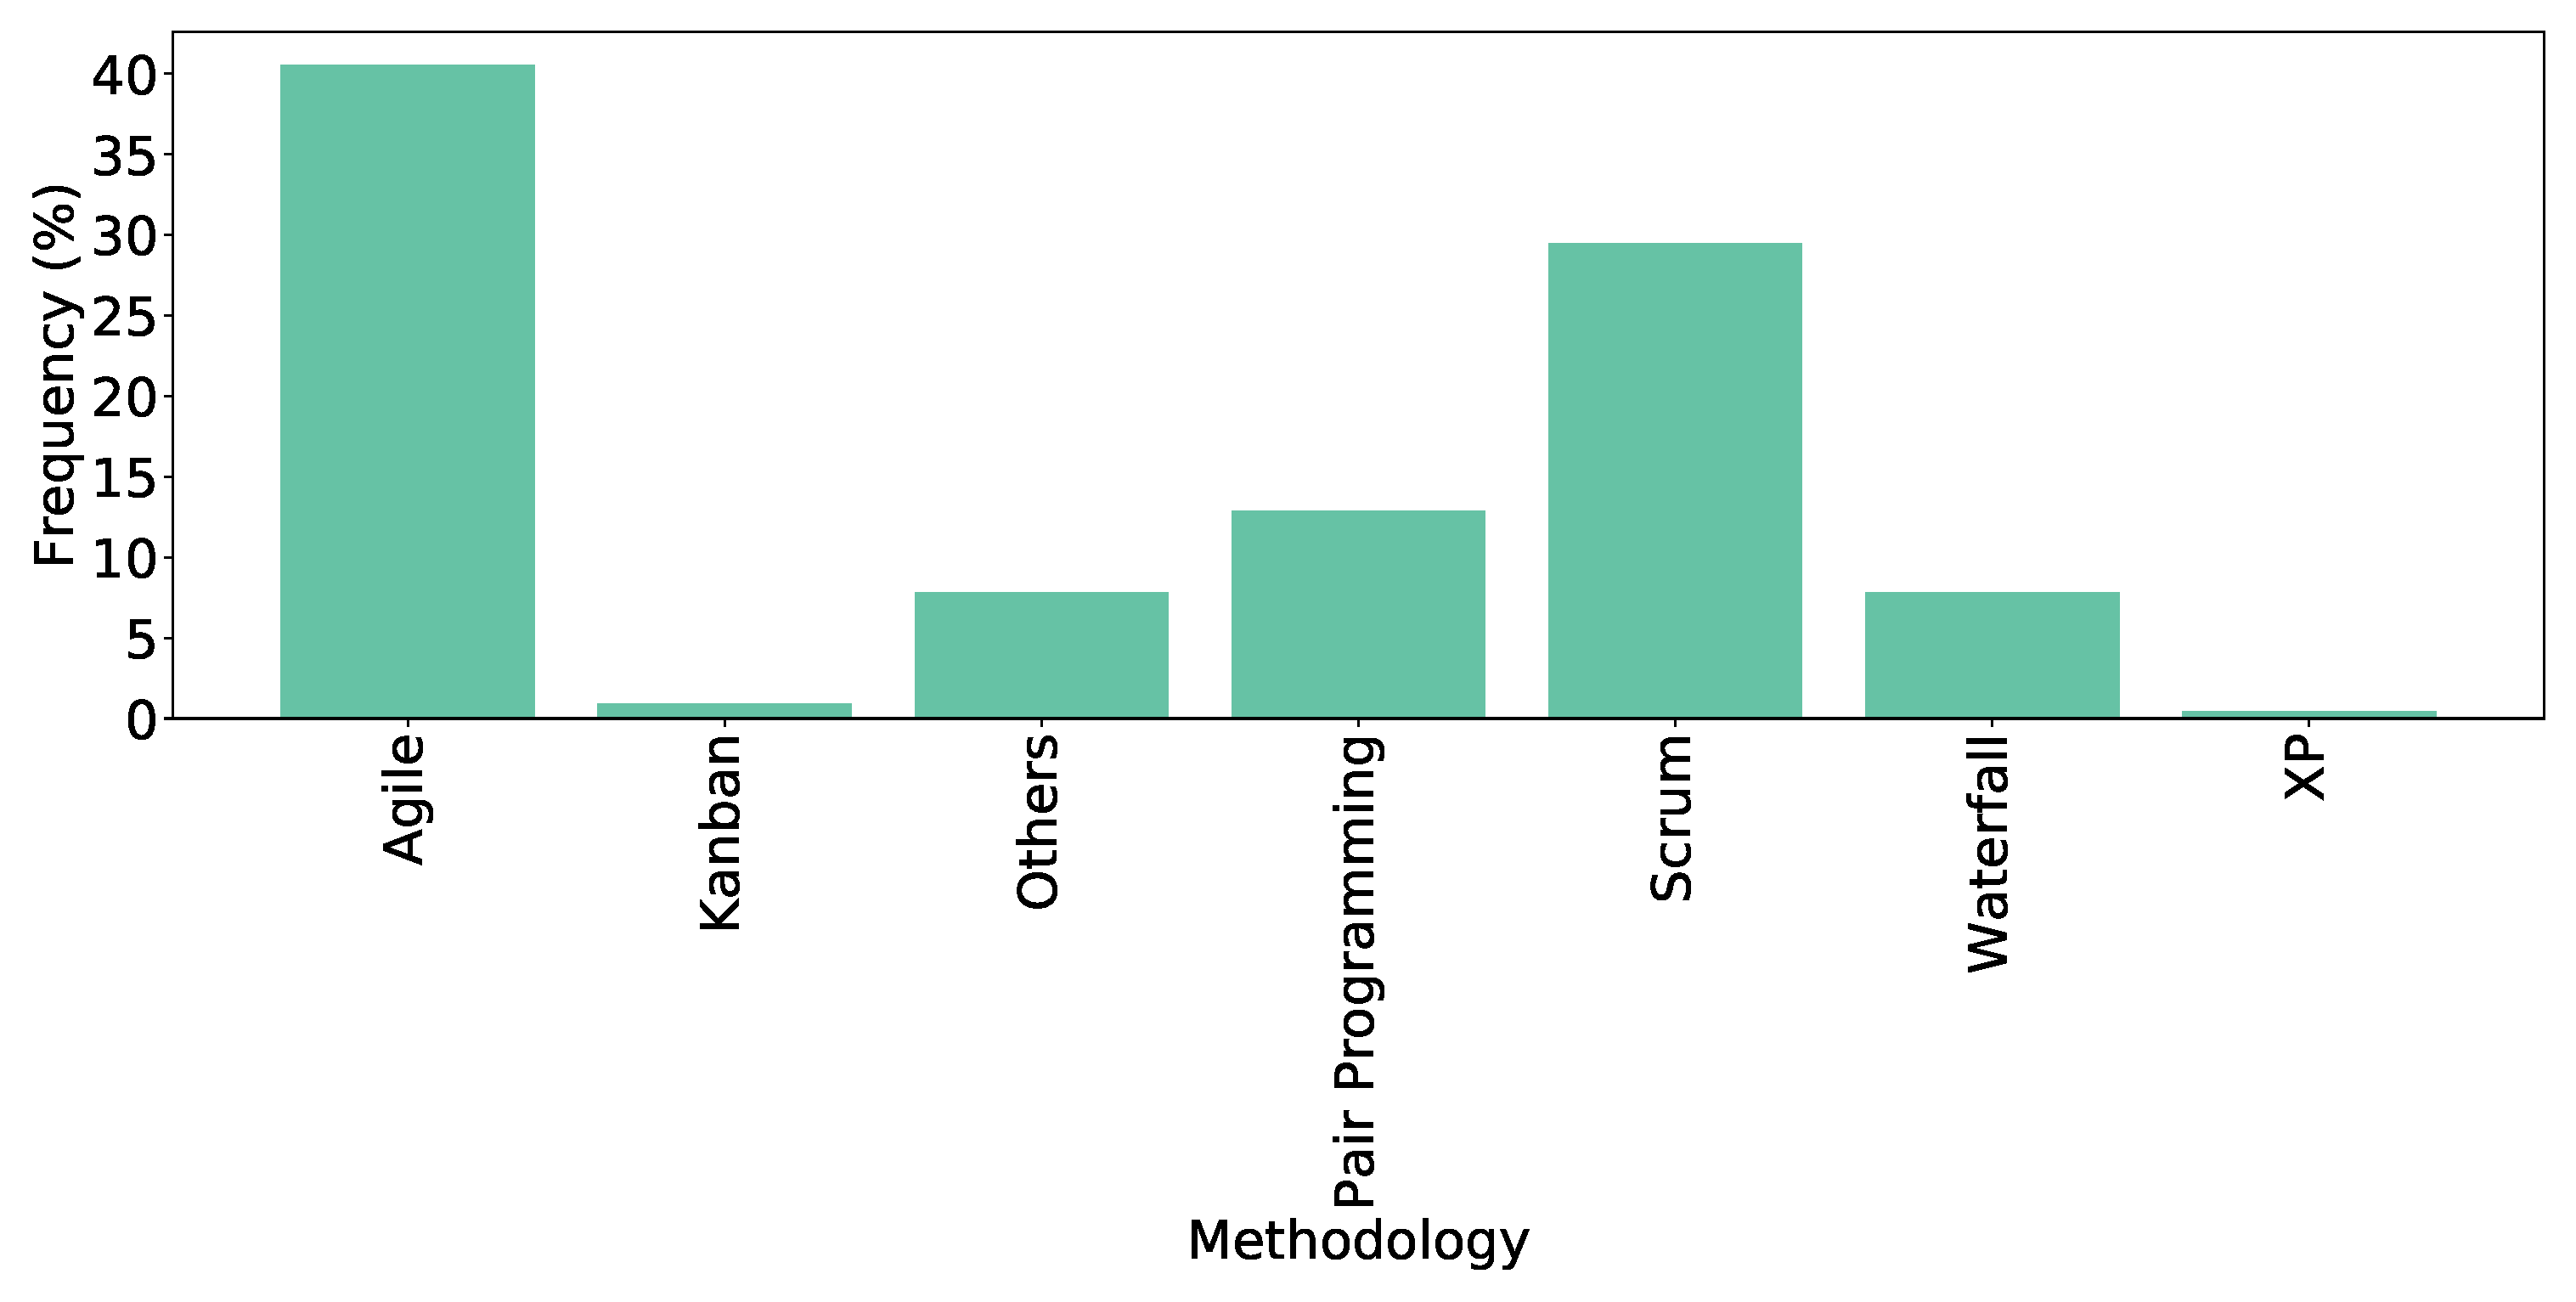
\includegraphics[width=0.8\textwidth]{Figures/Respondents_Methodology}
%   \caption{Software development methodologies}
%   \label{fig:methodologies}
% \end{figure}

\paragraph{Requirements Gathering}
The most critical activity that always arises during software development is the collecting requirement of the proposed system. According to \ref{fig:requirements}, using plain text (44\%) and story board (41\%) are the most widely used requirements gathering. The other requirements gathering usage rates are: Use case (36\%), GUI prototype (35\%), grooming session (30\%) etc. This is an important finding that requires further analysis for causes and to analyze the potential effects of not documenting requirements.

% \begin{figure}[htbp]
% \centering
%   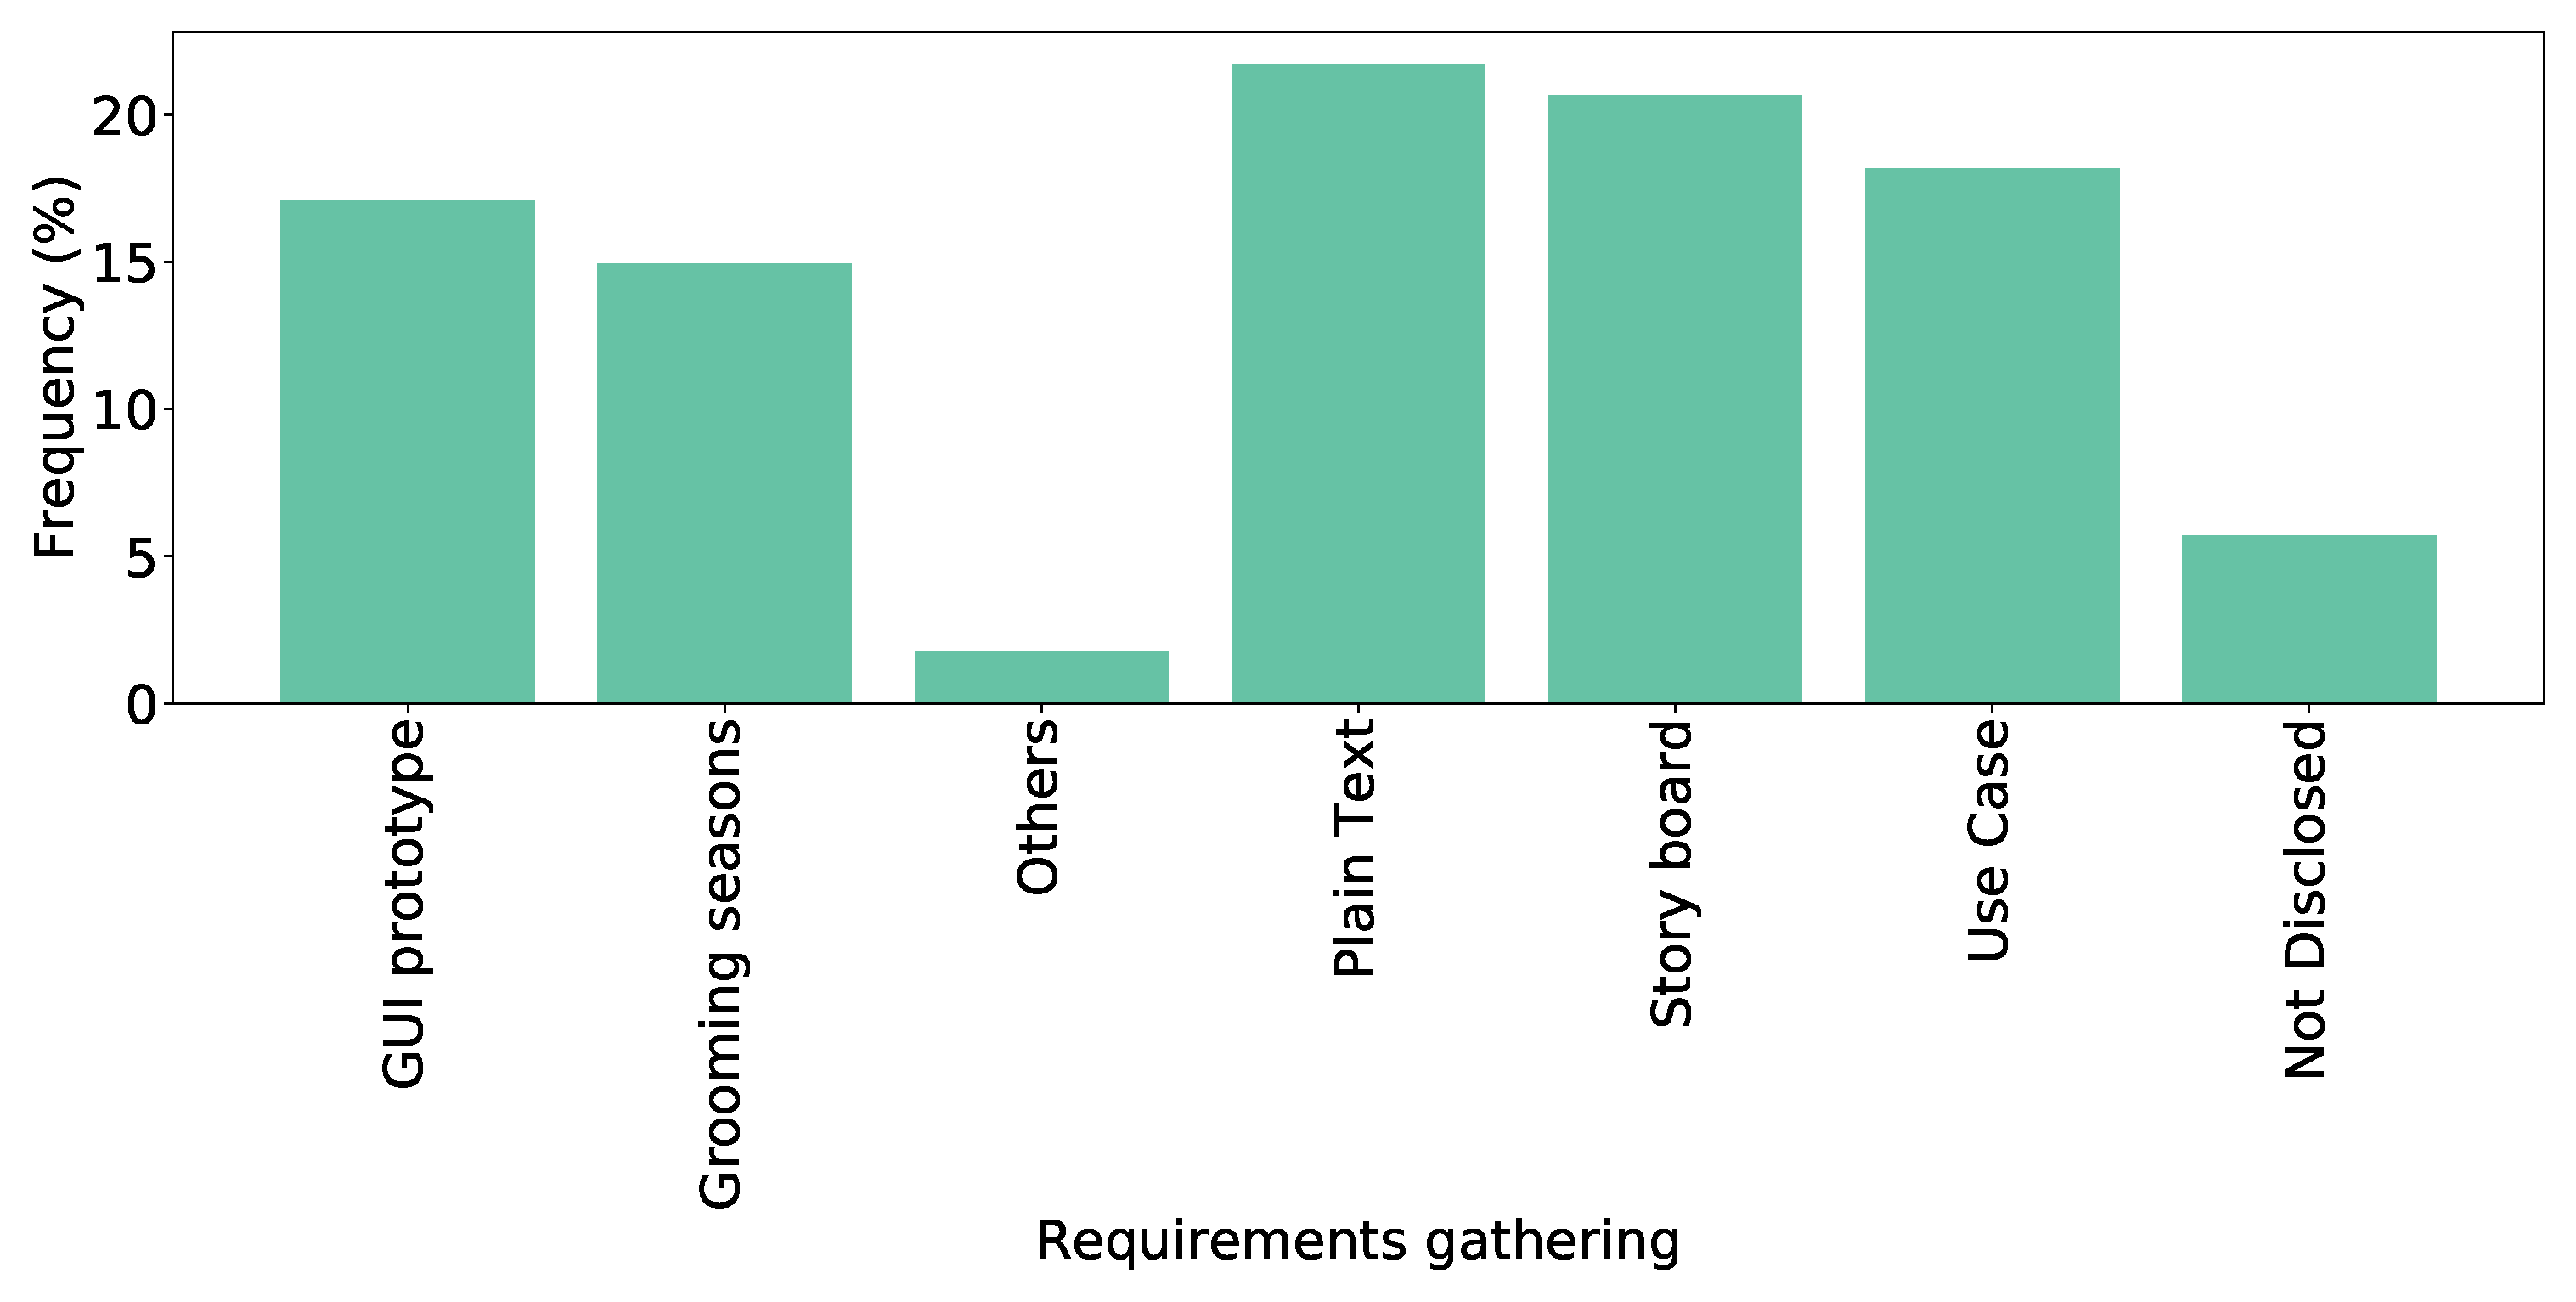
\includegraphics[width=0.8\textwidth]{Figures/Requirements_Gathering}
%   \caption{Requirements gathering}
%   \label{fig:requirements}
% \end{figure}

\paragraph{Development activities timeline}
In this section participants were asked about the most time consuming software developing activities they had spend. As we see in \ref{fig:activities}, most of the time spent in implementation stage according to 65\% our respondents and requirement analysis stage requires second most according to 45\% response. The other usages are: Program design (37\%), project planning (30\%), testing (19\%), maintenance (17\%) etc.

% \begin{figure}[htbp]
% \centering
%   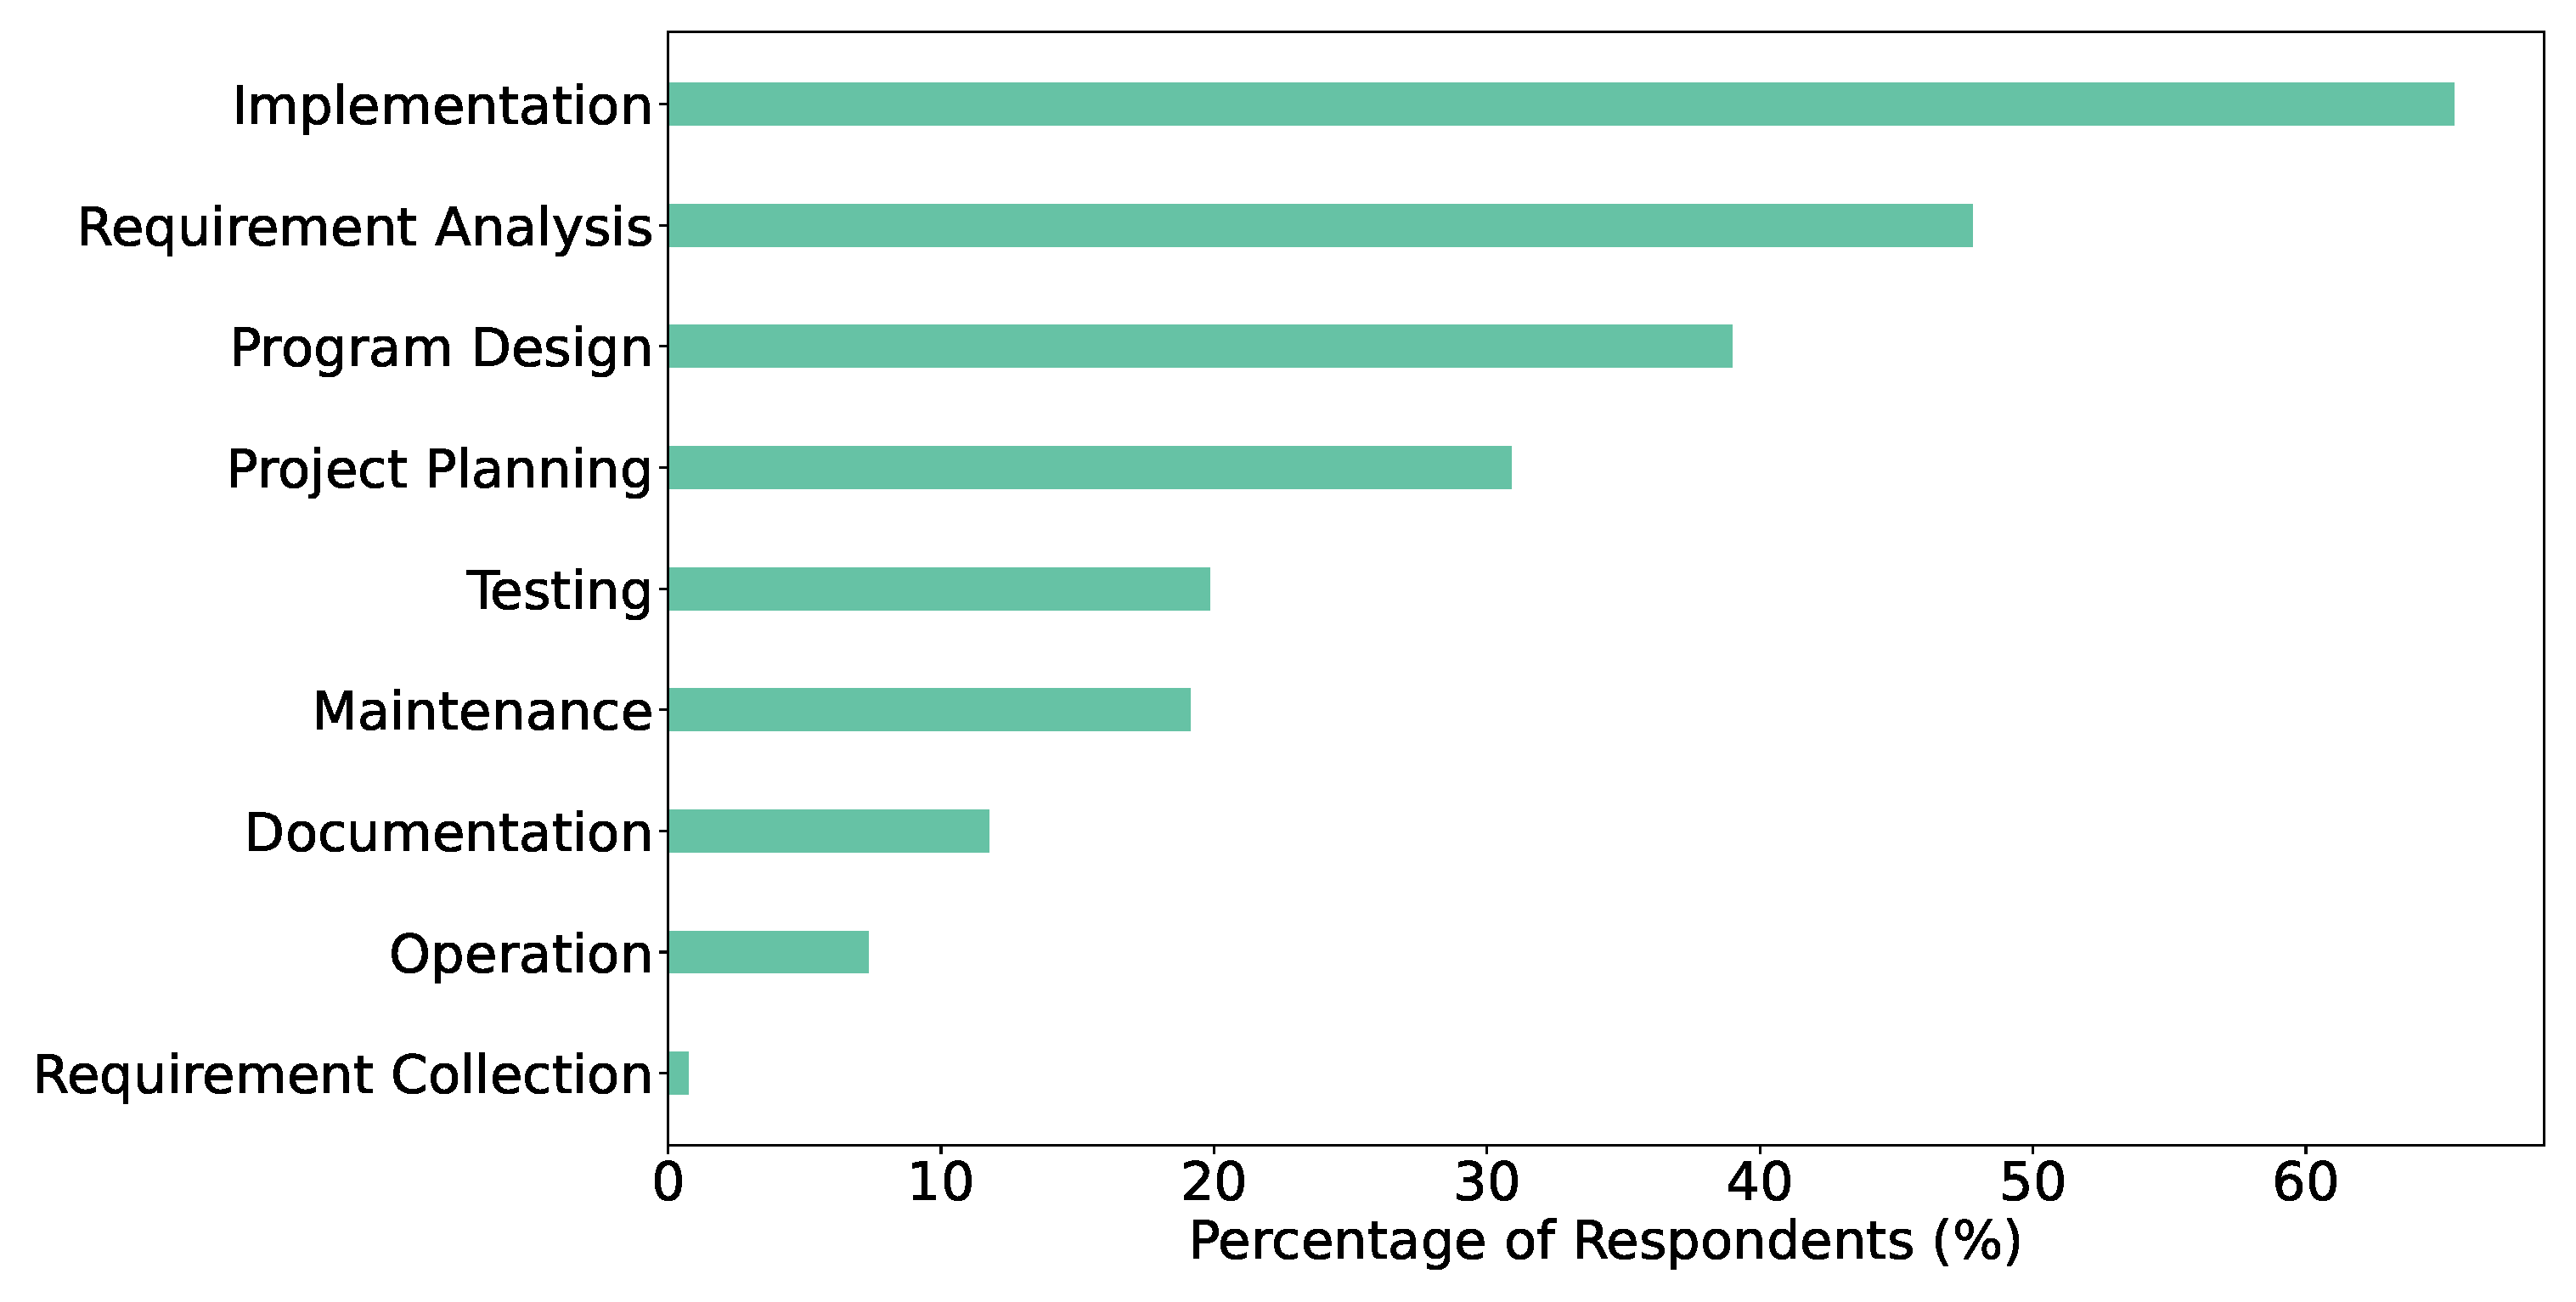
\includegraphics[width=0.8\textwidth]{Figures/Respondents_Activities}
%   \caption{Software development activities}
%   \label{fig:activities}
% \end{figure}


\subsubsection{Which implementation technologies and tools are adopted by software development professionals?}
\label{tools}

Our survey included five questions to find technologies and tools that are adopted by software development professionals. To answer this question fully, we report the following results:
\begin{itemize}
\item Technology Platform (Q 9).
\item Operating System (Q 10).
\item Programming Language (Q 11).
\item Framework (Q 12).
\item IDE (Q 13).
\end{itemize}

\paragraph{Technology Platforms}
Participants were allowed to choose multiple options. As shown in \ref{fig:platforms}, most of the respondents (80\%) worked in web platform. The rests were mobile (45\%), Desktop (30\%), Embedded/IOT (8\%).
% \begin{figure}[htbp]
% \centering
%   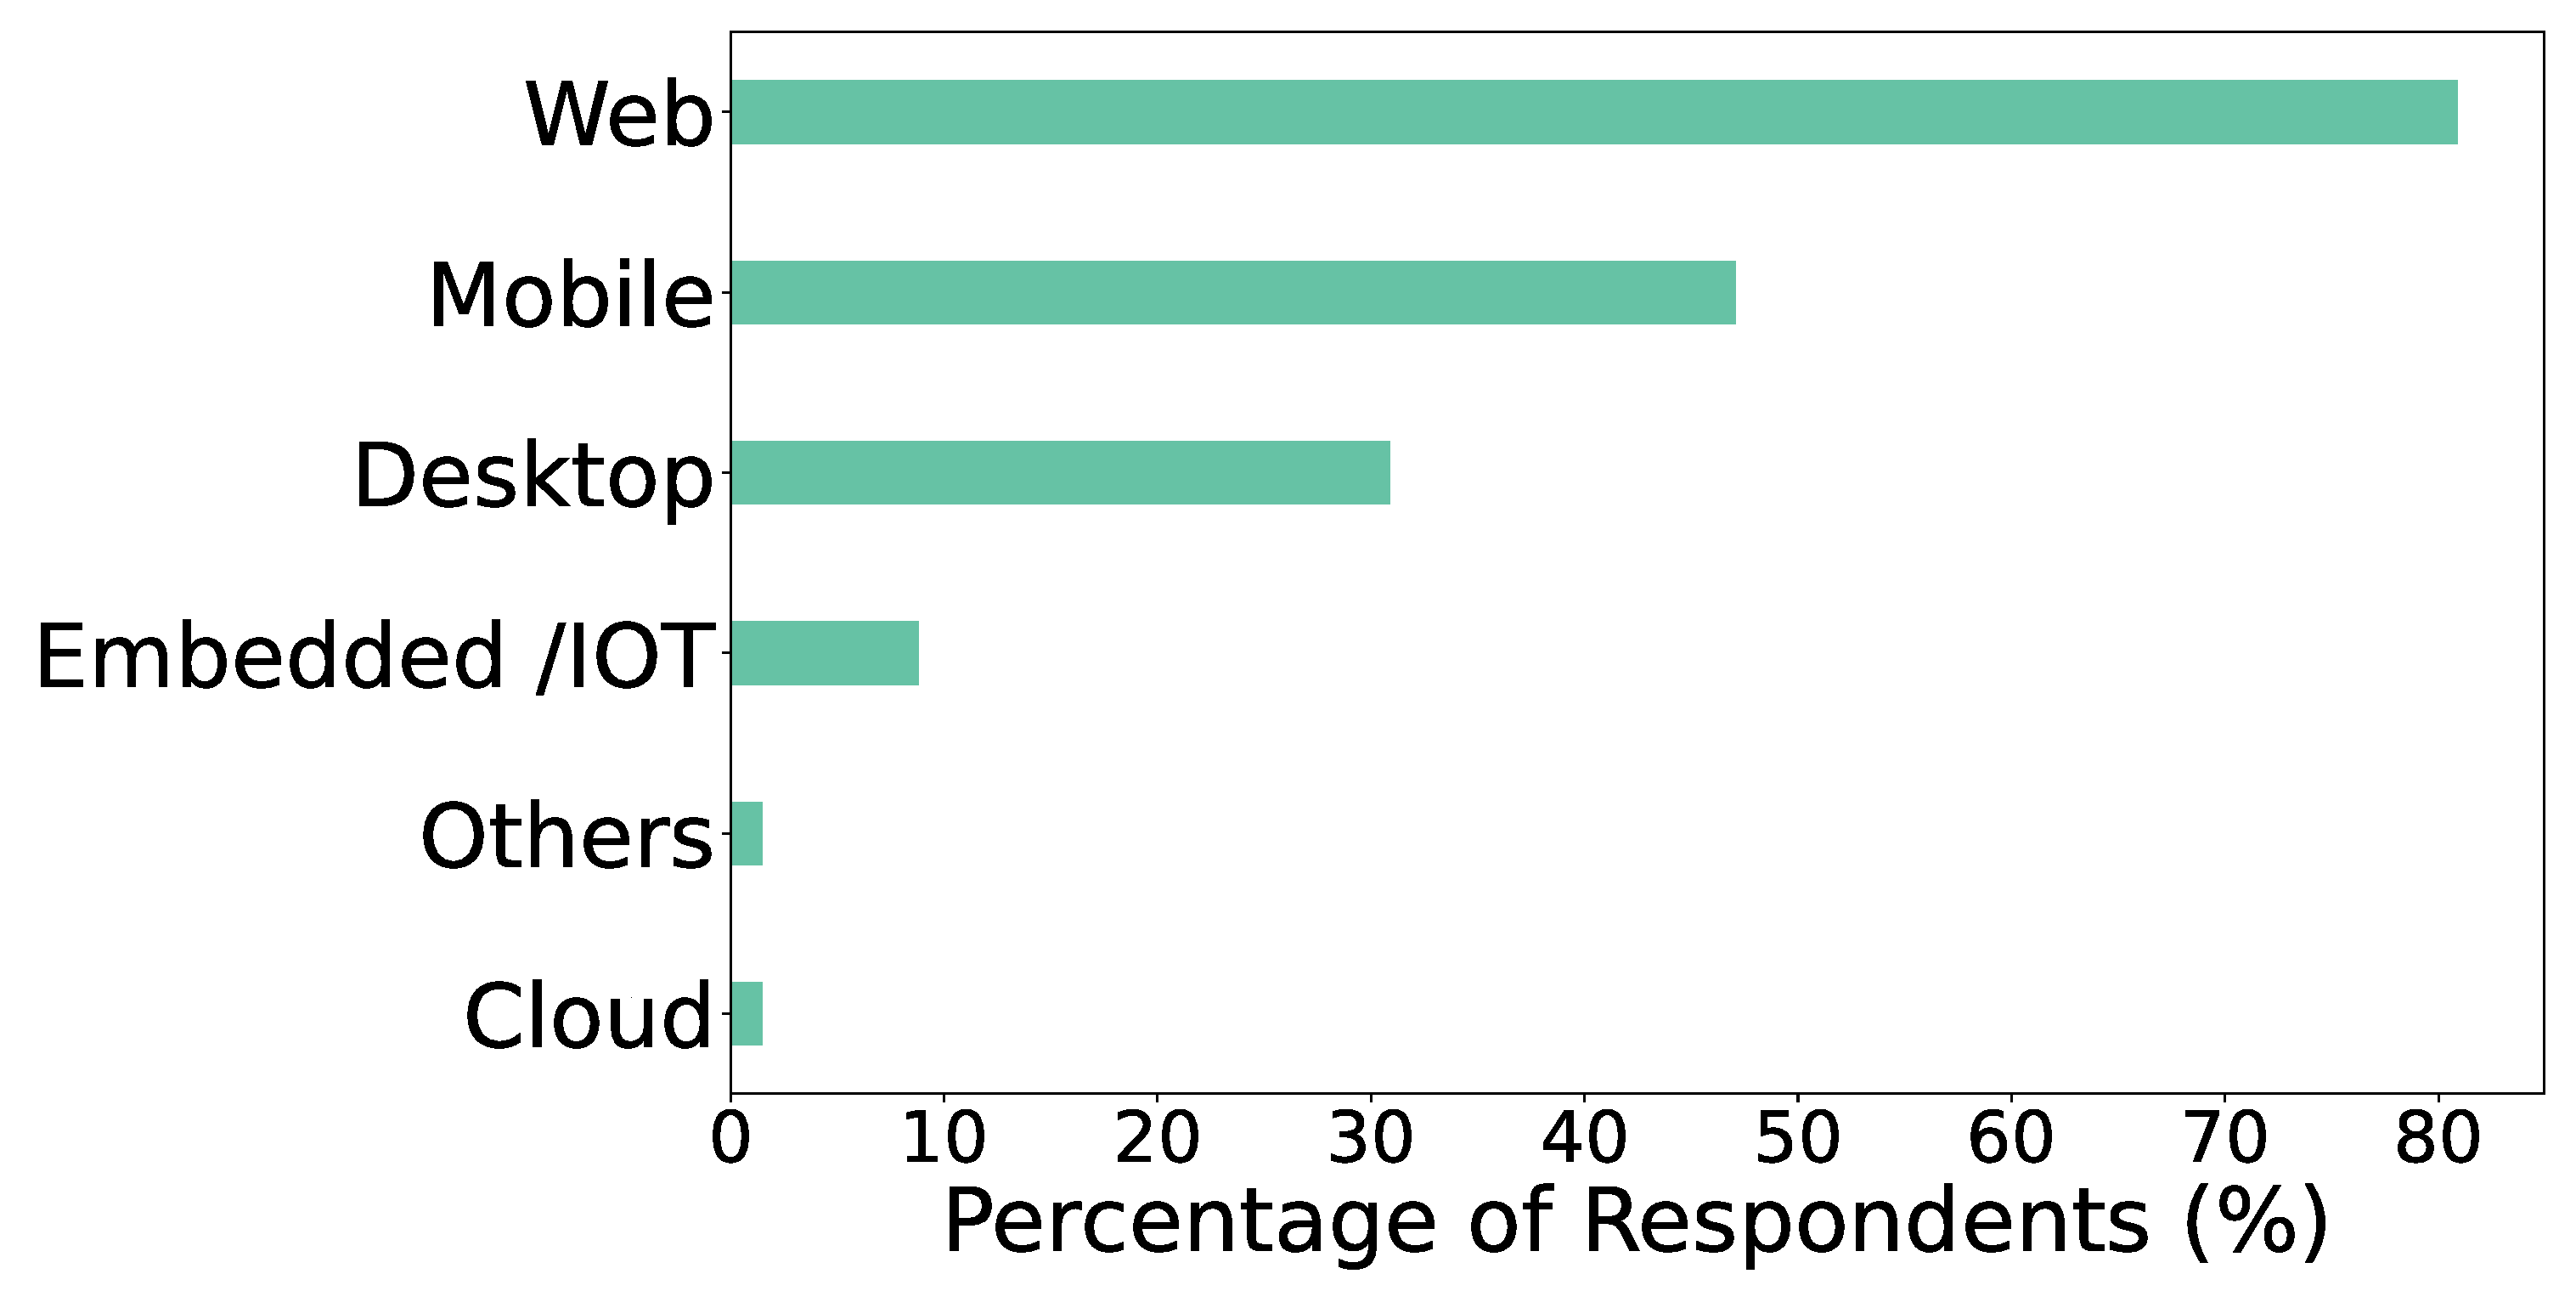
\includegraphics[width=0.8\textwidth]{Figures/Respondents_Technologies}
%   \caption{Technology Platforms}
%   \label{fig:platforms}
% \end{figure}

\paragraph{Operating Systems}
Most of our respondent's used linux based operating system (56\%). The second best used operating system is windows (45\%).

% \begin{figure}[htbp]
% \centering
%   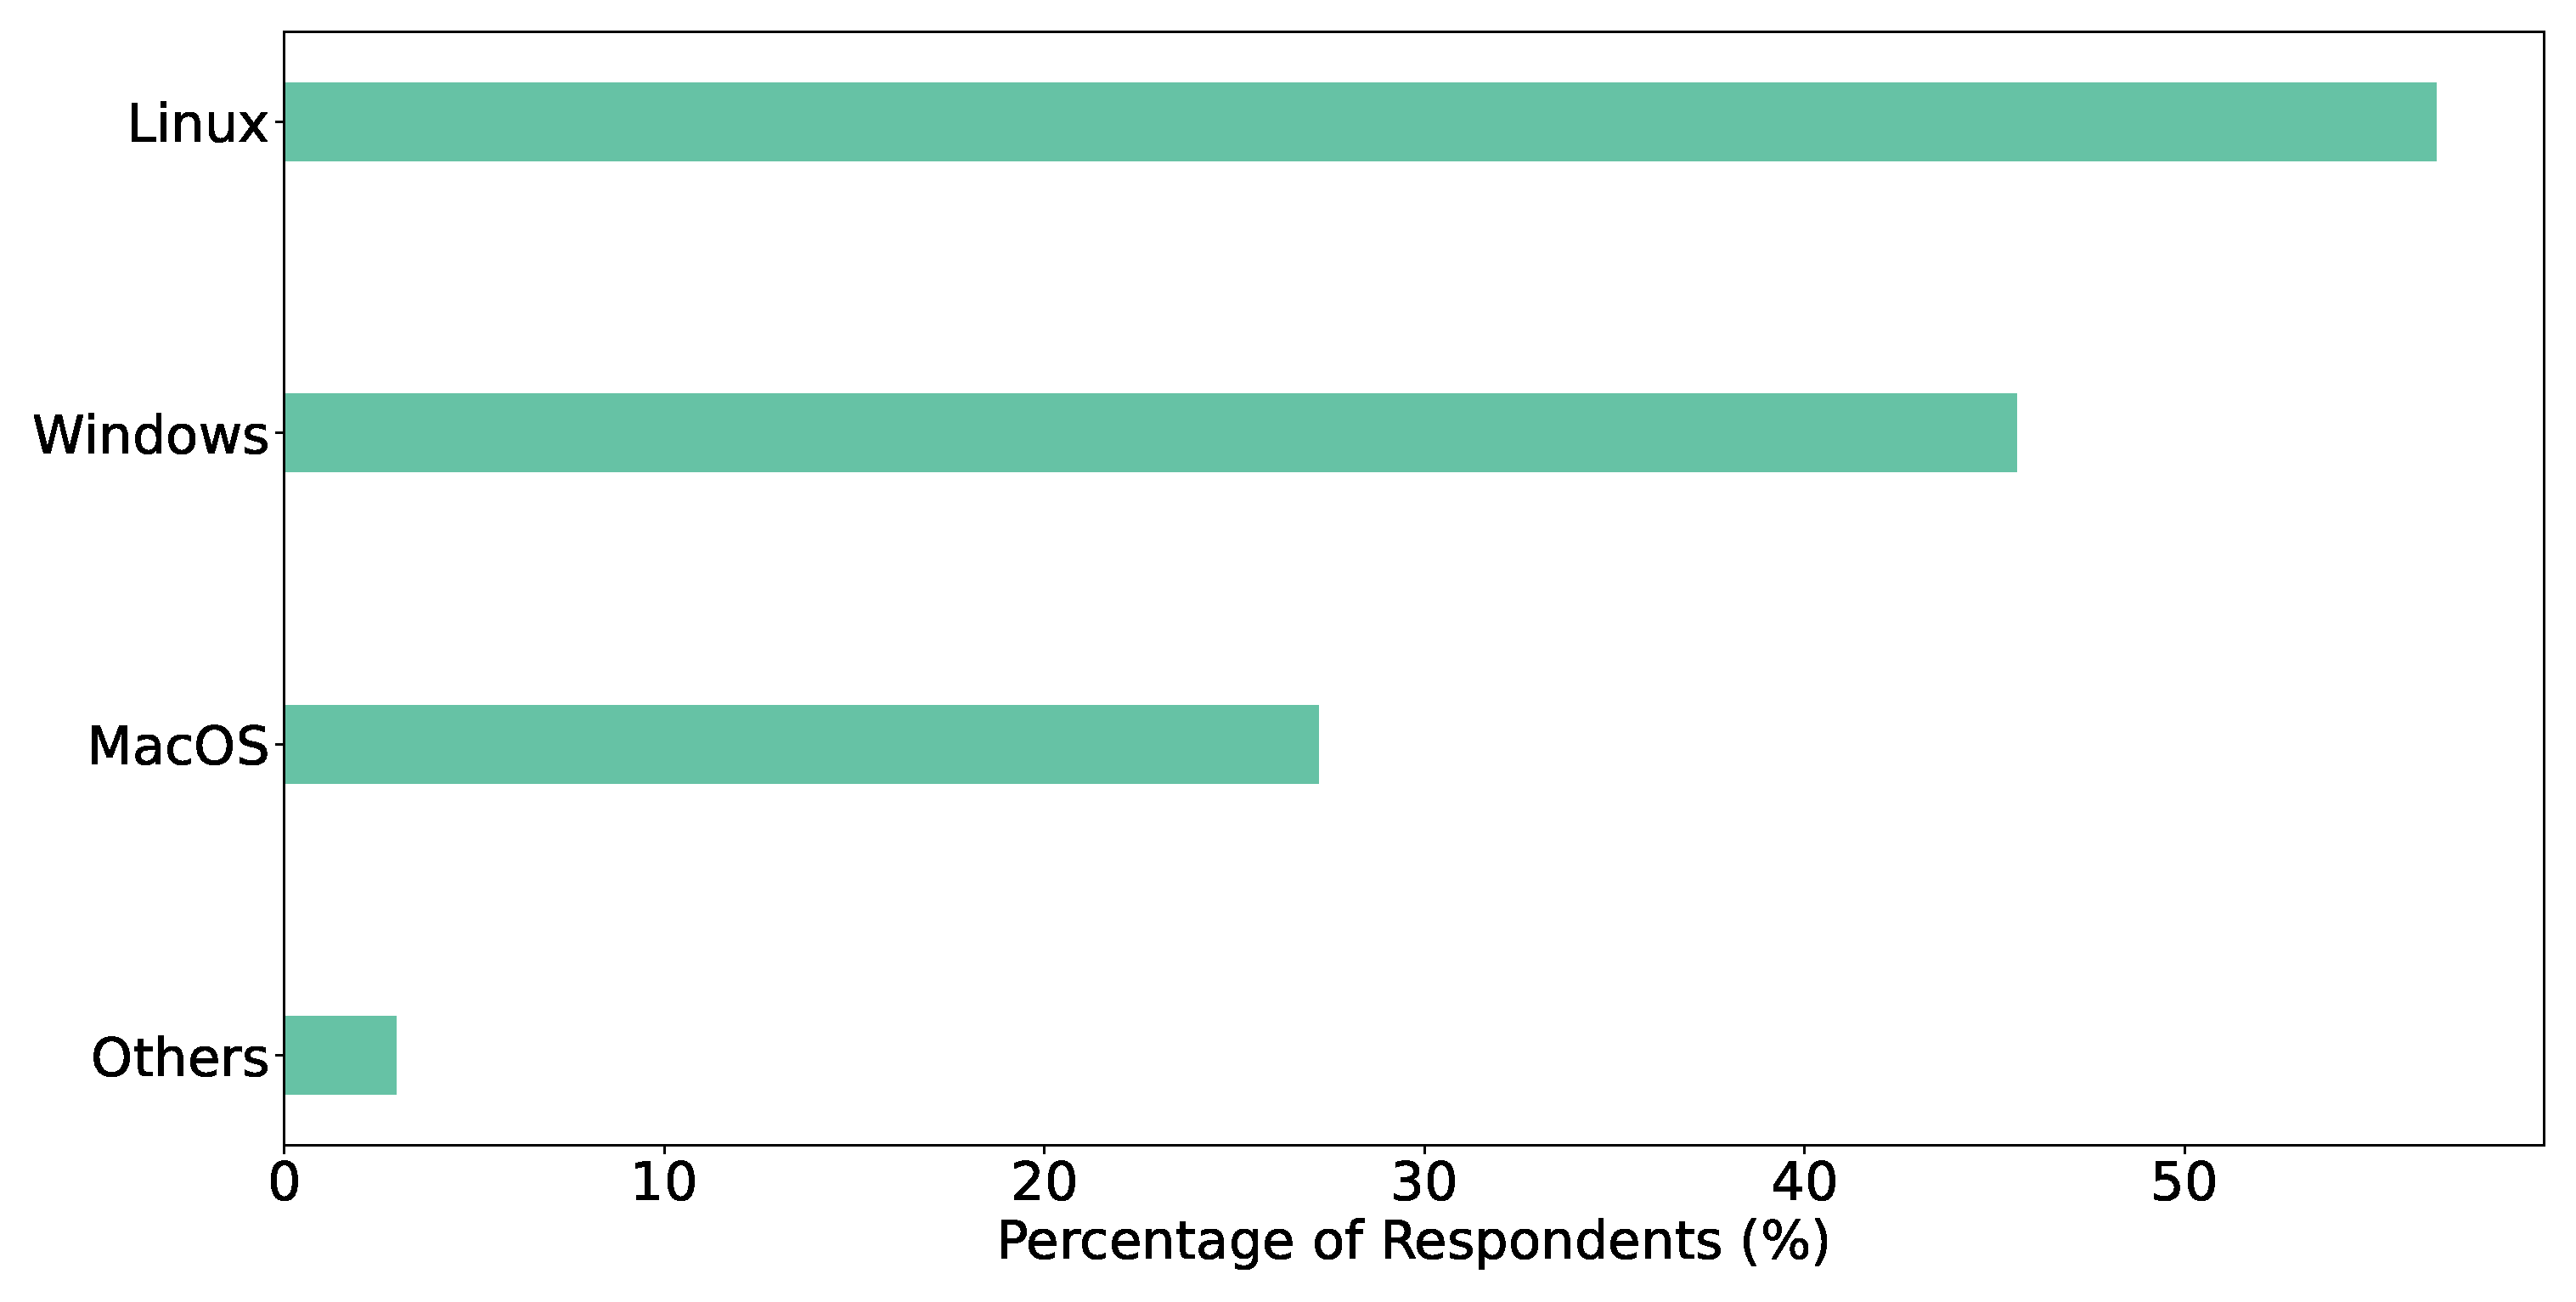
\includegraphics[width=0.8\textwidth]{Figures/Respondents_os}
%   \caption{Operating Systems}
%   \label{fig:os}
% \end{figure}

\paragraph{Programming Languages}
According to \ref{fig:languages}, around 61\% of our respondent's used Java and Javascript each. Other languages like php (25\%), python (25\%), c\# (18\%) are also used which indicates that the software engineers are not inclined towards a single specific language. Also the choice of programming languages used for development can have important inferences for the testing practices of a software company.

% \begin{figure}[htbp]
% \centering
%   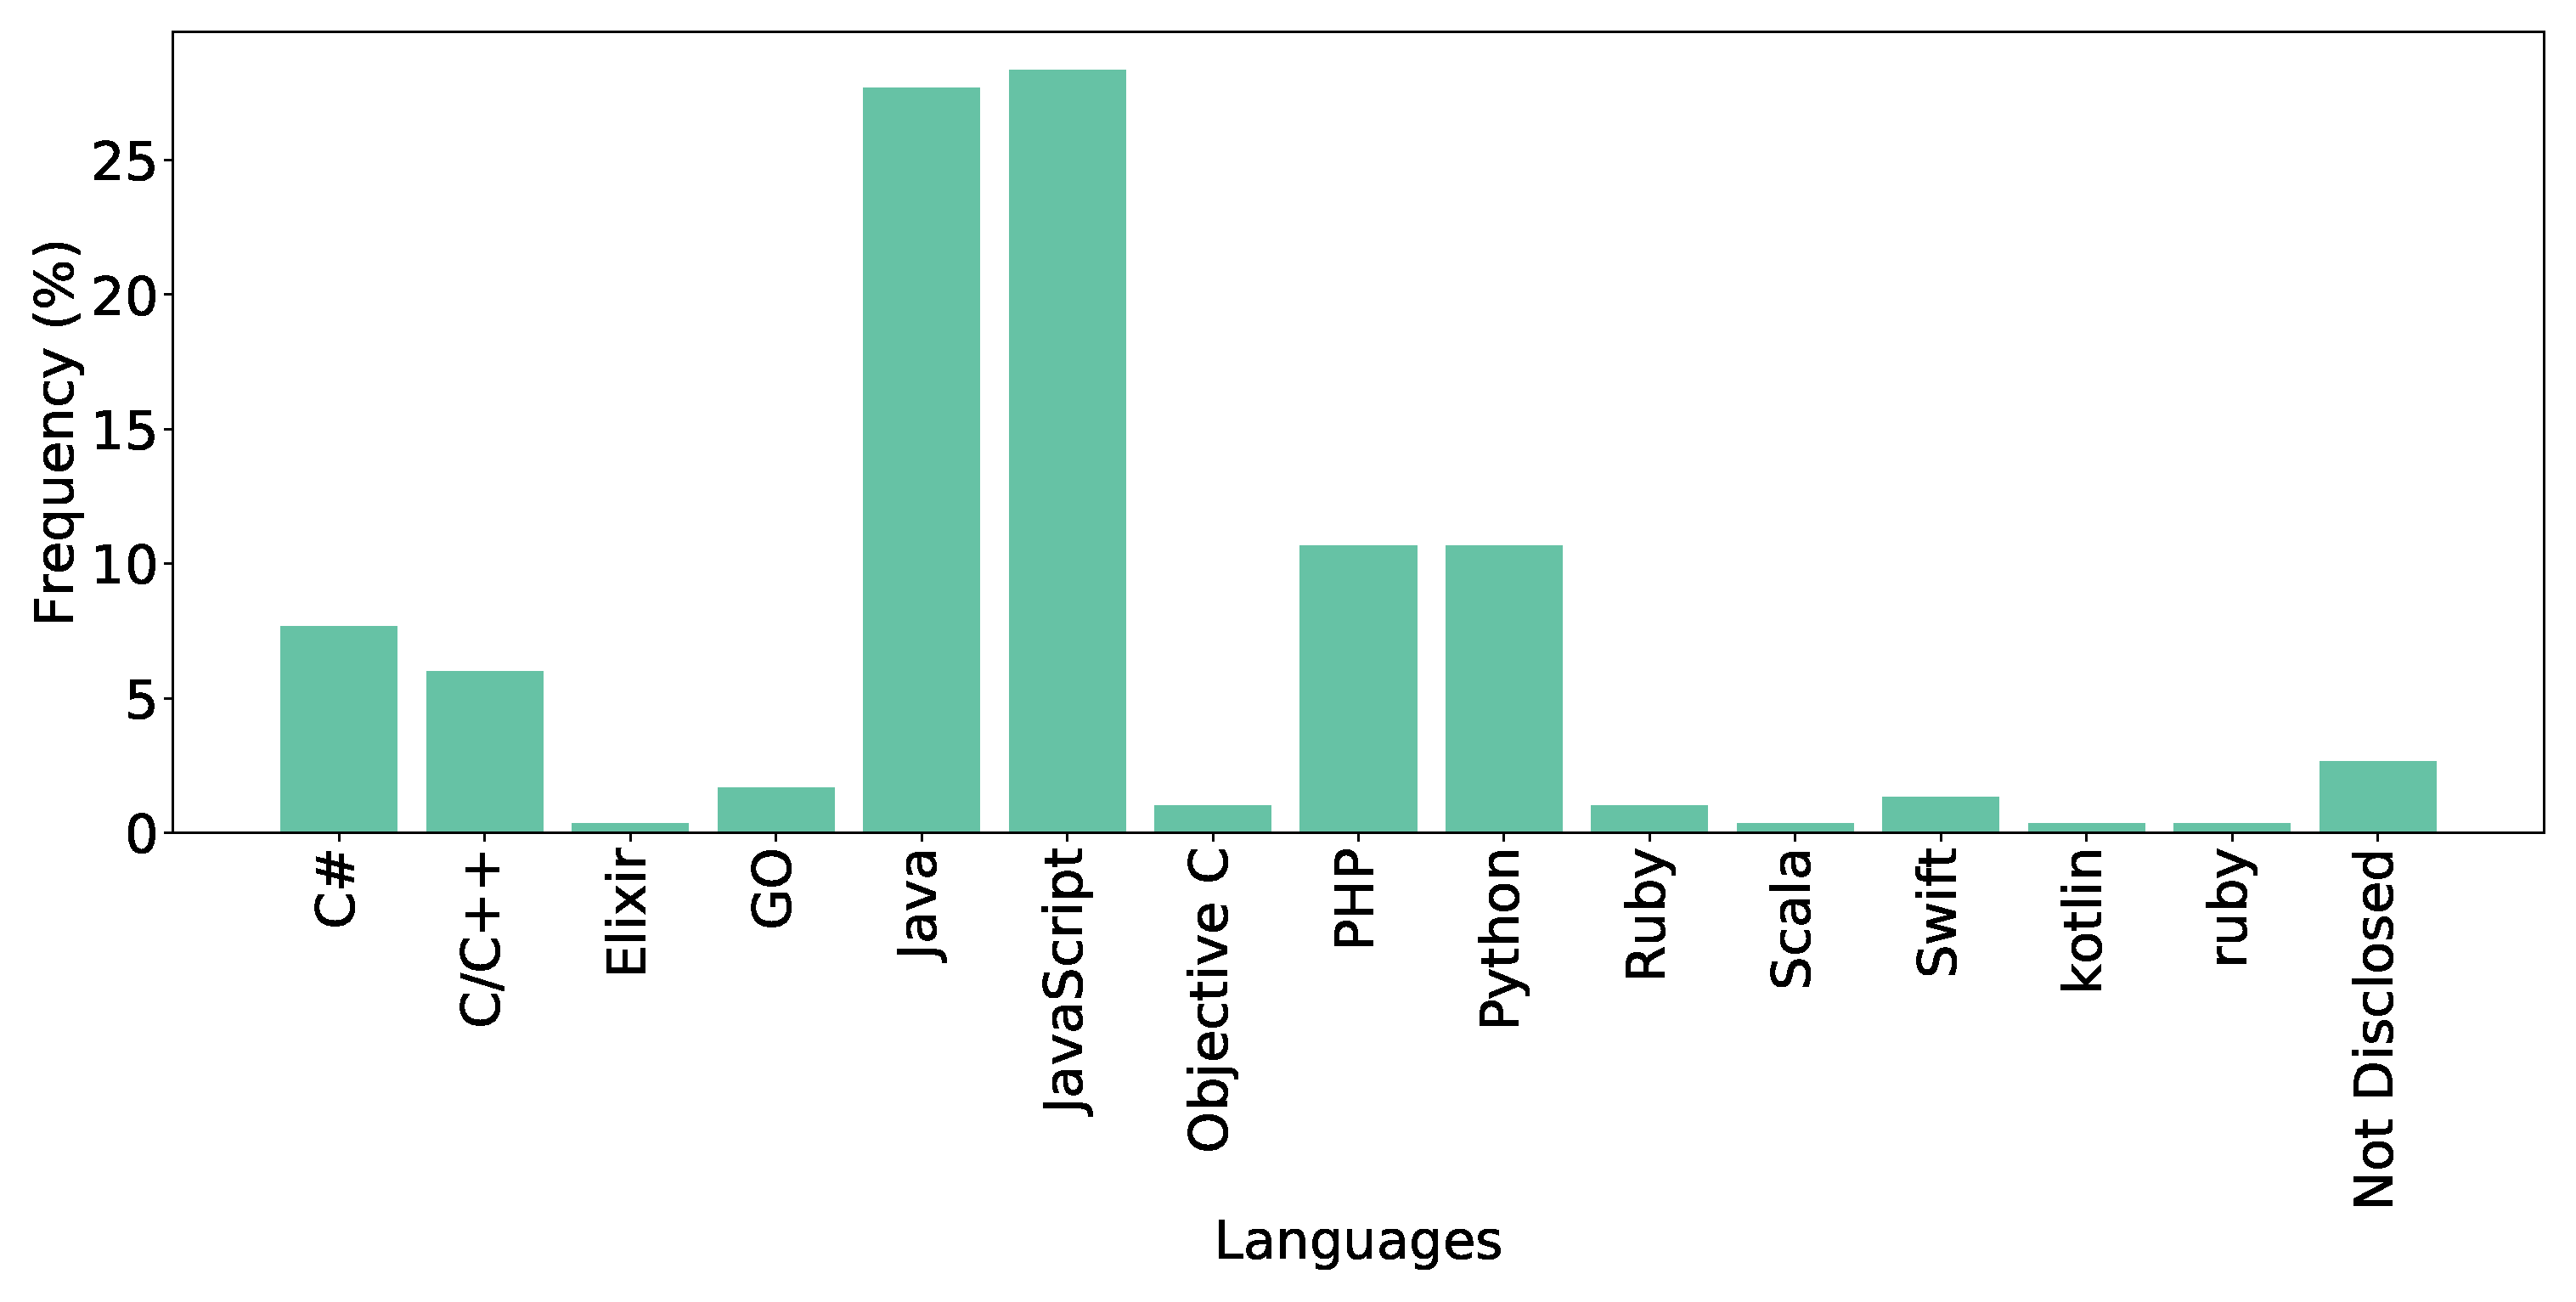
\includegraphics[width=0.8\textwidth]{Figures/Respondents_languages}
%   \caption{Languages used in software development}
%   \label{fig:languages}
% \end{figure}

\paragraph{Frameworks used in development}
As shown in \ref{fig:frameworks}, variety of frameworks have been used during development. Spring boot (37\%) is the mostly used framework in the industry. ASP.NET, Django and Laravel are used in same proportion (14\%).
% \begin{figure}[htbp]
% \centering
%   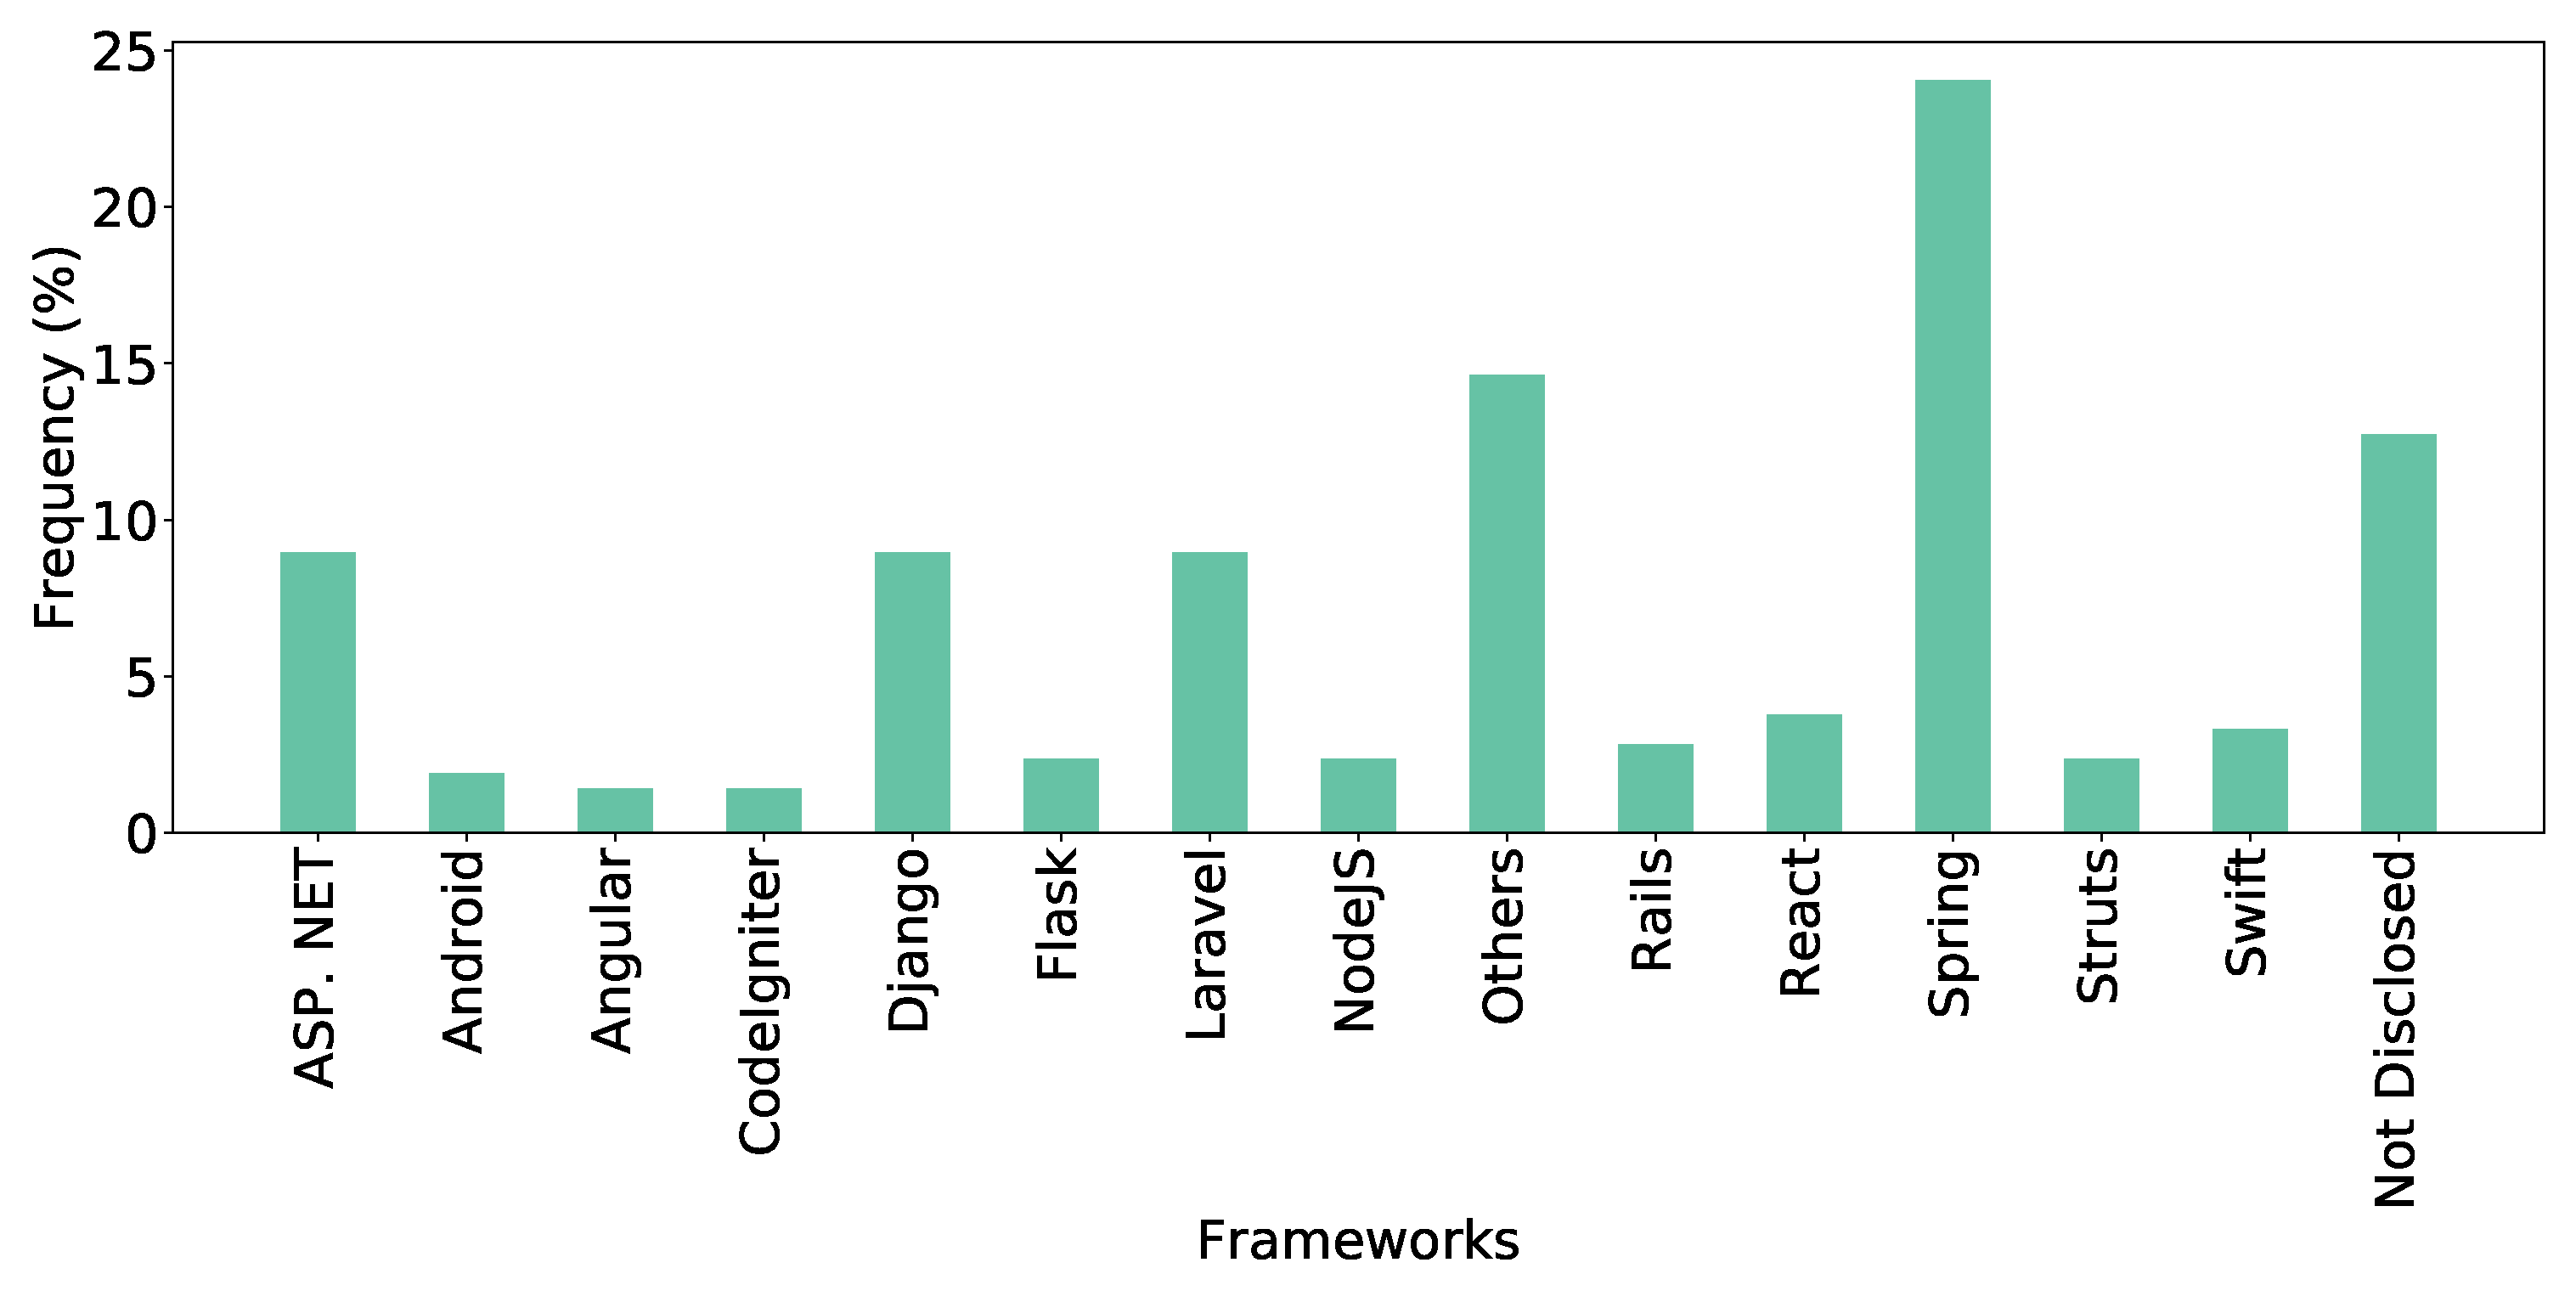
\includegraphics[width=0.8\textwidth]{Figures/Respondents_frameworks}
%   \caption{Frameworks}
%   \label{fig:frameworks}
% \end{figure}

\paragraph{IDE's used by the respondent's}
According to \ref{fig:IDEs}, IntelliJ, a Java integrated development environment for developing computer software for enterprise, mobile, and web development used by most of the respondents (43\%). The other IDEs used in SE industries are: visual studio (30\%), Eclipse (24\%), PyCharm (16\%), NetBeans (10\%), Android Studio (6\%).
% \begin{figure}[htbp]
% \centering
%   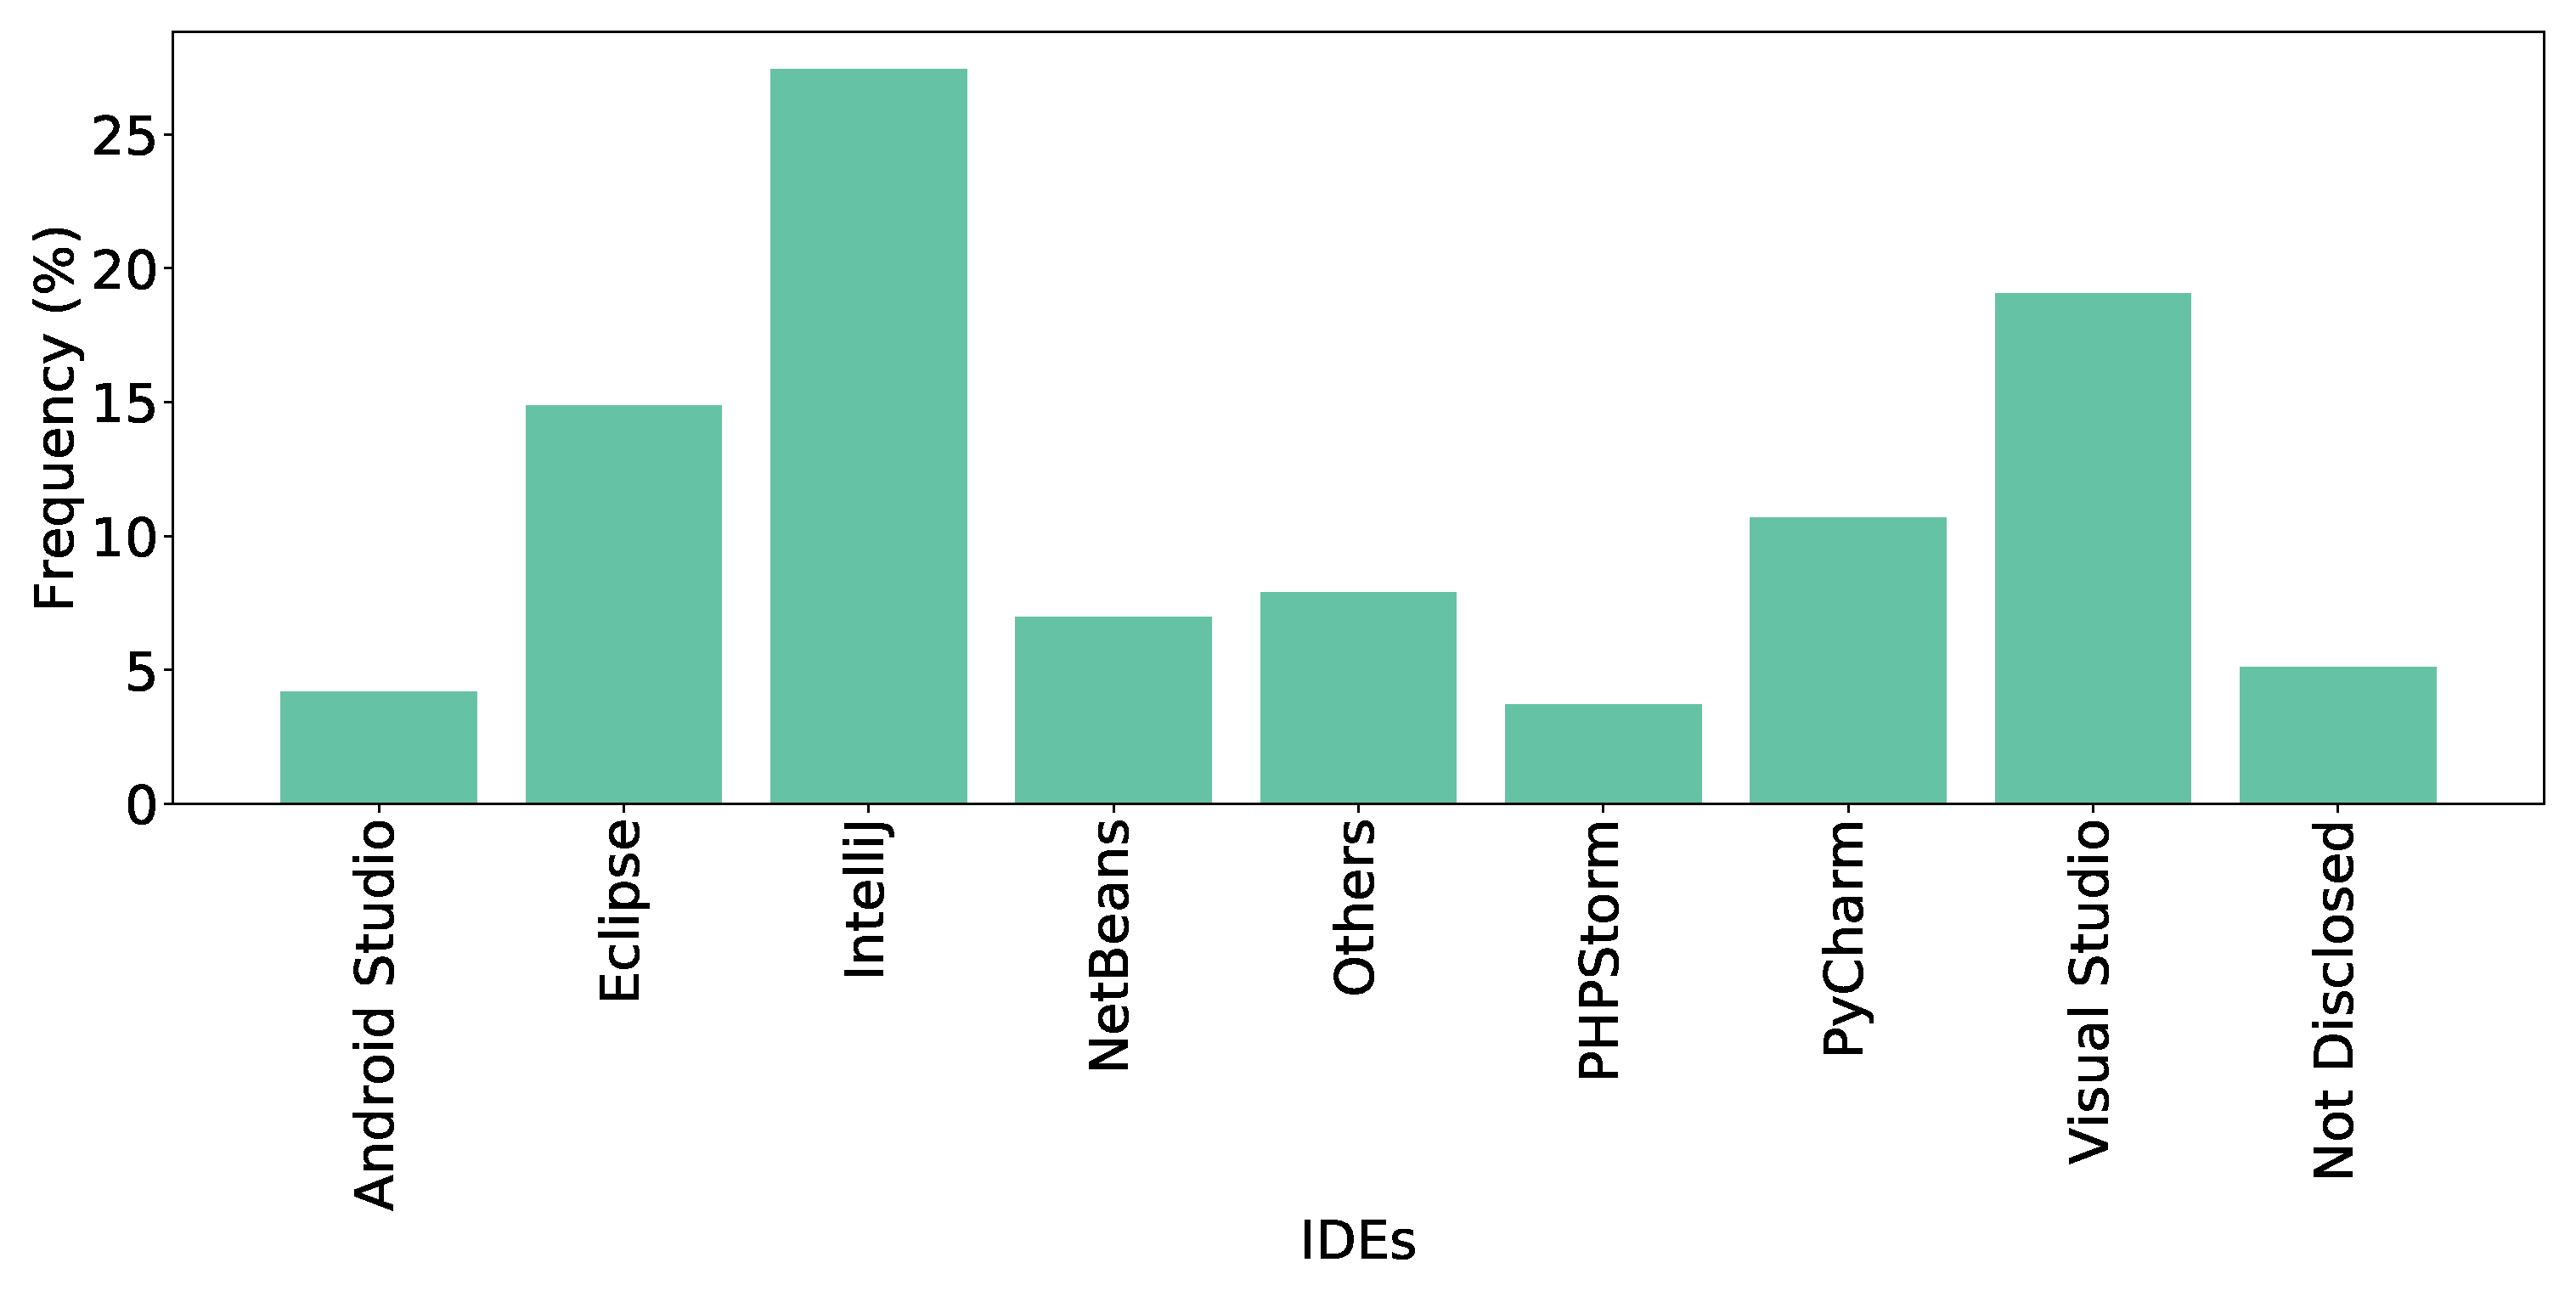
\includegraphics[width=0.8\textwidth]{Figures/Respondents_IDEs}
%   \caption{IDE's}
%   \label{fig:IDEs}
% \end{figure}

\subsubsection{What type of testing and deployment practices are used?}
\label{testing_practices}

Testing is an important process in improving the quality of the software product. The purpose of this process is to find errors, which might occur during specification, design and code generation. Here we report the following results next:
\begin{itemize}
\item Software Testing Practices (Q 14)
\item Level of Automated Testing (Q 15)
\item Tools Used in Testing and QA (Q 16)
\item Continuous Deployment tools (Q 17)
\item Version Control (Q 18)
\end{itemize}


\paragraph{Software Testing Practices}
According to \ref{fig:testing}, several number of testing practices are used during software development. The results show most of the organizations carried out unit testing (53\%), functional testing (49\%), user acceptance testing (39\%), GUI testing (31\%) etc.

% \begin{figure}[htbp]
% \centering
%   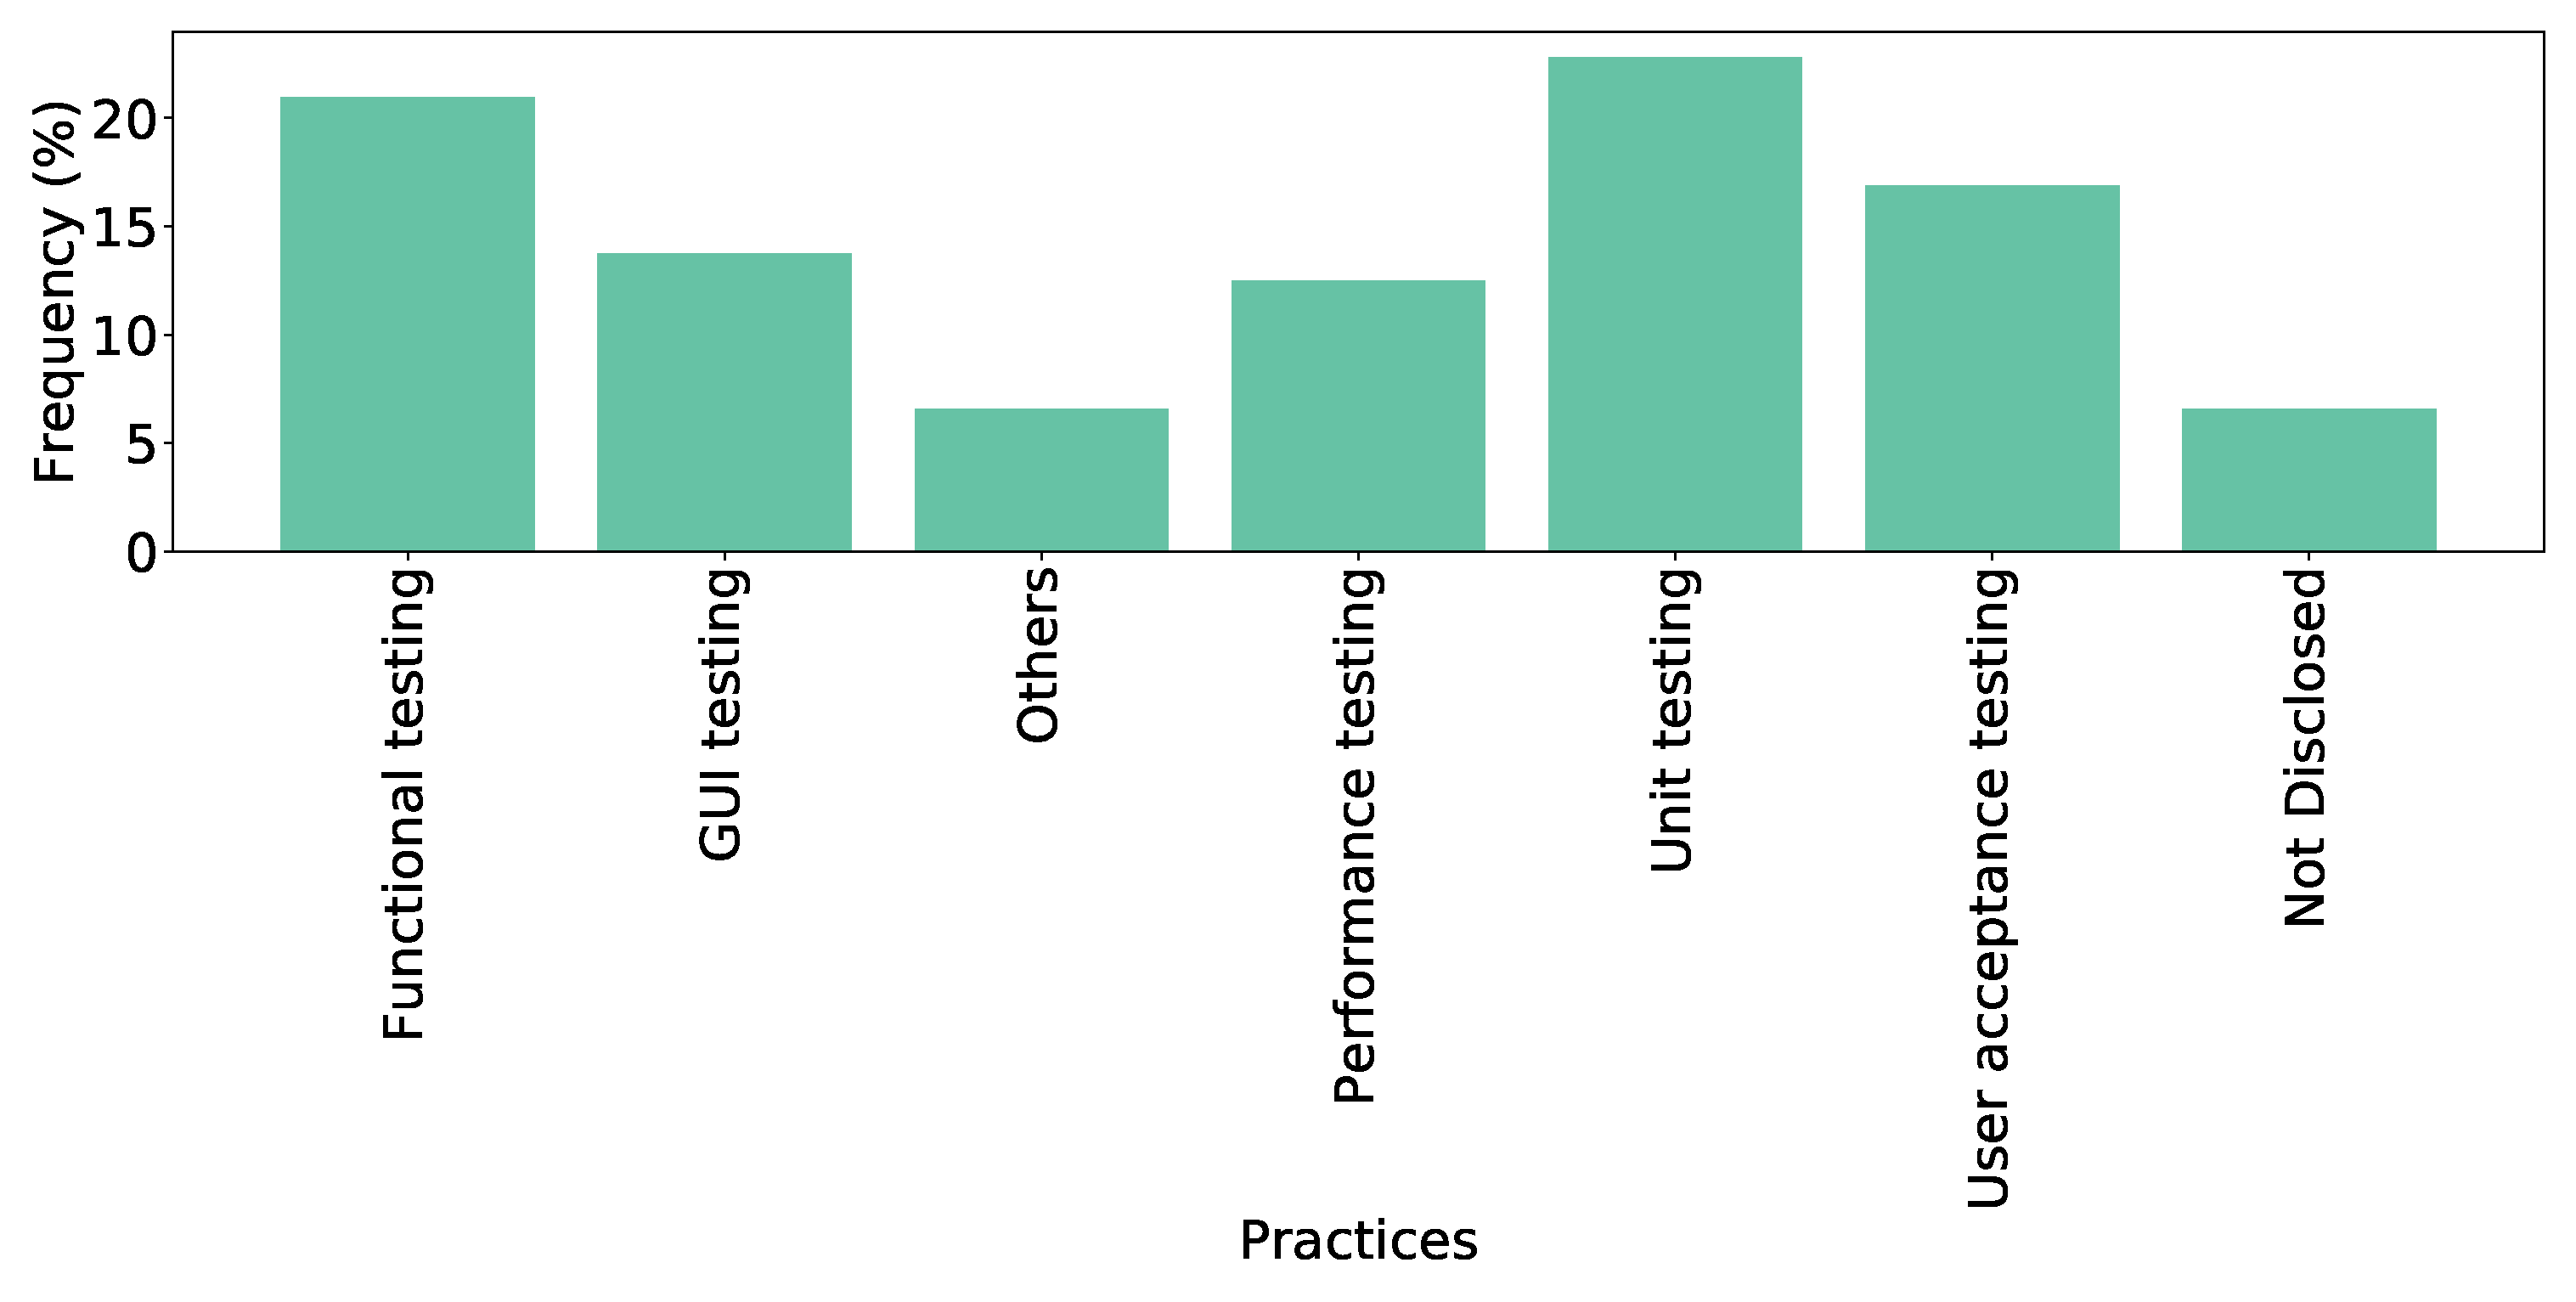
\includegraphics[width=0.8\textwidth]{Figures/Respondents_testing_practices}
%   \caption{Testing Practices}
%   \label{fig:testing}
% \end{figure}


\paragraph{Level of Automated Testing}
Question 15 asked about the level of automated testing. The responses were gathered using the Likert scale. This denotes that different respondents have very different practices in this context, i.e., some heavily practice automated testing, while others favor manual testing. Results are shown in \ref{fig:autoTest}.

% \begin{figure}[htbp]
% \centering
%   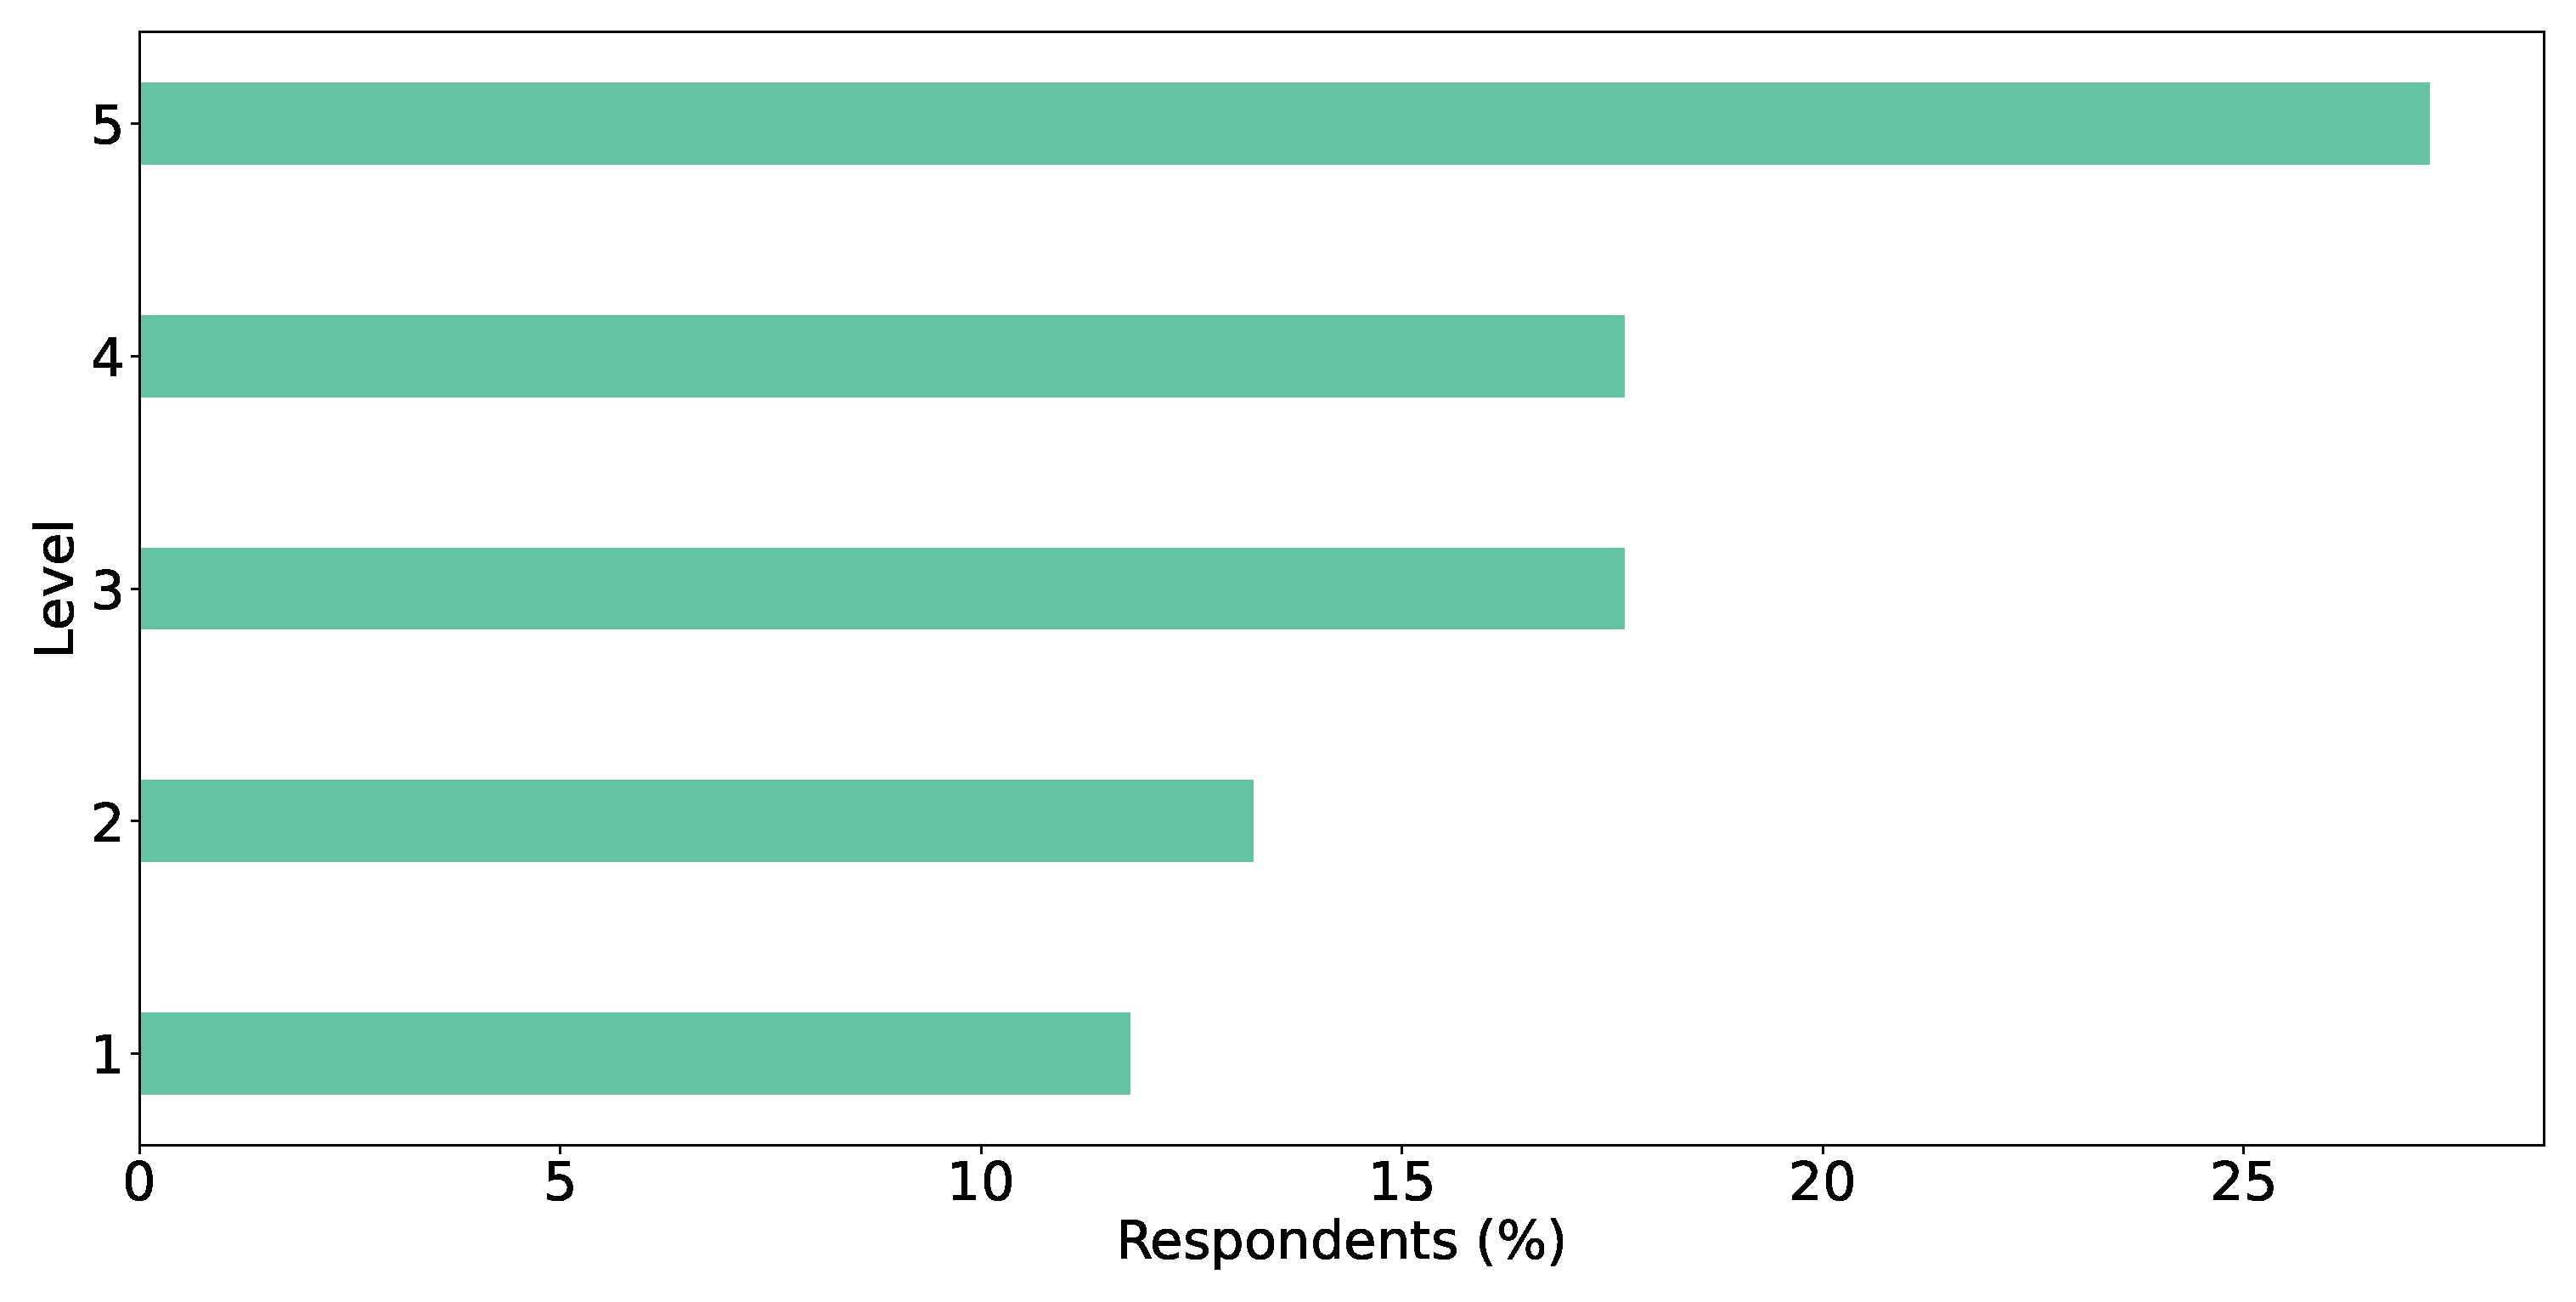
\includegraphics[width=0.8\textwidth]{Figures/Respondents_autotest_level}
%   \caption{Automated Testing Level}
%   \label{fig:autoTest}
% \end{figure}


\paragraph{Tools Used in Testing and QA}
Q 16 asked about the tools used in testing and quality assurance. According to \ref{fig:testingTools}, we see that most of the respondents have been used XUnit( eg, JUnit, NUnit) (30\%), selenium (27\%), Jenkins (20\%), others (9\%).

% \begin{figure}[htbp]
% \centering
%   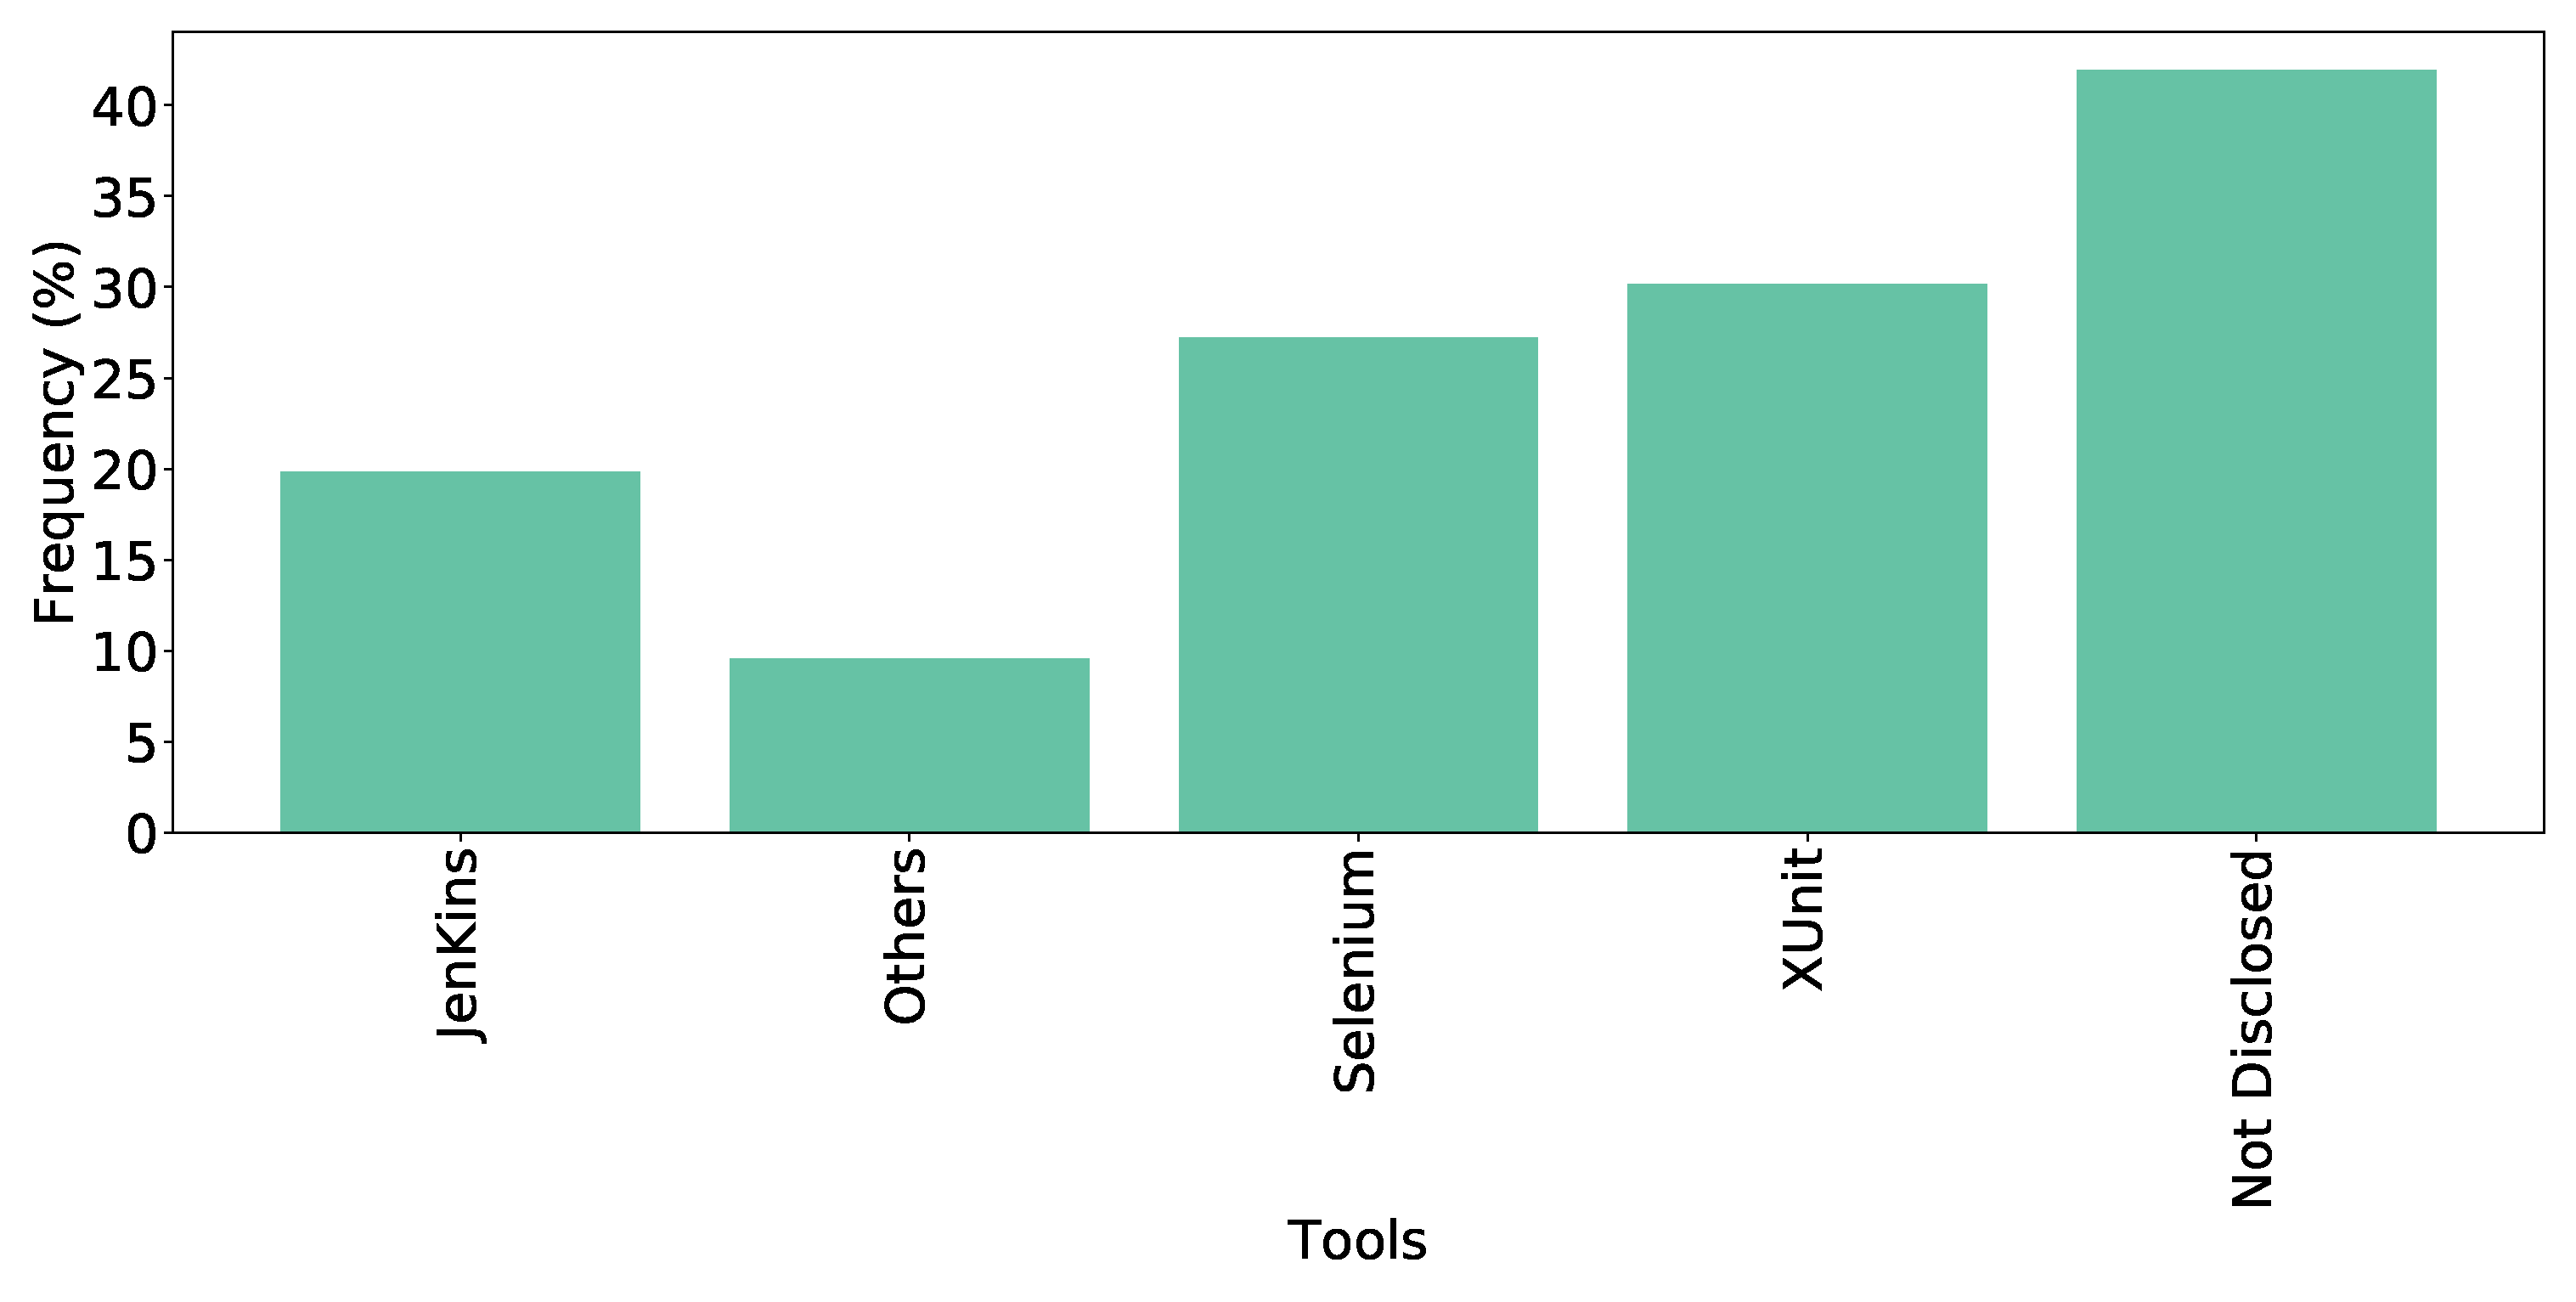
\includegraphics[width=0.8\textwidth]{Figures/Respondents_testing_tools}
%   \caption{Testing \& QA Tools}
%   \label{fig:testingTools}
% \end{figure}


\paragraph{Deployment Tools}
According to \ref{fig:deployTools}, wee see that most of the respondents use AWS code-deploy (12\%) and JenKins (12\%). The other deployment tools are Bamboo (5\%), teamcity (4\%), octopus (2\%). Respondents voted none (4\%) as they didn’t use any deployment tools.

% \begin{figure}[htbp]
% \centering
%   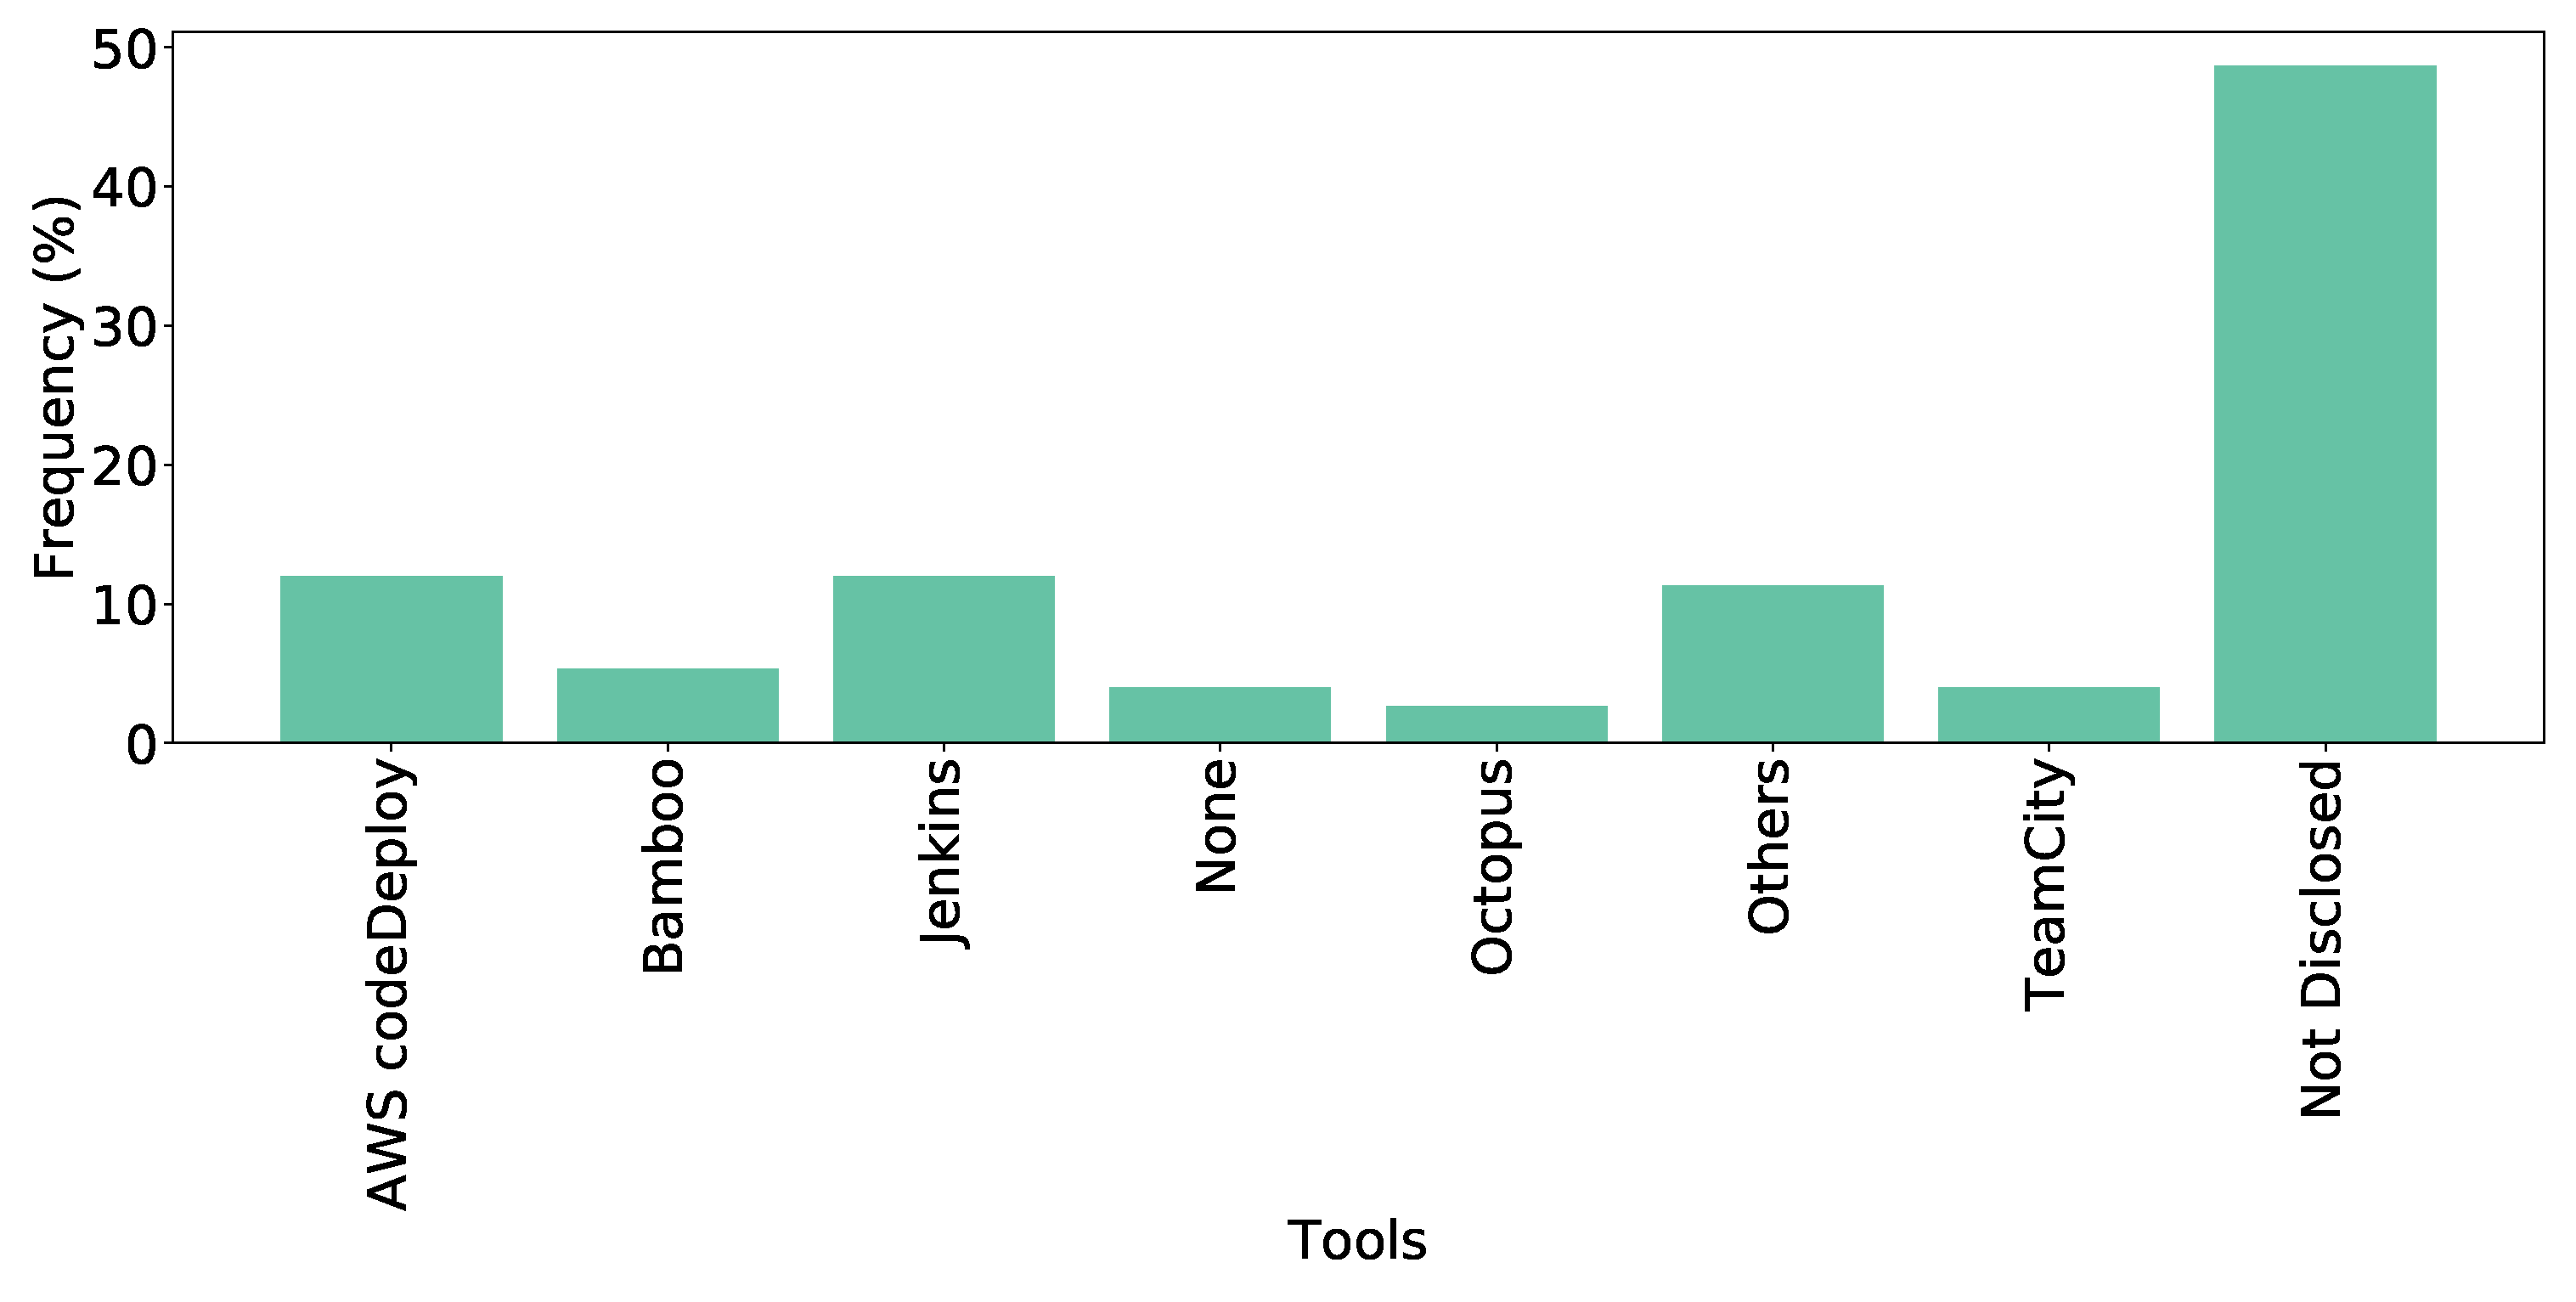
\includegraphics[width=0.8\textwidth]{Figures/Respondents_deployment_tools}
%   \caption{Deployment Tools}
%   \label{fig:deployTools}
% \end{figure}

\paragraph{Version Control}
% \hfill\\
Respondents were allowed to select more than one option. As shown in figure \ref{fig:versionControl}, Git (78\%) and Bit-Bucket (29\%) are mostly-used version control in the software industry. Beside these Subversion (SVN) (5\%), others (4\%) are used.  The 2018 Stack overflow survey\cite{StackoverflowSurvey2018} reports that  the most popular version control system is Git (87.2\% developer uses Git) and the second most popular is SVN (16.1\% developer uses SVN). However, in our survey, we found slightly different result,the most popular version control system is Git and the second most popular is Bit-bucket. This might be related  to the declining popularity of SVN over the years. From the Stack overflow survey over the range 2017-2019, it is clear that SVN is losing popularity to Git. Nowadays, SVN is mainly used for versioning legacy projects. As the SE industry of Bangladesh is quite new, we observe such discrepancy in the popularity of SVN.

% \begin{figure}[htbp]
% \centering
%   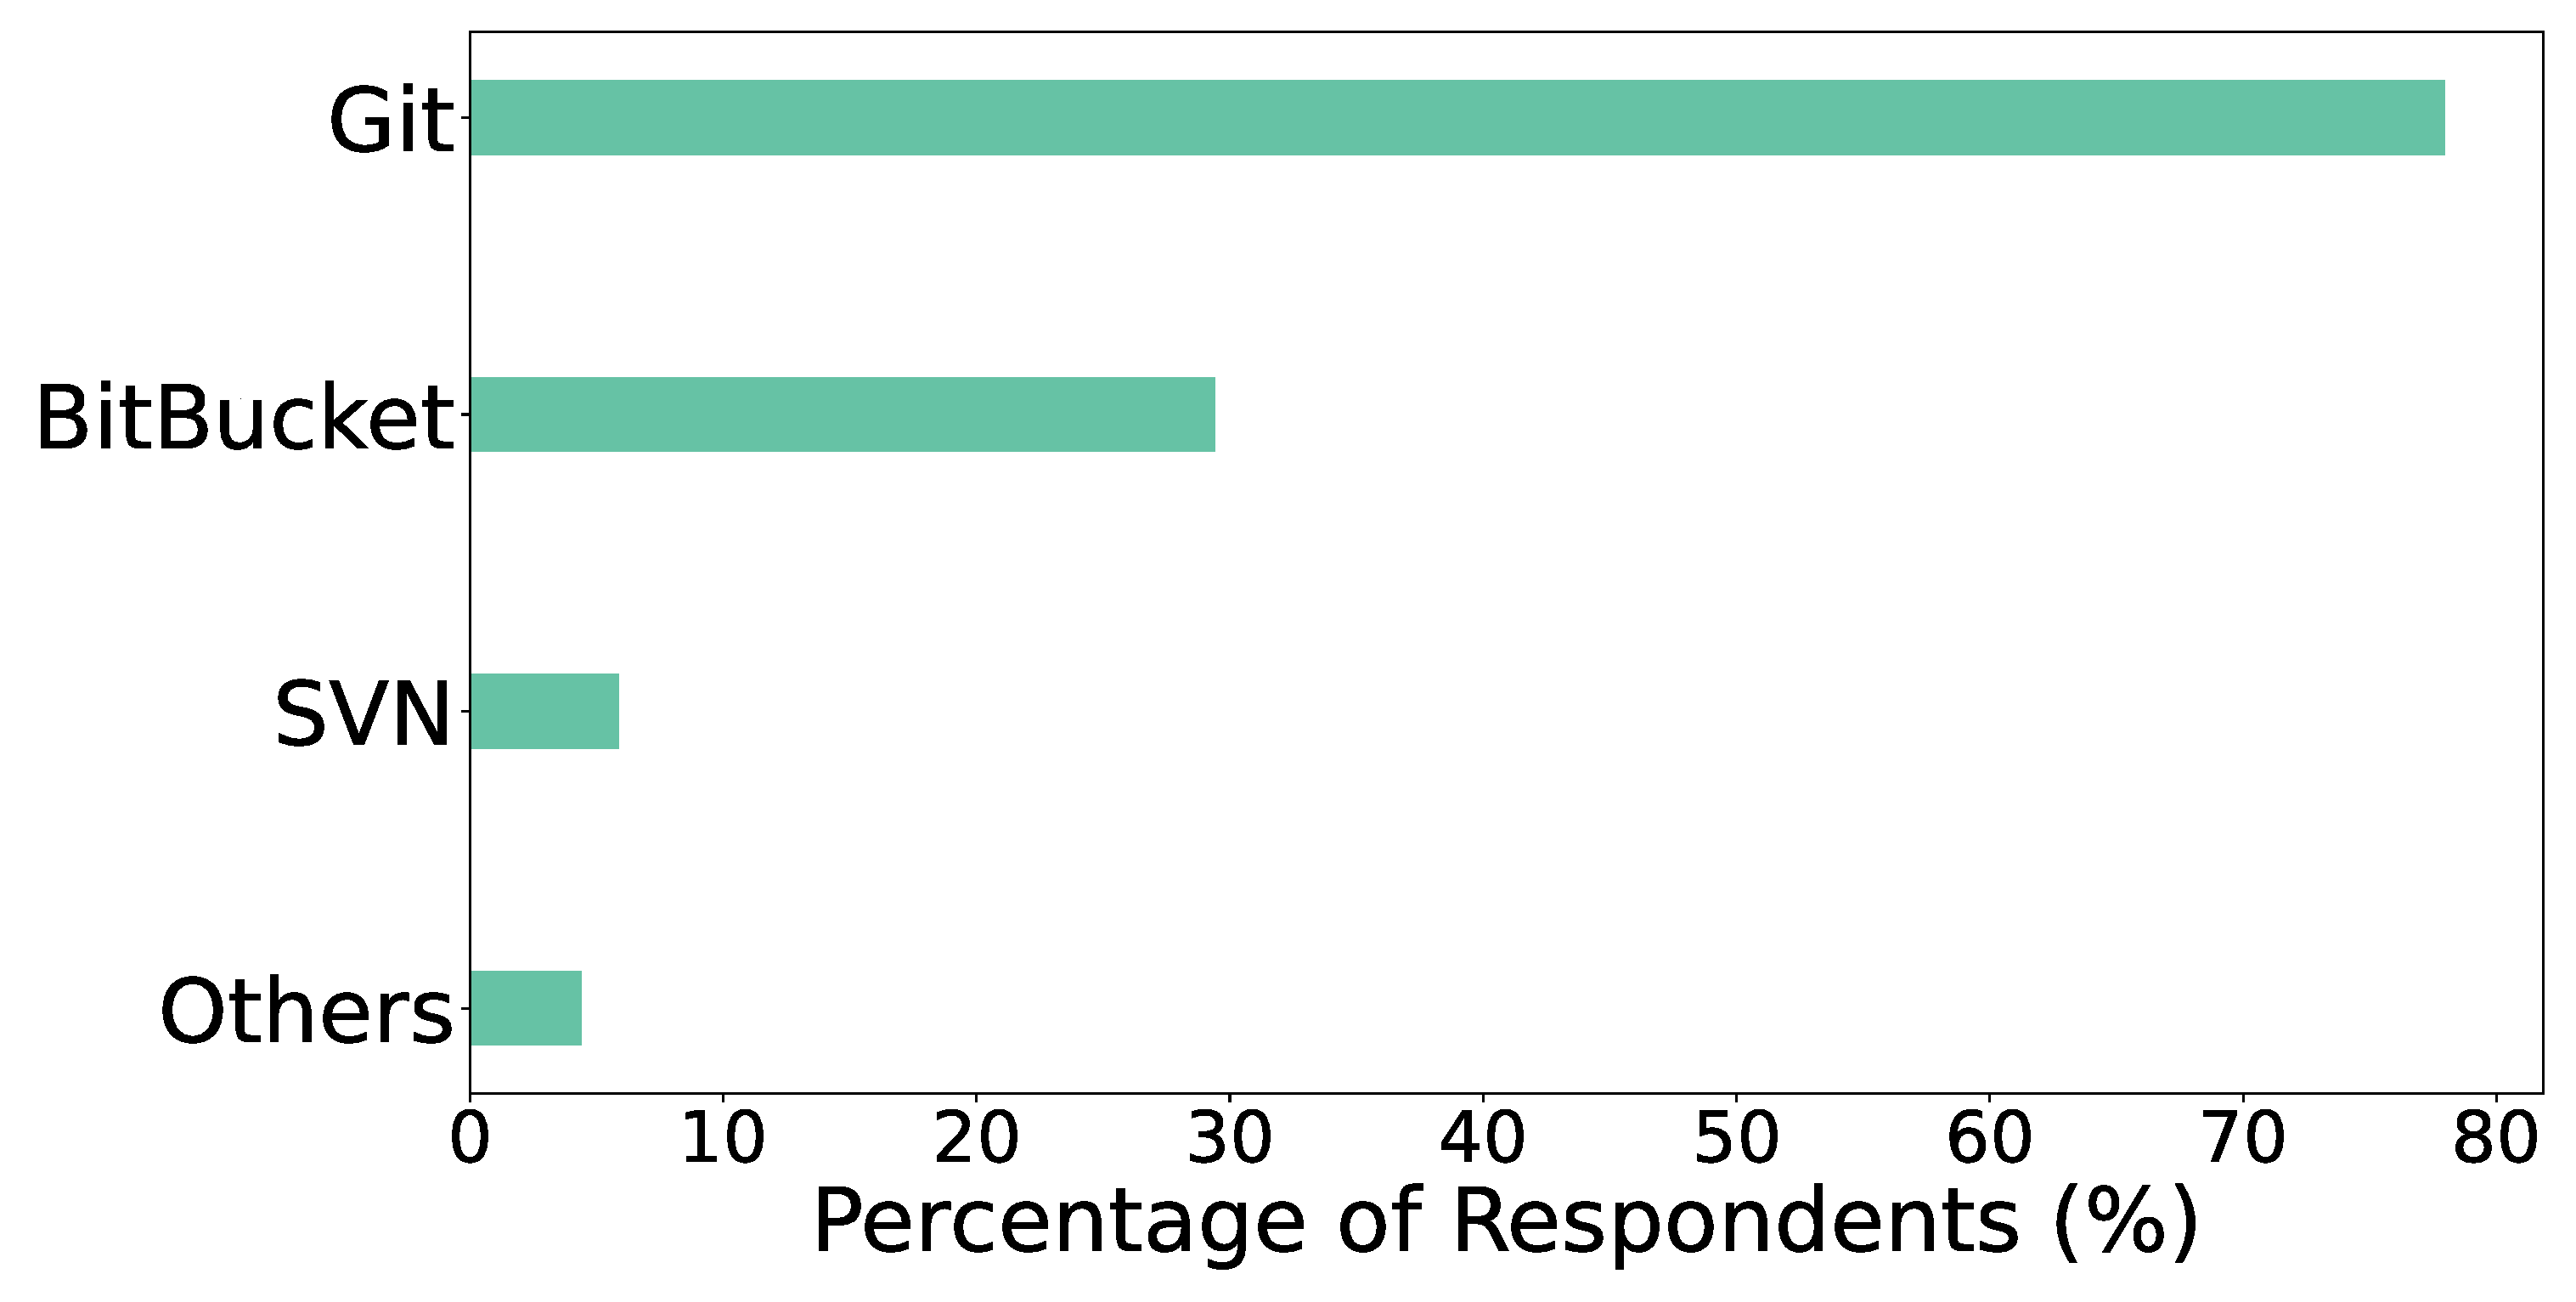
\includegraphics[width=0.8\textwidth]{Figures/Respondents_version_control}
%   \caption{Version Control}
%   \label{fig:versionControl}
% \end{figure}
\subsubsection{How are the security and performance is ensured in a product of a company?}
\label{security_performance}

To identify general practices among the Bangladesh software industry regarding software products' security and performance, we have included two open-ended questions in the survey. This particular question covers how a company secures its code from external attack and maintain its performance after deployment. However, the performance of a software product is related to the scalability of the solution. So, we will cover the following points here:
\begin{itemize}
    \item Security
    \item Performance
    \item Scalability
\end{itemize}


\paragraph{Security:}
\label{Security}
% \begin{figure}[htbp]
% 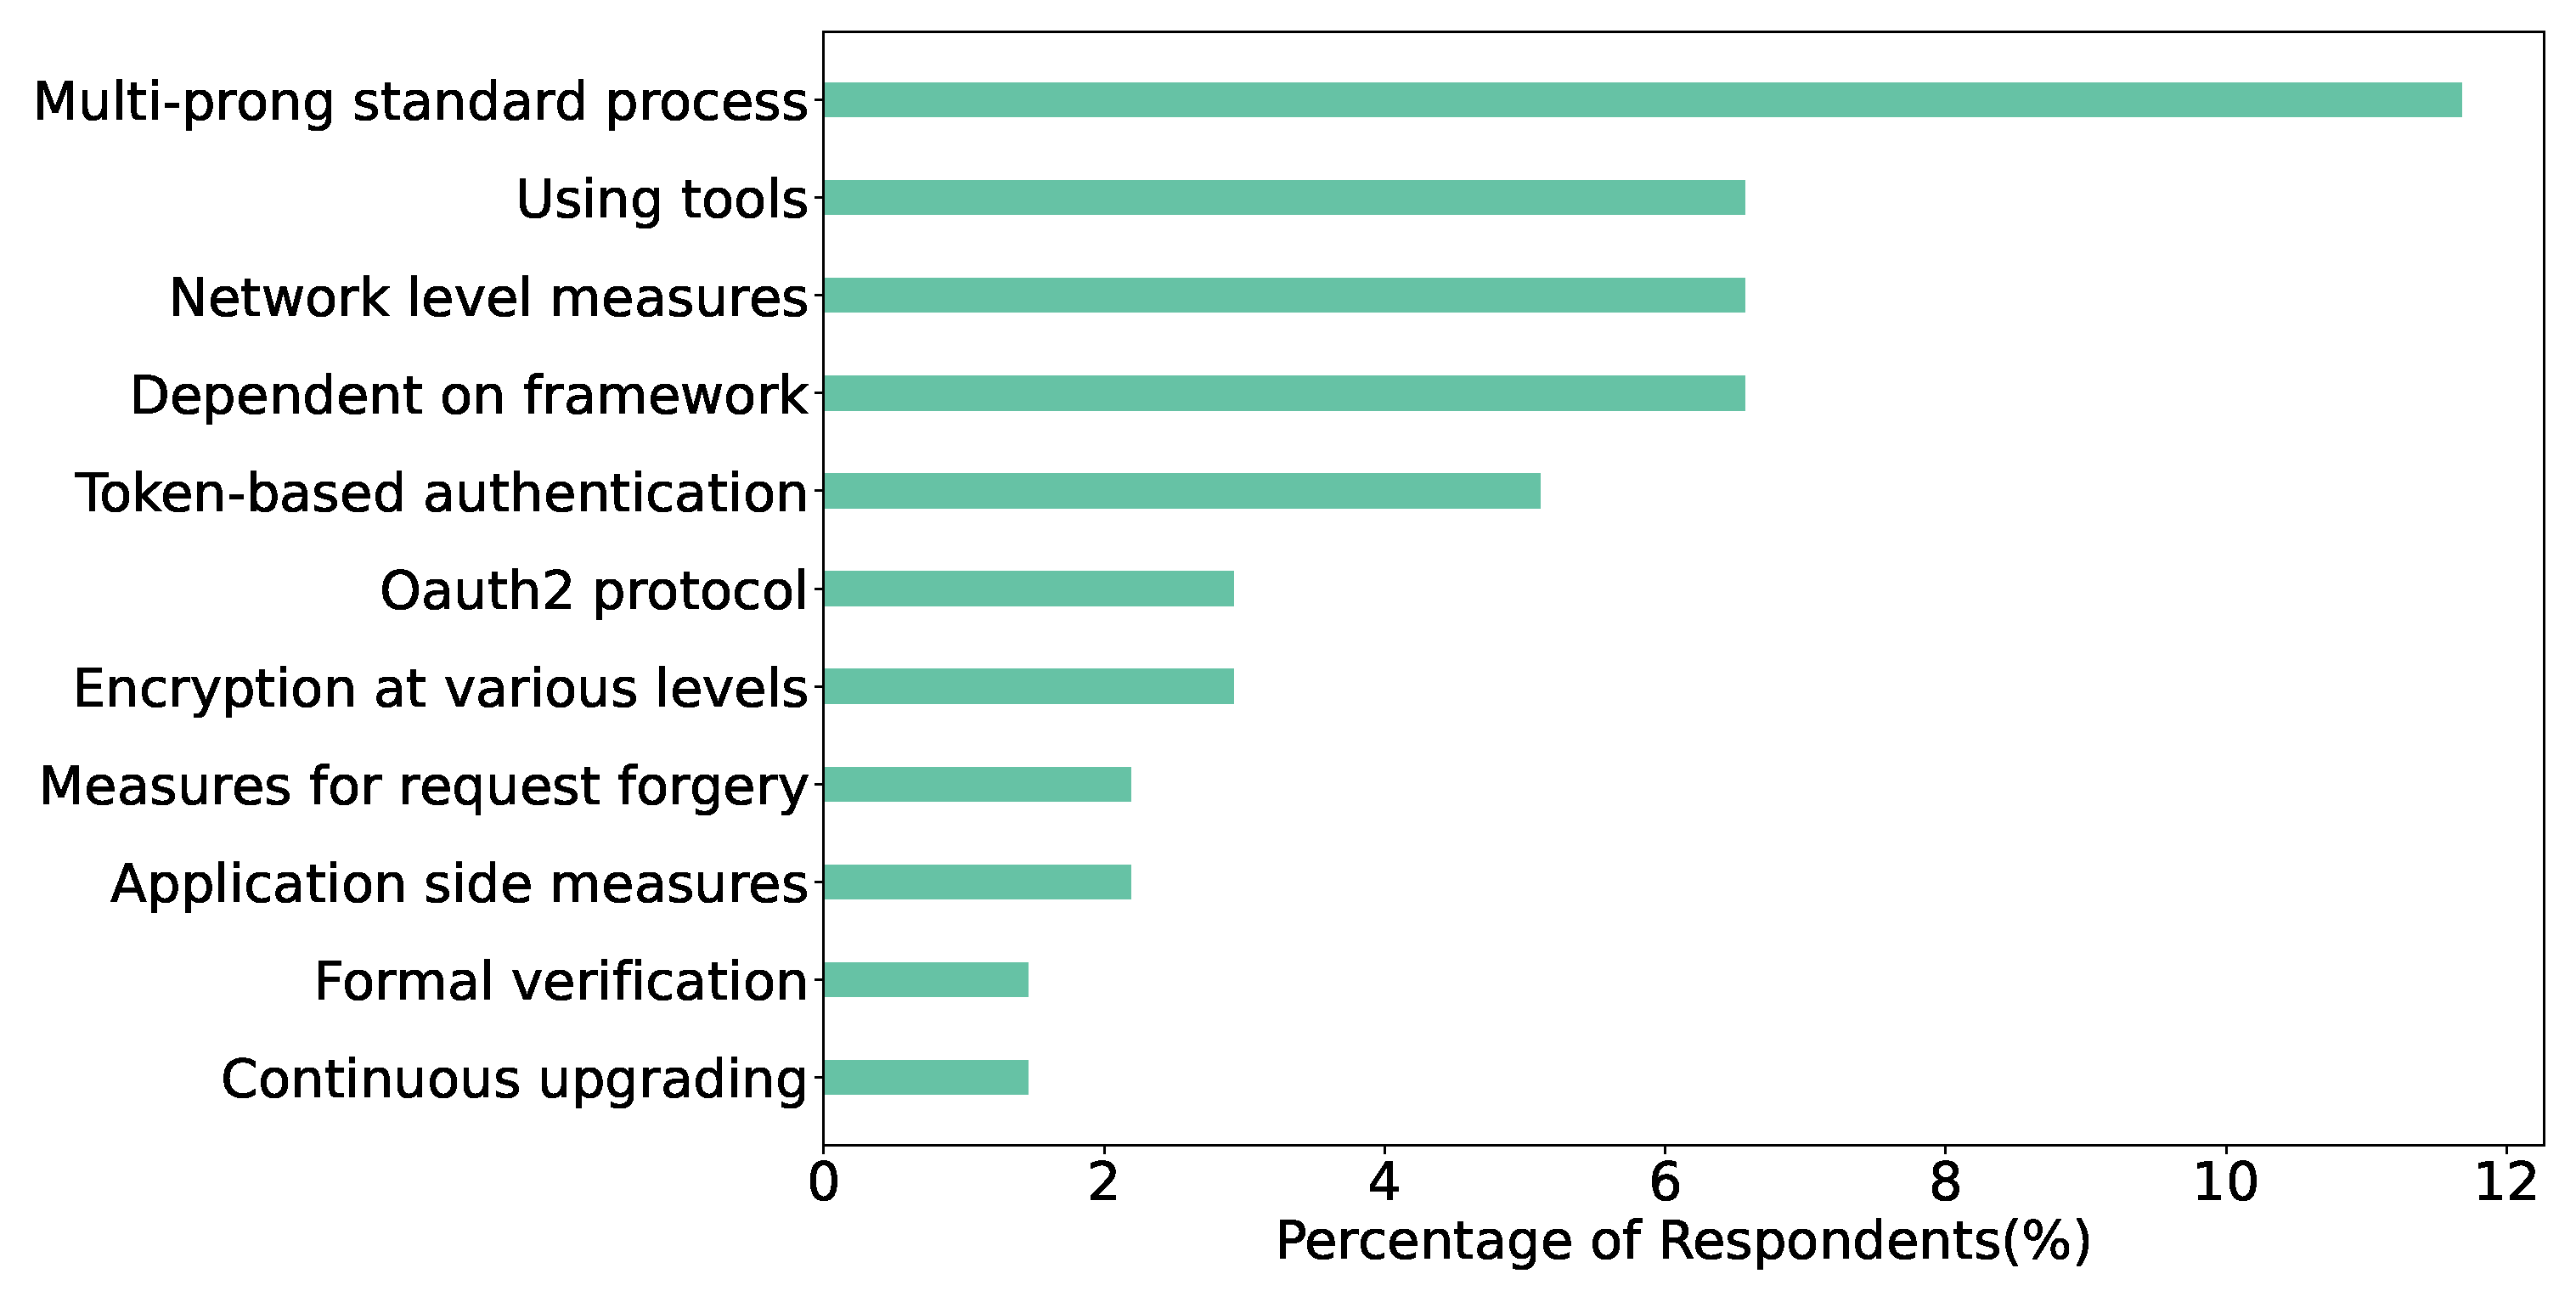
\includegraphics[scale=0.28]{Figures/Security.eps} 
% \caption{Measures to maintain security of products}
% \label{fig:Measures to ensure security}
% \end{figure}
% \hfill\\

Authentication and authorization-based security are the most prominent practice in the Bangladesh software industry to ensure software products' security. The other categories are security based on framework/platform/tools and encryption. Under these categories, several measures are usually followed. The measures of the security categories are discussed below,
Measures under the \emph{authentication and authorization} category is practised by 25.5\% respondents to ensure security. The measures are 
\begin{enumerate}[label=(\alph*)]

    \item \textbf{Multi-prong Standard Process} : About 10.22\% of the total respondents reported that they practices various security standard and protocol to ensure security. The standard includes ISO/IEC 27001 , and PA DSS
    \surveyquote{Multi Prong Standard Processes and Products}{110}
    
    \item \textbf{Token-based authentication} : A token-based authentication system allows users to enter their username and password to obtain a token, which allows them to fetch a specific resource - without using their username and password. Once their token has been obtained, the user can offer the token, which offers access to a specific resource for a time period - to the remote site. 5.11\% of people expressed its eligibility.
    \surveyquote{Token based authentication for all of my rest service}{80}
    
    \item \textbf{OAuth 2.0} : OAuth 2.0 is the industry-standard protocol for authorization. OAuth 2.0 focuses on client developer simplicity while providing specific authorization flows for web applications, desktop applications, mobile phones, and living room devices. Many (2.92\%) respondents use the OAuth 2.0 protocol as the main way of maintaining security.
    \surveyquote{OAuth 2.0, JWT, Token Base Authentication, CORS Filter, XSRF}{127}
    
    \item \textbf{Application Side Measures}: 2.19\% of respondents responded that they implement security measures at the application level. This measure includes encryption of application data at the client-side, use of https while pulling data from a server, secured architecture etc.
    \surveyquote{At application level, could not achieve others yet}{72}
    
    \item \textbf{Measures for request forgery}: Measures against cross-site forgery are implemented to ensure security. This includes CORS or cross-origin resource sharing, CSRF, or cross-site request forgery or one-click attack or XSRF. 2.19\% of respondents implemented measures against  Cross-site request forgery to ensure security.
    \surveyquote{Security testings like: SQL injection, cross-site scripting, CSRF, API security, use of https,  detecting malicious / suspicious HTTP requests and auto-blocking}{42}
    
    \item \textbf{Formal Verification}: A code-level review can mitigate security threats. 1.46\% respondents ensured the practice of formal code review.
    \surveyquote{There are some basic guidelines that we must follow and while code review this needs to be an absolute part that needs to be checked before the code gets merged}{112}
    
\end{enumerate}

21.17\% respondents use several technology, tools,platform to ensure security of their product. Measures under the \emph{framework/platform/tools} category are,
\begin{enumerate}[label=(\alph*)]

     \item \textbf{Dependent on Framework} : The common frameworks provide basic to intermediate level security measures in the application. 6.57\% of respondents depend on the framework for security. The framework includes popular frameworks such as spring and  HDIV.
    \surveyquote{https, popular framework which already prevents some type of attacks. rest of the things on case-by-case basis)}{79}
    
    \item \textbf{Use of tools} : Respondents use various open-source/ paid tools for scanning and testing. These tools help to find security threats in an existing system. The tools include OWASP based tools and  penetration testing tools.
    \surveyquote{use encryption at different level of software (server, network, transmission layer, database and software layer.)}{35}
    
    \item \textbf{Network level Measures}: Network-level measures include IP-white-listing, port-blocking, VPN, and use of HTTPS  in software. 6.57\% of respondents use at least one of the before-mentioned strategies to ensure security.
    \surveyquote{network blocking and common security measures}{2}

    \item \textbf{Continuous Upgrading}: As security threats are evolving; thus, current systems need continuous up-gradation in a frequent interval. 1.46\% of respondents said they arrange frequent hackathons, workshops, and security audits to address the continuously evolving security threat.
    \surveyquote{We run security audit of our office environment. We also conduct security session per 6 months to introduce latest trend in threats and what we can do to avoid it}{57}

\end{enumerate}

2.92\% of respondents use encryption technologies to encrypt their data. Respondents use encryption at the different levels of software architecture such as network, data, transmission, and ensure their security.
\surveyquote{use encryption at different level of software (server, network, transmission layer, database and software layer.)}{35}

% To maintain security of software product SE industry of Bangladesh is mainly dependent on standard process which includes cloud based security, third party software, OS hardening followed by uses of security tools, network level measures and framework security. As found by Harrison et al.\cite{Harrison2010} network level measures are the first choice in ensuring security of software product which matches with our findings. Srinivasan et al.\cite{Srinivasan2017} listed top 10 web framework in terms of security testing where Spring framework achieved 7\textsuperscript{th} position. From figure ~\ref{fig:frameworks} we have seen that most of our respondents use Spring framework for software development. This might be the reason that a lot number of respondents dependent on framework for ensuring security.


\paragraph{Performance}
\label{Performance}

% \begin{figure}[htbp]
% 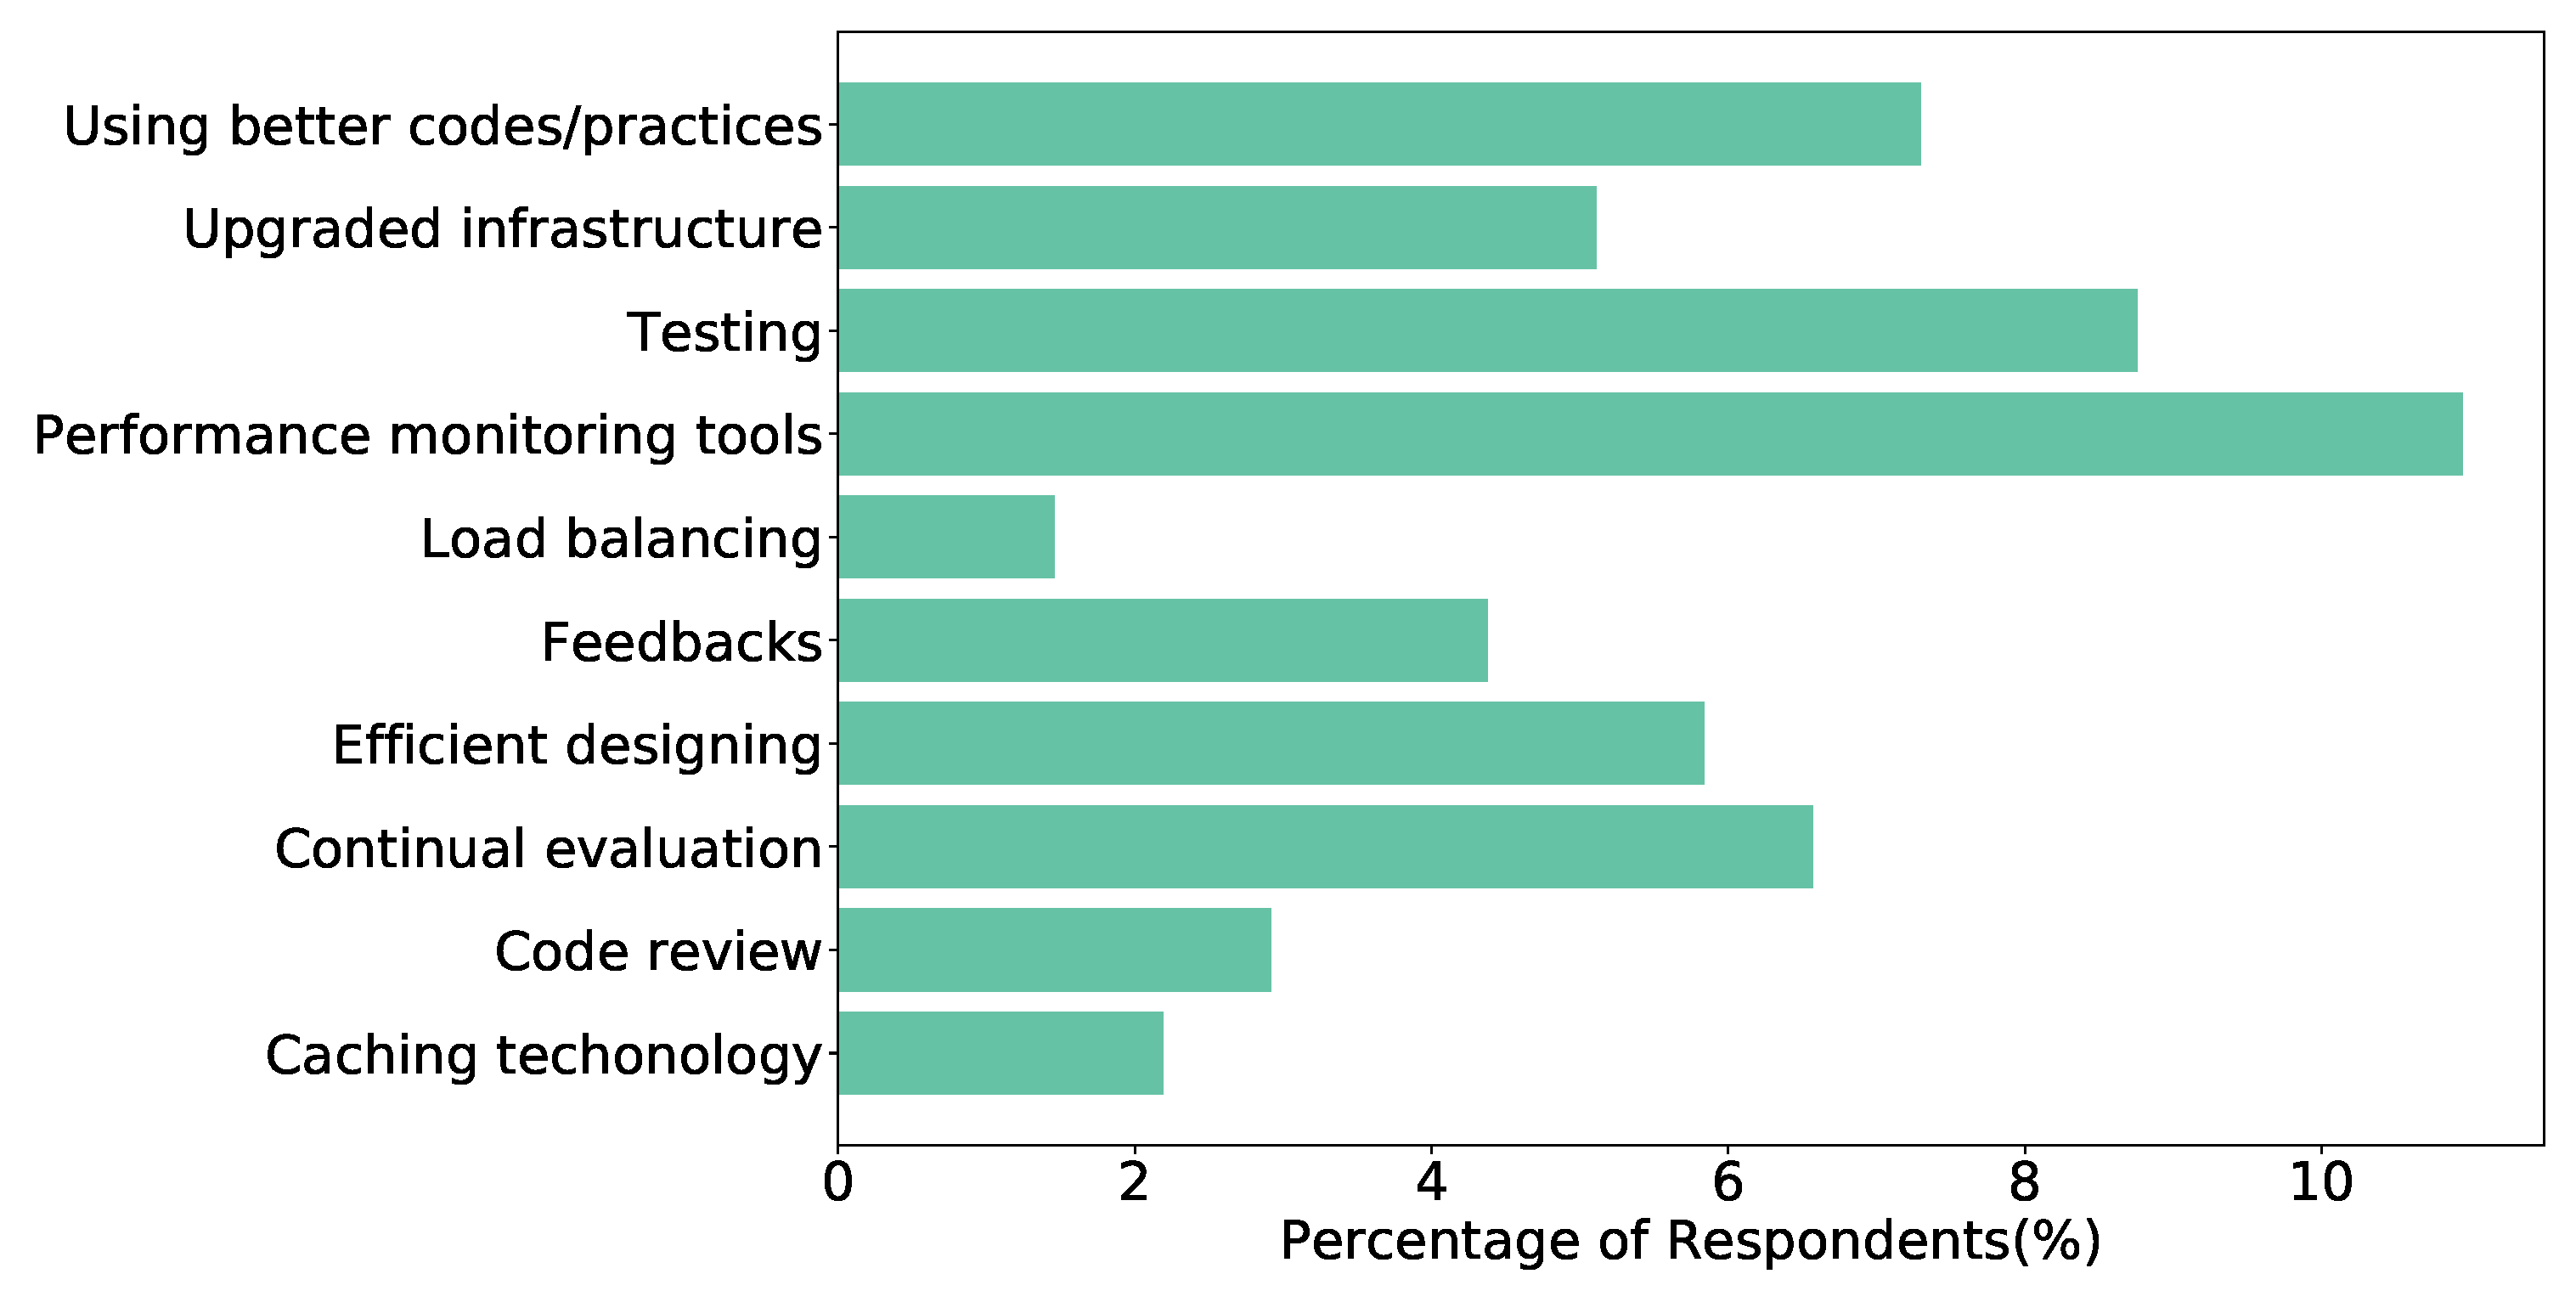
\includegraphics[scale=0.28]{Figures/Performance.eps} 
% \caption{Measures to ensure performance of products}
% \label{fig:Measures to ensure performance}
% \end{figure}
% \hfill\\

Software performance indicates how efficient the software is in terms of resources and time. Use of framework/tools/platform to ensure software performance is a dominant practice in the Bangladesh SE industry. The other type of practices is peer-review, software design, and software testing. Respondents in our survey reported multiple measures under these categories. The measures in \emph{framework/tools/platform} category are,
\begin{enumerate}[label=(\alph*)]

    \item \textbf{Load Balancing}: Load balancing can improve the system performance by ensuring an equal load to all servers. 27.1\% of respondents think of using load balancing as a measure to maintain performance.
    \surveyquote{Optimizing number of HTTP requests, Asynchronous programming, Caching, CDN, Load Balancing, nginx, varnish, compression of data, Continuous monitoring, Load testing, stress testing}{42}
    
    
    \item \textbf{Performance Monitoring Tools}: There are various performance monitoring automated tools from which we can measure the overall and component-wise performance. 10.95\% of respondents use these tools to measure performance. Respondents use several performance metrics such as error/crash rate, response time, uptime, etc.
    \surveyquote{take help of different performance monitoring tools and dashboard, analyzed data , measure time and memory efficiency of process}{35}
    
    \item \textbf{Upgraded Infrastructure}: 5.11\% of respondents use upgraded infrastructure to ensure performance. This infrastructure includes cloud hosting, a high-end server, and new technologies.
    \surveyquote{Amazon Hosting and Quality Software}{85}
    
    \item \textbf{Caching Technology}: Caching mechanism improves performance by reducing response time. 2.92\% of respondents rely on caching to maintain software performance.
    \surveyquote{... Good Caching}{29}

\end{enumerate}


13.14\% of respondents ensure software performance  at design phase. Measures of this category are,

\begin{enumerate}[label=(\alph*)]

    \item \textbf{Using better codes/practices}: Industry-standard best practices can improve system performance. 7.3\%respondents ensure performance by implementing best practices. The best practices include compression technology, enforcing design patterns, and refactoring.
    \surveyquote{Implementation time carefulness and maintaining a well developed coding standard}{40}
    
    \item \textbf{Efficient designing}: Software performance is dependent on the architecture of the system. 5.84\% of respondents emphasize design to ensure performance.
    \surveyquote{By careful designing}{24}

\end{enumerate}

 8.76\% of respondents of our survey rely on the software testing strategy to ensure performance. Performance is ensured by various rigorous testing phase. The phase includes load testing, stress testing, integration testing.
 \surveyquote{By rigorous testing and checking performance testing}{17}
 
 Reviewing peer and user, tester feedback can be a good strategy to ensure performance. 7.3\% of our respondents use measures from this category to ensure performance. Measures under this category are,
 
 \begin{enumerate}[label=(\alph*)]
 
     \item \textbf{User Feedback}: It is a great source of performance measure. Taking time to time feedback from the clients helps a company realize how their products are performing. Many (4.38\%) respondents have highly recommended it.
    \surveyquote{Continuous feedback from clients and QA team}{65}
    
    \item \textbf{Code Review}: About 2.92\% of people have said that a proper and attentive code review can reduce the codes' faults and, therefore, enhance the performance of a software.
    \surveyquote{The code quality is assessed by the different team members during code review, followed by designing new ways to solve issues in the product that are time-intensive.}{15}
 
 \end{enumerate}



\paragraph{Scalability}
% \label{Scalability}
% \begin{figure}[htbp]
% 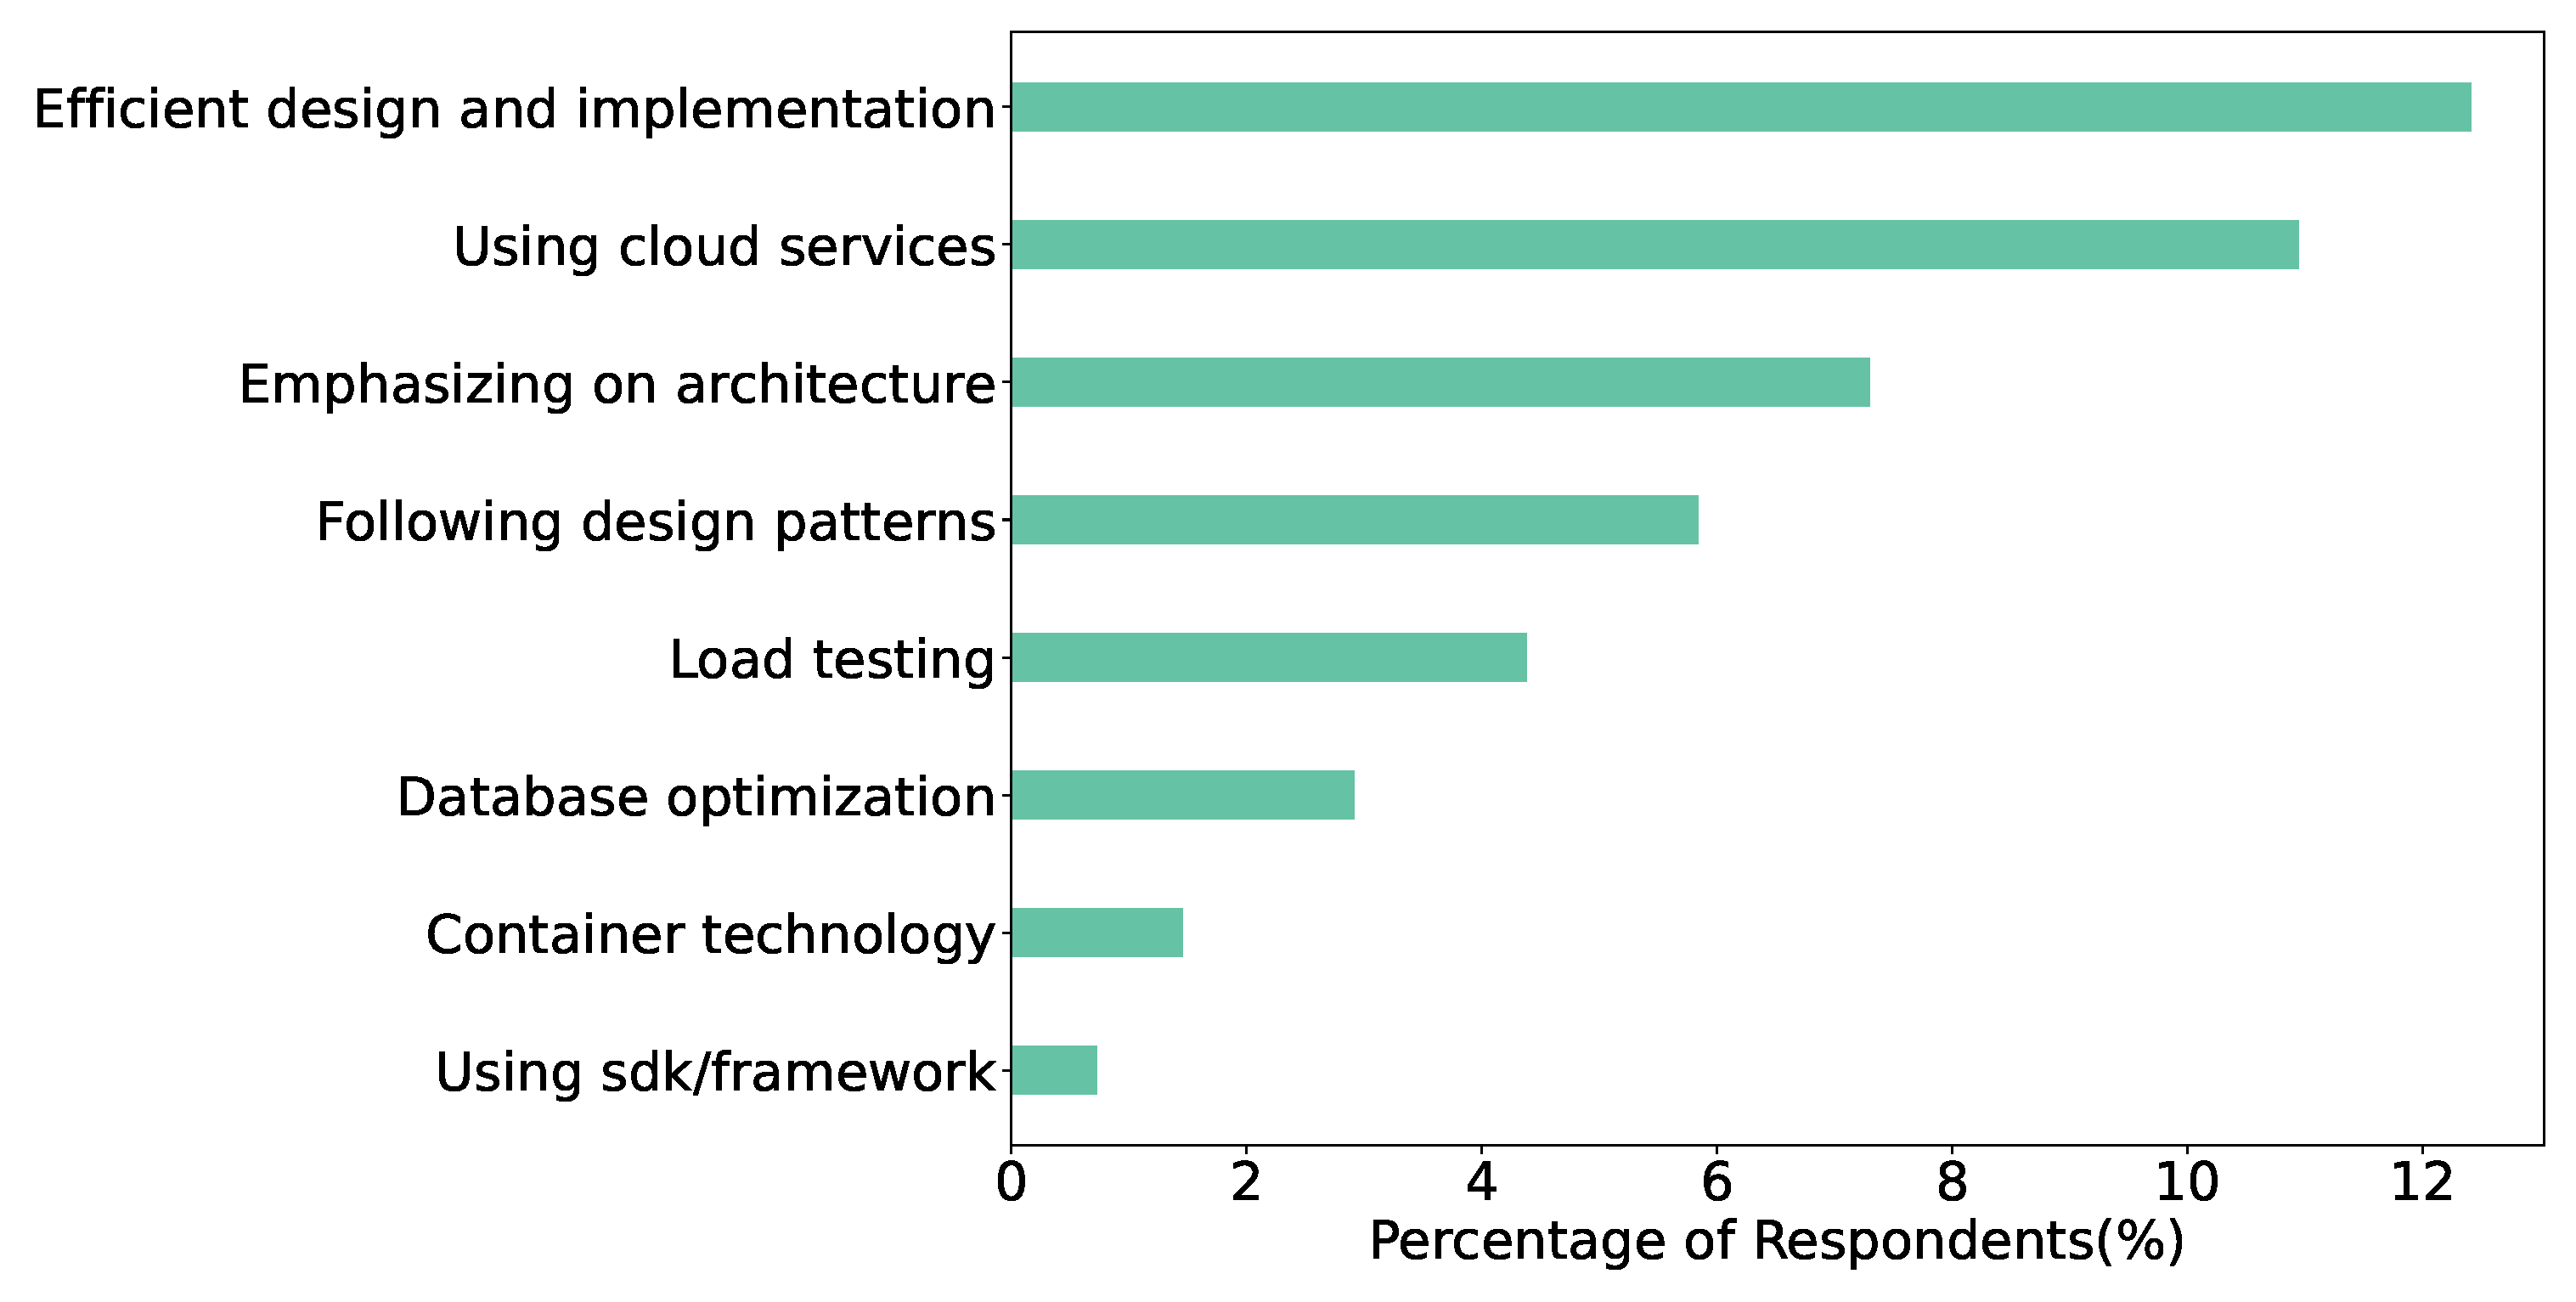
\includegraphics[scale=0.28]{Figures/Scalability.eps} 
% \caption{Measures to ensure scalability of products}
% \label{fig:Measures to ensure scalability}
% \end{figure}
% \hfill\\

 Software scalability defines the ability to scale up a solution. Issues with little importance can impede scaling up. Thus proper measures should be taken from the design stage to ensure the scalability of the system. Scalability ensured by efficient software design is the most practices strategy in the Bangladesh SE industry. 25.55\% reported using at least one of the measures in this category. The measures are,
% Recent days the cloud services offer tools to accomodate custom reactive scaling strategies. Thus, it has become easier to ensure scalability using cloud services \cite{Falatah2014}. Our results  also follows the world trend, usage of cloud services has placed 2\textsuperscript{nd} in terms popularity of scalability measures in SE industry of Bangladesh.
 \begin{enumerate}[label=(\alph*)]
 
     \item \textbf{Efficient Design and Implementation}: 12.41\% of respondents emphasize on the design and implementation of a scalable architecture. 
    \surveyquote{During implementation we always keep in mind about the scaling factor}{40}
    
     \item \textbf{Emphasizing on architecture}: 7.3\% of respondents emphasized on architecture. It is mostly micro-service architecture which they use to ensure scalability.
    \surveyquote{We follow the micro-service architecture. In a nutshell, we scale up the module vertically which is necessary. We use docker along with Jenkins for automatic deployments and scaling.}{10}

    
    \item \textbf{Following Design Patterns}: Some design patterns inherently help in the time of scaling. 5.84\% of respondents think that following these design patterns will be of great use for software scalability.
    \surveyquote{Following certain design patterns}{8}
 
 \end{enumerate}
 
 13.14\% of respondents of our survey use framework or some kind of tool to ensure scalability. The measures in this category are,
\begin{enumerate}[label=(\alph*)]

    \item \textbf{Using Cloud Services}: 10.95\% user depends on cloud services like AWS and Azure for the scalability of the system. Modern features like elastic load balancing and auto-scaling make it easy to ensure scalability.
    \surveyquote{Using AWS Elastic Load Balancer}{28}
    
    \item \textbf{Container Technology}: Container technologies include Docker, Kubernetes, which ensure OS-level virtualization. By standardizing the system, container technologies ease the scaling of an infrastructure.1.46\% of respondents use these measures to ensure product scalability. Containers enable users to scale their system without any worries about the underlying OS.
    \surveyquote{We used Docker technology}{85}
    
    \item \textbf{Using SDK/framework}: Modern frameworks ensure scalability by default. 0.73\% of respondents solely depend on the framework for scalability.
    \surveyquote{following flexible framework which allows better scalability}{14}
  
\end{enumerate}
 
 
There is one measure under the software testing category, which is load testing. Load testing can be used to check the scalability of a system. 4.38\% of respondents use load tests to check whether their system is scalable or not.
\surveyquote{through load testing and load simulation.}{35}

There is also one measure under the Database Design category, which is database optimization. Database optimization includes sharding, clustering, indexing, and scaling. 10.3\% of respondents optimize database to scale their system.
\surveyquote{Besides scaling horizontally, database scaling is performed by partitioning tables, along with multi-threaded implementations}{85}


% \subsection{Comparison among countries (RQ2)}
\label{RQ2}

In this section, we present a comparative discussion on different dimensions of software development practices and processes among different regions of the world along with Bangladesh. We do the comparison along the following dimensions:

\begin{itemize}
    \item Development methods and practices
    \item Implementation technologies
    \item Quality assurance
    \item Release and iterations
\end{itemize}

The following subsections describe these dimensions.

\subsubsection{Development methods and practices}
\label{dev_methods}

To find out the overall comparison of this section, we report the following sub-sections:

\begin{itemize}
\item Software development methodologies (Q 6).
\item Requirements gathering (Q 7).
\item Most time consuming software development activities (Q 8).
\end{itemize}

\paragraph{Software development methodologies}
From the study we see that the most acceptable model that was regularly and always used is the agile model (64\%) in Bangladesh but the usage of the scrum (44\%) in New Zealand has greater usage followed by agile (30\%) \cite{Wang2018} and in Turkey, waterfall is mostly used based on the earlier 2015 survey \cite{Garousi2015}. Again, in both Bangladesh and New Zealand, extreme programming (XP) has a lower percentage of usage.

\paragraph{Requirements Gathering}
According to \ref{fig:requirements}, using plain text (44\%) and story board (41\%) are the most widely used requirements gathering. This result is similar with the survey of Vonken et al. \cite{Vonken2012}. From their study we can find that the textual description of specifying requirements is a firm favourite in Netherlands.

\paragraph{Development activities timeline}
According to study \cite{Wang2018}, most time was spent on implementation and coding and also relatively less time was spent on maintenance in both Bangladesh and New Zealand. But requirement analysis, the activity, requires the second most time to spend in Bangladesh according to 45\% respondents where in New Zealand, it is testing (36\%) practices.

\subsubsection{Implementation technologies and tools}
\label{implementaion_techonologies}

To find out the overall comparison of this section, we report the following sub-sections:
\begin{itemize}
\item Technology Platform (Q 9).
\item Operating System (Q 10).
\item Programming Language (Q 11).
\end{itemize}


\paragraph{Technology Platforms}
As shown in \ref{fig:platforms}, most of the respondents (80\%) worked in web platform. Most respondents develop products and services for web platforms in both Bangladesh and New Zealand based on \cite{Wang2018}.

\paragraph{Operating Systems}
Windows is mostly used among developers of New Zealand based on the survey \cite{Wang2018}, but Linux is mostly used in the case for Bangladeshi developers.

\paragraph{Programming Languages}
Based on \cite{Wang2018}, Java ranks quite low in New Zealand where it is the second most used in Bangladesh and the mostly used language in Turkey \cite{Garousi2015}. Again, python did not get a respective place in the rank of used languages in New Zealand but it is used significantly in Bangladesh.

\subsubsection{What type of testing and deployment practices are used?}

To get the picture of quality assurance (QA) in countries such as Malaysia, Turkey, France, etc., different studies have been carried out. In Table \ref{table:testing_comparison}, we compare the major outcomes of testing and deployment related responses from our study with the similar results of the previous studies. The comparative picture is discussed below.

\begin{itemize}
    % \item Requirements Clarity
    \item Software Testing Practices (Q14)
    \item Level of Automated Testing (Q15)
\end{itemize}

\input{Tables/testing_comparison}


\paragraph{Software Testing Practices}
From our study, as per \ref{fig:testing}, we see an interesting point that unit testing (53\%) and functional testing (49\%) are moderately used in Bangladesh, whereas from \citep{Garousi2013} and \citep{Wang2018} we can see that relatively a high percentage of their survey respondents in both Canada New Zealand rely on unit testing with 79.27\% and 73\% respectively. On the other hand, the adoption of acceptance testing and UI testing is quite similar to these countries. In Malaysia, based on \citep{Baharom2006}, Baharom et al. reported that, according to their survey, unit testing (68.29\%), integration testing (78.05\%), system testing (85.37\%), and acceptance testing (78.05\%) are used by most organizations in a high percentage, and about half of the organizations are carrying out alpha and beta testing.

\boxtext{Software developers around the world usually give unit testing the top priority, but the developers in Bangladesh have comparatively less participation.}
\rifat{Is the above observation correct? 53\% usage of unit testing reported.}\khalid{added percentages. The response rate of unit testing in our survey lags compares to others. Is it okay now?}

\paragraph{Level of Automated Testing}
We have found that as per \ref{fig:autoTest}, around 25\% of our respondents are highly concerned that they have to use automated testing for their projects, while around 35\% of our respondents have expressed medium level concern and the remaining are hardly concerned about using automated testing. From the study of Dutta et al. \citep{dutta1999}, we have found that in automated testing practices, Bangladesh is quite similar to all of Europe but lags behind France. According to their study, the usage rate of automation testing tools in overall Europe is 26\%, where in France, it is as high as 61\%. But in Israel, this rate is the only 9\%.

\begin{tcolorbox}[flushleft upper,boxrule=1pt,arc=0pt,left=0pt,right=0pt,top=0pt,bottom=0pt,colback=white,after=\ignorespacesafterend\par\noindent]
\nd\it{\bf{RQ2-D3. Software testing and devops practices used.}} 
\gias{summarize}
\end{tcolorbox}

\subsubsection{Release and Iterations}
\label{vcs_comparison}

\subsubsection{Security measures}
\label{security_comparison}

3.64\% of our survey respondents reported not to use any security measures in their product. This practice is also prevalent in the Indian and Malaysian software industries. Bahl et al.\cite{Bahl2011} reported that due to misalignment with organization design, goal, and strategy in some Indian software firms, security measures are not practiced. In a study on  Malaysian developers, Farvin et al.\cite{Farvin2016} found that 31\% of respondents think it is not required to add security in requirement analysis of a product. Basharat et al.\cite{Basharat2013} reported a sense of false security in the small software industry, and standard security practices are hardly followed. This can be one reason why some Bangladesh software industry respondents do not use any security measures.  From the response of a survey on the Turkey software industry, Garousi et al.\cite{Garousi2015} ranked types of design activities in terms of frequency. In that rank, security architecture was ranked second out of five. The ranking represents that security architecture is not a frequent activity in the Turkish software industry. However, in our survey, a very few (2.19\%) respondents reported practicing security architecture.  Bangladesh, the Turkish, and the New Zealand software industry have a resemblance in the practice of security testing. Garousi et al.\cite{Garousi2015} reported that security testing is least widely used among all kinds of testing ( e.g., unit testing, integration testing). Sung et al.\cite{Sung2006} found that in the New Zealand software industry, security testing and recovery testing practices are negligible compared to functional testing. The scenario is the same for Bangladesh; we found that 6.57\% of respondents reported security testing to ensure security.


\subsubsection{Performance measures}
\label{performance_comparison}
8.76\% of respondents of our survey use performance testing to ensure the performance of their product. However, it is the second least practiced measure among all the measures. Garousi et al.\cite{Garousi2015} found that in the Turkish software industry, developers mark the lack of performance testing as the main challenge in software maintenance. However, the scenario is different for the Canadian software industry. Participants of the survey of Garousi et al.\cite{Garousi2013} reported that 40\% of them conduct performance testing, and 30\% of their total testing effort is spent on performance testing. The New Zealand software industry follows the Canadian practice. Phillips et al.\cite{Phillips2003} reported that performance testing is a common testing practice in New Zealand. However, the practice of the Bangladeshi software industry matches the practices of the Pakistan software industry. In Pakistan software industry, performance testing is hardly practiced. In the survey of Shah Jahan et al.\cite{Jahan2019}, only 5\% of participants reported conducting performance testing. It seems that performance testing is less popular in growing software industries such as Bangladesh and Pakistan.

Peer review is the least practiced measure in the Bangladesh SE industry. However, in the Turkish SE industry, peer review is ranked as the most frequent activity\cite{Garousi2015} (ranked five on a five-point Likert scale). Though the practice is only limited to code review. In architecture/design review is  hardly practiced in turkey (ranked one in a five-point Likert scale)

\subsubsection{Scalability measures}
\label{scalability_comparison}
There is no study focusing on scalability practices in specific software industries, so it is difficult to compare scalability practices. However, in a study on Finnish DevOps, Laihonen\cite{Laihonen2018} found that the Finnish software industry prefers cloud services as it helps them automate quality insurance. He also reported that DevOps are inclined towards micro-service architecture when selecting a product rather than monolith architecture. Hussain et al.\cite{Hussain2017} conducted a study to identify trends in the DevOps practices in New Zealand. For this study, besides interviewing the DevOps', they examined the job advertisements for a DevOps role. They found that containerization technologies (e,g.; Docker, Kubernetes) have a high demand in the New Zealand software industry. 94\% of job advertisement requires expertise in one or multiple containerization technologies. This indicates the popularity of docker technology in the New Zealand software industry. However, in the Bangladesh SE industry, the scenario is different. Cloud services are the second most popular (10.95\%)  measure to ensure scalability where the use of containerization technologies are not that much popular (1.46\%)


\section{Discussions}
\label{discussions}


\subsection{Challenges and Opportunities}
\label{dicussion challanges}
% open ended question - scalability, security and performance
% now summarize the key finding - see Section 7.1 of \url{https://ieeexplore.ieee.org/abstract/document/8658125}


3.64\% of our respondents responded that they do not take any measures to mitigate the security risk. The common reason for not taking any measures is (1) the product is an early stage (2) the respondents' role does not require any measures regarding product security. The reason for not taking any security measures is different from North America\cite{Assal2019}; there, the first reason is that there are no formal test plans. The second one is the lack of knowledge regarding testing tools. Though respondents do not think about product security initially, it is recommended\cite{Chandra2009,Azham2011} to plan security tests and product security from the design phase.

Modern frameworks provide the basic security of the solution. Moreover, some framework provides enhanced, focused, customized security through a plug-in or add-on, e.g., spring-security, spring-cloud security. Framework-based security is a growing practice in the software industry\cite{Alssir2012}.  The practice in the Bangladesh SE industry matches the global practice. According to our survey, it is the second most popular measure to mitigate security risk. Survey respondents have reported using OWASP, HDIV, and spring security. Srinivasan et al.\cite{Srinivasan2017} has conducted a comparison among the popular web frameworks based on security. Based on five criteria, they ranked the frameworks, and all of the mentioned frameworks of our respondents are in the top 10 list. It seems that secure software engineering practice is prevalent in the Bangladesh SE industry.


On a survey of 237 software professionals, Elahi et al.\cite{Elahi2011} found that 51\% of respondents maintain at least one security standard, and 19\% of respondents maintain ISO 17799 security standard. On the contrary, about 10.22\% of respondents of the Bangladesh software industry maintain any security standard. It is clear that security standards are not that much popular in this SE industry.

According to Smith et al.\cite{Smith2003}, efficient architecture and continuous monitoring tools are two of the twenty-four best practices to ensure software performance.  The respondents report both practices. However, Smith et al. presented twenty-one other best practices, and we have not found other practices in our survey. It is clear the SE industry of Bangladesh only practices a few best measures for ensuring software performance.

27.1\% of respondents in our survey reported that they use the load balancer to ensure software performance. A load balancer is mostly used to reduce queue time/ response time in web base application\cite{Mesbahi2016}. Thus we can infer that most of our survey respondents mainly engaged in developing the web-based application.


Bondi et al.\cite{Bondi2000} has listed four scalability types to ensure software capability to scale; however, we observe only one type of scalability (load scalability) in our responses. To obtain software scalability use of cloud services is one of the most popular strategies\cite{Gao2011}. Another popular strategy is the use of microservice. Microservice and cloud services together allow the user to scale up and down any system dynamically. Cáceres et al.\cite{Cceres2010} reported that cloud services and microservice-based architecture are generally used together to ensure scalability. In the Bangladesh SE industry, this practice may be prevalent. The use of cloud service and efficient use of architecture are the second and third most popular topic among our respondents.

\subsection{Analysis by Professions}
\label{analyze_by_professions}
% summarize key findings by professions. see Section 7.2 of \url{https://ieeexplore.ieee.org/abstract/document/8658125}
In Tables \ref{table:analysis by profession part1}, \ref{table:analysis by profession part2}, and \ref{table:analysis by profession part3}, we summarize the interesting results of our survey's closed questions by survey participants' reported roles. We report each question as follows:

\begin{enumerate}[label=\arabic*)]
    \item Multiple Choice Questions. If the question has two options (Male, Female), we only show the result of the option(s) with the majority agreement.
    \item For all other questions, we reported the top two values for each role. For example, for the question ‘Which of the following do you use for requirements gathering?’ in Table \ref{table:analysis by profession part1}, we reported PT (Plain Text) and SB (Story Board) for the software engineer's role. 26.2\% of software engineers use PT, and 22.99\% use SB. These two requirements gathering process are the top two among all the other process used by software engineers.
\end{enumerate}

\newcolumntype{b}{X}
\newcolumntype{v}{>{\hsize=.03\hsize}X}
\newcolumntype{m}{>{\hsize=.2\hsize}X}
\newcolumntype{y}{>{\hsize=.33\hsize}X}
\begin{table}[htbp]
    \centering
    \caption{Highlights of Findings from Survey Closed Questions by Profession}
    \begin{tabularx}{\textwidth}{v|b}
        \hline
        \textbf{No}     & \textbf{Question}  \\ \hline
        4         & For how many years have you coded professionally?\newline 1) Architect: \textbf{\textit{more than 10, 100.0\% } } 2) Business analyst: \textbf{\textit{more than 10, 100.0\% } } 3) Data Engineer: \textbf{\textit{more than 10, 100.0\% } } 4) Developer: \textbf{\textit{less than 2, 41.41\% } } 5) Manager: \textbf{\textit{more than 10, 58.33\% } } 6) R\&D: \textbf{\textit{less than 2, 100.0\% } } 7) SQA: \textbf{\textit{2 to 5, 50.0\% } } 8) Team Lead: \textbf{\textit{5 to 10, 100.0\% } } 9) Trainer: \textbf{\textit{2 to 5, 100.0\% } } 10) UXD: \textbf{\textit{5 to 10, 100.0\% } }    \\ \hline
        
        
        6         & Which of the following software development methodologies do you follow?\newline 
        {
        \begin{tabularx}{0.92\textwidth}{yyy}
         & top1 (\%) & top2 (\%) \\
        Architect & Agile (100.0)  &  \\
        Business analyst & Agile (33.33)  & Scrum (33.33)  \\
        Data Engineer & Scrum (100.0)  &  \\
        Developer & Agile (42.0)  & Scrum (32.67)  \\
        Manager & Agile (37.29)  & Scrum (28.81)  \\
        R\&D & Scrum (66.67)  & Agile (33.33)  \\
        SQA & Agile (53.33)  & Scrum (20.0)  \\
        Team Lead & Agile (100.0)  &  \\
        Trainer & Agile (25.0)  & Pair Programming (25.0)  \\
        UXD & Agile (50.0)  & Scrum (50.0)  \\
        \end{tabularx}
        }
        \\ \hline
        7 & Which of the followings do you use for requirements gathering?\newline
        GUI prototype = GP, Grooming seasons = GS, Plain Text = PT, Story board = SB, Use Case = UC
        {
        \begin{tabularx}{0.92\textwidth}{yyy}
         \\
         & top1 (\%) & top2 (\%) \\
        Business analyst & GP (22.22)  & GS (22.22)  \\
        Data Engineer & PT (33.33)  & SB (33.33)  \\
        Developer & PT (26.2)  & SB (22.99)  \\
        Manager & GS (20.48)  & SB (20.48)  \\
        R\&D & GS (33.33)  & SB (33.33)  \\
        SQA & UC (27.78)  & GS (22.22)  \\
        Team Lead & GP (33.33)  & SB (33.33)  \\
        Trainer & GP (25.0)  & PT (25.0)  \\
        UXD & GP (50.0)  & UC (50.0)  \\
        \end{tabularx}
        }
        \\ \hline
        8 & On which software development activities, do you spend most of the time?\newline Program Design = PD, Requirement Analysis = RA
        {
        \begin{tabularx}{0.92\textwidth}{yyy}
        \\
         & top1 (\%) & top2 (\%) \\
        Architect & Implementation (25.0)  & PD (25.0)  \\
        Business analyst & Implementation (33.33)  & RA (33.33)  \\
        Data Engineer & Implementation (33.33)  & Maintenance (33.33)  \\
        Developer & Implementation (30.33)  & RA (18.85)  \\
        Manager & RA (22.37)  & Implementation (21.05)  \\
        R\&D & Implementation (50.0)  & PD (50.0)  \\
        SQA & Testing (25.0)  & RA (17.86)  \\
        Team Lead & Documentation (25.0)  & Implementation (25.0)  \\
        Trainer & Implementation (25.0)  & PD (25.0)  \\
        UXD & Implementation (33.33)  & Maintenance (33.33)  \\
        \end{tabularx}
        }\\ \hline
    \end{tabularx}
    \label{table:analysis by profession part1}
\end{table}
% \newcolumntype{b}{X}
\newcolumntype{v}{>{\hsize=.03\hsize}X}
\newcolumntype{k}{>{\hsize=.97\hsize}X}
\begin{table}[!ht]
    \centering
    \caption{Highlights of Findings from Survey Closed Questions by Profession}
    \begin{tabularx}{\textwidth}{v|k}
        \hline
        \textbf{No}     & \textbf{Question}  \\ \hline
        9 & Which of the following technologies do you have experience working in?\newline
        1) Architect: Mobile (50\%) 2) Business analyst: Desktop (33.33\%) 3) Data Engineer: Others (100\%) 4) Developer: Web (49.39\%) 5) Manager: Web (36.92\%) 6) R\&D: Web (66.67\%) 7) SQA: Web (40.91\%) 8) Team Lead: Desktop (50\%) 9) Trainer: Desktop (33.33\%) 10) UXD: Web (100\%)\\ \hline
        10 & What is the primary operating system you are developing on?\newline
        1) Architect: Linux (66.67\%) 2) Business analyst: Windows (66.67\%) 3) Data Engineer: MacOS (100\%) 4) Developer: Linux (42.86\%) 5) Manager: Linux (53.49\%) 6) R\&D: Linux (50\%) 7) SQA: Windows (56.25\%) 8) Team Lead: Windows (100\%) 9) Trainer: Others (100\%) 10) UXD: Linux (50\%) \\ \hline
        
        11 & Which programming languages are you using?\newline
        1) Architect: Java (100\%) 2) Business analyst: JavaScript (40\%) 3) Data Engineer: Go (25\%) 4) Developer: JavaScript (31.75\%) 5) Manager: JavaScript (27.06\%) 6) R\&D: Java (66.67\%) 7) SQA: Java (24\%) 8) Team Lead: C\# (25\%) 9) Trainer: C/C++ (25\%) 10) UXD: JavaScript (100\%) \\ \hline
        12 & Which frameworks are you using? \newline
        1) Architect: Spring (100\%) 2) Business analyst: ASP. NET (16.67\%) 3) Developer: Spring (26.61\%) 4) Manager: Spring (23.73\%) 5) R\&D: Spring (66.67\%) 6) SQA: ASP. NET (25\%) 7) Team Lead: ASP. NET (50\%) 8) Trainer: Django (100\%) \\ \hline
    \end{tabularx} 
    \label{table:analysis by profession part2}
\end{table}
\newcolumntype{b}{X}
\newcolumntype{v}{>{\hsize=.03\hsize}X}
\newcolumntype{m}{>{\hsize=.2\hsize}X}
\newcolumntype{y}{>{\hsize=.33\hsize}X}
\begin{table}[!ht]
    \centering
    \caption{Highlights of Findings from Survey Closed Questions by Profession}
    \begin{tabularx}{\textwidth}{v|b}
        \hline
           13 & What types of software testing practices do you use? \newline
           1) Architect: Functional testing (25\%) 2) Business analyst: Unit testing (40\%) 3) Data Engineer: Performance testing (50\%) 4) Developer: Unit testing (27.81\%) 5) Manager: Unit testing (23.33\%) 6) R\&D: Performance testing (50\%) 7) SQA: Functional testing (20.93\%) 8) Team Lead: Functional testing (33.33\%) 9) Trainer: Functional testing (25\%) \\ \hline
           
           15 & What is the level of automated testing in your projects?\newline
           1) Architect: 3 (100\%) 2) Business analyst: 1 (50\%) 3) Data Engineer: 2 (100\%) 4) Developer: 5 (40.66\%) 5) Manager: 2 (36.36\%) 6) R\&D: 3 (50\%) 7) SQA: 3 (44.44\%) 8) Team Lead: 4 (100\%) 9) Trainer: 4 (100\%) 10) UXD: 4 (100\%) \\ \hline
           16 & Which tools do you use for testing and quality assurance?\newline
           1) Architect: Selenium (50\%) 2) Business analyst: JenKins (33.33\%) 3) Data Engineer: XUnit (100\%) 4) Developer: XUnit (35.14\%) 5) Manager: XUnit (34.88\%) 6) R\&D: Selenium (50\%) 7) SQA: Selenium (43.75\%) 8) Team Lead: Selenium (50\%) 9) Trainer: JenKins (100\%)\\ \hline
           17 & Which tools do you use for continous deployment? \newline
           1) Business analyst: Jenkins (100\%) 2) Developer: AWS codeDeploy (25.45\%) 3) Manager: Jenkins (31.03\%) 4) R\&D: Open Source server (100\%) 5) SQA: Bamboo (60\%) 6) UXD: AWS codeDeploy (100\%) \\ \hline
           
        
    \end{tabularx} 
    \label{table:analysis by profession part3}
\end{table}

The agile method is the most practiced software requirement method in Bangladesh. It is popular among respondents of almost all positions. The second popular method is Scrum.
\boxtext{Agile is the most practiced requirement gathering method. The popularity of Agile method is consistent across the different reported roles in our surveys.}

In Q8, participants were asked to identify the SDLC activity, where most of the time is spent. Generally, it is expected that participants in the senior role (e.g., manager, team lead) will spend time in requirement analysis, documentation where participants in the junior role (e.g., developers, r\&d engineer) will spend time in implementation and testing. From  Q8 in Table \ref{table:analysis by profession part2}, we observe that senior roles participants mostly spend time in requirement analysis and documentation. However, testing is not in the top two most times spent activity. For participants in the junior role, the second-most time-consuming activity includes several other SDLC steps (e.g., maintenance, requirement analysis, etc.). This may indicate that in Bangladesh, SE industry testing is considered comparatively less important.
\boxtext{Across all roles, implementation is the most time spent activity in SDLC. However, testing is not considered one of the most time-consuming activities. Rigorous testing practices may not be prevalent in the Bangladesh SE industry.}

Across all the roles Java and JavaScript are the top two most used languages (java is the second most used language in cases where javascript is the most used language). Even in the data engineer role, Java is the most used language, though python is mostly used in the data processing. Like Java, Spring (one framework of Java) is the widely used framework regardless of role.
\boxtext{Java and JavaScript are the most used languages regardless of role}

From Q14 of Table \ref{table:analysis by profession part3}, we observe that developers mostly practice the highest automated testing level. In Q13 of Table \ref{table:analysis by profession part3}, we observe that developers mostly practice unit testing. It is comparatively easier to achieve automated testing in unit testing because of several testing frameworks. This may be one of the reasons behind the high level of automated testing among developers. Automated tests offering libraries/frameworks for other types of testing can encourage higher automated testing levels in other roles.
\boxtext{Developers mostly practice the highest level of automated testing. Automated testing framework for other types of testings may increase the practice of automated testing.}


\subsection{Analysis by Experience}
% see Section 7.3 of \url{https://ieeexplore.ieee.org/abstract/document/8658125}

We highlight the results of our survey's closed questions by the reported professional experiences of the survey respondents in Table \ref{table:analysis_by_experience_part1} and \ref{table:analysis_by_experience_part2}. The similar principles discussed in Section \ref{analyze_by_professions} are applied for this report.

% \newcolumntype{b}{X}
\newcolumntype{v}{>{\hsize=.04\hsize}X}
\newcolumntype{k}{>{\hsize=.96\hsize}X}
\newcolumntype{m}{>{\hsize=.2\hsize}X}
\newcolumntype{y}{>{\hsize=.33\hsize}X}
\begin{table}[!ht]
    \centering
    \caption{Highlights of Findings from Survey Closed Questions by Experience}
    \begin{tabularx}{\textwidth}{v|k}
        \hline
        \textbf{No}     & \textbf{Question}  \\ \hline
        5 & What is your current role?\newline 1) less than 2: Developer (91.11\%) 2) 2 to 5: Developer (75.0\%) 3) 5 to 10: Developer (60.71\%) 4) more than 10: Manager (42.42\%) \& Developer (42.42\%) \\ \hline
        
        6 & Which of the following software development methodologies do you follow?\newline 
        1) less than 2: Agile (55.74\%) 2) 2 to 5: Scrum (34.78\%) 3) 5 to 10: Agile (50.0\%) 4) more than 10: Agile (33.33\%) \\
        % {
        % \begin{tabularx}{0.92\textwidth}{yyy}
        %     & top1 (\%) & top2 (\%) \\
        % less than 2 & Agile (55.74)  & Scrum (27.87)  \\
        % 2 to 5 & Scrum (34.78)  & Agile (30.43)  \\
        % 5 to 10 & Agile (50.0)  & Scrum (30.0)  \\
        % more than 10 & Agile (33.33)  & Scrum (31.67)  \\
        % \end{tabularx}
        % } \\
        \hline
        
        7 & Which of the followings do you use for requirements gathering?\newline
        1) less than 2: Plain Text (30.88\%) 2) 2 to 5: Plain Text (29.03\%) 3) 5 to 10: Story board (23.73\%) 4) more than 10: Story board (27.63\%) \\
        % GUI prototype = GP, Grooming seasons = GS, Plain Text = PT, Story board = SB, Use Case = UC
        % {
        % \begin{tabularx}{0.92\textwidth}{yyy}
        %     & top1 (\%) & top2 (\%) \\
        % less than 2 & PT (30.88)  & UC (20.59)  \\
        % 2 to 5 & PT (29.03)  & GP (20.97)  \\
        % 5 to 10 & SB (23.73)  & GS (20.34)  \\
        % more than 10 & SB (27.63)  & UC (19.74)  \\
        % \end{tabularx}
        % }   \\ 
        \hline
        
        8 & On which software development activities, do you spend most of the time?\newline Implementation = Imp, Requirement Analysis = RA
        {
        \begin{tabularx}{0.92\textwidth}{yyyy}
            & top1 (\%) & top2 (\%) & top1 / top2 \\
        less than 2 & Imp (29.9)  & RA (19.59) & 1.53 \\
        2 to 5 & Imp (32.88)  & RA (15.07) & 2.18  \\
        5 to 10 & Imp (21.69)  & RA (19.28) & 1.125 \\
        more than 10 & Imp (23.68)  & RA (23.68) & 1 \\
        \end{tabularx}
        }\\ \hline
        
        9 & Which of the following technologies do you have experience working in?\newline
        1) less than 2: Web (51.43\%) 2) 2 to 5: Web (56.0\%) 3) 5 to 10: Web (46.0\%) 4) more than 10: Web (35.38\%)
        % {
        % \begin{tabularx}{0.92\textwidth}{yyy}
        %     & top1 (\%) & top2 (\%) \\
        % less than 2 & Web (51.43)  & Mobile (24.29)  \\
        % 2 to 5 & Web (56.0)  & Mobile (26.0)  \\
        % 5 to 10 & Web (46.0)  & Mobile (30.0)  \\
        % more than 10 & Web (35.38)  & Mobile (29.23)  \\
        % \end{tabularx}
        % }\\ 
        \\ \hline
        
        10 & What is the primary operating system you are developing on?\newline
        1) less than 2: Windows (46.15\%) \& Linux (30.77\%), 2) 2 to 5: Linux (47.73\%) \& Windows (38.64\%), 3) 5 to 10: Linux (41.46\%) \& Windows (26.83\%), 4) more than 10: Linux (52.27\%) \& MacOS (25.0\%)
        % {
        % \begin{tabularx}{0.92\textwidth}{yyy}
        %     & top1 (\%) & top2 (\%) \\
        % less than 2 & Windows (46.15)  & Linux (30.77)  \\
        % 2 to 5 & Linux (47.73)  & Windows (38.64)  \\
        % 5 to 10 & Linux (41.46)  & Windows (26.83)  \\
        % more than 10 & Linux (52.27)  & MacOS (25.0)  \\
        % \end{tabularx}
        % }\\ 
        \\ \hline
    \end{tabularx}
    \label{table:analysis_by_experience_part1}
\end{table}
\newcolumntype{b}{X}
\newcolumntype{v}{>{\hsize=.03\hsize}X}
\newcolumntype{m}{>{\hsize=.2\hsize}X}
\newcolumntype{y}{>{\hsize=.33\hsize}X}
\begin{table}[htbp]
    \centering
    \caption{Highlights of Findings from Survey Closed Questions by Experience}
    \begin{tabularx}{\textwidth}{v|b}
        \hline
        \textbf{No}     & \textbf{Question}  \\ \hline
        
        11 & Which programming languages are you using?\newline
        {
        \begin{tabularx}{0.92\textwidth}{yyy}
         & top1 (\%) & top2 (\%) \\
        less than 2 & Java (31.11)  & JavaScript (30.0)  \\
        2 to 5 & Java (28.57)  & JavaScript (28.57)  \\
        5 to 10 & JavaScript (28.17)  & Java (23.94)  \\
        more than 10 & JavaScript (27.03)  & Java (24.32)  \\
        \end{tabularx}
        }\\ \hline
        
        12 & Which frameworks are you using? \newline
        {
        \begin{tabularx}{0.92\textwidth}{yyy}
         & top1 (\%) & top2 (\%) \\
        less than 2 & Spring (35.56)  & Django (13.33)  \\
        2 to 5 & Others (25.58)  & Spring (18.6)  \\
        5 to 10 & Spring (29.55)  & Laravel (15.91)  \\
        more than 10 & Spring (27.78)  & Others (14.81)  \\
        \end{tabularx}
        }\\ \hline
        
        13 & What types of software testing practices do you use? \newline Functional testing = FT, Performance testing = PT, Unit testing = UT, User acceptance testing = UAT
        {
        \begin{tabularx}{0.92\textwidth}{yyy}
         & top1 (\%) & top2 (\%) \\
        less than 2 & UT (32.1)  & FT (24.69)  \\
        2 to 5 & FT (24.64)  & UT (18.84)  \\
        5 to 10 & FT (23.44)  & UAT (20.31)  \\
        more than 10 & UT (25.29)  & UAT (19.54)  \\
        \end{tabularx}
        }\\ \hline
        
        14 & What is the level of automated testing in your projects?\newline 
        1) less than 2: \textbf{\textit{5.0, 34.88\% } }
        2) 2 to 5: \textbf{\textit{5.0, 35.71\% } } 3) 5 to 10: \textbf{\textit{5.0, 30.77\% } } 4) more than 10: \textbf{\textit{2.0, 27.27\% } }
        \\ \hline
        
        15 & Which tools do you use for testing and quality assurance?
        {
        \begin{tabularx}{0.92\textwidth}{yyy}
         & top1 (\%) & top2 (\%) \\
         & top1 (\%) & top2 (\%) \\
        less than 2 & XUnit (33.33)  & Selenium (26.67)  \\
        2 to 5 & Selenium (45.45)  & XUnit (27.27)  \\
        5 to 10 & Selenium (35.48)  & XUnit (32.26)  \\
        more than 10 & XUnit (38.46)  & JenKins (25.64)  \\
        \end{tabularx}
        } \\ \hline
        
        16 & Which tools do you use for continous deployment? \newline
        AWS codeDeploy = AC, Open Source server = OSS
        {
        \begin{tabularx}{0.92\textwidth}{yyy}
         & top1 (\%) & top2 (\%) \\
        less than 2 & AC (23.53)  & Others (17.65)  \\
        2 to 5 & AC (26.67)  & Bamboo (20.0)  \\
        5 to 10 & AC (27.27)  & Others (27.27)  \\
        more than 10 & Jenkins (37.5)  & AC (16.67)  \\
        \end{tabularx}
        } \\ \hline
    \end{tabularx}
    \label{table:analysis_by_experience_part2}
\end{table}

With the increase of professional experience, we see the percentage of software developer being decreased but manager being increased according to Q5 in Table \ref{table:analysis_by_experience_part1}. On top of that, from Q7, we see to gather requirements of a software project, employees up-to mid-senior level, most of whom are developers, tend to use plain text, where more than 5 years experienced professionals prefer storyboard.

From the Q8 in Table \ref{table:analysis by profession part1}, we see implementation among all other development activities being the main concern for all levels of experienced employees. But interestingly, the ratio of the top two activities points out that the more senior an employee is, the more he/she tends to analyze the requirements of a software project.

As per the Q10 in Table \ref{table:analysis_by_experience_part1}, we find that at the initial stage of career, professionals are inclined to prefer Windows most and then they mostly use Linux in mid-career and gradually they tend to use macOS at late-career. It might indicate that employees were proficient in Windows most before the start of their career. In Q5 of As per the Q10 in Table \ref{table:analysis_by_experience_part1}, we see the percentage of developer up-to mid-career is the most and in late-career, the percentage of managers is noticeable which point out that developers are inclined to use Windows and Linux, and managers prefer macOS for their managerial tasks.

When participants were asked about their software testing practices, most of them per experience level were concerned about the unit and functional testing, pictured in Q13 of Table \ref{table:analysis_by_experience_part2}. Moreover, we have found that senior participants are more prone to making software products accepted among clients using user acceptance testing (UAT). However, if we looked at Q14 when asked to level the automatic testing of their projects, the percentage is gradually decreasing with the seniority level like the ratio of the development activities of implementation and requirement analysis discussed earlier in this section. And most of the more than ten years of experience participants leveled test automation 2 for their projects. It implies that when it's time for testing practices like user acceptance testing rather than unit and functional testing, software industries are less likely to use test automation tools in their projects.
\boxtext{Testing practices like unit testing, functional testing, etc., used for implementation purposes, are mainly carried out as test automation in Bangladesh. But, for other testing practices like user acceptance testing, software companies tend not to carry out test automation tools more often.}

At Q16 of Table \ref{table:analysis_by_experience_part2} we observe that using tools for continuous deployment is commensurate to the years of professional experience. Personnel of senior-level are more likely to work in development and operations (DevOps) related fields.

\subsection{Analysis by Gender}
\label{analysis by gender}
% summarize and compare the results by gender
% This paper may have something interesting regrading gender \urls{https://ieeexplore.ieee.org/document/9206232}
% \urls{https://ieeexplore.ieee.org/document/7965425}

In our survey, 90.1\% of participants were male, and 9.9\% participants were female, which is slightly better than the Stack Overflow (SO) survey\cite{StackoverflowSurvey2017,StackoverflowSurvey2018,StackoverflowSurvey2019,StackoverflowSurvey2020} (in Stack Overflow 8\% respondents marked them as female). It is often said that females are less represented in STEM. As the SE industry is directly related to STEM, the claim may be true in the SE industry. Though our survey does not represent the real scenario, the proportion of male and female participants supports the claim of underrepresentation. To get an overview of the Bangladesh SE industry by gender in Figure \ref{fig:gender and role}, we plotted the participants' roles grouped by gender. 
\begin{figure}[h]
\centering
 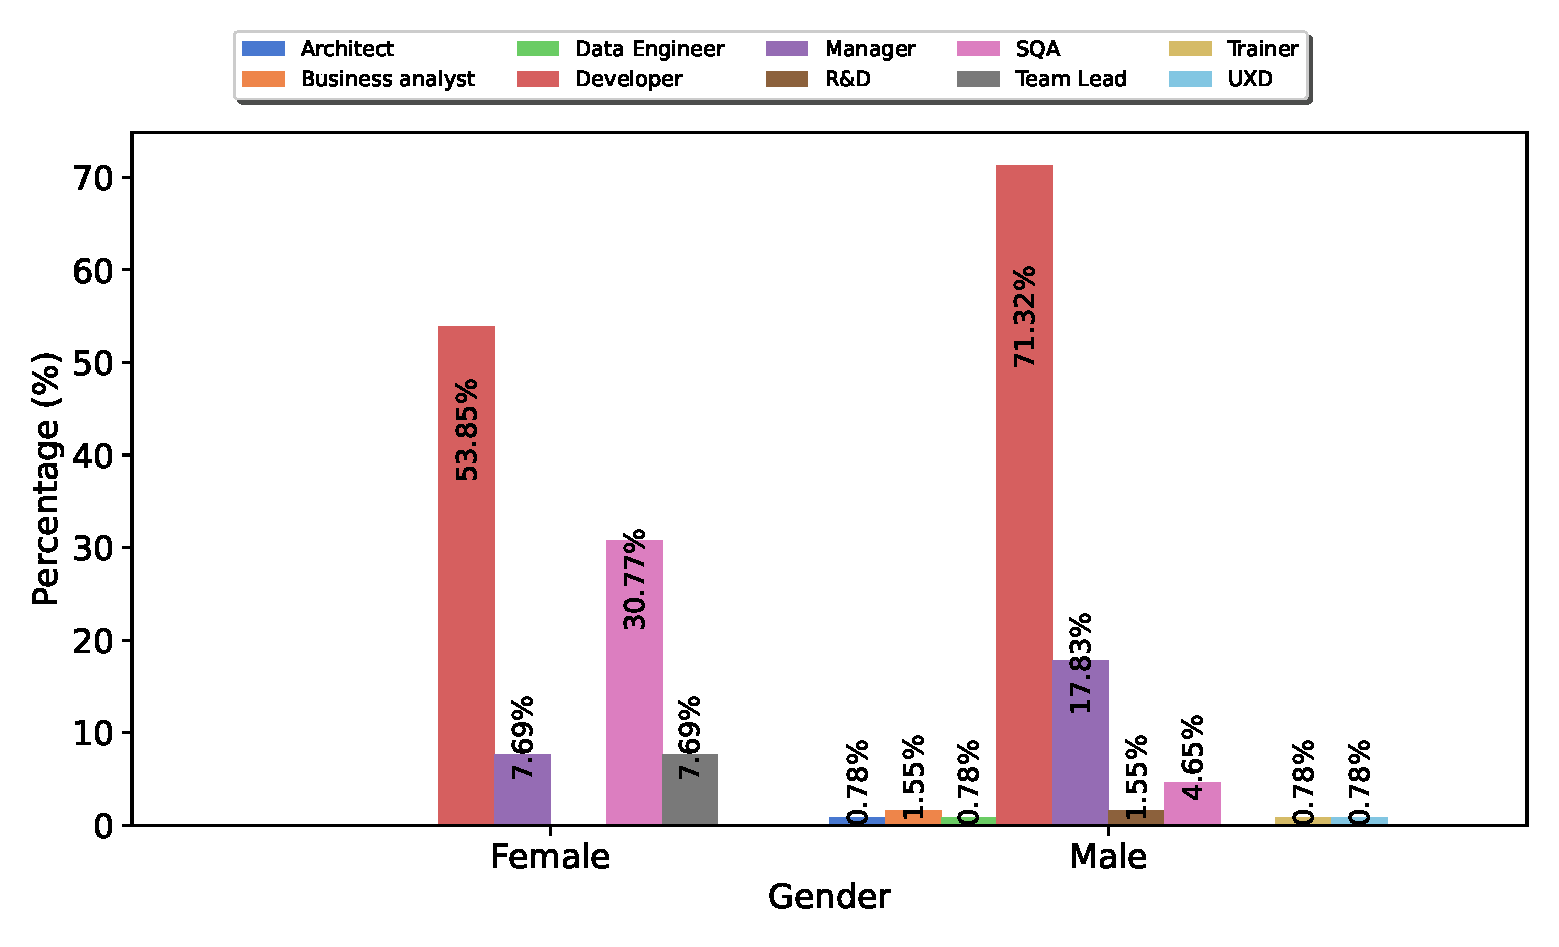
\includegraphics[scale=0.4]{Figures/Gender_and_Role}
 \caption{Gender based role}
 \label{fig:gender and role}
\end{figure}
In terms of roles, the proportion of developers among female participants is comparatively low than that of male participants. However, the scenario is the opposite of the manager and team lead role. Generally, the developer role is considered a junior role, and the manager/team lead is considered a senior role. Thus, it is clear from Figure \ref{fig:gender and role} that there is a difference between junior and senior roles among female participants. This indicates that in recent years females are less interested in joining the SE industry. Also, among ten different roles, female participants are holding only four types of roles. Our findings align with the survey result of Hussain et al.\cite{Hussain2020}. They found that female participants are only limited to developer, QA, and project manager roles, where male participants are holding varying types of roles in the Bangladesh SE industry. The result of the Stack Overflow survey\cite{StackoverflowSurvey2020} is slightly different. In the SO survey, female respondents are mostly data scientists, business analysts, QA, and developer roles. A common theme in all surveys is the role of female respondents in the QA.

\newcolumntype{b}{X}
\newcolumntype{v}{>{\hsize=.03\hsize}X}
\newcolumntype{m}{>{\hsize=.2\hsize}X}
\newcolumntype{y}{>{\hsize=.33\hsize}X}
\begin{table}[htbp]
    \centering
    \caption{Highlights of Findings from Survey Closed Questions by Gender}
    \begin{tabularx}{\textwidth}{v|b}
        \hline
        \textbf{No}     & \textbf{Question}  \\ \hline
        2 & What is your age?\newline
        1) 15 to 20: \textbf{\textit{Male, 100.0\% } } 2) 20 to 25: \textbf{\textit{Male, 87.8\% } } 3) 25 to 30: \textbf{\textit{Male, 86.84\% } } 4) 30 to 35: \textbf{\textit{Male, 96.0\% } } 5) 35 to 40: \textbf{\textit{Male, 100.0\% } } 6) 40 to 45: \textbf{\textit{Male, 100.0\% } } \\ \hline
        4 & For how many years have you coded professionally?\newline
        1) less than 2: \textbf{\textit{Male, 89.13\% } } 2) 2 to 5: \textbf{\textit{Male, 91.18\% } } 3) 5 to 10: \textbf{\textit{Male, 80.77\% } } 4) more than 10: \textbf{\textit{Male, 100.0\% } } \\ \hline
        5 & What is your current role?\newline
        1) Architect: \textbf{\textit{Male, 100.0\% } } 2) Business analyst: \textbf{\textit{Male, 100.0\% } } 3) Data Engineer: \textbf{\textit{Male, 100.0\% } } 4) Developer: \textbf{\textit{Male, 92.93\% } } 5) Manager: \textbf{\textit{Male, 95.83\% } } 6) R\&D: \textbf{\textit{Male, 100.0\% } } 7) SQA: \textbf{\textit{Male, 60.0\% } } 8) Team Lead: \textbf{\textit{Female, 100.0\% } } 9) Trainer: \textbf{\textit{Male, 100.0\% } } 10) UXD: \textbf{\textit{Male, 100.0\% } } \\ \hline
        6 & Which of the following software development methodologies do you follow?\newline
        1) Agile: \textbf{\textit{Male, 86.36\% } } 2) Kanban: \textbf{\textit{Male, 100.0\% } } 3) Others: \textbf{\textit{Male, 100.0\% } } 4) Pair Programming: \textbf{\textit{Male, 96.43\% } } 5) Scrum: \textbf{\textit{Male, 93.75\% } } 6) Waterfall: \textbf{\textit{Male, 100.0\% } } 7) XP: \textbf{\textit{Female, 100.0\% } } \\ \hline
        9 & Which of the following technologies do you have experience working in?\newline
        1) Cloud: \textbf{\textit{Male, 100.0\% } } 2) Desktop: \textbf{\textit{Male, 78.57\% } } 3) Embedded /IOT: \textbf{\textit{Male, 100.0\% } } 4) Mobile: \textbf{\textit{Male, 90.62\% } } 5) Others: \textbf{\textit{Male, 100.0\% } } 6) Web: \textbf{\textit{Male, 90.0\% } }\\ \hline
    \end{tabularx}
    \label{table:analysis by gender}
\end{table}

The interesting findings of gender analysis are presented in Table \ref{table: analysis by gender}. James et al.'s\cite{James2017} survey on male and female software professionals found that men are more likely to be in senior positions than women. In Q4 of Table \ref{table:analysis by gender}, we observe a similar scenario. However, in our case, the observation is not statistically significant. They also found that male software practitioners tend to be older than female practitioners and female practitioners tend to leave jobs in mid-career. We observe the same phenomena in Q2 and Q4, and the finding may be true in Bangladesh.


James et al.\cite{James2017} found that female practitioners express less satisfaction with the spirit of teamwork inside the organization. They conclude that this characteristic would make male practitioners a key part of a good agile team. Our findings differs from James et al. \cite{James2017}. In Q6 of Table \ref{table:analysis by gender}, we observe that our survey's female participants prefer the Agile methodology over other software development methodologies. However, development methodology selections are often performed by senior management. Thus, personal preferences can have minimal effect on this choice

In James et al.'s survey, neither male nor female was not dominating any particular technology field. However, in Q9 of 
Table \ref{table:analysis by gender} we observe female participants working on desktop, web, and mobile. As a small SE industry, cloud/IoT is considered a less secured field as job opportunities in these fields are small. It seems female participants tend to work in a more secure technology (in terms of a job opportunity) field.


\subsection{Analysis by Size}
\label{analysis by size}
We have presented the respondents' company size in Figure \ref{fig:company size}. It seems that our survey respondents are mainly from medium and small companies. We have compared our survey with the StackOverflow survey results from 2017 to 2020\cite{StackoverflowSurvey2017,StackoverflowSurvey2018,StackoverflowSurvey2019,StackoverflowSurvey2020}. In the SO survey, more than half of the respondents are from companies with employees ranging from 1 to 150. It seems small and medium-sized companies are the global trend in software industries.

\begin{figure}[h]
\centering
  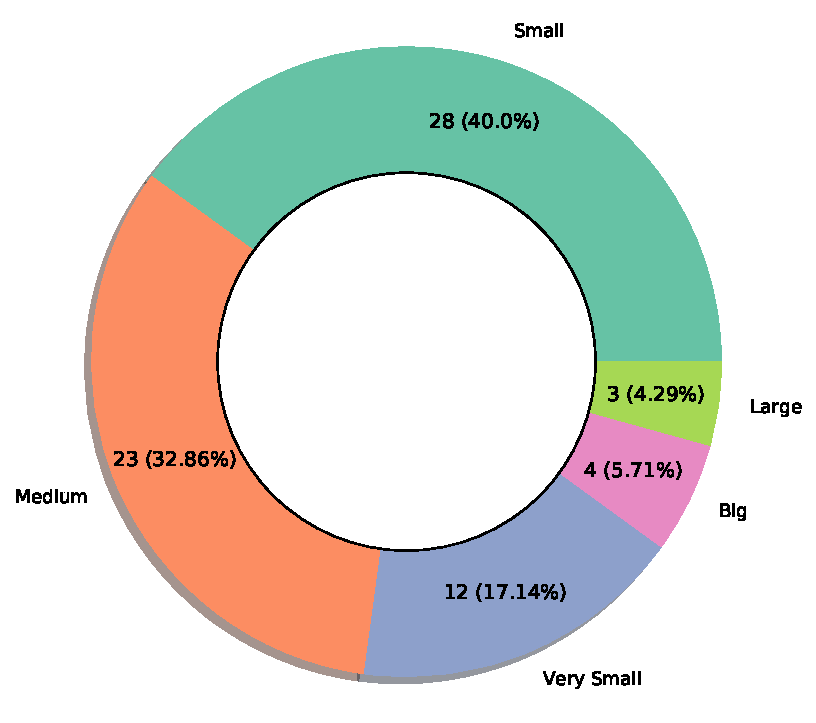
\includegraphics[scale=0.45]{Figures/Company_Size}
  \caption{Distribution of the size of respondents companies}
  \label{fig:company size}
\end{figure}

To get an idea of the companies' distribution of experience, we plotted the experience along with company size in Figure \ref{fig:experience and company size}. It is expected that companies will have a composition of different experience levels. However, we observe that big and large companies do not pose any composition of different experience levels. It is often seen that the senior position of big and large companies are often held by international candidates rather than a local candidate. However, we have too few respondents from big and large companies to draw any conclusion.

\begin{figure}[h]
\centering
  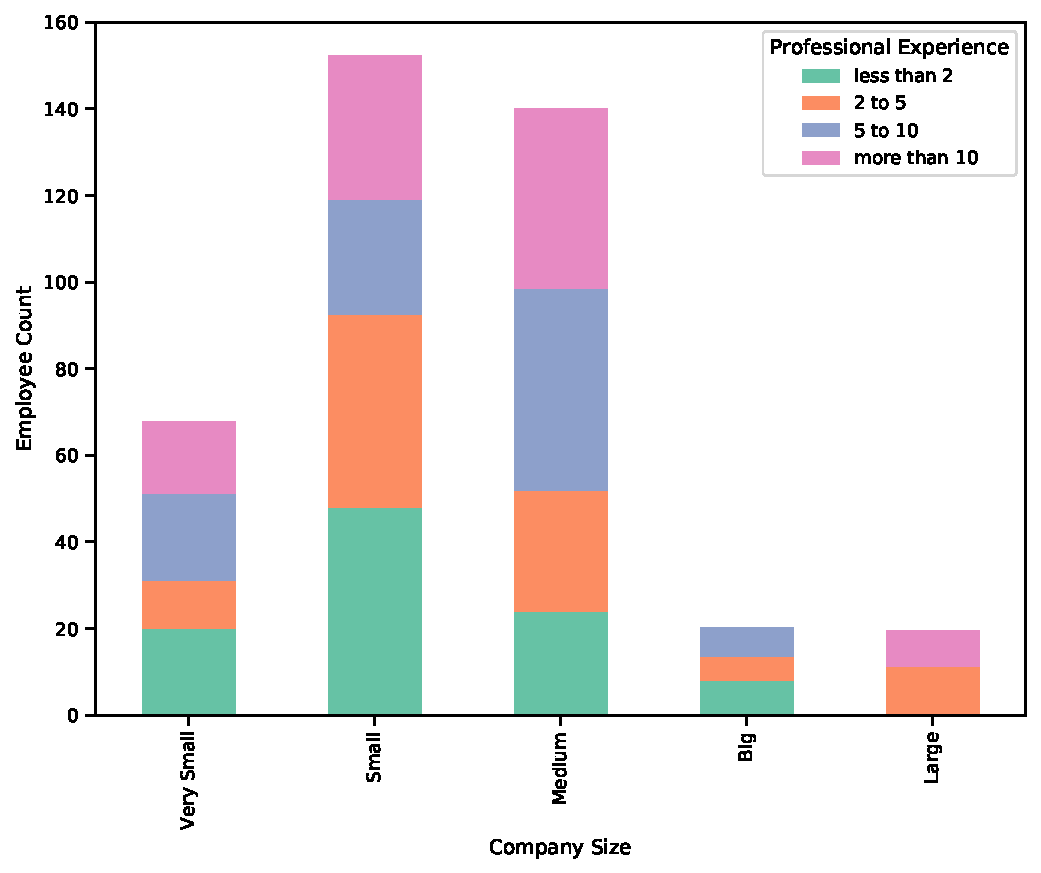
\includegraphics[scale=0.45]{Figures/Employee_Company_Size}
  \caption{Distribution of the experience}
  \label{fig:experience and company size}
\end{figure}

Testing practices are considered to be related to company culture, and it is believed large companies maintain better company culture than small companies. To check automatic testing practices among large and small companies, we plotted them together in Figure \ref{fig:auto tets level and company size}. It is clear from the Figure \ref{fig:auto tets level and company size} that the highest level of automatic testing is mostly done in medium-sized companies.

\begin{figure}[h]
\centering
  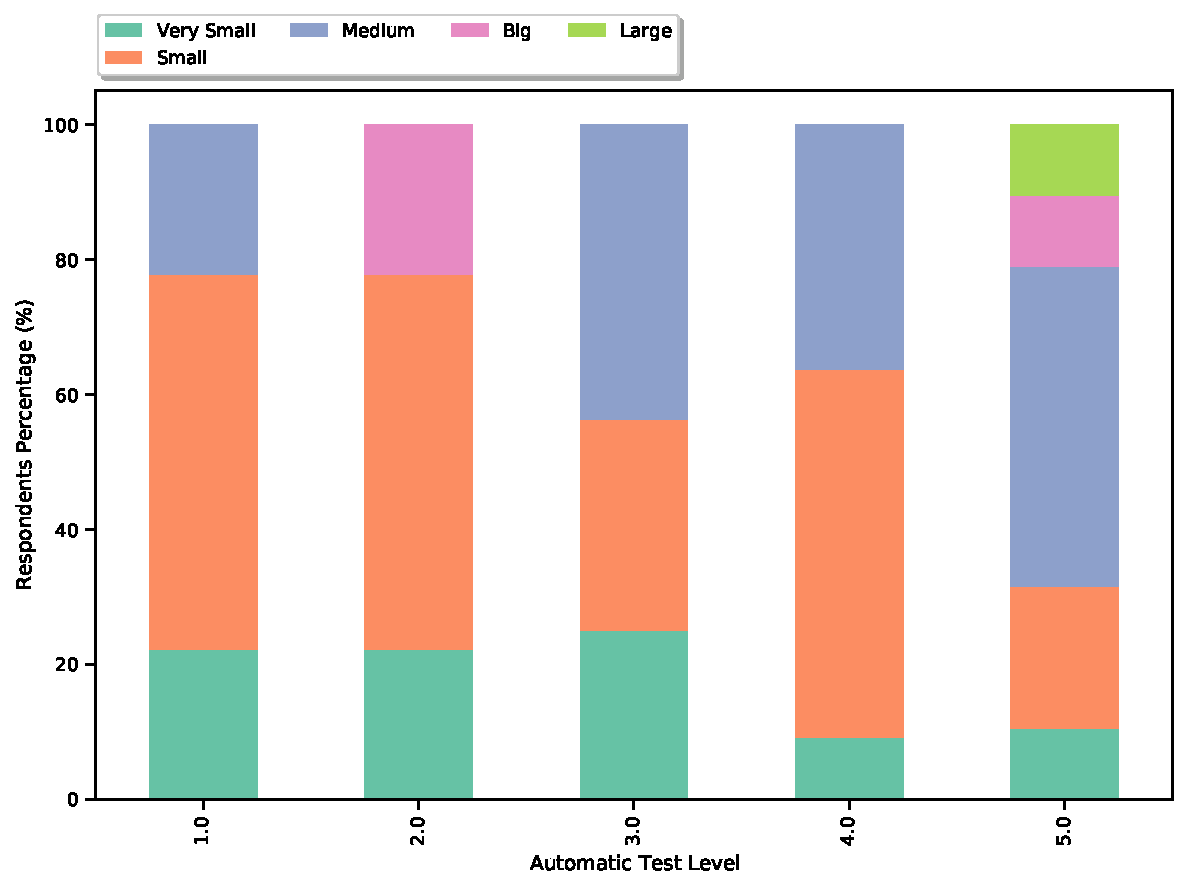
\includegraphics[scale=0.45]{Figures/Auto_Test_Company_Size.pdf}
  \caption{Automatic test level vs company size}
  \label{fig:auto tets level and company size}
\end{figure}

To understand how the technology stack is distributed among companies, we plotted the technology stack with company size in Figure \ref{fig:technology and company size}. It is clear from Figure \ref{fig:technology and company size} that comparatively newer technology is prevalent only in small and very small companies. One reason for such distribution can be that to survive in the competitive market, small and very small companies invested their time in newer technologies that are less practiced/ignored by large companies.

\begin{figure}[h]
\centering
  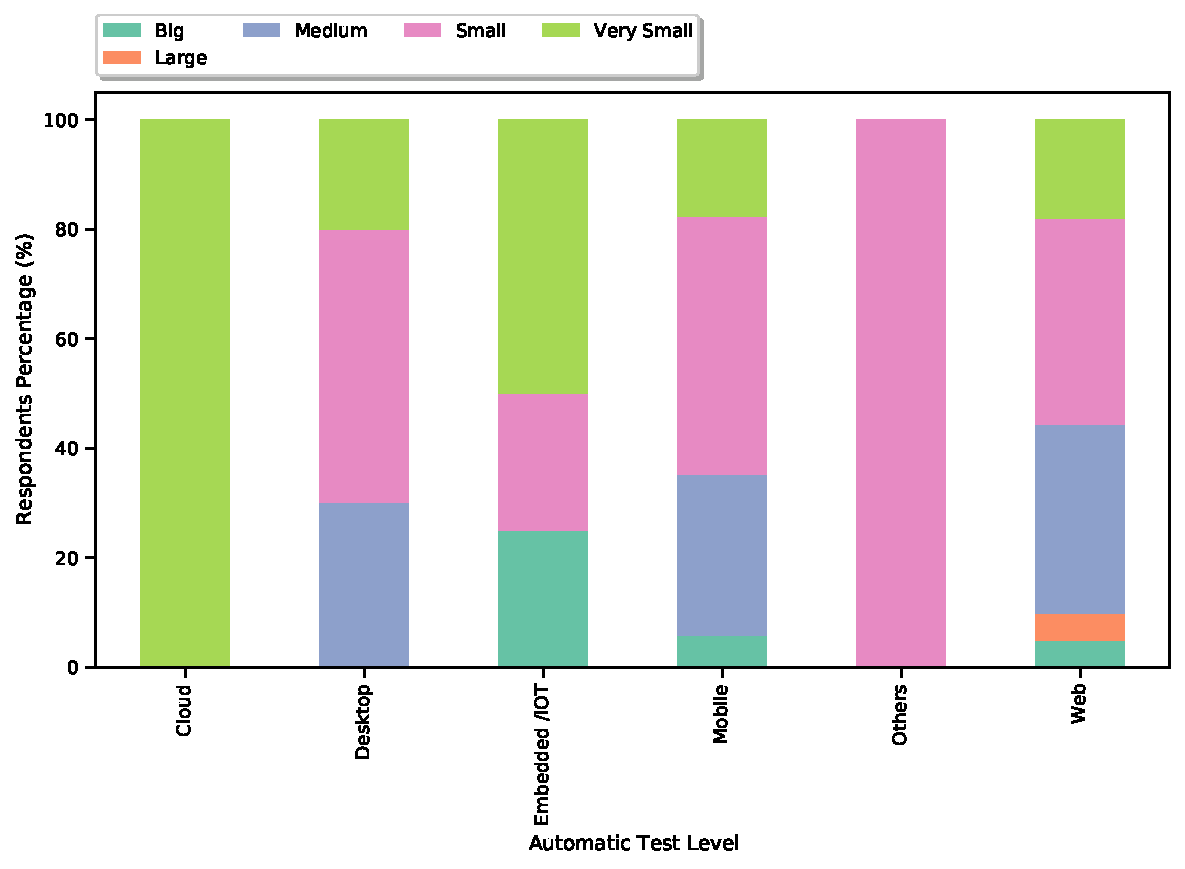
\includegraphics[scale=0.45]{Figures/Technology_Company_Size}
  \caption{Technology stack of companies}
  \label{fig:technology and company size}
\end{figure}

\section{Implications of Findings}\label{implications}
The findings from our study can guide the following major stakeholders in software engineering (SE): 
\begin{inparaenum}[(1)]
\item SE Tool Creators to develop usable and affordable automated testing framework that can be accessible to emerging countries,     
\item SE Researchers to compare and contrast software development practices in emerging countries with respect to region-specific and global trends,   
\item SE career enthusiasts who would like to participate in the high-growth software industries in the emerging countries,    
\item SE security and performance practitioners to develop techniques to better enforce such crucial non-functional requirements in software products in emerging countries, and  
\item SE Industry leaders to offer customized region-specific software products and to promote diversity irrespective of regions.   
\end{inparaenum} We discuss the implications below.
% what are the implications of findings? say for another emerging country or software professionals or companies like Microsoft, Google?

 

\bf{\ul{Tool Creators.}} We have found that rigorous testing practice
is not prevalent in Bangladesh. The difference in testing effort between the
established software industry (e.g., Canada) and Bangladesh is too high. The
scenario is also true for other developing countries like Pakistan. From our
study, software practitioners may have an idea of their standing in software QA
in testing. Similar to all emerging industries, security testing is less
prioritized in Bangladesh. From our comparison, developers may better understand
security testing and security practices in other countries. While these findings show a 
difference in the adoption of testing tools and non-functional measures 
between emerging and developed countries, the reasons could be multi-faceted. 
For example, one reason of the prevalence of less automated testing in emerging countries 
like Bangladesh is that most of the developed software products are web-based. This means 
that developers in Bangladesh need to test their GUI-based software product. 
Proper software testing tool support for GUI testing is in infancy compared to 
the testing of source code. Good GUI-based testing tools are also not 
free or open-source. This makes it hard for developers in emerging countries to 
learn and use GUI-based testing framework. Therefore, 
while unit testing is practiced widely in Bangladesh as like any other countries, 
the lack of automated testing is really due to the nature of the software products 
they developers are entitled to work on and the availability of good, usable and affordable 
testing framework to support them. Therefore, SE tool creators may create a
user-friendly framework to implement automatic testing for different types of
testing to address this affordability issue. Alternatively, 
cheaper and/or more affordable versions of the industry standard automated testing framework 
can be offered to developers of emerging countries. Containerization technologies are a popular trend worldwide. However, the
practice of containerization technologies is too low. Automatic
deployment/release is another under-practiced area. Tool creators can investigate
the challenges to incorporate these technologies in an emerging SE industry like
Bangladesh and offer more affordable alternatives. This is important because a software 
product developed in an emerging country like Bangladesh is actually consumed mostly in the developed 
countries (e.g., via outsourcing). Therefore, anyone can suffer from any lingering faults in the developed software products.

% Moreover, we have
% shown the level of automatic testing in the Bangladesh SE industry. Automatic
% testing is directly related to productivity. Practitioners can increase their
% productivity by implementing automatic testing for their products. Similarly, we
% have observed the under-use of automatic deployment/CI-CD tools. Practitioners
% should focus more on this area to automate their product pipelines.
% 
% We have also found that testing has been given less priority in the industry though
% it is one of the key elements for ensuring software quality. Furthermore,
% automatic testing, which is crucial for the efficiency and productivity of the
% test team, is rarely used. An automatic testing framework for other types of
% testing (such as GUI testing) may increase automatic testing practice. The price
% of quality automated testing tools may cause a lack of their use as the software
% budget in developing countries is often limited. Researchers 

\bf{\ul{Researchers.}} In SE research, we need to be aware of the current trends in software development practices not only 
to guide our research along the trends but also to ensure that our research contributions are timely and effective to the current 
needs of the software industry. In research, we strive to achieve generalizability of our findings, because otherwise we 
run the risk of becoming too niche or specific that may not cater to a global audience. Our study results of 
software development practices in an emerging country like Bangladesh and the comparison of 
such practices against multiple countries worldwide show that development practices, tools, techniques all could 
vary across the countries. Therefore, it may not be always possible to observe or enforce 
similar development practices across the globe, even when certain practices may be perceived as superior to others. 
A major reason of the observed differences between the emerging 
countries and developed countries is that outsourcing is a still a major source of revenue 
for the software industries in emerging countries. This explains why product design and overall architecture design 
is not widely practised in the software industries of emerging countries. A major 
focus in software engineering research is to understand team cohesion and collaboration. Given 
the outsourcing nature of the works carried by the software companies in the emerging countries, 
we can expect that the developers in the companies need to adapt to constantly dynamic teams where some 
team members are local and some others are remote and temporary, e.g., members from a software company 
of a developed country that are engaged in the outsourcing work. It is important to understand 
the productivity of the developers in such dynamic environment, the 
challenges they face (e.g., lack of enough in-person communication due to remote work and time difference).
Such research can offer findings in the development new methodologies, tools and techniques to facilitate 
better communication and collaboration practices among the developers in the such teams. This can 
then also help the software companies in emerging countries to offer better support to the overall system 
design and planning. 

\bf{\ul{Career Enthusiasts.}} We have found that certain languages (e.g.,
Java, JavaScript, etc.) and frameworks (e.g., Spring, Django, ASP.NET) have
extensive use in the software industry of Bangladesh. This finding is not different from 
other emerging countries. Therefore, career enthusiasts who aspire for a software development profession in 
emerging countries may focus on mastering such skills. Universities can update
their curricula to meet industry demand. The students aspiring to join the
software industry must prepare themselves accordingly to be productive quickly.
We have also found less automated testing practices in the industry of
Bangladesh. This may be related to a lack of exposure to the testing framework.
Similar to Hussain et al.\citep{Hussain2020}, we also suggest including
testing-related courses into the curriculum of universities and introducing
relevant assignments to have hands-on experience on automated testing tools
right from the student level. The students in their academic projects should
also use container and other DevOps tools to bring some qualitative improvement
for the industry when they join there.

\bf{\ul{Security and Performance Practitioners.}} More than 9.5\% of our respondents
responded that they do not take any measures to mitigate the security risk. The
common reason for not taking any measures is (1) the product is an early stage
(2) the respondents' role does not require any product security measures. The
reason for not taking any security measures is different from North
America \citep{Assal2019}. The reasons are (1) there are no formal test plans,
(2) lack of knowledge regarding testing tools. Though respondents do not think
about product security initially, it is recommended \citep{Chandra2009,Azham2011}
to plan security tests and product security from the design phase.

Modern frameworks provide the basic security of the solution. Moreover, some
framework provides enhanced, focused, customized security through a plug-in or
add-on, e.g., spring-security, spring-cloud security. Framework-based security
is a growing practice in the software industry\citep{Alssir2012}. The practice
in the Bangladesh SE industry matches the global practice. According to our
survey, it is the second most popular measure to mitigate security risk. Survey
respondents have reported using OWASP, HDIV, and spring security. Srinivasan et
al.\citep{Srinivasan2017} have conducted a comparison among the popular web
frameworks based on security. Based on five criteria, they ranked the
frameworks, and all of the mentioned frameworks of our respondents are in the
top 10 list. It seems that secure software engineering practice is prevalent in
the Bangladesh SE industry.


On a survey of 237 software professionals, Elahi et al.\citep{Elahi2011} found
that 51\% of respondents maintain at least one security standard, and 19\% of
respondents maintain ISO 17799 security standard. On the contrary, about 29.63\%
of respondents of the Bangladesh software industry maintain any security
standard. It is clear that security standards are not that much popular in this
SE industry.

According to Smith et al.\citep{Smith2003}, efficient architecture and
continuous monitoring tools are two of the twenty-four best practices to ensure
software performance. The respondents report both practices. However, Smith et
al. presented twenty-one other best practices, and we have not found other
practices in our survey. It is clear the SE industry of Bangladesh only
practices a few best measures for ensuring software performance.

% 27.1\% of respondents in our survey reported that they use the load balancer
% to ensure software performance. A load balancer is mostly used to reduce queue
% time/ response time in web base application\citep{Mesbahi2016}. Thus we can
% infer that most of our survey respondents mainly engaged in developing the
% web-based application.


Bondi et al.\citep{Bondi2000} have listed four scalability types to ensure
software capability to scale; however, we observe only one scalability type
(load scalability) in our responses. To obtain software scalability use of cloud
services is one of the most popular strategies\citep{Gao2011}. Another popular
strategy is the use of microservice. Microservice and cloud services together
allow the user to scale up and down any system dynamically. C\'{a}ceres et
al.\citep{Cceres2010} reported that cloud services and microservice-based
architecture are generally used together to ensure scalability. In the
Bangladesh SE industry, this practice may be prevalent. The use of cloud service
and efficient use of architecture are the second and third most popular topic
among our respondents.

Overall, the findings show that much need to be done to ensure proper security and performance measures 
in the software development practices of emerging countries. Multi-faceted efforts are warranted like 
development of affordable tools and techniques for the emerging countries, enforcement of widely-accepted and 
measurable industry standards across the regions, and the proper training of the security and performance 
principles to the developers in emerging countries. 

\bf{\ul{Industry Leaders.}} This study found that the Bangladesh software
industry lags in adopting some of the current industry trends. Bangladesh can be
a good marketplace for cloud companies like Microsoft, Google, and Amazon if
they provide an affordable package for the software companies operating here.
Local entrepreneurs may also think of building cost-effective local public
clouds along with providing some common DevOps services.

Moreover, we have found most of the participants in our study are engaged in web
technology. This may indicate that the web is the most popular form among users
of Bangladesh. This observation can help the industry owners to select
appropriate medium while targeting users of this region. %We have identified
common practices of the practitioners of the Bangladesh software industry.

Finally, we have identified that the
participation of female in the Bangladesh SE industry is comparatively less than
that of male engineers (see Section \ref{analysis by gender}). Hussain et al.\citep{Hussain2020} expressed a
concern that there may be bias in the hiring process of the industry. Overall, the under-representation of 
females and minorities in software industries worldwide is a prevalent and ongoing concern. 
This was also reported in the 2020 Stack Overflow developer survey, where more than 90\% respondents 
were males. Our findings confirm similar trends in Bangladesh. Therefore, proper measures 
need to be taken to encourage equity, diversity, and inclusion in software industries across the regions.  
Such measures may be better enforced by tailoring the measures to region-specific cultural attributes.
%Further
%research may be conducted to identify the inherent reason behind these facts.


\section{Threats to Validity}
\label{validity}

\subsection{Construct Validity}
% Construct validity threats concern the relation between theory and
% observations. 
Construct validity is mainly concerned with the extent to which the
study objectives truly represent the theory behind the study\cite{Wohlin2012}. In our study, we have used open coding strategy to label the survey responses. The nature of this coding strategy may introduce researcher bias into coded labels. To mitigate the issue, the labels have been coded by two individuals, and the codes are accepted when there is a reasonable agreement among the coders. Another issue can be whether our data actually represents real-world SE practices. This study counted the votes and made statistical inference, which is common in survey-based studies. It is believed that voting data can, to a certain extent, reflect the opinions of the majority. It was previously observed\cite{Garousi2015} \anindya {where observed? cite?}\partha{added} that people tend to form their answers close to expected answers when evaluated. To mitigate the threat, before the survey, we informed participants that our motive in this survey was to get a decent understanding of current practices, and we do not intend to collect any personally identifiable data. Construct threats may also be introduced by a misleading interpretation of the survey questions. We conducted a preliminary survey and interview session with some participants to rule out any ambiguity from survey questions and thus tried to reduce such risk.

\subsection{Internal Validity}
% Threats to internal validity refer to how well the research is
% conducted.
Internal validity is a property of scientific studies that refers to how well a study has been conducted. A threat to internal validity in this study is inherent in the participant selection bias. We used several social platforms, personal connections to reach as many participants as possible. Another threat could arise from the placement of the options in a multiple-choice question. It is often observed that survey participants often show bias towards the first option in any multiple-choice question\cite{Uddin2019} \anindya{Can you cite?}\partha{added}. However, in one of the multiple-choice questions (Q9), the `Web' option was placed at the bottom of the list. Despite this placement, we observed most of the participants selected `Web' as a technology platform. But practically, from the personal experience of the authors, there is no bias in this opinion.


\subsection{External Validity}
% Threats to external validity compromise the confidence in stating
% whether the study results apply to other groups.
External validity is concerned with the generalization of the study result. In our study, we have participants from almost all the groups of the Bangladesh software industry. However, it is difficult to claim the statistical generalizability of our findings, given that our sample included 137 respondents where there 1100+ companies and 3,00,000 IT professionals\cite{BASIS2018} in the software industry of Bangladesh \anindya{make it consistent with intro.}\partha{updated}. Moreover, emerging IT industries share a common trend of challenges\cite{Sison2006, lloyd2020}. Thus, our findings are also applicable to other emerging software industries across the globe.
\section{Conclusion}
\label{sec:conclusion}
Thanks to the results of this survey, we have observed that software industry in Bangladesh is
spirited, growing and competitive that many software teams are eager for adopting state-of-theart software engineering practices and approaches.Awareness and knowledge about these practices and approaches are rising in the industry, that many organizations have been establishing
them within their development operations. We have also observed that the industry needs to
improve on using well-established requirements engineering and testing related practices.These
two areas are where most displeasure is stated about. Also we observed that practitioners have
a tendency to avoid formal or relatively complex best practices (e.g.TDD, formal languages,
pair programming, automation testing and metric usage) in general, but especially in these two
areas. We suggest organizations to invest in improvement and training efforts for increasing
the awareness and knowledge about these software disciplines.In this study, we have seen that
social aspects are important as well that many practitioners have expressed their discontent and
difficulties on issues like communication, collaboration, and team structure.



%\section{Introduction}
\label{introduction}

%The software engineering (SE) industry in Bangladesh is considered relatively small compared to the size of its population (160 million-plus) and the size of the national economy. %Yet, the software industry in this country has started rapidly emerging and become part of Bangladesh's rapid development in recent years. 
%The majority of software companies were established after 2000 and have become a crucial resource for the economy of Bangladesh \cite{Basis2017}, and also the growth rate is expected to continue sharply. This propitious growth is bolstered by export trends and a large demand for IT automation in the domestic market. To continue this achievement by fulfilling the growing expectations of software consumers, the SE industry needs to follow standard practices in producing good quality software products. %Thus for this, we have to first point out how the software development process is exercised in such a rapidly emerging industry. 

%The practice of software development varies from region to region. A certain methodology may become more efficient in some regions but is not considered efficient in other regions. Although most of the factors behind software development are the same all the time, there are certain points that vary from region to region. For software development professionals, deciding on processes, practices, and techniques is critical. Sometimes, these decisions might be based on marketing and literature bias that supports the new or industry-supported practice.

%Many studies concerning the practices of software development have been conducted. Those studies convey similarities, but also differences in diverse regions, countries, and communities. Previous empirical studies have gone into how software development practices were conducted in North America, Europe, Turkey, New Zealand, etc. There are some prior studies on the Bangladesh software engineering (SE) industry, but the studies' focus and dimension were different. To the best of our knowledge, this is the first study to identify software engineering practices in emerging countries by taking the software industry in Bangladesh as a case study on how the software industry in an emerging environment works, the challenges they face, and the practices they adopt.

The software industry of a developed country differs from that of a developing country in many aspects. Easy migration opportunities of the developers cause constant scarcity of experienced people in developing countries. Still, due to the abundance of Computer Science graduates, the software industry of some developing countries are continuing to emerge by catering to the majority of the local market as well as expanding in the global market with reasonable price. Bangladesh is such a country with a rapidly growing economy and a 160 million population. IT sector is considered a priority sector in Bangladesh over the last decade. The software development industry dominates this sector by providing the majority of local needs and exporting abroad. According to the Bangladesh Association of Software and Information Services (BASIS), 1100+ software companies operate in Bangladesh, where around 40\% have a global business. The foreign revenue earned by the industry is over 800 Million USD~\cite{BASIS2018}. 

A study on the software development practice in the industry of a country reveals the challenges and scopes of improvement for that industry as well as for industries of similar types. There are several studies on the software industry of countries with established reputation as a software manufacturer. However, the issues and characteristic of an emerging software industry varies greatly from those countries. In this research, we focus on the picture of such industries and selected Bangladesh as a representative of this category. Bangladesh has to compete with neighboring countries of similar socio-economic backgrounds such as India, Pakistan, Sri Lanka, etc. They are likely to share similar shortcomings and strengths. Hence, this study may help to understand the nature of the industry in these countries as well.

%Computer Science and Engineering (CSE) is the most demanding subject choice among the best students in the country. The strength of Bangladesh in this area has been manifested by continuous success in flagship competition ACM International Collegiate Programming Contest (ICPC) for the last two decades. Also, the software engineers from Bangladesh work in almost all the leading software companies of the world. 

 The delivery of quality outcomes on time with a competitive budget is a major challenge for the software industry. The practice of state-of-the-art SE methods and technologies is indispensable to achieve success. The purpose of this research is to systematically study and characterize the Software Engineering (SE) practices in Bangladesh, i.e., the tools and technology used for design, development, testing, and deployment. Similar studies were carried out in other countries such as Canada, Turkey, Netherlands, and New Zealand to have a mature understanding of the gap between SE research and actual practice in the industry~\cite{Garousi2013, Garousi2015, Vonken2012, Wang2018}. The current study also presents a comparative picture of SE practices in Bangladesh and other countries. 

For a software development company, the choice of technology evolves over time and varies widely according to application type. This study is likely to benefit different stakeholders such as potential local and global clients, students, i.e., future practitioners, etc. by presenting relevant industry practice. Another major benefit of such a study is having insight into different dimensions of industrial practice that help design better curriculum for current students and reveal the need for continuous education components for existing practitioners. We also aim to figure out both similarities and dissimilarities in the development practices of Bangladesh with other countries, which would eventually reveal the areas where this industry needs improvement.

This study aims to consider detailed activities beyond high-level practices gathered through surveying individual professionals. The survey was conducted in two phases, a limited primary survey with selected respondents and a final survey. The goal of the primary survey was to find any discrepancy or ambiguity in the survey questions. Also, the primary survey had an interview session with each respondent. From the findings of the interviews, the question of the survey was later adjusted. The survey is designed to reveal the methodology of software development practices, the adoption of technologies and tools by the professionals, and the use of testing and deployment practices in the company where the individual concerned works.  
\anindya{The two stages of the survey (manual interview and online), involvement of management - these may be discussed briefly.}\partha{Added}

%\anindya{Gias bhai suggests that we should say that we have 2 research questions. We explore these two from 4 dimensions. In this way we can make the following discussion more precise.}

%More specifically, we answer the following research questions around the two studies:
%We studied from two perspectives: (1) Understanding development practices in Bangladesh: We aim to perceive what methodologies, technologies, and testing practices are followed in software companies. (2) Comparison among the countries: We aim to figure out both similarities and dissimilarities in the development practices of Bangladesh with other countries, which would eventually reveal the areas where this industry needs improvement.
We want to explore two research questions in this study:

\begin{itemize}[leftmargin=10pt]
 
 \item \textbf{What are the major characteristics of software development practices and methods in Bangladesh?}
    
 \item \textbf{What are the similarities and differences in software development practices between Bangladesh and other countries?}

\end{itemize}

We explore these research questions from the following 4 dimensions.

\begin{itemize}[leftmargin=10pt]

    \item \textbf{What software methodologies are used in your project?}
    
    We investigate the development approaches and methodologies, requirements analysis processes, etc. It helps us to analyze the dominant practice of the industry and found that the software companies mostly follow the agile development model. In comparison with the other countries, it is found that Bangladeshi software companies generally spend significant time on the implementation stage of the development whereas technologically advanced countries spend more on system design and planning.
        
    \item \textbf{Which implementation technologies and tools are adopted by software development professionals?}
        
    This is to find out the current trending technologies like technology platforms, programming languages, frameworks, etc., in the software industries of Bangladesh that may help one who wants to pursue his career here. We have found that web-based software services are prevalent in the market and JavaScript is mostly used language for web development. The degree of use of different technologies and tools usually vary from country to country due to the availability of experienced developers, budget, etc. Hence, we are interested to explore if the companies in Bangladesh deviate from world standards for particular application domains.

%\anindya{One line result summery is there for last 2 RQs. For consistency, something should be mentioned for the first two as well.}\khalid{added}        
        
    \item \textbf{What type of testing and deployment practices are used?}
        
    We want to explore the present situation of testing and deployment practices adopted by the software firms in Bangladesh by investigating testing and deployment tools, test automation level, version control system, etc. This investigation enables us to find out if there is a need for improvement in these areas. We have observed that using test automation and deployment tools is not widespread in the industry, but there is scope of improvement in others. We also see that compared to developed countries, the test automation tool adoption is inadequate. This finding is expected to motivate practitioners to use automated tools for testing.
        
    \item \textbf{How are the security and performance ensured in a product of a company?}
        
    We try to understand how software companies secure and maintain their code and what practices are followed to ensure performance and scalability. The responses show that standards are followed for security assurance, tools are used for performance testing, and scalability is mostly ensured by using cloud services. In the comparative analysis with the reputed industry, the companies in Bangladesh lags behind in the area of automated performance testing and containerization that might ensure resource-optimized scalability.     
   
    %\item \textbf{What software methodology are used in your project?}
    
  %  \anindya{The above two comments do not make much sense to me. Please rephrase.}\khalid{updated}
    
 %   \item \textbf{Which implementation technologies and tools are adopted by software development professionals?}
     %   \item \textbf{What types of testing and deployment practices are used?}
    
    %\item \textbf{How are the security and performance ensured in the products of a company?}
    
\end{itemize}

Our findings show that the software companies in Bangladesh usually spend most of the time on the implementation stage rather than system design and requirement analysis. Also, the use of automated testing and tools for automatic deployment is quite low though nowadays, it is an integral part of a better and standard software development practice across the globe. Besides, we compare the development processes of Bangladesh with other countries and analyze them from several perspectives. These findings can help both managers and researchers to improve development practices in Bangladesh. On top of that, our study identifies the popularity of using cloud services, which may advise cloud companies to spread their market more than ever in Bangladesh or encourage private cloud development locally. Furthermore, our study presents the technologies and tools currently being used in Bangladesh's software firms that may help current students prepare themselves better for the industry.

\noindent\textbf{Paper Organization.} The remainder of the paper is organized as follows. Section~\ref{related_works} presents the related work to our study. Section~\ref{study_setup} describes the background of our study and the data collection procedure. Section~\ref{study_results} reports research questions about software development practices. Section~\ref{discussions} reports challenges and opportunities as well as analysis by several dimensions of software development practices. Section~\ref{implications} discusses the implications of our findings. Section~\ref{validity} discusses the threats to validity. Section~\ref{conclusion} concludes the paper.

%\section{Related Works}
\label{related_works}
\subsection{Studies of Development Practices and Processes}
\label{dev practice study}
In a study, Cusumano et al.\cite{Cusumano2003} have conducted a global survey on a completed software engineering project to identify software engineering practices. They have found that detailed architectural design and documentation is a common practice worldwide except the USA. In the USA, only 32\% of projects used detailed design specifications. One of the interesting findings of their study is the completeness of design before coding negatively correlates with the number of defects.

AlSubaihin et al.\cite{AlSubaihin2019} has identified the influence of the app store on software engineering practices. They have found that the perception of quality is slightly different among app store developers. App Store developers gave more priority to user rating than the traditional metrics like code quality and documentation when measuring software quality.

To identify the state of the practices in start-up companies, Klotins et al.\cite{Klotins2018} has conducted a study on start-up companies. They found that start-ups apply market-driven requirements engineering instead of the standard software engineering requirement engineering. However,  the applied requirements engineering practices are often rudimentary and lack alignment with other knowledge areas (such as design).

\subsection{Related Region-specific Studies}
\label{region specific study}

In 2012, Vonken et al.\cite{Vonken2012} surveyed Dutch software producing organizations to determine whether there is a gap between the current state of the practice and state of the art in software engineering. From 99 respondents, they extracted 22 interesting observations. These observations mark insights into the development process that they found unusual or surprising, at least from an academic perspective. This unusualness could either stem from certain principles being applied less or more frequently than expected or from unexpected correlations observed between factors.

The survey conducted by Garousi et al.\cite{Garousi2015} studies Turkey's software practices to characterize and understand the state of its SE practices. The military and defense software sectors are quite prominent in Turkey, especially in the capital Ankara region, and many SE practitioners work for those companies. 54\% of the participants reported not using any software size measurement methods, while 33\% mentioned that they had measured lines of code (LOC). In terms of effort, after the development phase(on average, 31\% of overall project effort), software testing, requirements, design, and maintenance phases come next and have similar average values (14\%, 12\%,12\%, and 11\% respectively). Respondents experience the most challenge in the requirements phase. As a rather old but still widely used life-cycle model, the waterfall is the model that more than half of the respondents (53\%) use. The next most preferred life-cycle models are incremental and Agile/lean development models with 38\% and 34\% usage rates, respectively. The Waterfall and Agile methodologies have slight negative correlations, denoting that if one is used in a company, the other will less likely to be used


A recent survey conducted by Wang et. al.\cite{Wang2018} in 2018 shows that, New Zealand professionals use similar methodologies as professionals in other countries. Key findings of their study are, (1) popular programming language in New Zealand software industry does not match with the worldwide ranking of popular languages (2) most of the time in SDLC is spent on implementation-related activities rather than  analysis and design.

In another study, Groves et al.\cite{Groves2000} reported that the New Zealand software industry pays particular attention to requirements gathering. They surveyed a selection of software companies with a general questionnaire and then conducted in-depth interviews with four companies. They found a clear difference in the testing phase between large and small software companies. Their finding is larger companies pay more attention to testing than smaller companies.

The study conducted by Sison et al.\cite{Sison2006} presents exploratory survey and case study results on software practices of some software firms in five ASEAN countries (Malaysia, Philippines, Singapore, Thailand, and Vietnam). They found that most of the forms in that region do not follow the standard procedure for SQA.

In a study focusing on the test practices in Canadian firms, Garousi et al.\cite{Garousi2013} found that the number of passing user acceptance tests and the number of defects found per day are considered the most important quality assurance metrics in Canadian firms. They compared their result to a previous study and showed that Canadian firms are giving more importance to testing related training than in the past.

Baharom et al.\cite{Baharom2006} had conducted a study on Malaysian software firms to find the effectiveness of standard practices. They found that alpha and beta testing was hardly implemented in software firms. Another interesting finding of their study is that most Malaysian firms emphasize implementation; only a  negligible number of companies spend more than 20\% of the effort in planning and design.

Zafar et al.\cite{Zafar2018} have surveyed why Pakistani software firms do not follow the standard requirement engineering process. They have found multiple issues contributing to the issue, such as lack of budget, lack of time, lack of dedicated team. However, the most prevalent issue is lack of budget; more than 60\% of their respondents have responded that the standard requirement engineering process was not followed due to scarcity of budget.

Based on a 200 participants survey, Hussain et al.\cite{Hussain2020} concluded that Bangladesh's computer science undergraduate education system leaves most of its graduates unprepared for the software industry. They suggested that updating the syllabus as part of the curriculum and including internships could help make graduates fit for the industry.

To identify the software engineering practices in Bangladesh, Rahim et al.\cite{Rahim2017} have surveyed 41 practitioners in the Bangladesh software industry. One of their interesting findings is the waterfall model holds the third position in terms of the popularity of SDLC models. They found that respondents found the Waterfall model risky for effective software development because more than 40\% of respondents indicated that requirement analysis and prioritization are the most challenging task in the software development process. In another survey focusing on testing practices in the Bangladesh software industry, Bhuiyan et al.\cite{M2018} found that most companies do not follow any standard SQA techniques for their projects. The interesting fact is such malpractice does not hinder their progress; in fact, they reported that these firms are in the industry for 6.5 years on average. However, in another survey Begum et al.\cite{Begum2009}  found that 47.5\% of respondents follow standard SQA techniques in their projects.
% \input{Sections/ResearchSetting}
% \input{Sections/Methodology}
%\section{Demographic}
\label{demographic}

\subsection{Respondent's Age}
Age of a person often determines his/her knowledge and experience with the focus of the survey. When administering a survey about SE industries, a respondent in his 24s and 25s will most likely answer the question differently than a respondent his 35s. The age distribution of our survey respondents is shown in \cref{fig:age}.
\begin{figure}[H]
\centering
  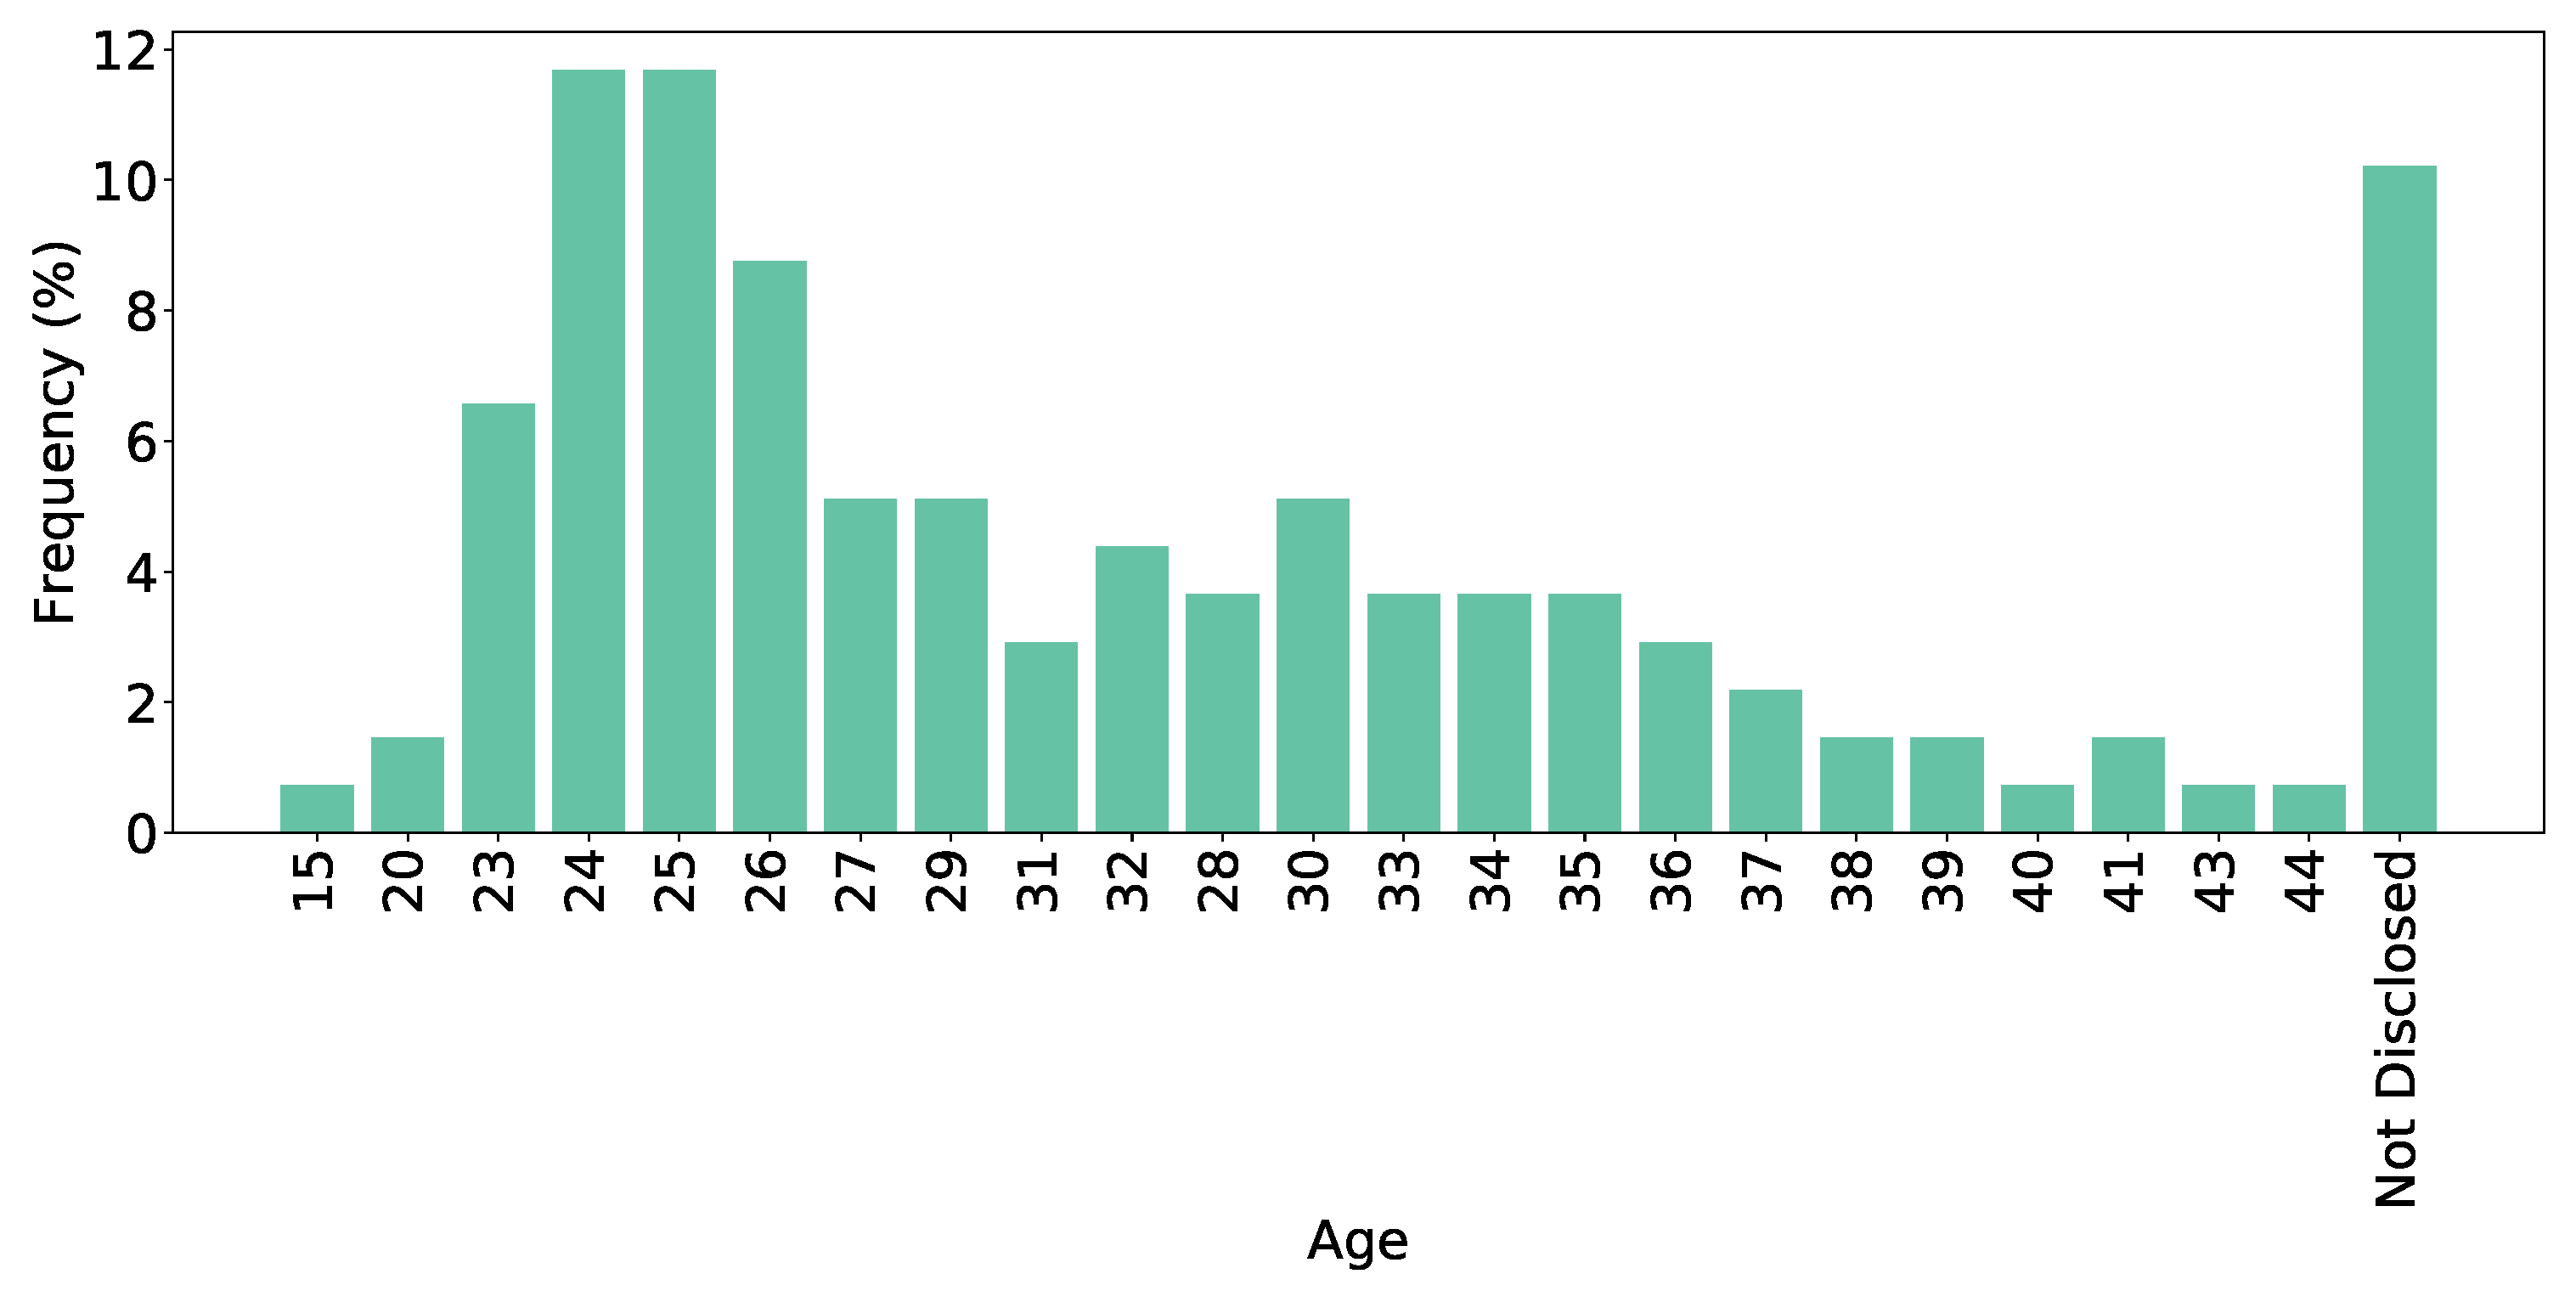
\includegraphics[width=0.8\textwidth]{Figures/Respondents_Age}
  \caption{Respondent's Age}
  \label{fig:age}
\end{figure}

\subsection{Work Experience}
Around 34\% of our respondent's has less than 2 years software development experiences. As the \cref{fig:experience} shows, we have respondent's with various years of work experience which will have positive impact by accumulating valuable results from wider audience base.
\begin{figure}[H]
\centering
  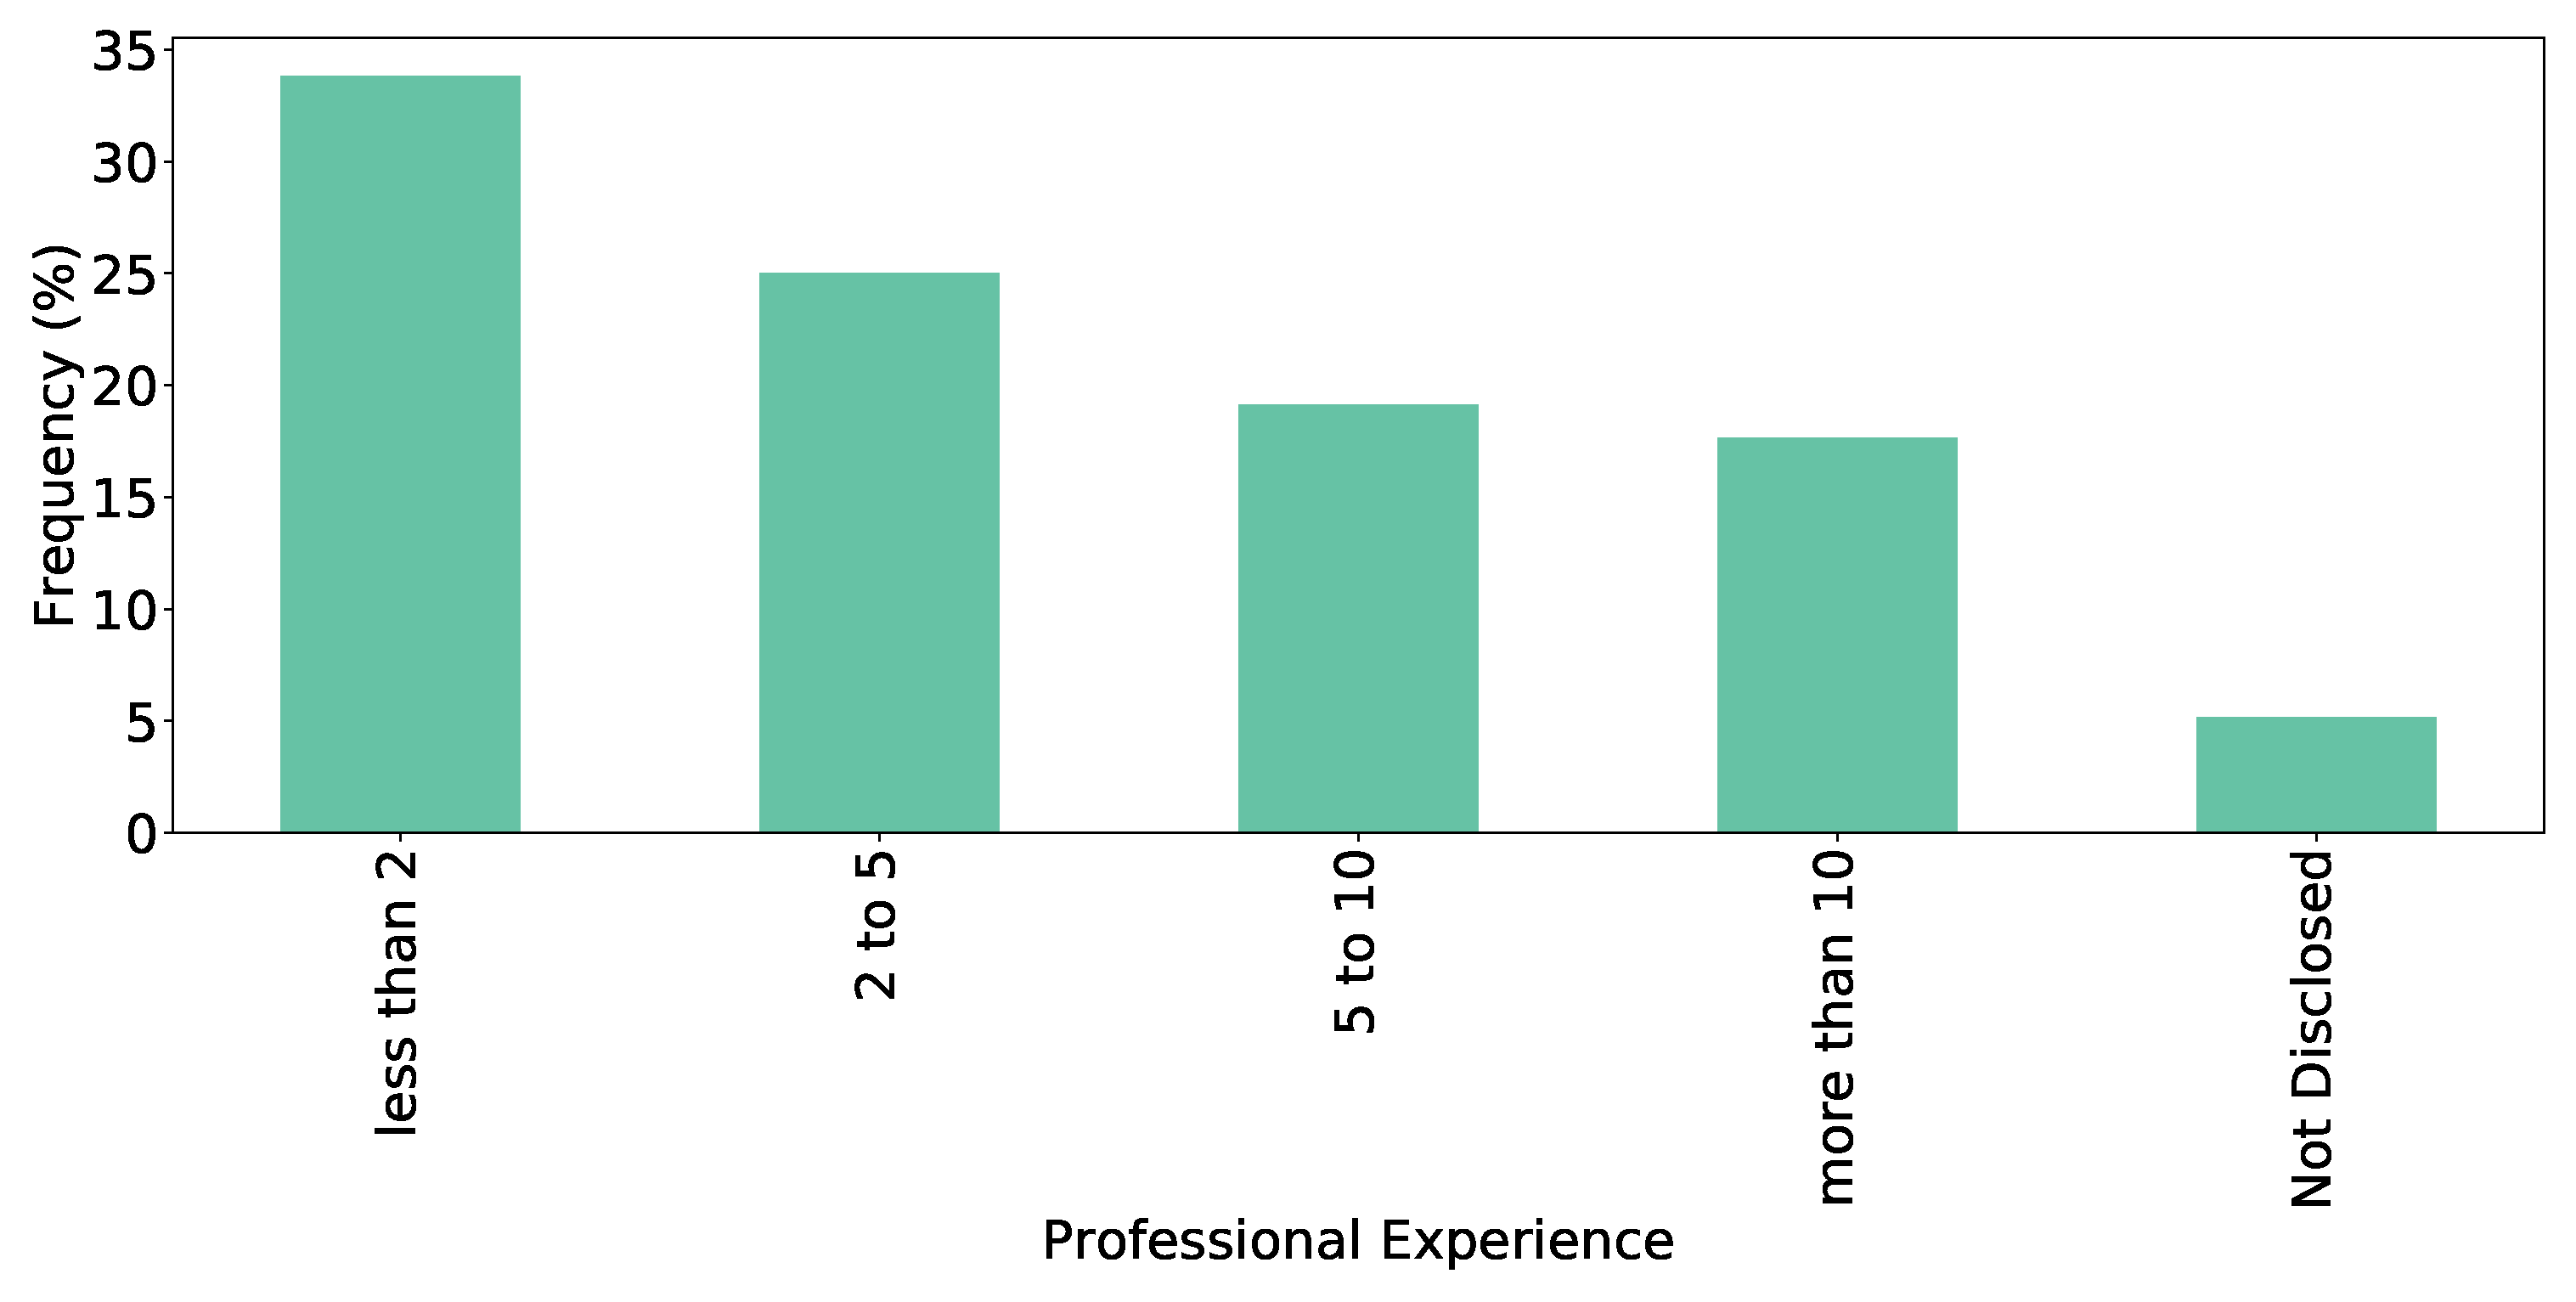
\includegraphics[width=0.8\textwidth]{Figures/Respondents_Experience}
  \caption{Work Experience}
  \label{fig:experience}
\end{figure}

\subsection{Respondent's Current Role}
From the \cref{fig:role} we see most of the respondents were software developers and approximately 15\% of our respondent's are working at manager level post which have appreciable impact on getting expectations from managers.
\begin{figure}[H]
\centering
  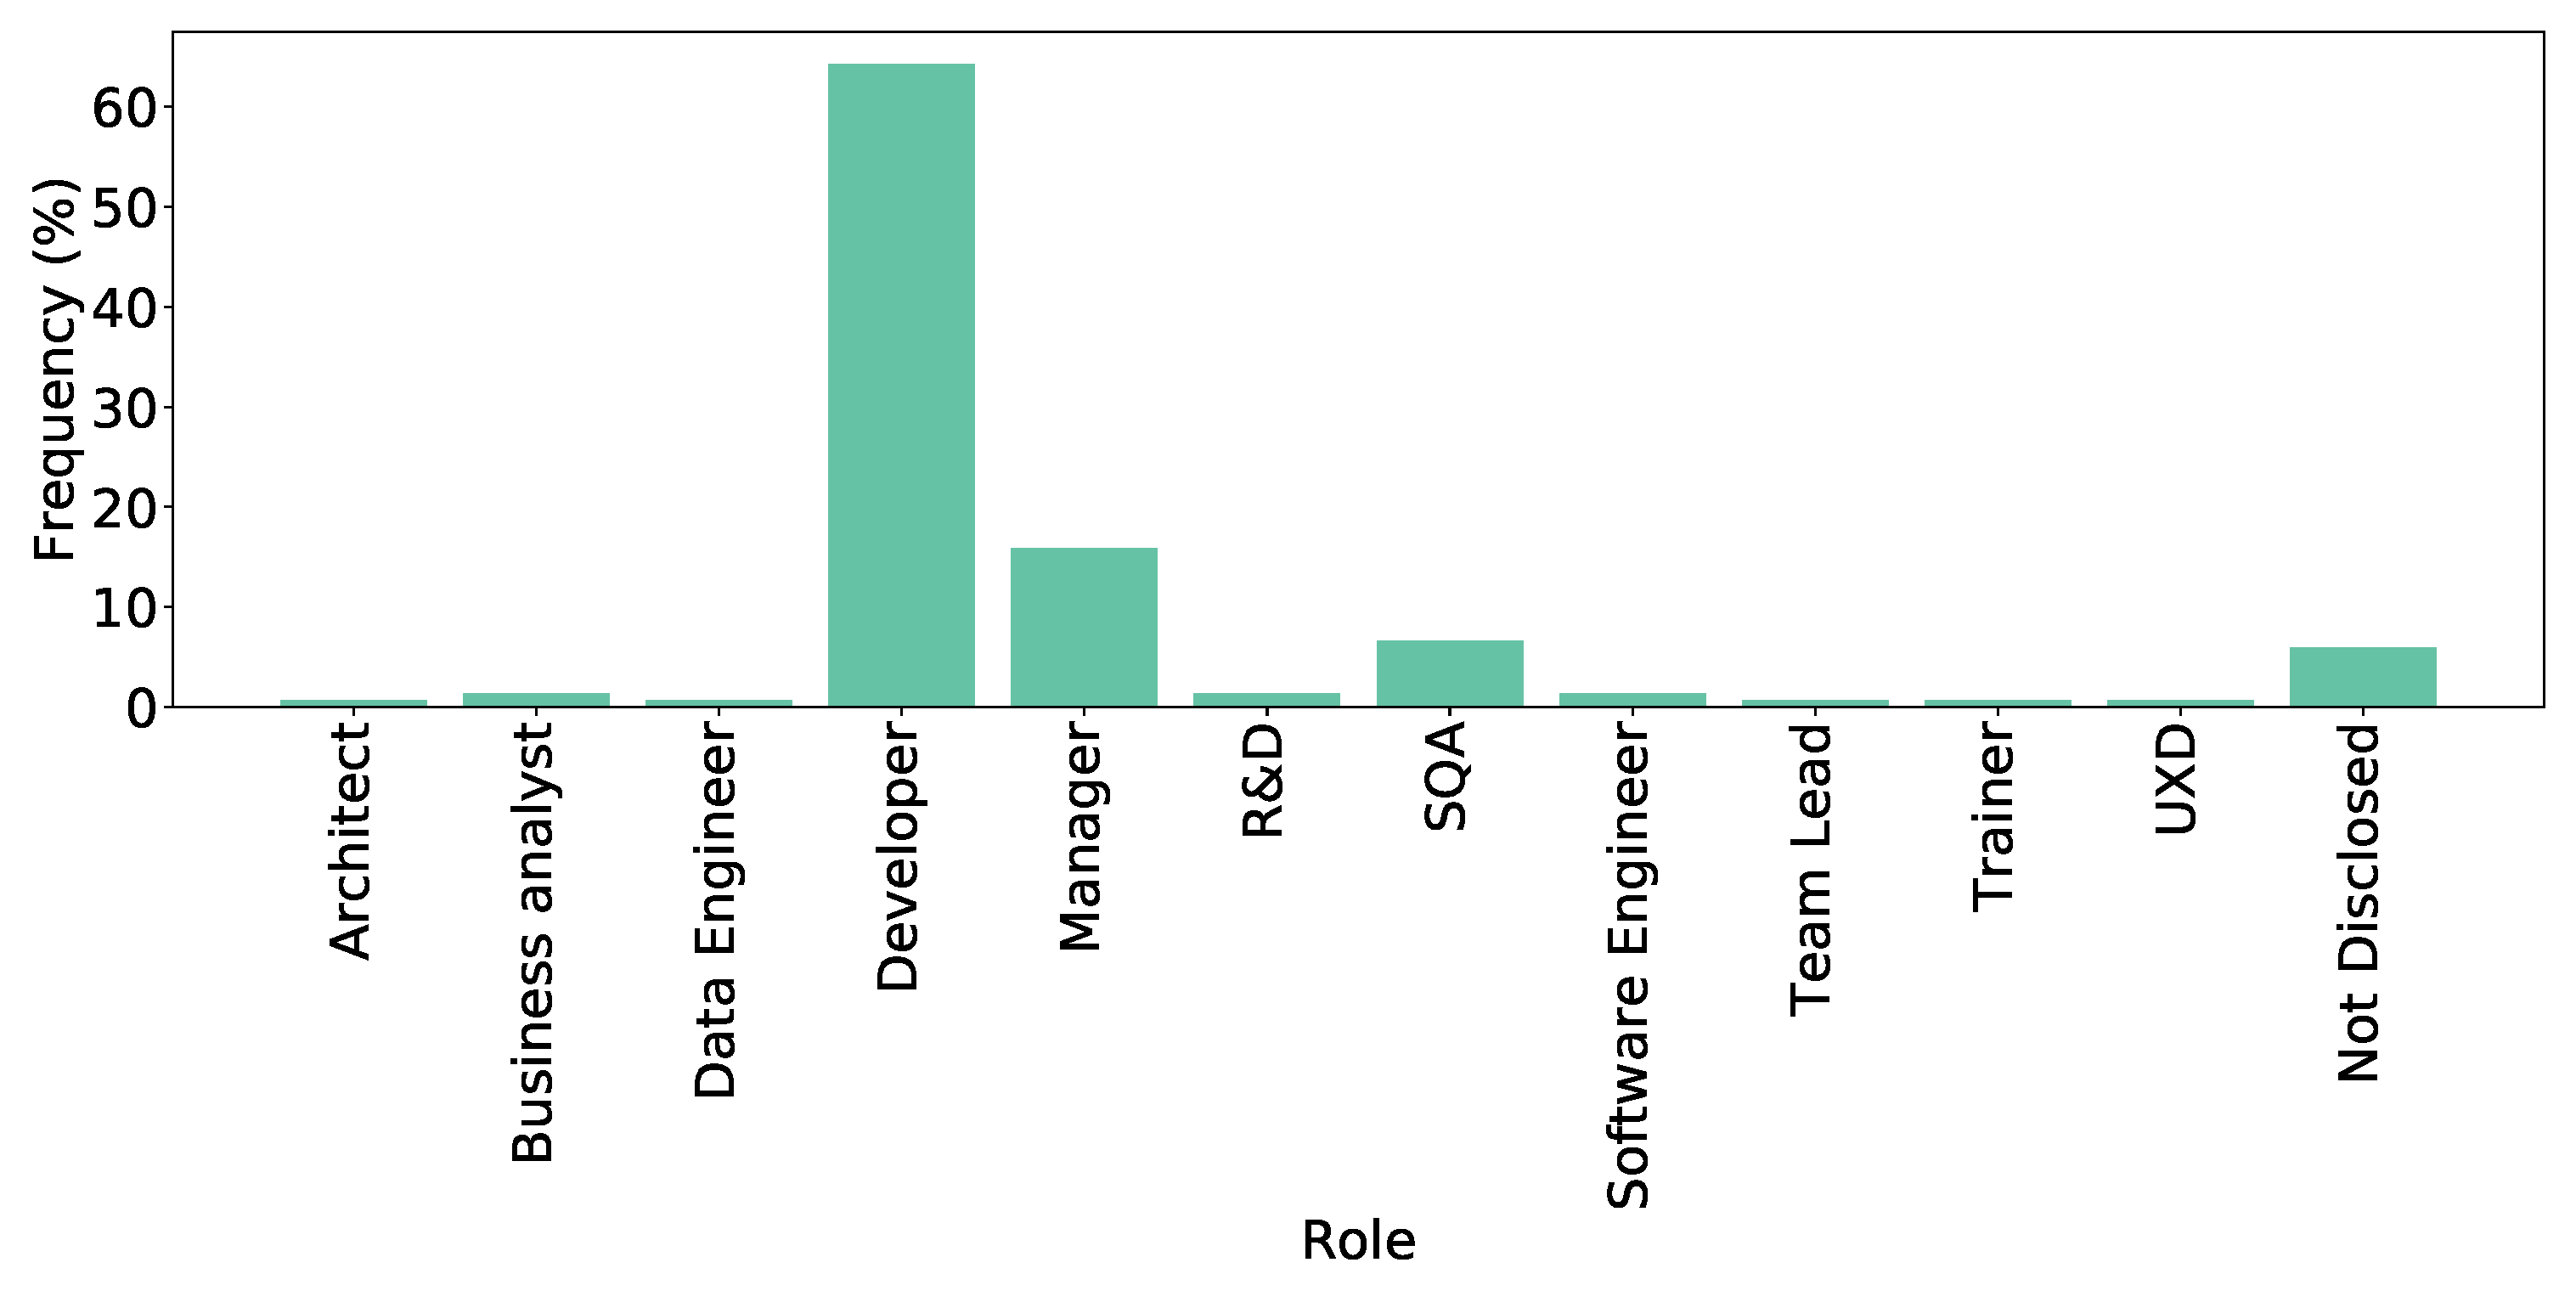
\includegraphics[width=0.8\textwidth]{Figures/Respondents_Role}
  \caption{Respondent's Current Role}
  \label{fig:role}
\end{figure}
%\section{Results}

\subsection{RQ1: What software methodology are used in your project?}
\label{RQ1}
Software development methodology in software engineering is a framework that is used to pursue the development of information systems in a very deliberate, structured and methodical way. To find out the overall answer of this question, we report the following results:
\begin{itemize}
\item Software development methodologies (Q 6).
\item Requirements gathering (Q 7).
\item Most time consuming software development activities (Q 8).
\end{itemize}

\subsubsection{Software development methodologies}
The most-widely used model is Agile with usage rate of 64\%. The next widely-used model is scrum with usage rates of 46\%. The other methodologies has lower usage rates, namely: pair programming (20\%), Waterfall (12\%) etc. From the study we see that the most acceptable model that was regularly and always used is the agile model in Bangladesh but the usage of the scrum (44\%) in New Zealand has greater usage followed by agile (30\%) \citep{Wang2018} and in Turkey, waterfall is mostly used based on the earlier 2015 survey \citep{Garousi2015}. Again, in both Bangladesh and New Zeland, extreme programming (XP) has a lower percentage of usage.
\begin{figure}[htbp]
\centering
  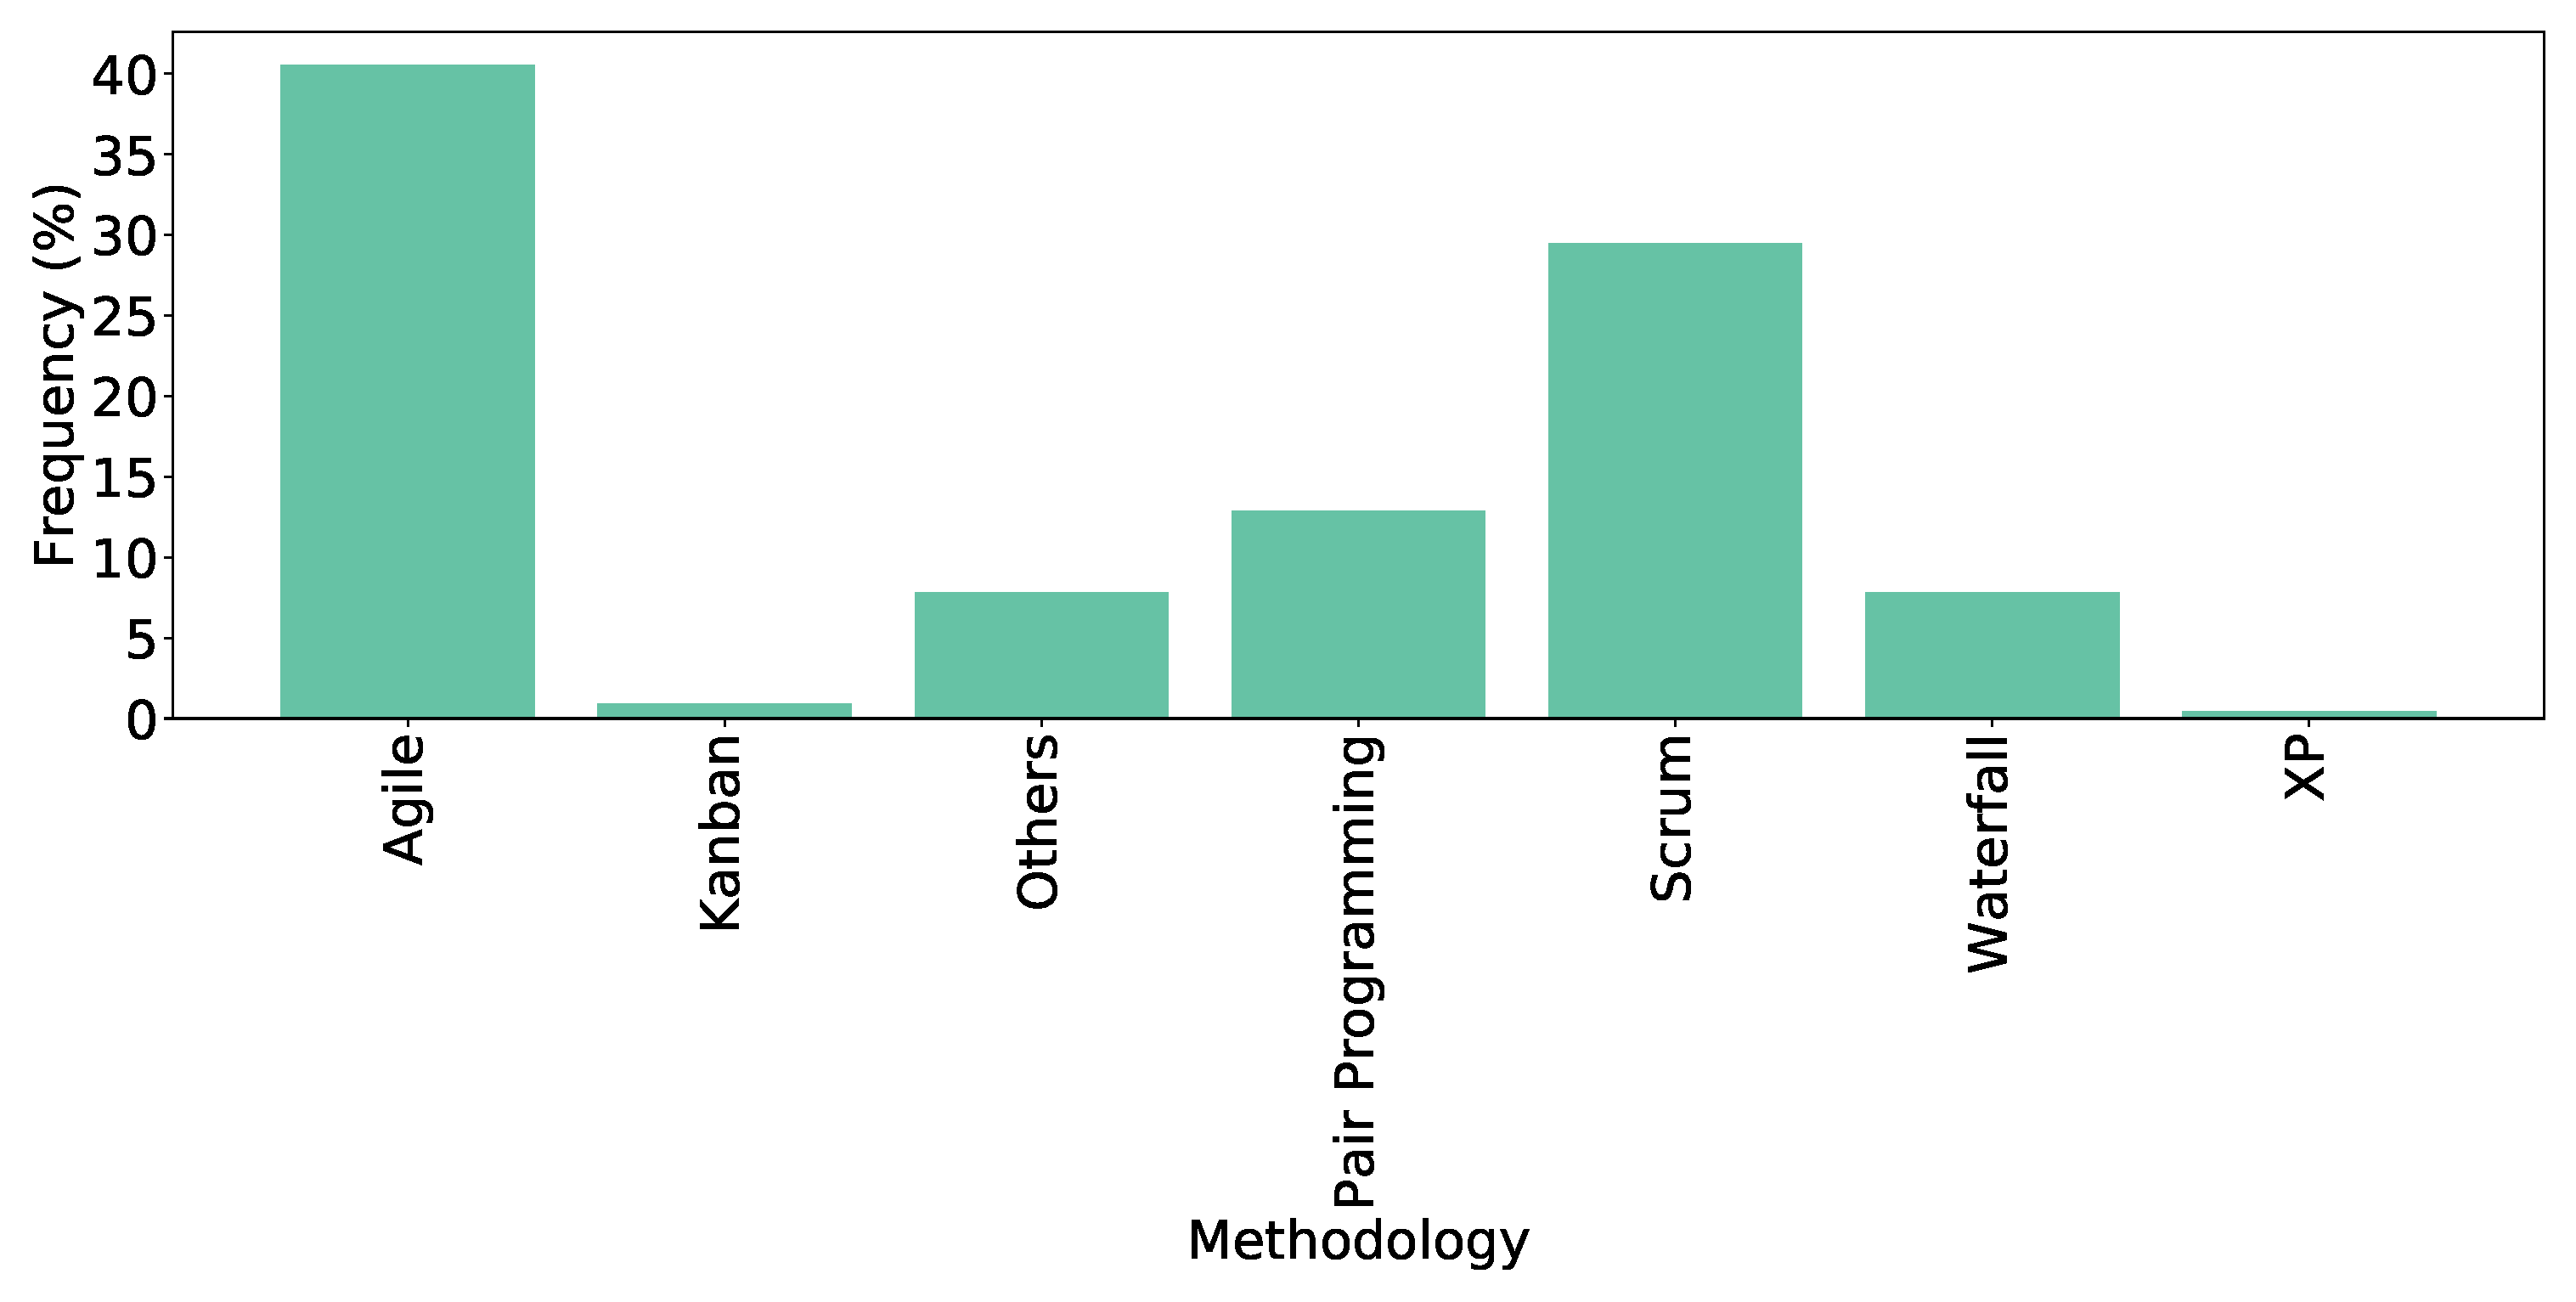
\includegraphics[width=0.8\textwidth]{Figures/Respondents_Methodology}
  \caption{Software development methodologies}
  \label{fig:methodologies}
\end{figure}

\subsubsection{Requirements Gathering}
The most critical activity that always arises during software development is the collecting requirement of the proposed system. According to \cref{fig:requirements}, using plain text (44\%) and story board (41\%) are the most widely used requirements gathering. This result is similar with the survey of Vonken et al. \citep{Vonken2012}. From their study we can find that the textual description of specifying requirements is a firm favourite in Netherlands. The other requirements gathering usage rates are: Use case (36\%), GUI prototype (35\%), grooming session (30\%) etc. This is an important finding that requires further analysis for causes and to analyze the potential effects of not documenting requirements.
\begin{figure}[htbp]
\centering
  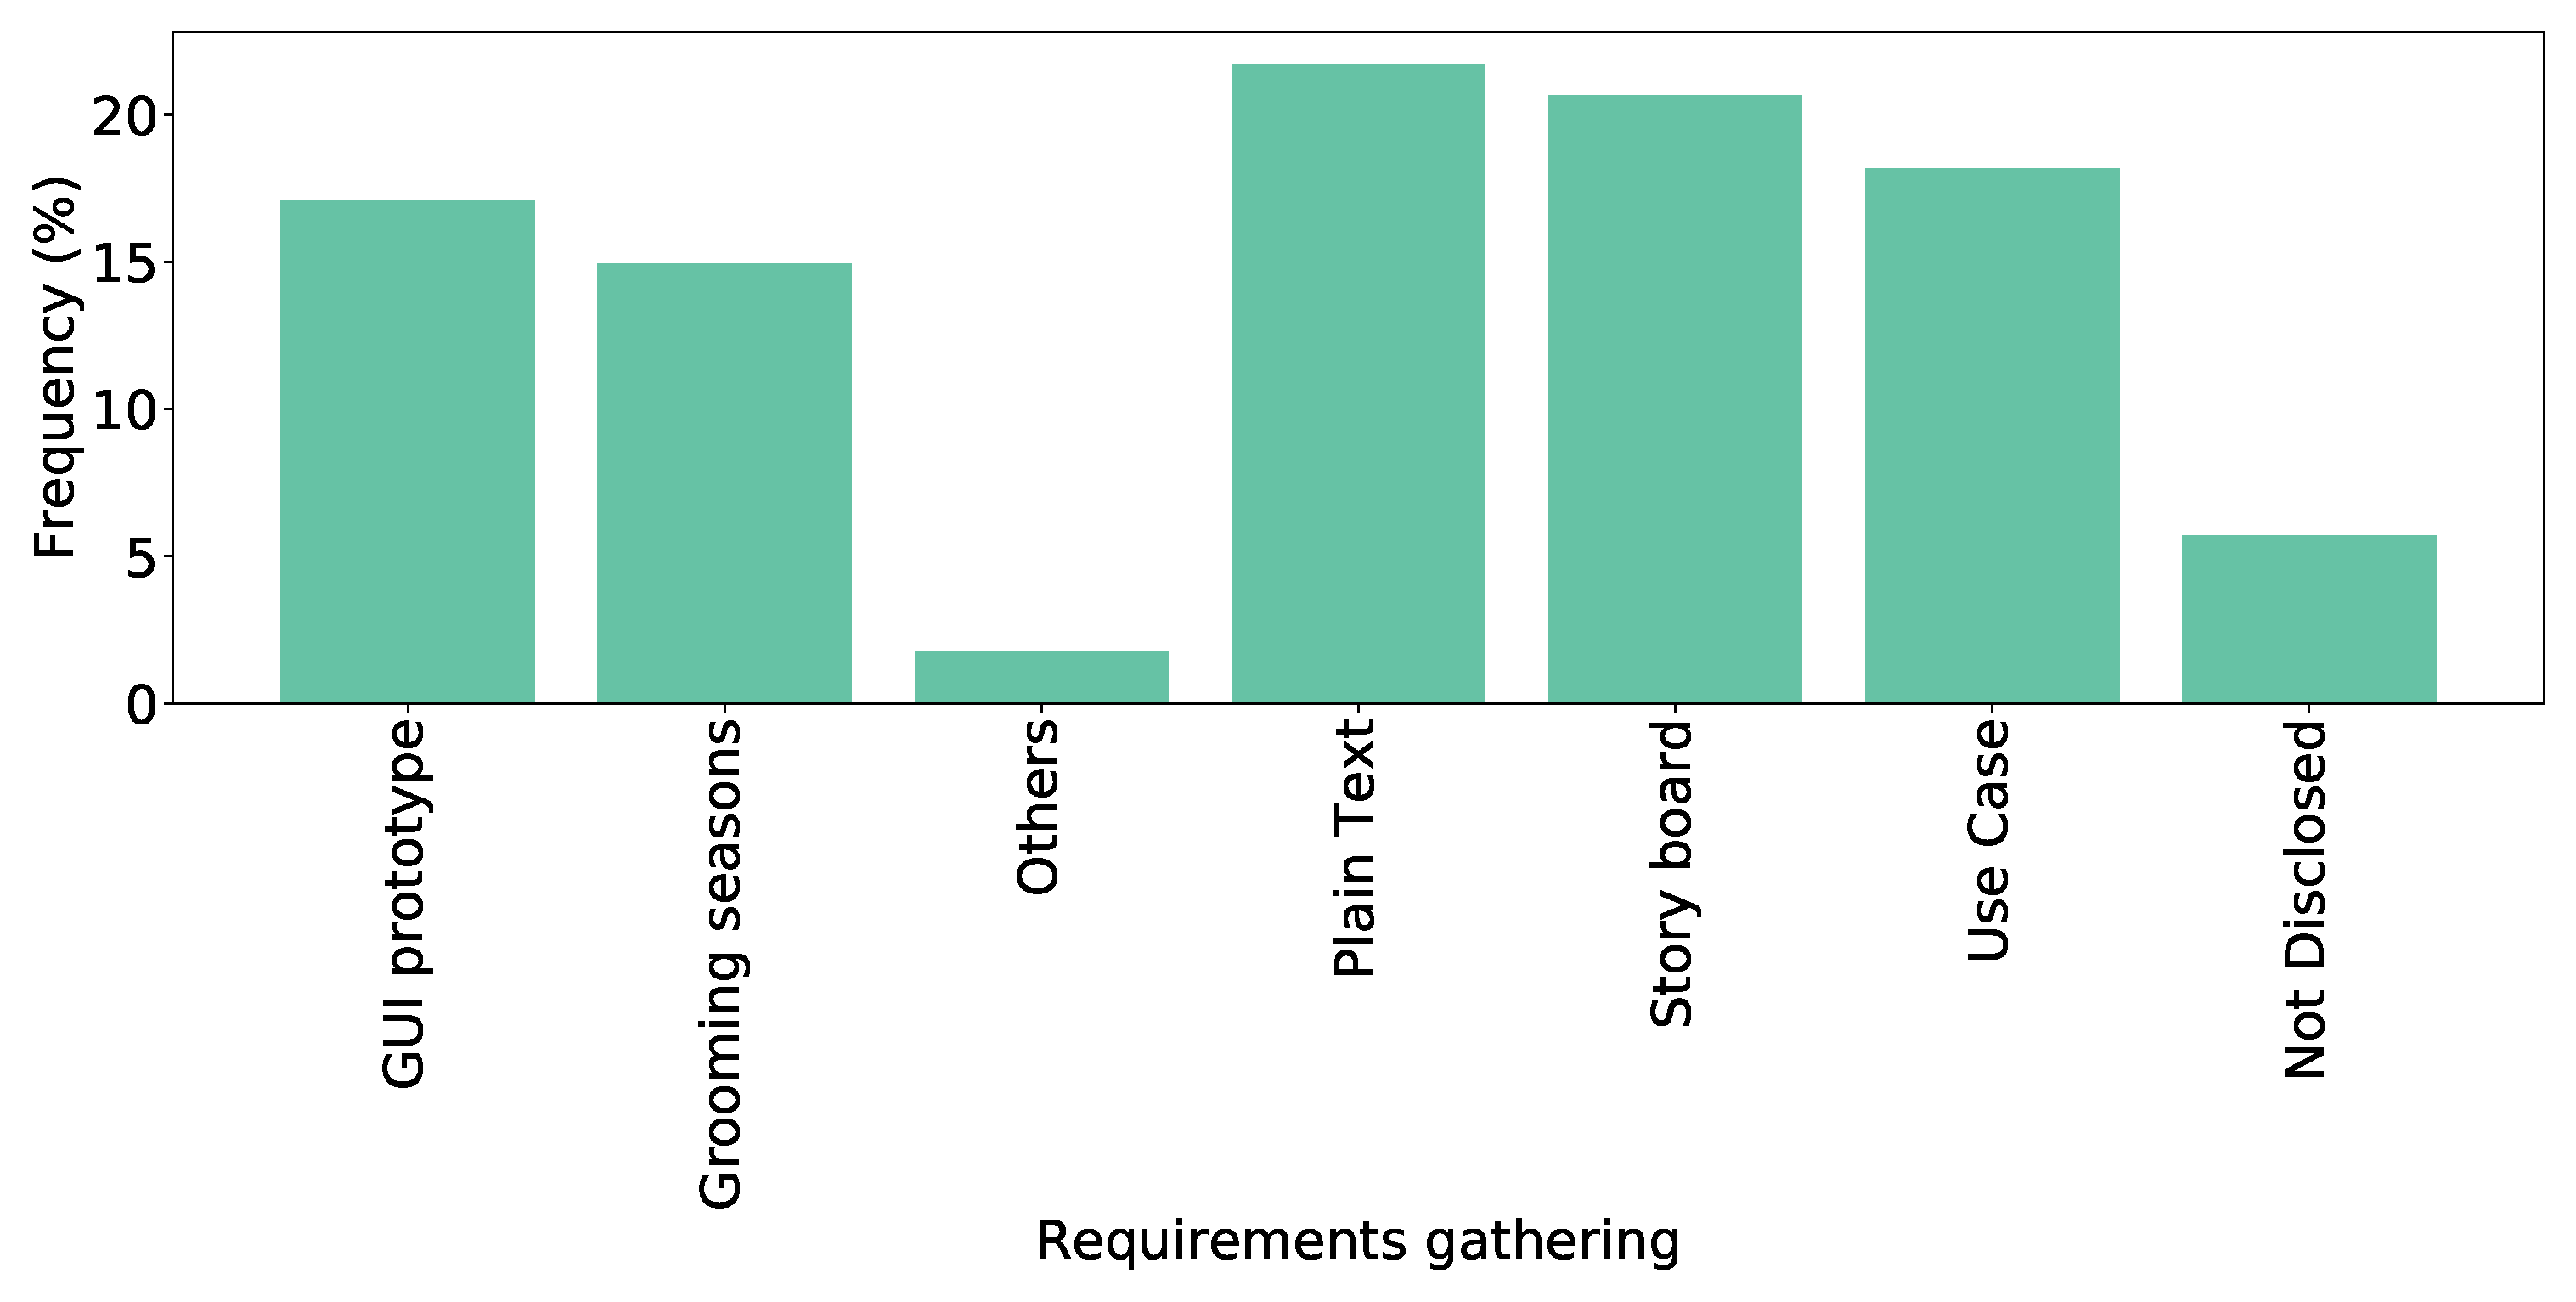
\includegraphics[width=0.8\textwidth]{Figures/Requirements_Gathering}
  \caption{Requirements gathering}
  \label{fig:requirements}
\end{figure}

\subsubsection{Development activities timeline}
In this section participants were asked about the most time consuming software developing activities they had spend. As we see in \cref{fig:activities}, most of the time spent in implementation stage according to 65\% our respondents and requirement analysis stage requires second most according to 45\% response. The other usages are: Program design (37\%), project planning (30\%), testing (19\%), maintenance (17\%) etc. According to study \citep{Wang2018}, most time was spent on implementation and coding and relatively less time was spent on maintenance in Bangladesh and New Zealand. But requirement analysis, the activity, requires the second most time to spend in Bangladesh where in New Zealand, it is testing (36\%) practices.

\begin{figure}[htbp]
\centering
  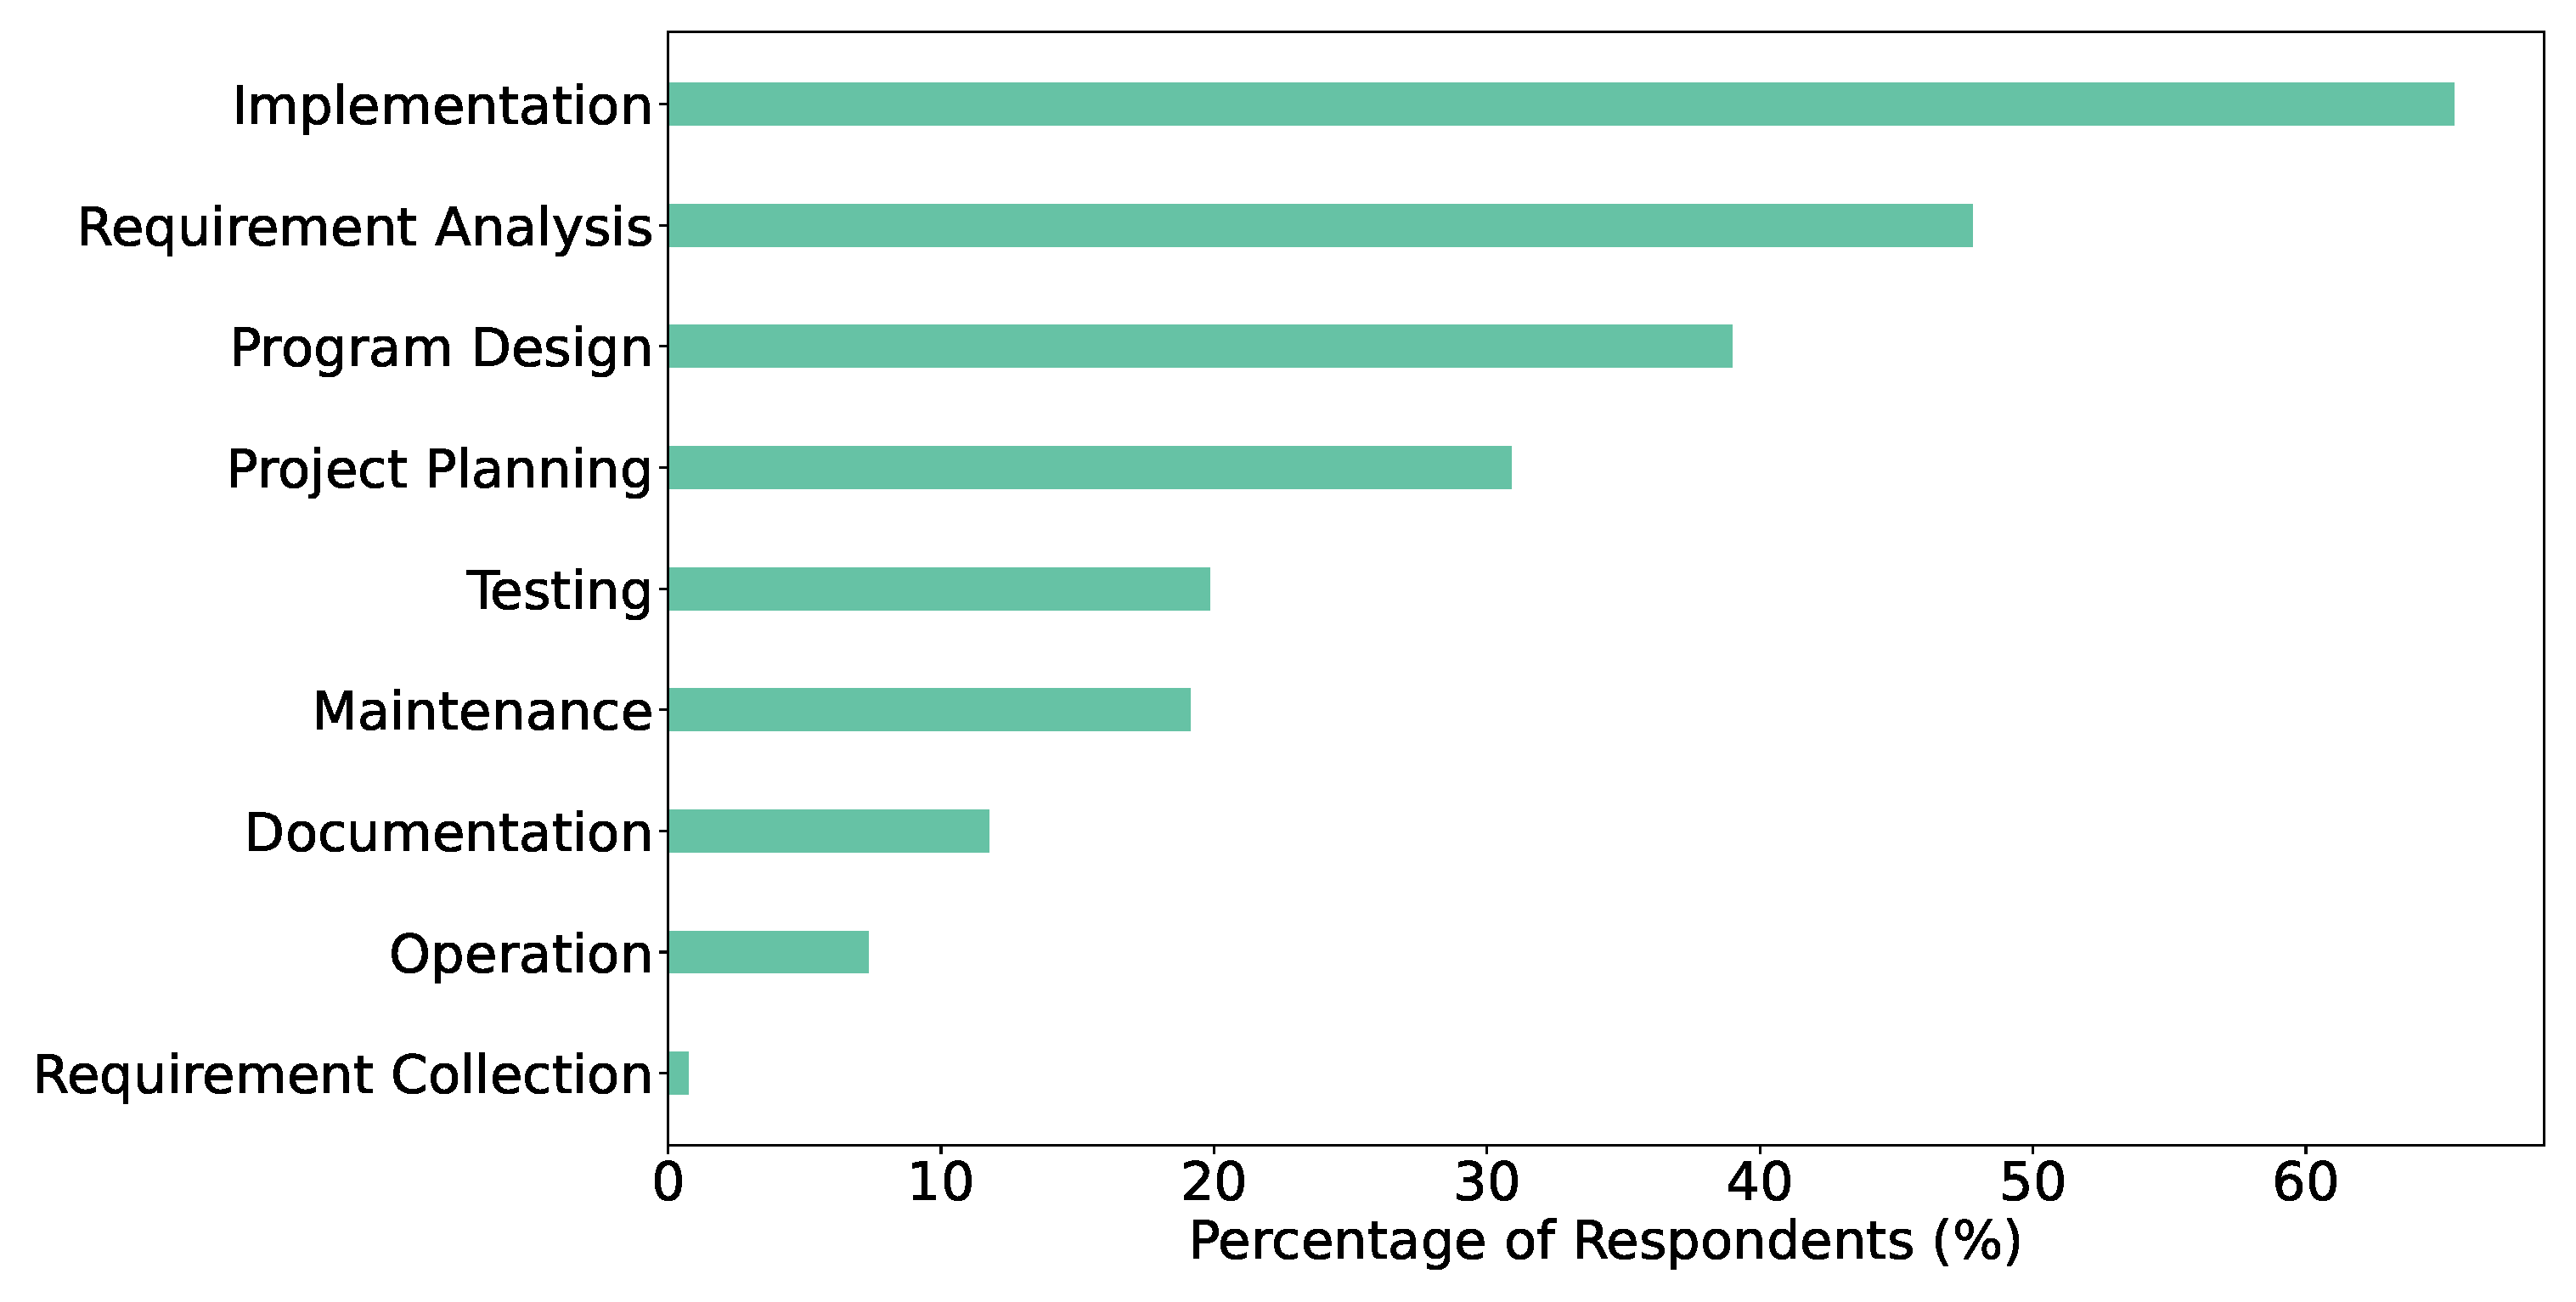
\includegraphics[width=0.8\textwidth]{Figures/Respondents_Activities}
  \caption{Software development activities}
  \label{fig:activities}
\end{figure}
\subsection{RQ2: Which implementation technologies and tools are adopted by software development professionals?}
\label{RQ2}
Our survey included five questions to find technologies and tools that are adopted by software development professionals. To answer this question fully, we report the following results:
\begin{itemize}
\item Technology Platform (Q 9).
\item Operating System (Q 10).
\item Programming Language (Q 11).
\item Framework (Q 12).
\item IDE (Q 13).
\end{itemize}

\subsubsection{Technology Platforms}
Participants were allowed to choose multiple options. As shown in \cref{fig:platforms}, most of the respondents (80\%) worked in web platform. The rests were mobile (45\%), Desktop (30\%), Embedded/IOT (8\%). Most respondents develop products and services for web platforms in both Bangladesh and New Zealand based on \#.
\begin{figure}[htbp]
\centering
  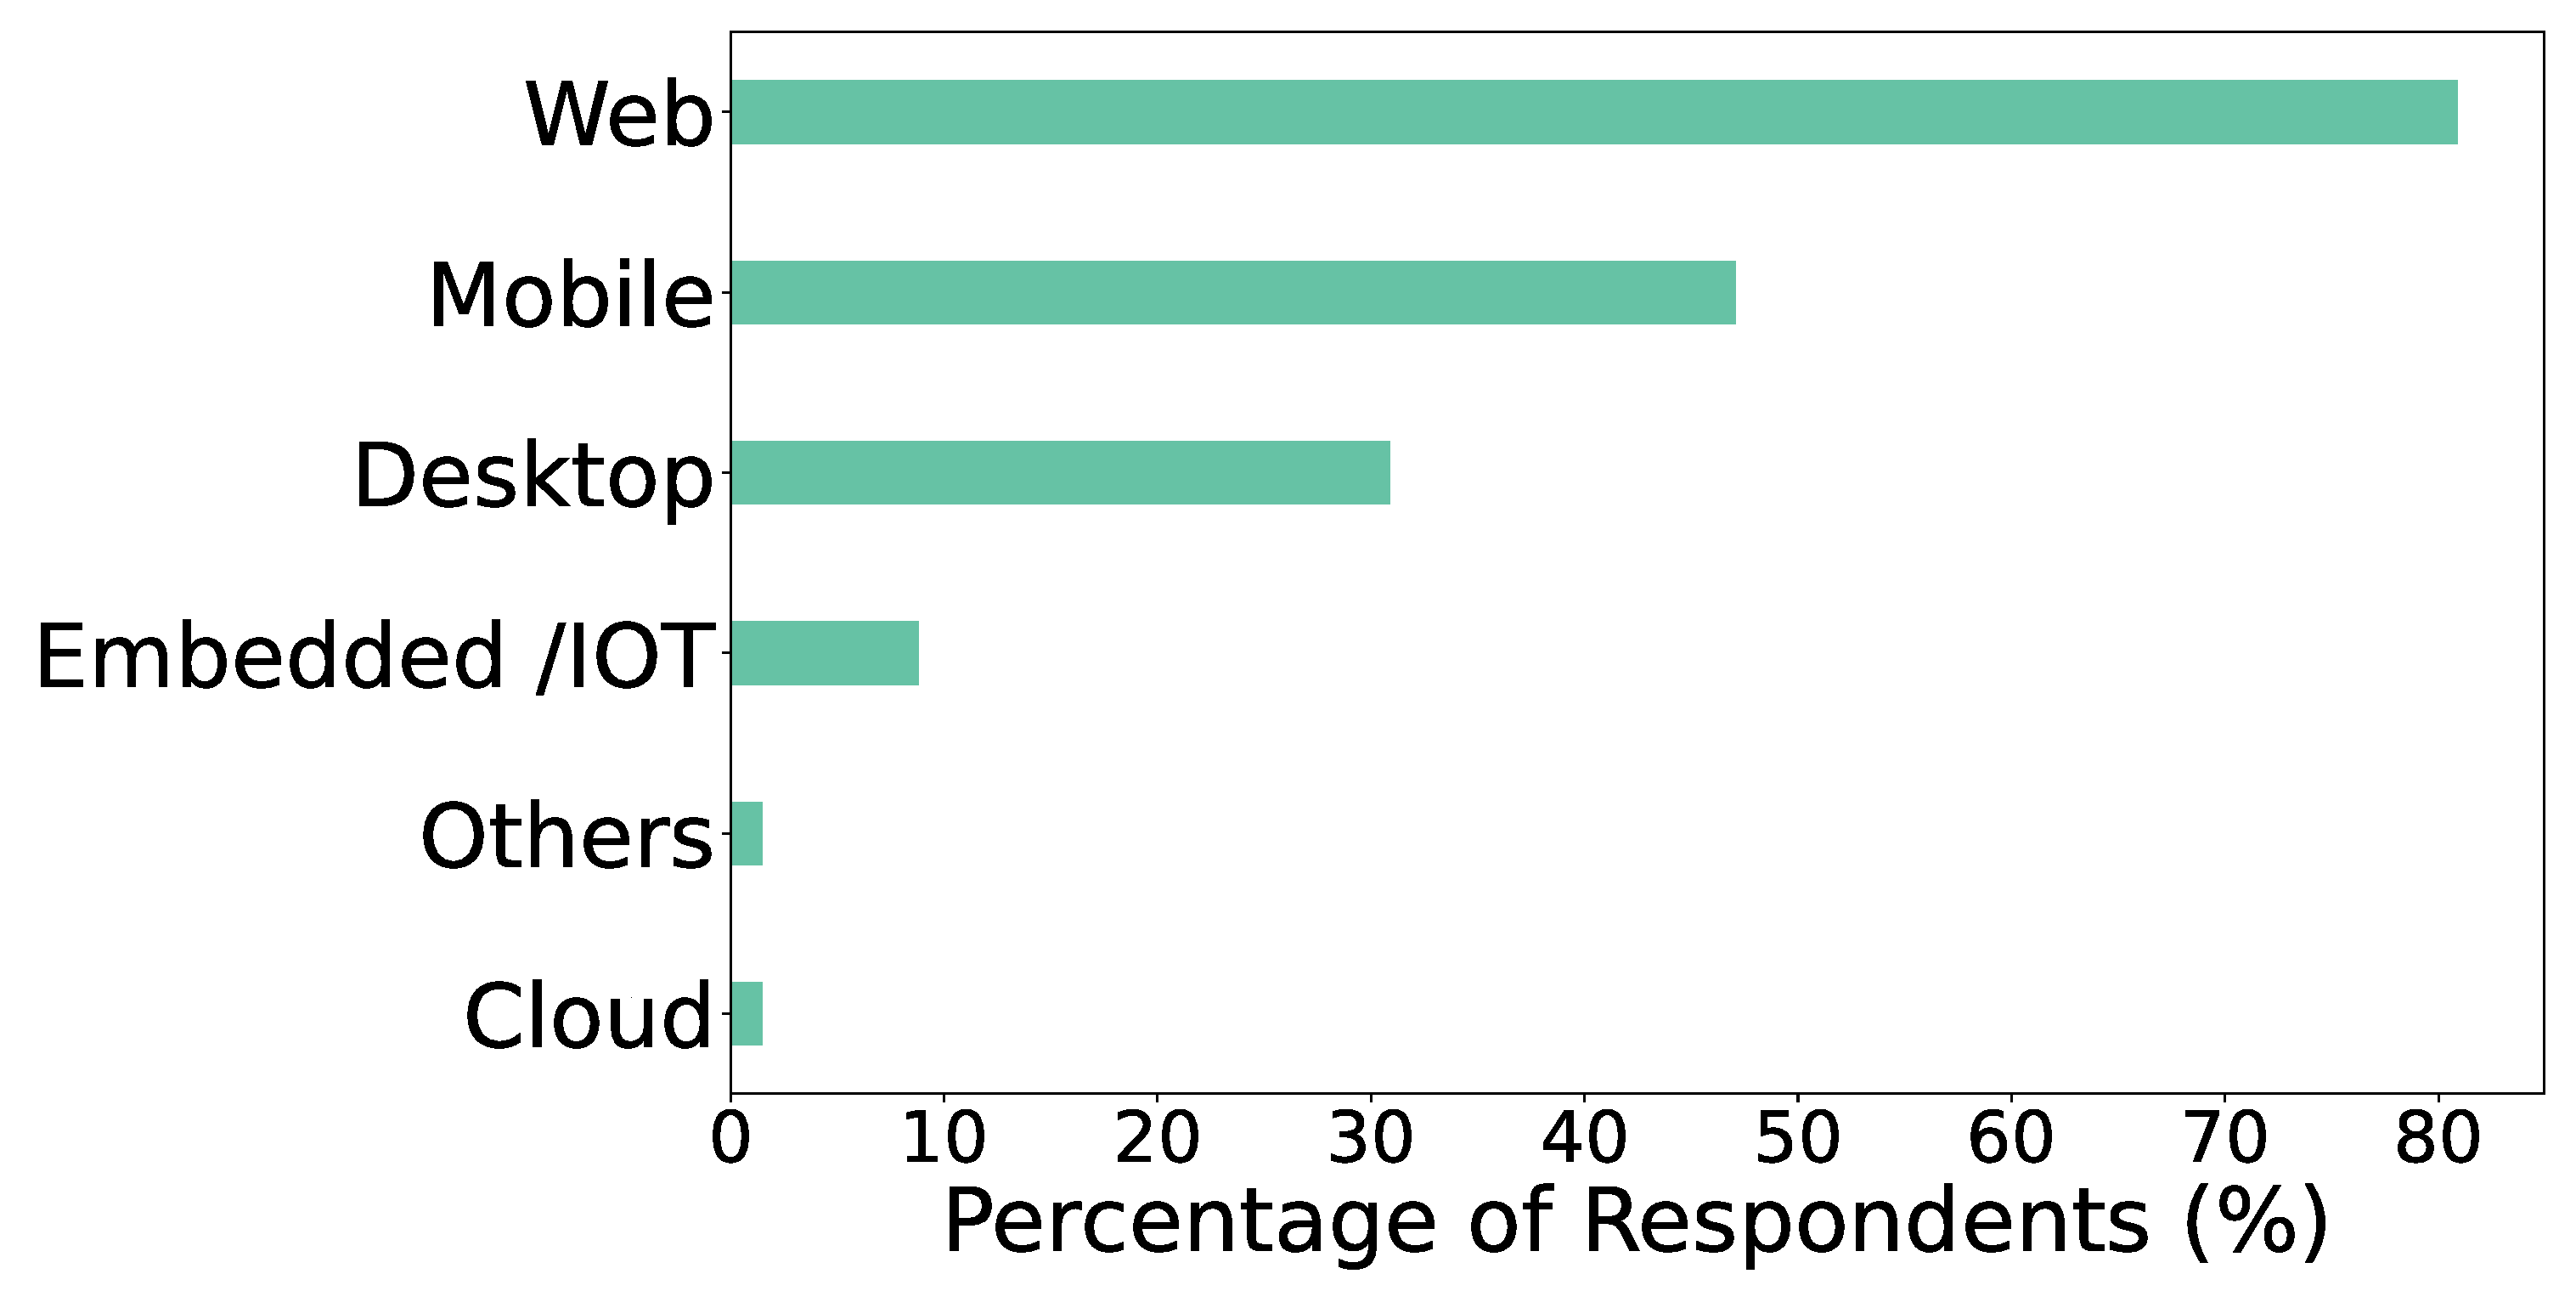
\includegraphics[width=0.8\textwidth]{Figures/Respondents_Technologies}
  \caption{Technology Platforms}
  \label{fig:platforms}
\end{figure}

\subsubsection{Operating Systems}
Most of our respondent's used linux based operating system (56\%). The second best used operating system is windows (45\%). Windows is mostly used among developers of New Zealand based on
the Survey \#, but linux is mostly used in the case for Bangladeshi developers.

\begin{figure}[htbp]
\centering
  \includegraphics[width=0.8\textwidth]{Figures/Respondents_os}
  \caption{Operating Systems}
  \label{fig:os}
\end{figure}

\subsubsection{Programming Languages}
According to \cref{fig:languages}, around 61\% of our respondent's used Java and Javascript each. Other languages like php (25\%), python (25\%), c\# (18\%) are also used which indicates that the software engineers are not inclined towards a single specific language. Also the choice of programming languages used for development can have important inferences for the testing practices of a software company. Based on \#, Java ranks quite low in New Zealand where it is the second most used in Bangladesh and the mostly used language in Turkey (\#). Again, python did not get a respective place in the rank of used languages in New Zealand but it is used significantly in Bangladesh.

\begin{figure}[htbp]
\centering
  \includegraphics[width=0.8\textwidth]{Figures/Respondents_languages}
  \caption{Languages used in software development}
  \label{fig:languages}
\end{figure}

\subsubsection{Frameworks used in development}
As shown in \cref{fig:frameworks}, variety of frameworks have been used during development. Spring boot (37\%) is the mostly used framework in the industry. ASP.NET, Django and Laravel are used in same proportion (14\%).
\begin{figure}[htbp]
\centering
  \includegraphics[width=0.8\textwidth]{Figures/Respondents_frameworks}
  \caption{Frameworks}
  \label{fig:frameworks}
\end{figure}

\subsubsection{IDE's used by the respondent's}
According to \cref{fig:IDEs}, IntelliJ, a Java integrated development environment for developing computer software for enterprise, mobile, and web development used by most of the respondents (43\%). The other IDEs used in SE industries are: visual studio (30\%), Eclipse (24\%), PyCharm (16\%), NetBeans (10\%), Android Studio (6\%).
\begin{figure}[htbp]
\centering
  \includegraphics[width=0.8\textwidth]{Figures/Respondents_IDEs}
  \caption{IDE's}
  \label{fig:IDEs}
\end{figure}

\subsection{RQ3: What type of testing and deployment practices are used?}
\label{RQ3}
Testing is an important process in improving the quality of the software product. The purpose of this process is to find errors, which might occur during specification, design and code generation. Here we report the following results next:
\begin{itemize}
\item Software Testing Practices (Q 14)
\item Level of Automated Testing (Q 15)
\item Tools Used in Testing and QA (Q 16)
\item Continuous Deployment tools (Q 17)
\item Version Control (Q 18)
\end{itemize}

\subsubsection{Software Testing Practices}
According to \cref{fig:testing}, several number of testing practices are used during software development. The results show most of the organizations carried out unit testing (53\%), functional testing (49\%), user acceptance testing (39\%), GUI testing (31\%) etc.
\begin{figure}[htbp]
\centering
  \includegraphics[width=0.8\textwidth]{Figures/Respondents_testing_practices}
  \caption{Testing Practices}
  \label{fig:testing}
\end{figure}

\subsubsection{Level of Automated Testing}
Question 15 asked about the level of automated testing. The responses were gathered using the Likert scale. This denotes that different respondents have very different practices in this context, i.e., some heavily practice automated testing, while others favor manual testing. Results are shown in \cref{fig:autoTest}.
\begin{figure}[htbp]
\centering
  \includegraphics[width=0.8\textwidth]{Figures/Respondents_autotest_level}
  \caption{Automated Testing Level}
  \label{fig:autoTest}
\end{figure}

\subsubsection{Tools Used in Testing and QA}
Q 16 asked about the tools used in testing and quality assurance. According to \cref{fig:testingTools}, we see that most of the respondents have been used XUnit( eg, JUnit, NUnit) (30\%), selenium (27\%), Jenkins (20\%), others (9\%). 
\begin{figure}[htbp]
\centering
  \includegraphics[width=0.8\textwidth]{Figures/Respondents_testing_tools}
  \caption{Testing \& QA Tools}
  \label{fig:testingTools}
\end{figure}

\subsubsection{Deployment Tools}
According to \cref{fig:deployTools}, wee see that most of the respondents use AWS code-deploy (12\%) and JenKins (12\%). The other deployment tools are Bamboo (5\%), teamcity (4\%), octopus (2\%). Respondents voted none (4\%) as they didn’t use any deployment tools.
\begin{figure}[htbp]
\centering
  \includegraphics[width=0.8\textwidth]{Figures/Respondents_deployment_tools}
  \caption{Deployment Tools}
  \label{fig:deployTools}
\end{figure}

\subsubsection{Version Control}
\hfill\\
Respondents were allowed to select more than one option. As shown in figure \ref{fig:versionControl}, Git (78\%) and BitBucket (29\%) are mostly-used version control in the software industry. Beside these SVN (5\%), others (4\%) are used.  The 2018 Stack overflow survey\citep{StackoverflowSurvey2018} reports that  the most popular version control system is Git (87.2\% developer uses Git) and the second most popular is SVN (16.1\% developer uses SVN). However, in our survey, we found slightly different result,the most popular version control system is Git and the second most popular is Bitbucket. This might be related  to the declining popularity of SVN over the years. From the Stack overflow survey over the range 2017-2019, it is clear that SVN is losing popularity to Git. Nowadays, SVN is mainly used for versioning legacy projects. As the SE industry of Bangladesh is quite new, we observe such discrepancy in the popularity of SVN.

\begin{figure}[htbp]
\centering
  \includegraphics[width=0.8\textwidth]{Figures/Respondents_version_control}
  \caption{Version Control}
  \label{fig:versionControl}
\end{figure}
\subsection{RQ4: How are the security and performance is ensured in a product of a company?}
\label{RQ4}
This particular question covers how a company secures its code from external attack and maintain its performance after deployment. It also slightly deals with the problem of scalability. Performance depends greatly on whether a product has scalability or not. So, we will cover the following points here:
\begin{itemize}
    \item Security
    \item Performance
    \item Scalability
\end{itemize}
\subsubsection{Security}
\label{Security}
\begin{figure}[htbp]
\includegraphics[scale=0.28]{Figures/Security.eps} 
\caption{Measures to maintain security of products}
\label{fig:Measures to ensure security}
\end{figure}
\hfill\\
Security refers to confidentiality, integrity and authenticity. To maintain security of software product SE industry of Bangladesh is mainly dependent on Standard process which includes cloud based security, third party software, OS hardening followed by uses of security tools, network level measures and framework security. As found by Harrison et al.\cite{Harrison2010} network level measures are the first choice in ensuring security of software product which matches with our findings. Srinivasan et al.\cite{Srinivasan2017} listed top 10 web framework in terms of security testing where Spring framework achieved 7\textsuperscript{th} position. From figure ~\ref{fig:frameworks} we have seen that most of our respondents use Spring framework for software development. This might be the reason that a lot number of respondents dependent on framework for ensuring security.
\begin{enumerate}

    \item \textbf{Application Side Measures}: Security is ensured at the software or application side. 2.19\% respondents implemented security measures at application level.
    \surveyquote{At application level, could not achieve others yet}{72}
    
    \item \textbf{Server Side Measures}: Security is ensured at the server side. 0.73\% respondents implemented security measures at server level.
    \surveyquote{We use github/bitbucket repository systems to code maintain and store. We use server side security on AWS and other third party server host.}{48}
    
    \item \textbf{Network level Measures}: Network level measures include IP-white-listing, port-blocking, VPN and  use of HTTPS  in software. 6.57\% respondents use at least one of the before mentioned strategy to ensure security.
    \surveyquote{network blocking and common security measures}{2}
    
    \item \textbf{Formal Verification}: Security threats can be mitigated by  a code level review . 1.46\% respondents ensured the practice of formal code review
    \surveyquote{There are some basic guidelines that we must follow and while code review this needs to be an absolute part that needs to be checked before the code gets merged}{112}
    
    \item \textbf{Measures for request forgery}: Measures against cross site forgery is implemented to ensure security. This includes CORS or cross origin resource sharing, CSRF or cross site request forgery or one click attack or XSRF. 2.19\% respondents implemented measures agianst  Cross-site request forgery to ensure security.
    \surveyquote{Security testings like: SQL injection, cross-site scripting, CSRF, API security, use of https,  detecting malicious / suspicious HTTP requests and auto-blocking}{42}

    \item \textbf{OAuth 2.0} : OAuth 2.0 is the industry-standard protocol for authorization. OAuth 2.0 focuses on client developer simplicity while providing specific authorization flows for web applications, desktop applications, mobile phones, and living room devices. Many (2.92\%) respondents use OAuth 2.0 protocol as the main way of maintaining security.
    \surveyquote{OAuth 2.0, JWT, Token Base Authentication, CORS Filter, XSRF}{127}
    
    \item \textbf{Token-based authentication} : A token-based authentication system allows users to enter their username and password in order to obtain a token which allows them to fetch a specific resource - without using their username and password. Once their token has been obtained, the user can offer the token which offers access to a specific resource for a time period - to the remote site. 5.11\% people expressed its eligibility.
    \surveyquote{Token based authentication for all of my rest service}{80}
    
    \item \textbf{Multi-prong Standard Process} : Following multiprong standard processes is the best way to enforce security. About 10.22\% of the total respondents expressed this opinion.
    \surveyquote{Multi Prong Standard Processes and Products}{110}
    
    
    \item \textbf{Encryption at Various Levels} : Not only at password,but also in every level of software, encryption is first and foremost to ensure its security.
    \surveyquote{use encryption at different level of software (server, network, transmission layer, database and software layer.)}{35}
    
    \item \textbf{Use of tools} : Respondents use various open-source/ paid tools for scanning  and testing. These tools help to find security threats in an existing system. The tools includes OWASP based tools and  penetration testing tools
    \surveyquote{use encryption at different level of software (server, network, transmission layer, database and software layer.)}{35}
    
    
    \item \textbf{Dependent on Framework} : Common framework provides basic to intermediate level security measures in the application. 6.57\% respondents depends on framework for security. The framework includes spring and  HDIV.
    \surveyquote{https, popular framework which already prevents some type of attacks. rest of the things on case-by-case basis)}{79}
    
    
    \item \textbf{Non-disclosure agreement} : 2.19\% refused to provide any details due to non-disclosure agreement.
    \surveyquote{As we are regulated by Bangladesh Bank as a payment processing platform, we need to maintain certain security compliance which cannot be disclosed here. The security compliance is similar to the PCI DSS compliance which I can say}{10}
    
    \item \textbf{Continuous Upgrading}: As security threats are evolving thus current systems need continuous upgradation in a frequent interval. 1.46\% respondents said they arrange frequent hackathon, workshop, security audits to address the continuously evolving security threat.
    \surveyquote{We run security audit of our office environment. We also conduct security session per 6 months to introduce latest trend in threats and what we can do to avoid it}{57}
    

   
\end{enumerate}

\subsubsection{Performance}
\label{Performance}
\begin{figure}[htbp]
\includegraphics[scale=0.28]{Figures/Performance.eps} 
\caption{Measures to ensure performance of products}
\label{fig:Measures to ensure performance}
\end{figure}
\hfill\\
Software performance indicates how efficient the software is in terms if resource and time. Testing tools such as load testing are common measure\cite{Liu2009} to ensure performance of a software on this regard Bangladesh SE industry follows the same measures. According to our respondents the top three performance ensuring method in Bangladesh SE industry is use of tools, test and better codes/practices or design-implementation level measures. 
\begin{enumerate}

    \item \textbf{Caching Mechanism}: Caching mechanism improves performance by reducing response time. 
    \surveyquote{... Good Caching}{29}
    
    
    \item \textbf{Emphasize on design}: Software performance is dependent on architecture of system. 5.84\% respondents emphasize on design to ensure performance.
    \surveyquote{By careful designing}{24}
    
    
    \item \textbf{Testing}: Performance is ensured by various rigorous testing phase. The phase includes load testing, stress testing, integration testing.
    \surveyquote{By rigorous testing and checking performance testing}{17}
    
    
    \item \textbf{Emphasize on Infrastructure}: 5.11\% respondents use upgraded infrastructure to ensure performance. These infrastructure includes cloud hosting, high end server, new technologies.
    \surveyquote{Amazon Hosting and Quality Software}{85}
    
    
    \item \textbf{Implementing best practices}: Industry standard best practices can improve system performance. 7.3\%respondents ensure performance by implementing best practices. The best practices include compression technology, enforcing design patterns and refactoring.
    \surveyquote{Implementation time carefulness and maintaining a well developed coding standard}{40}
    
    
    \item \textbf{Load Balancing}: Load balancing can improve the system performance by ensuring equal load to all servers. 27.1\% respondents think of using load balancing as a measure to maintain performance.
    \surveyquote{Optimizing number of HTTP requests, Asynchronous programming, Caching, CDN, Load Balancing, nginx, varnish, compression of data, Continuous monitoring, Load testing, stress testing}{42}
    
    \item \textbf{Performance Monitoring Tools}: There are various performance monitoring automated tools from which we can measure the overall as well as component-wise performance of a product. 10.95\% respondents use these tools to measure performance.
    \surveyquote{take help of different performance monitoring tools and dashboard, analyzed data , measure time and memory efficiency of process}{35}
    
    \item \textbf{User Feedback}: It is a great source of performance measure. Taking a time to time feedback from the clients help a company to realise how their products are performing actually. Many (4.38\%) respondents have highly recommended it.
    \surveyquote{Continuous feedback from clients and QA team}{65}
    
    \item \textbf{Continual Evaluation}: If there are some problems about performance, it can easily be identified in continuous monitoring and evaluation of the products. 6.57\% of the total respondents have thought of this as a better solution.
    \surveyquote{regular rechecking/running of automation scripts as a automation tester}{14}
    
    \item \textbf{Code Review}: About 2.92\% people have said that a proper and attentive code review can reduce the faults in the codes and therefore enhance the performance of a software.
    \surveyquote{The code quality is assessed by the different team members during code review, followed by designing new ways to solve issues in the product that are time-intensive.}{15}
\end{enumerate}

\subsubsection{Scalability}
\label{Scalability}
\begin{figure}[htbp]
\includegraphics[scale=0.28]{Figures/Scalability.eps} 
\caption{Measures to ensure scalability of products}
\label{fig:Measures to ensure scalability}
\end{figure}
\hfill\\
 Software scalability defines the ability to scale up a solution. Issues with little importance can impede scaling up. Thus proper measures should be taken from design stage to ensure the scalability of system. Recent days the cloud services offer tools to accomodate custom reactive scaling strategies. Thus, it has become easier to ensure scalability using cloud services \cite{Falatah2014}. Our results  also follows the world trend, usage of cloud services has placed 2\textsuperscript{nd} in terms popularity of scalability measures in SE industry of Bangladesh.
\begin{enumerate}
    
    \item \textbf{Following Certain Design Patterns}: There are some design patterns which inherently help us in time of scaling. 5.84\% people think that Following these design patterns will be of great use.
    \surveyquote{Following certain design patterns}{8}
    
    \item \textbf{Based on Framework}: Modern frameworks ensures scalability by default. 0.73\% respondents solely depends on framework for scalability.
    \surveyquote{following flexible framework which allows better scalability}{14}
    
    
    \item \textbf{Container Technology}: Container technologies includes docker, Kubernetes which ensures OS level virtualization. By standardizing the system, container technologies eases the scaling of an infrastructure.
    \surveyquote{We used Docker technology}{85}
    
    \item \textbf{Database Optimization}: Database optimization includes sharding, clustering, indexing and scaling. 10.3\% respondents optimize database to scale their system.
    \surveyquote{Besides scaling horizontally, database scaling is performed by partitioning tables, along with multi-threaded implementations}{85}
    
    \item \textbf{Efficient Design and Implementation}: 12.41\% respondents emphasizes on  the design and implementation of a scalable architecture.
    \surveyquote{During implementation we always keep in mind about the scaling factor}{40}
    
    \item \textbf{Emphasizing on architecture}: 7.3\% respondents emphasized on architecture. It is mostly micro-service architecture which they use to ensure scalability.
    \surveyquote{We follow the micro-service architecture. In a nutshell, we scale up the module vertically which is necessary. We use docker along with Jenkins for automatic deployments and scaling.}{10}
    
    \item \textbf{Load Testing}: Load testing can be used to check the scalability of a system. 4.38\% respondents use load test to check wheather their system is scalable or not.
    \surveyquote{through load testing and load simulation.}{35}
    
    \item \textbf{Using Cloud Services}: 10.95\% user depends on Clod services like AWS and Azure  for the scalability of system. Modern features like elastic load balancing and  auto- scaling makes it easy to ensure scalability.
    \surveyquote{Using AWS Elastic Load Balancer}{28}
    
    
    
\end{enumerate}

\subsection{RQ5:What are the personal expectations and desire reigning in the industry?}
\label{RQ5}
This is the most interesting question. In fact, this question truly answers about the existing condition of our software industry. There are many problems and every one of them has solution. All about these have come into this question beautifully. Every employee has something to tell to their managers. Likewise, every manager has some demands from his subordinates. Not only these, they all have some expectations from government and also universities. All of these expectations are included in the answer of this research question.

\begin{itemize}
    \item Expectation from Managers
    \item Expectation from Employees
    \item Expectation from Potential Candidates
    \item Expectation from Universities
    \item Expectation from Government
    \item Training provide by Companies
\end{itemize}


\subsubsection{Expectation from Managers}
\label{Expectation from Managers}
\begin{figure}[htbp]
\includegraphics[scale=0.28]{Figures/Managers_Expectation.eps} 
\caption{Respondents expectation from managers}
\label{fig:managers expectation}
\end{figure}

\begin{enumerate}
    \item \textbf{Proper behavioural manner}: 6.57\% respondents expect well behaviour from management. It is clear from survey responses employees hates micro-management the most.
     \surveyquote{Well Behaved and Proper Project Timeline}{28}
    
    
    \item \textbf{Being Reasonable}:  The managers should be reasonable in decision making. In order to get acquainted with the needs and necessities of the employees, managers should have a wide open view towards their desire. About 8.03\% of the respondents have expressed in this way.
    \surveyquote{Give reasonable time for a task and do proper comment on that task}{38}
    
    
    \item \textbf{Flexibility of Technology}: It is very important for the managers to be up-to-date with the latest technology. Managers without a strong background of technical knowledge are really difficult to work with. 4.38\% of total respondents have demanded for a manager with sufficient technical knowledge. 
    \surveyquote{Allow to use latest technologies and good practice to ensure company and their employee are updated with the current world. And also honor according to knowledge and quality works. In the company should have knowledge sharing, training sessions}{48}
    
    
    
    \item \textbf{Responsibility}: Managers should take the responsibility for the works being done. A responsible manager can inspire the employees under him to a great extent. About 5.84\% of the total respondents aspire for a responsible manager to work with.
    \surveyquote{Take responsibility}{82}
    
    
    \item\textbf{Facility Improvement}: 11.68\% respondents mentioned that they look for facility improvements from managers. These facilities include increased remuneration, good working environments, team building events, positive recognition, yearly evaluation etc.
    \surveyquote{Ensuring an environment where positive criticisms regarding code and people can be done.}{57}
    
    
    \item\textbf{Inter Personal Skill}: 8.03\% respondents expects inter personal skills among managers. The skills include proactive, leadership attitude, good communication skill and empathy.
    \surveyquote{Ownership, Proactiveness, Leadership attitude, Good inter-personal and communication skills}{42}
    
    
    \item\textbf{Managerial Skill}: The managers should have solid technical knowledge. He/she must be farsighted. One of the most important part of this post is management of requirements. He should have clear  understanding of required manpower and resources. Respondents marked that timeline management is another managerial skill they expect from managers.
    \surveyquote{1. Strong grasp on the requirements before assigning me to a project 2. Maintain informed and feasible deadlines}{8}
    
    
    \item \textbf{Mentoring}: Respondents also look  a mentor character in manager. They expect direction, advice and opportunity from managers for their career growth.
    \surveyquote{To supervise and to advise to follow specific career plan}{9}
    
    
    \item\textbf{Sound Technical Knowledge}: 11.68\% respondents emphasizes on technical knowledge among managers.
    \surveyquote{Should be technically active}{14}

\end{enumerate}


\subsubsection{Expectation from Employees}
\label{Expectation from Employees}
\begin{figure}[htbp]
\includegraphics[scale=0.28]{Figures/EmployeeExpectation.eps} 
\caption{Respondents expectation from employees}
\label{fig:employees expectation}
\end{figure}

\begin{enumerate}

    \item \textbf{Technical Knowledge}: 3.65\% respondents look for solid technical knowledge and clean codes from employees.
    \surveyquote{Code in a way that is a delight to read}{49}
    
    
    
    \item \textbf{Teamwork}:It is very obvious to be expected. In a software industry, not a single product is created single-handedly. A bunch of people from various sectors work on the product, and to make a good product, team work between these members is very important. 5.84\% of the managers responded desired this behaviour from the employees.
    \surveyquote{Employees should be cooperative and share knowledge with each other and work together like family member}{51}
    
    
    \item \textbf{Self Initiative}: An employee should learn in his own interest. In industry, everyone is occupied with himself. There is no space to be spoon-fed. A self-initiative worker will find his way even if there are many obstacles.8.03\% people have appraised self-initiative attitude.
    \surveyquote{Clean code which creates less error. Coming up with optimization proposals on features developed earlier. Documentation in a timely manner}{10}


    \item \textbf{Leadership}: 4.38\% respondents look for leadership attitude like ownership of work, proactive and adaptiveness among employees.
    \surveyquote{Sincere, Feel owner ship of project/product and good teamplayer}{107}
    
    \item \textbf{Honesty and Integrity}: Not only coding and academic knowledge, but also behavioural manner plays a great role in deciding about a employee’s career. 3.65\% people want a well behaved and mannered employee to work with.
    \surveyquote{honesty, integrity, self initiative and clear communication}{35}
    
    
    \item \textbf{Commitment}: 6.57\% managers have demanded commitment from their employees. A more committed employee will give better performance than a less committed employee, as he does not give full attention to the job.
    \surveyquote{They will stay for long term and perform up to expectations, learn from mistakes}{114}
    
    
    \item \textbf{Business Knowledge}:  It is important to have knowledge of business domain when designing a solution or dealing with a customer. Thus respondents look for business knowledge like negotiation among employees.
    \surveyquote{Understanding the business, end user and user stories}{82}


\end{enumerate}


\subsubsection{Expectation from Potential Candidates}
\label{Expectation from Potential Candidates}
\begin{figure}[htbp]
\includegraphics[scale=0.28]{Figures/CandidatesExpectation.eps} 
\caption{Respondents expectation from potential candidates}
\label{fig:candidate expectation}
\end{figure}

\begin{enumerate}
    \item \textbf{Team-player}:Team work plays the most significant role for success in a specific product in any industry. Every potential job candidate should be prepared to work together with a group of people to fulfill the production of a software. 1.46\% wanted to hire a team player than an individual talent.
    \surveyquote{Enthusiastic, Self-learner, Team player}{5}
    
    
    \item\textbf{Self-learner}: Most of the software companies does not have luxury to arrange training or to assign mentor. Thus employers look for self-learning capability among candidates.
    \surveyquote{Self learner, Know well what you know}{53}
    
    \item\textbf{Responsibility}: 1.46\% respondents look for ownership of work or sense of responsibility among potential candidates.
    \surveyquote{taking ownership of responsibility}{66}
    
    
    \item\textbf{Problem-solving Skill}: Problem solving skill distinguishes a potential candidate from others. A candidate with good problem solving capability can adapt to any team. Problem-solving skill is desired by 7.3\% of the total respondents.
    \surveyquote{I am assuming that the potential candidates refer to the freshers in this question. I expect freshers to be very good with problem solving with strong analytical ability. Good university projects are plus}{10}
    
    \item\textbf{Commitment}: 3.65\% of the respondents want commitment from the freshers who are willing to enter into the software industry. He should give his best to attain the goal.
    \surveyquote{Commitment and dedication}{114}
    
    \item \textbf{Clear basic}: Every company want that freshers will have a clear understanding about the basic knowledge. They do not want knowledge about industry, they want clear knowledge about things like programming language, data structures and algorithm. 4.38\% of the respondents want clear basics form the candidates.
    \surveyquote{Professionalism and clear understanding of technologies what they know}{85}
    
    \item\textbf{Ambitious}: 1.46\% respondents prefer ambitious candidates. They look for enthusiasm and hunger for success among candidates.
    \surveyquote{ Knowing what he/she knows and what not, honesty, good problem solving capacities, team-man, absolutely no ego or arrogance, can get things done, ambitious, sincerity, discipline}{42}
\end{enumerate}


\subsubsection{Expectation from University}

\label{Expectation from University}
\begin{figure}[htbp]
\includegraphics[scale=0.28]{Figures/UniversityExpectation.eps} 
\caption{Respondents expectation from university}
\label{fig:university expectation}
\end{figure}
\hfill\\
To have a vibrant SE industry and to maintain a steady workforce for the industry it is important that universities meet the expectation from the industry. As seen in Figure \ref{fig:university expectation}, industry owners/experts expect emphasis on SE basic and on current trends, they also seek for the opportunity to collaborate with the universities. The result coincides with  a study conducted by Radermacher et al. \cite{Radermacher2013}. According to their study, SE basic (Project Management, Software Tools, Testing) is the second area where graduate students are deficient in knowledge\cite{Radermacher2013}. Though behavioral skill or soft skill enables faster integration and happier teams only 2.19\% respondents emphasize on inclusion of behavioral skill in syllabus, the scenario is quite different in New Zealand. In a survey conducted by Stevens et al.\cite{Stevens2016} it is found that industry experts emphasize on behavioral skills after technical skill. They also found that those skills are un-trainable in work place. Thus it is the duty of university to train graduates with required skill set.
\begin{enumerate}
    
    
    \item \textbf{Inclusion of behavioral skill in Syllabus}: Being a good coder is difficult, but being a good human being is much more difficult. In industry, a person has to meet a large variety of personalities, and only a well behaved individual will find it easy to work with them. About 2.19\% people have implied about it.
    \surveyquote{Teach students Professional Ethics and Practices, Tie-up with Industry Practices and Problems, Solutions or Research Paper for any specific or generic Technical/Administrative problems}{108}
    
    
    
    \item \textbf{Syllabus based on industry trend}:It is seen in some universities in our country that they are teaching on a syllabus which was designed a very very long time ago. Since then software industry has advanced a long way. 6.57\% of our respondents think that these age-old academic curriculum should be changed and new latest topic should be added.
    \surveyquote{Concentrate on applied science with theory. Change syllabus based on current trend each year. Apply internship to relevant organisations}{5}
    
    
    
    \item \textbf{Opportunity to work with industry}:  As many students will be joining the industry after graduation, it will be very convenient for everyone if they are acquainted with the industry in their varsity life. 5.84\% respondents have felt the necessity of industry-academia correlation.
    \surveyquote{Create opportunities to work with industry solving the problems we are facing in the industry. Sometimes we are so busy with developing features that we lack the opportunity to run some researches about our tasks. University projects can be subjected to s...}{10}
    
    
    
    \item \textbf{Industry oriented projects}: 6.57\% respondents wants that in university student should engage in projects which is relevant to industry.
    \surveyquote{Connection with industry, realistic teaching, internship arrangement for students}{59}
    
    
    
    \item \textbf{Enforcing on SE basics}: 7.3\% respondents emphasized on SE  basics. They want prioritization of SE basic in university syllabus. The respondents mentioned design and delivery system, testing tools and design pattern in their response.
    \surveyquote{University should train student some basic knowledge of industry practice. Research on industry SDLC.}{115}
    
    
    
    \item \textbf{Developing mindset of students}: To have a keen interest to learn new technological knowledge is a must for every students. This mindset will not be developed in a day. They have to practise it for a long time. 3.65\% respondents feel that teachers as well as universities can help them to achieve it.
    \surveyquote{Develop mind set of student so that they love challenges, enjoy taking initiatives , never fear a problem and always ready to learn. It should teach students basic behavioral skills like honesty, integrity, accept failure and criticism positively , respect...}{35}
    
    
    
    \item \textbf{Use of professional tools}: 2.92\% respondents expects that university should make their student acquainted with professional software engineering tools like version controlling system, testing suits etc.
    \surveyquote{They should introduce students to version controlling. Code quality can be also an important thing}{57}
    
\end{enumerate}

\subsubsection{Expectation from Government}
\label{Expectation from Government}
\begin{figure}[htbp]
\includegraphics[scale=0.28]{Figures/GovernmentExpectation.eps} 
\caption{Respondents expectation from governmentt}
\label{fig:government expectation}
\end{figure}
\hfill\\
Government policies shapes the future SE industry. Tessler et al.\cite{Tessler2003} completed a study to rank the possible action for government for boosting the IT industry. They have ranked infrastructure and telecommunication as the first two action for government. The result is similar to our study where the 7.3\% respondents  expects  better infrastructure from government.
\begin{enumerate}
    \item \textbf{Online and free training}: If government arranges free and online training, the professionals can learn a lot more alongside with the private training. 2.19\% of our respondents have demanded for free online workshop.
    \surveyquote{1.online Free training center for easy learning it from Advance level (industry level) , Not basic level}{128}
    
    \item\textbf{More research fund}: In our country, research funds issued by government is really really less than expected. If we want to emerge as a country of developed software industry, government have to issue more money on research on this sector. 5.84\% respondents think that it is very hard to develop software industry with such little funds.
    \surveyquote{Issuing research funds to the universities to run researches. Government should emphasize in automation in every possible sector}{10}
    
    \item\textbf{More investment in IT}: 4.38\% respondents wants more investment  in IT sector from the govern met. Respondents mention steps like tax waiver and creating opportunities for domestic companies in government projects.
    \surveyquote{Tax benefits, infrastructure}{66}
    
    \item\textbf{Less bureaucracy}: 2.19\% of respondents want the removal of red tape from the administrative process as it prevents the development of the IT industry.
    \surveyquote{get yourself out of corruption. and let yourself put in liability}{133}
    
    \item\textbf{Distribution of project based on skill}: It is frequently seen in our country that less expert and less eligible persons are getting priority than more eligible persons because of nepotism. 2.92\% of our respondents think that it should be eliminated as soon as possible for the sake of industry development.
    \surveyquote{Proper maintenance with previous projects and follow up. Plan next years with long vision through solid IT-specialists. Distribute projects based on skills than links. Remove bureaucratic process for small companies to contribute more for country}{5}
    
    \item\textbf{Cheaper internet}: In this age, it is difficult to spend a single day without internet. As it is also a great source of learning as well as earning, government should remove tax from internet charge and give internet in exchange of a very lower rate. Some people have also asked for 5G.
    \surveyquote{faster and cheaper internet infrastructure}{74}
    
    \item\textbf{Advanced infrastructure}: 7.3\% respondents expects advanced infrastructure like IT/software parks, data center from government.
    \surveyquote{Improved transport system, Software development zone with competitive rent}{85}
    
\end{enumerate}

\subsubsection{Training provide by Companies}
\label{Training provide by Companies}
\begin{figure}[htbp]
\includegraphics[scale=0.28]{Figures/Training.eps} 
\caption{Respondents expectation from government}
\label{fig:company training}
\end{figure}
\hfill\\
In order to adapt to the new technologies and drive new employees, staff training sessions are required in SE firms. From the survey, it is clear that in house training is the most popular form of training in the SE industry in Bangladesh. In the Australian \cite{Ng2004} and Hong Kong\cite{Chan2005} SE industry , the scenario is different where the most popular form of training is commercial courses and then in house training.  The difference in popularity can be linked to economic conditions. As the SE industry of Bangladesh is not mature, it is clear that SE companies will not be able to spend money on paid training courses.

\begin{enumerate}
    \item \textbf{Using paid resources}: 4.38\% respondents mentioned that they use online paid resources or certification courses to train their employees.
    \surveyquote{We have pluralsight account and we perform bimonthly technical session}{57}
    
    \item\textbf{Supervision of seniors}: Being supervised by the seniors is the best way of training. They can teach us from their experience and experience teaches a lot.
    \surveyquote{mentoring}{74}
    
    \item\textbf{Runtime training}: About 7.3\% people have said that they provide their employees with runtime training.
    \surveyquote{Run time training through small scale project and supervision of seniors}{5}
    
    \item\textbf{In house training}: Companies also provide their employees with tutorials and books so that they can read at their home and get used to the practices followed.
    \surveyquote{Internal knowledge sharing sessions}{53}
    
\end{enumerate}



% \input{Sections/Implication}
% \section{Threats to Validity}
\label{validity}

\subsection{Construct Validity}
% Construct validity threats concern the relation between theory and
% observations. 
Construct validity is mainly concerned with the extent to which the
study objectives truly represent the theory behind the study\cite{Wohlin2012}. In our study, we have used open coding strategy to label the survey responses. The nature of this coding strategy may introduce researcher bias into coded labels. To mitigate the issue, the labels have been coded by two individuals, and the codes are accepted when there is a reasonable agreement among the coders. Another issue can be whether our data actually represents real-world SE practices. This study counted the votes and made statistical inference, which is common in survey-based studies. It is believed that voting data can, to a certain extent, reflect the opinions of the majority. It was previously observed\cite{Garousi2015} \anindya {where observed? cite?}\partha{added} that people tend to form their answers close to expected answers when evaluated. To mitigate the threat, before the survey, we informed participants that our motive in this survey was to get a decent understanding of current practices, and we do not intend to collect any personally identifiable data. Construct threats may also be introduced by a misleading interpretation of the survey questions. We conducted a preliminary survey and interview session with some participants to rule out any ambiguity from survey questions and thus tried to reduce such risk.

\subsection{Internal Validity}
% Threats to internal validity refer to how well the research is
% conducted.
Internal validity is a property of scientific studies that refers to how well a study has been conducted. A threat to internal validity in this study is inherent in the participant selection bias. We used several social platforms, personal connections to reach as many participants as possible. Another threat could arise from the placement of the options in a multiple-choice question. It is often observed that survey participants often show bias towards the first option in any multiple-choice question\cite{Uddin2019} \anindya{Can you cite?}\partha{added}. However, in one of the multiple-choice questions (Q9), the `Web' option was placed at the bottom of the list. Despite this placement, we observed most of the participants selected `Web' as a technology platform. But practically, from the personal experience of the authors, there is no bias in this opinion.


\subsection{External Validity}
% Threats to external validity compromise the confidence in stating
% whether the study results apply to other groups.
External validity is concerned with the generalization of the study result. In our study, we have participants from almost all the groups of the Bangladesh software industry. However, it is difficult to claim the statistical generalizability of our findings, given that our sample included 137 respondents where there 1100+ companies and 3,00,000 IT professionals\cite{BASIS2018} in the software industry of Bangladesh \anindya{make it consistent with intro.}\partha{updated}. Moreover, emerging IT industries share a common trend of challenges\cite{Sison2006, lloyd2020}. Thus, our findings are also applicable to other emerging software industries across the globe.
% \section{Conclusion}
\label{sec:conclusion}
Thanks to the results of this survey, we have observed that software industry in Bangladesh is
spirited, growing and competitive that many software teams are eager for adopting state-of-theart software engineering practices and approaches.Awareness and knowledge about these practices and approaches are rising in the industry, that many organizations have been establishing
them within their development operations. We have also observed that the industry needs to
improve on using well-established requirements engineering and testing related practices.These
two areas are where most displeasure is stated about. Also we observed that practitioners have
a tendency to avoid formal or relatively complex best practices (e.g.TDD, formal languages,
pair programming, automation testing and metric usage) in general, but especially in these two
areas. We suggest organizations to invest in improvement and training efforts for increasing
the awareness and knowledge about these software disciplines.In this study, we have seen that
social aspects are important as well that many practitioners have expressed their discontent and
difficulties on issues like communication, collaboration, and team structure.

\begin{small}
\bibliographystyle{abbrv}
%\bibliography{bibtex}
\bibliography{bibliography}
\end{small}
\end{document}
